\documentclass[twoside]{book}

% Packages required by doxygen
\usepackage{fixltx2e}
\usepackage{calc}
\usepackage{doxygen}
\usepackage[export]{adjustbox} % also loads graphicx
\usepackage{graphicx}
\usepackage[utf8]{inputenc}
\usepackage{makeidx}
\usepackage{multicol}
\usepackage{multirow}
\PassOptionsToPackage{warn}{textcomp}
\usepackage{textcomp}
\usepackage[nointegrals]{wasysym}
\usepackage[table]{xcolor}

% Font selection
\usepackage[T1]{fontenc}
\usepackage[scaled=.90]{helvet}
\usepackage{courier}
\usepackage{amssymb}
\usepackage{sectsty}
\renewcommand{\familydefault}{\sfdefault}
\allsectionsfont{%
  \fontseries{bc}\selectfont%
  \color{darkgray}%
}
\renewcommand{\DoxyLabelFont}{%
  \fontseries{bc}\selectfont%
  \color{darkgray}%
}
\newcommand{\+}{\discretionary{\mbox{\scriptsize$\hookleftarrow$}}{}{}}

% Page & text layout
\usepackage{geometry}
\geometry{%
  a4paper,%
  top=2.5cm,%
  bottom=2.5cm,%
  left=2.5cm,%
  right=2.5cm%
}
\tolerance=750
\hfuzz=15pt
\hbadness=750
\setlength{\emergencystretch}{15pt}
\setlength{\parindent}{0cm}
\setlength{\parskip}{3ex plus 2ex minus 2ex}
\makeatletter
\renewcommand{\paragraph}{%
  \@startsection{paragraph}{4}{0ex}{-1.0ex}{1.0ex}{%
    \normalfont\normalsize\bfseries\SS@parafont%
  }%
}
\renewcommand{\subparagraph}{%
  \@startsection{subparagraph}{5}{0ex}{-1.0ex}{1.0ex}{%
    \normalfont\normalsize\bfseries\SS@subparafont%
  }%
}
\makeatother

% Headers & footers
\usepackage{fancyhdr}
\pagestyle{fancyplain}
\fancyhead[LE]{\fancyplain{}{\bfseries\thepage}}
\fancyhead[CE]{\fancyplain{}{}}
\fancyhead[RE]{\fancyplain{}{\bfseries\leftmark}}
\fancyhead[LO]{\fancyplain{}{\bfseries\rightmark}}
\fancyhead[CO]{\fancyplain{}{}}
\fancyhead[RO]{\fancyplain{}{\bfseries\thepage}}
\fancyfoot[LE]{\fancyplain{}{}}
\fancyfoot[CE]{\fancyplain{}{}}
\fancyfoot[RE]{\fancyplain{}{\bfseries\scriptsize Generated by Doxygen }}
\fancyfoot[LO]{\fancyplain{}{\bfseries\scriptsize Generated by Doxygen }}
\fancyfoot[CO]{\fancyplain{}{}}
\fancyfoot[RO]{\fancyplain{}{}}
\renewcommand{\footrulewidth}{0.4pt}
\renewcommand{\chaptermark}[1]{%
  \markboth{#1}{}%
}
\renewcommand{\sectionmark}[1]{%
  \markright{\thesection\ #1}%
}

% Indices & bibliography
\usepackage{natbib}
\usepackage[titles]{tocloft}
\setcounter{tocdepth}{3}
\setcounter{secnumdepth}{5}
\makeindex

% Hyperlinks (required, but should be loaded last)
\usepackage{ifpdf}
\ifpdf
  \usepackage[pdftex,pagebackref=true]{hyperref}
\else
  \usepackage[ps2pdf,pagebackref=true]{hyperref}
\fi
\hypersetup{%
  colorlinks=true,%
  linkcolor=blue,%
  citecolor=blue,%
  unicode%
}

% Custom commands
\newcommand{\clearemptydoublepage}{%
  \newpage{\pagestyle{empty}\cleardoublepage}%
}

\usepackage{caption}
\captionsetup{labelsep=space,justification=centering,font={bf},singlelinecheck=off,skip=4pt,position=top}

%===== C O N T E N T S =====

\begin{document}

% Titlepage & ToC
\hypersetup{pageanchor=false,
             bookmarksnumbered=true,
             pdfencoding=unicode
            }
\pagenumbering{alph}
\begin{titlepage}
\vspace*{7cm}
\begin{center}%
{\Large Cursos\+Ja }\\
\vspace*{1cm}
{\large Generated by Doxygen 1.8.13}\\
\end{center}
\end{titlepage}
\clearemptydoublepage
\pagenumbering{roman}
\tableofcontents
\clearemptydoublepage
\pagenumbering{arabic}
\hypersetup{pageanchor=true}

%--- Begin generated contents ---
\chapter{Namespace Index}
\section{Namespace List}
Here is a list of all namespaces with brief descriptions\+:\begin{DoxyCompactList}
\item\contentsline{section}{\hyperlink{namespaceUi}{Ui} \\*This class represents the client page }{\pageref{namespaceUi}}{}
\end{DoxyCompactList}

\chapter{Hierarchical Index}
\section{Class Hierarchy}
This inheritance list is sorted roughly, but not completely, alphabetically\+:\begin{DoxyCompactList}
\item \contentsline{section}{Course}{\pageref{classCourse}}{}
\begin{DoxyCompactList}
\item \contentsline{section}{Course\+Impl}{\pageref{classCourseImpl}}{}
\end{DoxyCompactList}
\item \contentsline{section}{Model}{\pageref{classModel}}{}
\begin{DoxyCompactList}
\item \contentsline{section}{Model\+Impl}{\pageref{classModelImpl}}{}
\end{DoxyCompactList}
\item Q\+Dialog\begin{DoxyCompactList}
\item \contentsline{section}{Client\+Control}{\pageref{classClientControl}}{}
\item \contentsline{section}{client\+Page}{\pageref{classclientPage}}{}
\item \contentsline{section}{editclient}{\pageref{classeditclient}}{}
\item \contentsline{section}{Edit\+Course}{\pageref{classEditCourse}}{}
\item \contentsline{section}{login}{\pageref{classlogin}}{}
\item \contentsline{section}{login\+\_\+admpage}{\pageref{classlogin__admpage}}{}
\item \contentsline{section}{registerview}{\pageref{classregisterview}}{}
\end{DoxyCompactList}
\item \contentsline{section}{Register}{\pageref{classRegister}}{}
\begin{DoxyCompactList}
\item \contentsline{section}{Register\+Impl}{\pageref{classRegisterImpl}}{}
\end{DoxyCompactList}
\item \contentsline{section}{User}{\pageref{classUser}}{}
\begin{DoxyCompactList}
\item \contentsline{section}{User\+Impl}{\pageref{classUserImpl}}{}
\end{DoxyCompactList}
\end{DoxyCompactList}

\chapter{Class Index}
\section{Class List}
Here are the classes, structs, unions and interfaces with brief descriptions\+:\begin{DoxyCompactList}
\item\contentsline{section}{\hyperlink{classClientControl}{Client\+Control} \\*This class represents the Adm Page }{\pageref{classClientControl}}{}
\item\contentsline{section}{\hyperlink{classclientPage}{client\+Page} }{\pageref{classclientPage}}{}
\item\contentsline{section}{\hyperlink{classCourse}{Course} \\*This class represents a course }{\pageref{classCourse}}{}
\item\contentsline{section}{\hyperlink{classCourseImpl}{Course\+Impl} \\*This represents a course }{\pageref{classCourseImpl}}{}
\item\contentsline{section}{\hyperlink{classeditclient}{editclient} \\*This class represents the page to edit the user\textquotesingle{}s values }{\pageref{classeditclient}}{}
\item\contentsline{section}{\hyperlink{classEditCourse}{Edit\+Course} \\*This class represents the page to edit the course\textquotesingle{}s values }{\pageref{classEditCourse}}{}
\item\contentsline{section}{\hyperlink{classlogin}{login} \\*This class representer a Login UI }{\pageref{classlogin}}{}
\item\contentsline{section}{\hyperlink{classlogin__admpage}{login\+\_\+admpage} \\*This class represents the authentication performed by the administrator before being redirected to the administrative page }{\pageref{classlogin__admpage}}{}
\item\contentsline{section}{\hyperlink{classModel}{Model} \\*The \hyperlink{classModel}{Model} class }{\pageref{classModel}}{}
\item\contentsline{section}{\hyperlink{classModelImpl}{Model\+Impl} \\*Derived class where all methods will be implemented according to the desired modeling }{\pageref{classModelImpl}}{}
\item\contentsline{section}{\hyperlink{classRegister}{Register} \\*This class represents a register }{\pageref{classRegister}}{}
\item\contentsline{section}{\hyperlink{classRegisterImpl}{Register\+Impl} \\*This class represents a register }{\pageref{classRegisterImpl}}{}
\item\contentsline{section}{\hyperlink{classregisterview}{registerview} \\*This class representer a Register\+View UI }{\pageref{classregisterview}}{}
\item\contentsline{section}{\hyperlink{classUser}{User} \\*This class represents an user }{\pageref{classUser}}{}
\item\contentsline{section}{\hyperlink{classUserImpl}{User\+Impl} \\*This class represents an user }{\pageref{classUserImpl}}{}
\end{DoxyCompactList}

\chapter{File Index}
\section{File List}
Here is a list of all files with brief descriptions\+:\begin{DoxyCompactList}
\item\contentsline{section}{src/classes/\hyperlink{course_8h}{course.\+h} }{\pageref{course_8h}}{}
\item\contentsline{section}{src/classes/\hyperlink{course__impl_8cpp}{course\+\_\+impl.\+cpp} }{\pageref{course__impl_8cpp}}{}
\item\contentsline{section}{src/classes/\hyperlink{course__impl_8h}{course\+\_\+impl.\+h} }{\pageref{course__impl_8h}}{}
\item\contentsline{section}{src/classes/\hyperlink{user_8h}{user.\+h} }{\pageref{user_8h}}{}
\item\contentsline{section}{src/classes/\hyperlink{user__impl_8cpp}{user\+\_\+impl.\+cpp} }{\pageref{user__impl_8cpp}}{}
\item\contentsline{section}{src/classes/\hyperlink{user__impl_8h}{user\+\_\+impl.\+h} }{\pageref{user__impl_8h}}{}
\item\contentsline{section}{src/lib/\hyperlink{model_8h}{model.\+h} }{\pageref{model_8h}}{}
\item\contentsline{section}{src/lib/\hyperlink{model__impl_8cpp}{model\+\_\+impl.\+cpp} }{\pageref{model__impl_8cpp}}{}
\item\contentsline{section}{src/lib/\hyperlink{model__impl_8h}{model\+\_\+impl.\+h} }{\pageref{model__impl_8h}}{}
\item\contentsline{section}{src/lib/\hyperlink{register_8h}{register.\+h} }{\pageref{register_8h}}{}
\item\contentsline{section}{src/lib/\hyperlink{register__impl_8cpp}{register\+\_\+impl.\+cpp} }{\pageref{register__impl_8cpp}}{}
\item\contentsline{section}{src/lib/\hyperlink{register__impl_8h}{register\+\_\+impl.\+h} }{\pageref{register__impl_8h}}{}
\item\contentsline{section}{tests/functional/\hyperlink{functional__tests_8cpp}{functional\+\_\+tests.\+cpp} }{\pageref{functional__tests_8cpp}}{}
\item\contentsline{section}{tests/functional/\hyperlink{functional__tests_8h}{functional\+\_\+tests.\+h} }{\pageref{functional__tests_8h}}{}
\item\contentsline{section}{tests/unit/\hyperlink{unit__course_8cpp}{unit\+\_\+course.\+cpp} }{\pageref{unit__course_8cpp}}{}
\item\contentsline{section}{tests/unit/\hyperlink{unit__course_8h}{unit\+\_\+course.\+h} }{\pageref{unit__course_8h}}{}
\item\contentsline{section}{tests/unit/\hyperlink{unit__user_8cpp}{unit\+\_\+user.\+cpp} }{\pageref{unit__user_8cpp}}{}
\item\contentsline{section}{tests/unit/\hyperlink{unit__user_8h}{unit\+\_\+user.\+h} }{\pageref{unit__user_8h}}{}
\item\contentsline{section}{views/\hyperlink{clientcontrol_8cpp}{clientcontrol.\+cpp} }{\pageref{clientcontrol_8cpp}}{}
\item\contentsline{section}{views/\hyperlink{clientcontrol_8h}{clientcontrol.\+h} }{\pageref{clientcontrol_8h}}{}
\item\contentsline{section}{views/\hyperlink{clientpage_8cpp}{clientpage.\+cpp} }{\pageref{clientpage_8cpp}}{}
\item\contentsline{section}{views/\hyperlink{clientpage_8h}{clientpage.\+h} }{\pageref{clientpage_8h}}{}
\item\contentsline{section}{views/\hyperlink{editclient_8cpp}{editclient.\+cpp} }{\pageref{editclient_8cpp}}{}
\item\contentsline{section}{views/\hyperlink{editclient_8h}{editclient.\+h} }{\pageref{editclient_8h}}{}
\item\contentsline{section}{views/\hyperlink{editcourse_8cpp}{editcourse.\+cpp} }{\pageref{editcourse_8cpp}}{}
\item\contentsline{section}{views/\hyperlink{editcourse_8h}{editcourse.\+h} }{\pageref{editcourse_8h}}{}
\item\contentsline{section}{views/\hyperlink{login_8cpp}{login.\+cpp} }{\pageref{login_8cpp}}{}
\item\contentsline{section}{views/\hyperlink{login_8h}{login.\+h} }{\pageref{login_8h}}{}
\item\contentsline{section}{views/\hyperlink{login__admpage_8cpp}{login\+\_\+admpage.\+cpp} }{\pageref{login__admpage_8cpp}}{}
\item\contentsline{section}{views/\hyperlink{login__admpage_8h}{login\+\_\+admpage.\+h} }{\pageref{login__admpage_8h}}{}
\item\contentsline{section}{views/\hyperlink{main_8cpp}{main.\+cpp} }{\pageref{main_8cpp}}{}
\item\contentsline{section}{views/\hyperlink{registerview_8cpp}{registerview.\+cpp} }{\pageref{registerview_8cpp}}{}
\item\contentsline{section}{views/\hyperlink{registerview_8h}{registerview.\+h} }{\pageref{registerview_8h}}{}
\end{DoxyCompactList}

\chapter{Namespace Documentation}
\hypertarget{namespaceUi}{}\section{Ui Namespace Reference}
\label{namespaceUi}\index{Ui@{Ui}}


this class represents the client page  




\subsection{Detailed Description}
this class represents the client page 
\chapter{Class Documentation}
\hypertarget{classClientControl}{}\section{Client\+Control Class Reference}
\label{classClientControl}\index{Client\+Control@{Client\+Control}}


this class represents the Adm Page  




{\ttfamily \#include $<$clientcontrol.\+h$>$}



Inheritance diagram for Client\+Control\+:
\nopagebreak
\begin{figure}[H]
\begin{center}
\leavevmode
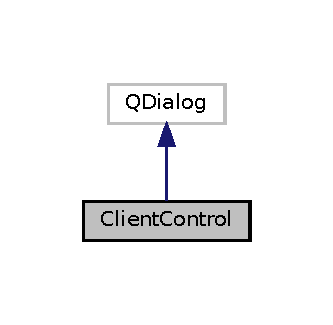
\includegraphics[width=160pt]{classClientControl__inherit__graph}
\end{center}
\end{figure}


Collaboration diagram for Client\+Control\+:
\nopagebreak
\begin{figure}[H]
\begin{center}
\leavevmode
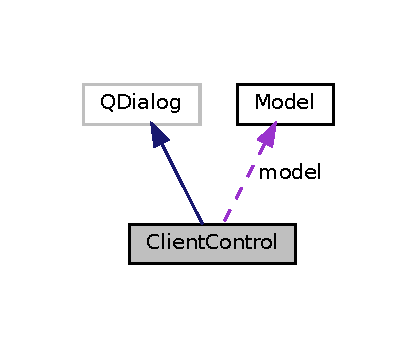
\includegraphics[width=200pt]{classClientControl__coll__graph}
\end{center}
\end{figure}
\subsection*{Public Member Functions}
\begin{DoxyCompactItemize}
\item 
\hyperlink{classClientControl_a2324d7192355735436aea9bfc7f84a5b}{Client\+Control} (Q\+Widget $\ast$parent=nullptr)
\begin{DoxyCompactList}\small\item\em Construct a new Client Control object. \end{DoxyCompactList}\item 
\hyperlink{classClientControl_aaa2a3d2e93433ddc9256d34911d9b9bd}{$\sim$\+Client\+Control} ()
\begin{DoxyCompactList}\small\item\em Destroy the Client Control object. \end{DoxyCompactList}\item 
\hyperlink{classModel}{Model} $\ast$ \hyperlink{classClientControl_aefc43486831b9e545a678abae5c592ca}{get\+Model} () const
\begin{DoxyCompactList}\small\item\em Get the \hyperlink{classModel}{Model} object. \end{DoxyCompactList}\item 
void \hyperlink{classClientControl_a3713d76eb6439b0764809e49bc7662ee}{set\+Model} (\hyperlink{classModel}{Model} $\ast$value)
\begin{DoxyCompactList}\small\item\em Set the \hyperlink{classModel}{Model} object. \end{DoxyCompactList}\item 
void \hyperlink{classClientControl_aa3d376fbe49768251c1bf674a10c9944}{set\+Table\+Data} ()
\begin{DoxyCompactList}\small\item\em Set the Table Data object. \end{DoxyCompactList}\item 
void \hyperlink{classClientControl_ab599f87b2be620b137cdfc4eaa060e58}{load\+\_\+course\+\_\+data} ()
\begin{DoxyCompactList}\small\item\em Load the courses to Table Widget. \end{DoxyCompactList}\item 
void \hyperlink{classClientControl_a826a7dc819e15623625da76b4c66f396}{load\+\_\+user\+\_\+data} ()
\begin{DoxyCompactList}\small\item\em Load the users to Table Widget. \end{DoxyCompactList}\end{DoxyCompactItemize}
\subsection*{Private Slots}
\begin{DoxyCompactItemize}
\item 
void \hyperlink{classClientControl_a8f9b32ace74f3152e1781ca73d60a90d}{on\+\_\+push\+Button\+\_\+clicked} ()
\begin{DoxyCompactList}\small\item\em function to edit course \end{DoxyCompactList}\item 
void \hyperlink{classClientControl_a8d716e92624ff6d05525dfee0fbd9a30}{on\+\_\+tab\+Widget\+\_\+current\+Changed} (int index)
\begin{DoxyCompactList}\small\item\em function to load table\textquotesingle{}s data \end{DoxyCompactList}\item 
void \hyperlink{classClientControl_a830f0e76e43c64fee40bbcd542e1e355}{edit\+\_\+course\+\_\+button\+\_\+pressed} ()
\begin{DoxyCompactList}\small\item\em function to edit course \end{DoxyCompactList}\item 
void \hyperlink{classClientControl_a759a2a2c0470f7903e053ef534cea4db}{remove\+\_\+course\+\_\+button\+\_\+pressed} ()
\begin{DoxyCompactList}\small\item\em function to remove course \end{DoxyCompactList}\item 
void \hyperlink{classClientControl_a09604fd71dee98f12cd46c3252f1cabe}{remove\+\_\+user\+\_\+pressed} ()
\begin{DoxyCompactList}\small\item\em function to remove user \end{DoxyCompactList}\item 
void \hyperlink{classClientControl_a2c9466ca951a1b8c32f24e4ab1389ba5}{edit\+\_\+user\+\_\+pressed} ()
\begin{DoxyCompactList}\small\item\em function to edit user \end{DoxyCompactList}\item 
void \hyperlink{classClientControl_a52bd587841a7a49f3e86ca09c2e3372d}{on\+\_\+exit\+\_\+adm\+\_\+btn\+\_\+clicked} ()
\begin{DoxyCompactList}\small\item\em function to logout \end{DoxyCompactList}\item 
void \hyperlink{classClientControl_a727cca41aa894d4cf371cfbba6f961d1}{on\+\_\+add\+\_\+user\+\_\+btn\+\_\+clicked} ()
\begin{DoxyCompactList}\small\item\em function to user insertion \end{DoxyCompactList}\item 
void \hyperlink{classClientControl_a5a380eab783cb0fc1760417956cec0d5}{on\+\_\+tab\+Widget\+\_\+tab\+Bar\+Clicked} (int index)
\begin{DoxyCompactList}\small\item\em load the Table Widget data \end{DoxyCompactList}\item 
void \hyperlink{classClientControl_a8a46c9d7c91c26e0f4b779452cea8208}{on\+\_\+cancel\+\_\+client\+\_\+btn\+\_\+clicked} ()
\begin{DoxyCompactList}\small\item\em Cancel user insertion. \end{DoxyCompactList}\item 
void \hyperlink{classClientControl_a4771dbff3cfafb5d34d55a009cb073ff}{on\+\_\+cancel\+\_\+course\+\_\+btn\+\_\+clicked} ()
\begin{DoxyCompactList}\small\item\em Cancel course insertion. \end{DoxyCompactList}\end{DoxyCompactItemize}
\subsection*{Private Attributes}
\begin{DoxyCompactItemize}
\item 
Ui\+::\+Client\+Control $\ast$ \hyperlink{classClientControl_adea5f2cf529bedcc7d2aac9e2702d702}{ui}
\item 
\hyperlink{classModel}{Model} $\ast$ \hyperlink{classClientControl_a58fe6ae8049d307caa62f164a8c07eed}{model}
\end{DoxyCompactItemize}


\subsection{Detailed Description}
this class represents the Adm Page 

\subsection{Constructor \& Destructor Documentation}
\mbox{\Hypertarget{classClientControl_a2324d7192355735436aea9bfc7f84a5b}\label{classClientControl_a2324d7192355735436aea9bfc7f84a5b}} 
\index{Client\+Control@{Client\+Control}!Client\+Control@{Client\+Control}}
\index{Client\+Control@{Client\+Control}!Client\+Control@{Client\+Control}}
\subsubsection{\texorpdfstring{Client\+Control()}{ClientControl()}}
{\footnotesize\ttfamily Client\+Control\+::\+Client\+Control (\begin{DoxyParamCaption}\item[{Q\+Widget $\ast$}]{parent = {\ttfamily nullptr} }\end{DoxyParamCaption})\hspace{0.3cm}{\ttfamily [explicit]}}



Construct a new Client Control object. 


\begin{DoxyParams}{Parameters}
{\em parent} & \\
\hline
\end{DoxyParams}
\mbox{\Hypertarget{classClientControl_aaa2a3d2e93433ddc9256d34911d9b9bd}\label{classClientControl_aaa2a3d2e93433ddc9256d34911d9b9bd}} 
\index{Client\+Control@{Client\+Control}!````~Client\+Control@{$\sim$\+Client\+Control}}
\index{````~Client\+Control@{$\sim$\+Client\+Control}!Client\+Control@{Client\+Control}}
\subsubsection{\texorpdfstring{$\sim$\+Client\+Control()}{~ClientControl()}}
{\footnotesize\ttfamily Client\+Control\+::$\sim$\+Client\+Control (\begin{DoxyParamCaption}{ }\end{DoxyParamCaption})}



Destroy the Client Control object. 



\subsection{Member Function Documentation}
\mbox{\Hypertarget{classClientControl_a830f0e76e43c64fee40bbcd542e1e355}\label{classClientControl_a830f0e76e43c64fee40bbcd542e1e355}} 
\index{Client\+Control@{Client\+Control}!edit\+\_\+course\+\_\+button\+\_\+pressed@{edit\+\_\+course\+\_\+button\+\_\+pressed}}
\index{edit\+\_\+course\+\_\+button\+\_\+pressed@{edit\+\_\+course\+\_\+button\+\_\+pressed}!Client\+Control@{Client\+Control}}
\subsubsection{\texorpdfstring{edit\+\_\+course\+\_\+button\+\_\+pressed}{edit\_course\_button\_pressed}}
{\footnotesize\ttfamily void Client\+Control\+::edit\+\_\+course\+\_\+button\+\_\+pressed (\begin{DoxyParamCaption}{ }\end{DoxyParamCaption})\hspace{0.3cm}{\ttfamily [private]}, {\ttfamily [slot]}}



function to edit course 

\mbox{\Hypertarget{classClientControl_a2c9466ca951a1b8c32f24e4ab1389ba5}\label{classClientControl_a2c9466ca951a1b8c32f24e4ab1389ba5}} 
\index{Client\+Control@{Client\+Control}!edit\+\_\+user\+\_\+pressed@{edit\+\_\+user\+\_\+pressed}}
\index{edit\+\_\+user\+\_\+pressed@{edit\+\_\+user\+\_\+pressed}!Client\+Control@{Client\+Control}}
\subsubsection{\texorpdfstring{edit\+\_\+user\+\_\+pressed}{edit\_user\_pressed}}
{\footnotesize\ttfamily void Client\+Control\+::edit\+\_\+user\+\_\+pressed (\begin{DoxyParamCaption}{ }\end{DoxyParamCaption})\hspace{0.3cm}{\ttfamily [private]}, {\ttfamily [slot]}}



function to edit user 

\mbox{\Hypertarget{classClientControl_aefc43486831b9e545a678abae5c592ca}\label{classClientControl_aefc43486831b9e545a678abae5c592ca}} 
\index{Client\+Control@{Client\+Control}!get\+Model@{get\+Model}}
\index{get\+Model@{get\+Model}!Client\+Control@{Client\+Control}}
\subsubsection{\texorpdfstring{get\+Model()}{getModel()}}
{\footnotesize\ttfamily \hyperlink{classModel}{Model} $\ast$ Client\+Control\+::get\+Model (\begin{DoxyParamCaption}{ }\end{DoxyParamCaption}) const}



Get the \hyperlink{classModel}{Model} object. 

\begin{DoxyReturn}{Returns}
Model$\ast$ the page\textquotesingle{}s model 
\end{DoxyReturn}
\mbox{\Hypertarget{classClientControl_ab599f87b2be620b137cdfc4eaa060e58}\label{classClientControl_ab599f87b2be620b137cdfc4eaa060e58}} 
\index{Client\+Control@{Client\+Control}!load\+\_\+course\+\_\+data@{load\+\_\+course\+\_\+data}}
\index{load\+\_\+course\+\_\+data@{load\+\_\+course\+\_\+data}!Client\+Control@{Client\+Control}}
\subsubsection{\texorpdfstring{load\+\_\+course\+\_\+data()}{load\_course\_data()}}
{\footnotesize\ttfamily void Client\+Control\+::load\+\_\+course\+\_\+data (\begin{DoxyParamCaption}{ }\end{DoxyParamCaption})}



Load the courses to Table Widget. 

\mbox{\Hypertarget{classClientControl_a826a7dc819e15623625da76b4c66f396}\label{classClientControl_a826a7dc819e15623625da76b4c66f396}} 
\index{Client\+Control@{Client\+Control}!load\+\_\+user\+\_\+data@{load\+\_\+user\+\_\+data}}
\index{load\+\_\+user\+\_\+data@{load\+\_\+user\+\_\+data}!Client\+Control@{Client\+Control}}
\subsubsection{\texorpdfstring{load\+\_\+user\+\_\+data()}{load\_user\_data()}}
{\footnotesize\ttfamily void Client\+Control\+::load\+\_\+user\+\_\+data (\begin{DoxyParamCaption}{ }\end{DoxyParamCaption})}



Load the users to Table Widget. 

\mbox{\Hypertarget{classClientControl_a727cca41aa894d4cf371cfbba6f961d1}\label{classClientControl_a727cca41aa894d4cf371cfbba6f961d1}} 
\index{Client\+Control@{Client\+Control}!on\+\_\+add\+\_\+user\+\_\+btn\+\_\+clicked@{on\+\_\+add\+\_\+user\+\_\+btn\+\_\+clicked}}
\index{on\+\_\+add\+\_\+user\+\_\+btn\+\_\+clicked@{on\+\_\+add\+\_\+user\+\_\+btn\+\_\+clicked}!Client\+Control@{Client\+Control}}
\subsubsection{\texorpdfstring{on\+\_\+add\+\_\+user\+\_\+btn\+\_\+clicked}{on\_add\_user\_btn\_clicked}}
{\footnotesize\ttfamily void Client\+Control\+::on\+\_\+add\+\_\+user\+\_\+btn\+\_\+clicked (\begin{DoxyParamCaption}{ }\end{DoxyParamCaption})\hspace{0.3cm}{\ttfamily [private]}, {\ttfamily [slot]}}



function to user insertion 

\mbox{\Hypertarget{classClientControl_a8a46c9d7c91c26e0f4b779452cea8208}\label{classClientControl_a8a46c9d7c91c26e0f4b779452cea8208}} 
\index{Client\+Control@{Client\+Control}!on\+\_\+cancel\+\_\+client\+\_\+btn\+\_\+clicked@{on\+\_\+cancel\+\_\+client\+\_\+btn\+\_\+clicked}}
\index{on\+\_\+cancel\+\_\+client\+\_\+btn\+\_\+clicked@{on\+\_\+cancel\+\_\+client\+\_\+btn\+\_\+clicked}!Client\+Control@{Client\+Control}}
\subsubsection{\texorpdfstring{on\+\_\+cancel\+\_\+client\+\_\+btn\+\_\+clicked}{on\_cancel\_client\_btn\_clicked}}
{\footnotesize\ttfamily void Client\+Control\+::on\+\_\+cancel\+\_\+client\+\_\+btn\+\_\+clicked (\begin{DoxyParamCaption}{ }\end{DoxyParamCaption})\hspace{0.3cm}{\ttfamily [private]}, {\ttfamily [slot]}}



Cancel user insertion. 

\mbox{\Hypertarget{classClientControl_a4771dbff3cfafb5d34d55a009cb073ff}\label{classClientControl_a4771dbff3cfafb5d34d55a009cb073ff}} 
\index{Client\+Control@{Client\+Control}!on\+\_\+cancel\+\_\+course\+\_\+btn\+\_\+clicked@{on\+\_\+cancel\+\_\+course\+\_\+btn\+\_\+clicked}}
\index{on\+\_\+cancel\+\_\+course\+\_\+btn\+\_\+clicked@{on\+\_\+cancel\+\_\+course\+\_\+btn\+\_\+clicked}!Client\+Control@{Client\+Control}}
\subsubsection{\texorpdfstring{on\+\_\+cancel\+\_\+course\+\_\+btn\+\_\+clicked}{on\_cancel\_course\_btn\_clicked}}
{\footnotesize\ttfamily void Client\+Control\+::on\+\_\+cancel\+\_\+course\+\_\+btn\+\_\+clicked (\begin{DoxyParamCaption}{ }\end{DoxyParamCaption})\hspace{0.3cm}{\ttfamily [private]}, {\ttfamily [slot]}}



Cancel course insertion. 

\mbox{\Hypertarget{classClientControl_a52bd587841a7a49f3e86ca09c2e3372d}\label{classClientControl_a52bd587841a7a49f3e86ca09c2e3372d}} 
\index{Client\+Control@{Client\+Control}!on\+\_\+exit\+\_\+adm\+\_\+btn\+\_\+clicked@{on\+\_\+exit\+\_\+adm\+\_\+btn\+\_\+clicked}}
\index{on\+\_\+exit\+\_\+adm\+\_\+btn\+\_\+clicked@{on\+\_\+exit\+\_\+adm\+\_\+btn\+\_\+clicked}!Client\+Control@{Client\+Control}}
\subsubsection{\texorpdfstring{on\+\_\+exit\+\_\+adm\+\_\+btn\+\_\+clicked}{on\_exit\_adm\_btn\_clicked}}
{\footnotesize\ttfamily void Client\+Control\+::on\+\_\+exit\+\_\+adm\+\_\+btn\+\_\+clicked (\begin{DoxyParamCaption}{ }\end{DoxyParamCaption})\hspace{0.3cm}{\ttfamily [private]}, {\ttfamily [slot]}}



function to logout 

\mbox{\Hypertarget{classClientControl_a8f9b32ace74f3152e1781ca73d60a90d}\label{classClientControl_a8f9b32ace74f3152e1781ca73d60a90d}} 
\index{Client\+Control@{Client\+Control}!on\+\_\+push\+Button\+\_\+clicked@{on\+\_\+push\+Button\+\_\+clicked}}
\index{on\+\_\+push\+Button\+\_\+clicked@{on\+\_\+push\+Button\+\_\+clicked}!Client\+Control@{Client\+Control}}
\subsubsection{\texorpdfstring{on\+\_\+push\+Button\+\_\+clicked}{on\_pushButton\_clicked}}
{\footnotesize\ttfamily void Client\+Control\+::on\+\_\+push\+Button\+\_\+clicked (\begin{DoxyParamCaption}{ }\end{DoxyParamCaption})\hspace{0.3cm}{\ttfamily [private]}, {\ttfamily [slot]}}



function to edit course 

\mbox{\Hypertarget{classClientControl_a8d716e92624ff6d05525dfee0fbd9a30}\label{classClientControl_a8d716e92624ff6d05525dfee0fbd9a30}} 
\index{Client\+Control@{Client\+Control}!on\+\_\+tab\+Widget\+\_\+current\+Changed@{on\+\_\+tab\+Widget\+\_\+current\+Changed}}
\index{on\+\_\+tab\+Widget\+\_\+current\+Changed@{on\+\_\+tab\+Widget\+\_\+current\+Changed}!Client\+Control@{Client\+Control}}
\subsubsection{\texorpdfstring{on\+\_\+tab\+Widget\+\_\+current\+Changed}{on\_tabWidget\_currentChanged}}
{\footnotesize\ttfamily void Client\+Control\+::on\+\_\+tab\+Widget\+\_\+current\+Changed (\begin{DoxyParamCaption}\item[{int}]{index }\end{DoxyParamCaption})\hspace{0.3cm}{\ttfamily [private]}, {\ttfamily [slot]}}



function to load table\textquotesingle{}s data 


\begin{DoxyParams}{Parameters}
{\em index} & the aba index \\
\hline
\end{DoxyParams}
\mbox{\Hypertarget{classClientControl_a5a380eab783cb0fc1760417956cec0d5}\label{classClientControl_a5a380eab783cb0fc1760417956cec0d5}} 
\index{Client\+Control@{Client\+Control}!on\+\_\+tab\+Widget\+\_\+tab\+Bar\+Clicked@{on\+\_\+tab\+Widget\+\_\+tab\+Bar\+Clicked}}
\index{on\+\_\+tab\+Widget\+\_\+tab\+Bar\+Clicked@{on\+\_\+tab\+Widget\+\_\+tab\+Bar\+Clicked}!Client\+Control@{Client\+Control}}
\subsubsection{\texorpdfstring{on\+\_\+tab\+Widget\+\_\+tab\+Bar\+Clicked}{on\_tabWidget\_tabBarClicked}}
{\footnotesize\ttfamily void Client\+Control\+::on\+\_\+tab\+Widget\+\_\+tab\+Bar\+Clicked (\begin{DoxyParamCaption}\item[{int}]{index }\end{DoxyParamCaption})\hspace{0.3cm}{\ttfamily [private]}, {\ttfamily [slot]}}



load the Table Widget data 


\begin{DoxyParams}{Parameters}
{\em index} & \\
\hline
\end{DoxyParams}
\mbox{\Hypertarget{classClientControl_a759a2a2c0470f7903e053ef534cea4db}\label{classClientControl_a759a2a2c0470f7903e053ef534cea4db}} 
\index{Client\+Control@{Client\+Control}!remove\+\_\+course\+\_\+button\+\_\+pressed@{remove\+\_\+course\+\_\+button\+\_\+pressed}}
\index{remove\+\_\+course\+\_\+button\+\_\+pressed@{remove\+\_\+course\+\_\+button\+\_\+pressed}!Client\+Control@{Client\+Control}}
\subsubsection{\texorpdfstring{remove\+\_\+course\+\_\+button\+\_\+pressed}{remove\_course\_button\_pressed}}
{\footnotesize\ttfamily void Client\+Control\+::remove\+\_\+course\+\_\+button\+\_\+pressed (\begin{DoxyParamCaption}{ }\end{DoxyParamCaption})\hspace{0.3cm}{\ttfamily [private]}, {\ttfamily [slot]}}



function to remove course 

\mbox{\Hypertarget{classClientControl_a09604fd71dee98f12cd46c3252f1cabe}\label{classClientControl_a09604fd71dee98f12cd46c3252f1cabe}} 
\index{Client\+Control@{Client\+Control}!remove\+\_\+user\+\_\+pressed@{remove\+\_\+user\+\_\+pressed}}
\index{remove\+\_\+user\+\_\+pressed@{remove\+\_\+user\+\_\+pressed}!Client\+Control@{Client\+Control}}
\subsubsection{\texorpdfstring{remove\+\_\+user\+\_\+pressed}{remove\_user\_pressed}}
{\footnotesize\ttfamily void Client\+Control\+::remove\+\_\+user\+\_\+pressed (\begin{DoxyParamCaption}{ }\end{DoxyParamCaption})\hspace{0.3cm}{\ttfamily [private]}, {\ttfamily [slot]}}



function to remove user 

\mbox{\Hypertarget{classClientControl_a3713d76eb6439b0764809e49bc7662ee}\label{classClientControl_a3713d76eb6439b0764809e49bc7662ee}} 
\index{Client\+Control@{Client\+Control}!set\+Model@{set\+Model}}
\index{set\+Model@{set\+Model}!Client\+Control@{Client\+Control}}
\subsubsection{\texorpdfstring{set\+Model()}{setModel()}}
{\footnotesize\ttfamily void Client\+Control\+::set\+Model (\begin{DoxyParamCaption}\item[{\hyperlink{classModel}{Model} $\ast$}]{value }\end{DoxyParamCaption})}



Set the \hyperlink{classModel}{Model} object. 


\begin{DoxyParams}{Parameters}
{\em value} & the new page\textquotesingle{}s model \\
\hline
\end{DoxyParams}
\mbox{\Hypertarget{classClientControl_aa3d376fbe49768251c1bf674a10c9944}\label{classClientControl_aa3d376fbe49768251c1bf674a10c9944}} 
\index{Client\+Control@{Client\+Control}!set\+Table\+Data@{set\+Table\+Data}}
\index{set\+Table\+Data@{set\+Table\+Data}!Client\+Control@{Client\+Control}}
\subsubsection{\texorpdfstring{set\+Table\+Data()}{setTableData()}}
{\footnotesize\ttfamily void Client\+Control\+::set\+Table\+Data (\begin{DoxyParamCaption}{ }\end{DoxyParamCaption})}



Set the Table Data object. 



\subsection{Member Data Documentation}
\mbox{\Hypertarget{classClientControl_a58fe6ae8049d307caa62f164a8c07eed}\label{classClientControl_a58fe6ae8049d307caa62f164a8c07eed}} 
\index{Client\+Control@{Client\+Control}!model@{model}}
\index{model@{model}!Client\+Control@{Client\+Control}}
\subsubsection{\texorpdfstring{model}{model}}
{\footnotesize\ttfamily \hyperlink{classModel}{Model}$\ast$ Client\+Control\+::model\hspace{0.3cm}{\ttfamily [private]}}

\mbox{\Hypertarget{classClientControl_adea5f2cf529bedcc7d2aac9e2702d702}\label{classClientControl_adea5f2cf529bedcc7d2aac9e2702d702}} 
\index{Client\+Control@{Client\+Control}!ui@{ui}}
\index{ui@{ui}!Client\+Control@{Client\+Control}}
\subsubsection{\texorpdfstring{ui}{ui}}
{\footnotesize\ttfamily Ui\+::\+Client\+Control$\ast$ Client\+Control\+::ui\hspace{0.3cm}{\ttfamily [private]}}



The documentation for this class was generated from the following files\+:\begin{DoxyCompactItemize}
\item 
views/\hyperlink{clientcontrol_8h}{clientcontrol.\+h}\item 
views/\hyperlink{clientcontrol_8cpp}{clientcontrol.\+cpp}\end{DoxyCompactItemize}

\hypertarget{classclientPage}{}\section{client\+Page Class Reference}
\label{classclientPage}\index{client\+Page@{client\+Page}}


{\ttfamily \#include $<$clientpage.\+h$>$}



Inheritance diagram for client\+Page\+:\nopagebreak
\begin{figure}[H]
\begin{center}
\leavevmode
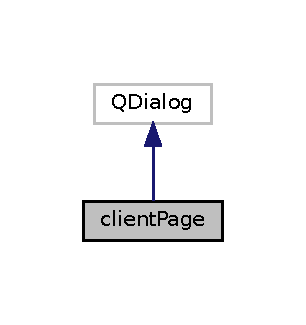
\includegraphics[width=147pt]{classclientPage__inherit__graph}
\end{center}
\end{figure}


Collaboration diagram for client\+Page\+:\nopagebreak
\begin{figure}[H]
\begin{center}
\leavevmode
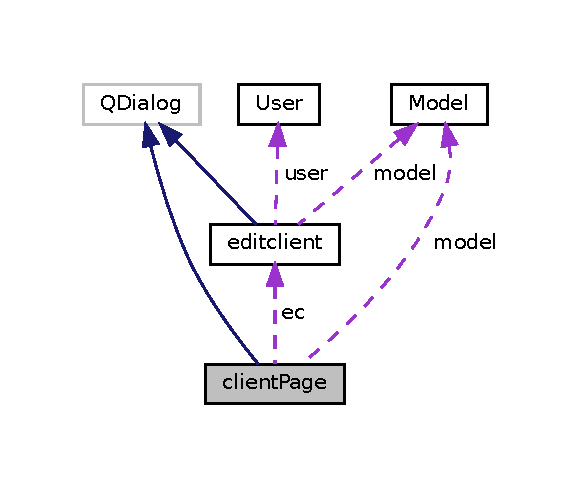
\includegraphics[width=279pt]{classclientPage__coll__graph}
\end{center}
\end{figure}
\subsection*{Public Member Functions}
\begin{DoxyCompactItemize}
\item 
\hyperlink{classclientPage_ad0e43d381003fa34cf0151fc96896da3}{client\+Page} (Q\+Widget $\ast$parent=nullptr)
\begin{DoxyCompactList}\small\item\em Construct a new client Page object. \end{DoxyCompactList}\item 
\hyperlink{classclientPage_af0c9562c16a80c54686adbc6f9637ebc}{$\sim$client\+Page} ()
\begin{DoxyCompactList}\small\item\em Destroy the client Page object. \end{DoxyCompactList}\item 
\hyperlink{classModel}{Model} $\ast$ \hyperlink{classclientPage_ab2876735aef44d0e72f7a57820148a27}{get\+Model} () const
\begin{DoxyCompactList}\small\item\em Get the \hyperlink{classModel}{Model} object. \end{DoxyCompactList}\item 
void \hyperlink{classclientPage_ac40930f54077f9a7050e046b535ed45c}{set\+Model} (\hyperlink{classModel}{Model} $\ast$value)
\begin{DoxyCompactList}\small\item\em Set the \hyperlink{classModel}{Model} object. \end{DoxyCompactList}\item 
\hyperlink{classeditclient}{editclient} $\ast$ \hyperlink{classclientPage_aa61872884ea03691d0ac38db4d0d01cc}{get\+Edit\+Client} () const
\begin{DoxyCompactList}\small\item\em Get the Login object. \end{DoxyCompactList}\item 
void \hyperlink{classclientPage_ab16c72bc9c44d5e833206133d692c857}{set\+Edit\+Client} (\hyperlink{classeditclient}{editclient} $\ast$value)
\begin{DoxyCompactList}\small\item\em Set the Login object. \end{DoxyCompactList}\item 
void \hyperlink{classclientPage_aa430c4866eaf46e93492d4b950443689}{set\+Table\+Data} ()
\begin{DoxyCompactList}\small\item\em Configure the Table\+Widget objects. \end{DoxyCompactList}\item 
void \hyperlink{classclientPage_af7655cb029199e82bb1116969bc695e2}{load\+\_\+client\+\_\+courses} (const vector$<$ \hyperlink{classCourse}{Course} $\ast$$>$ \&)
\begin{DoxyCompactList}\small\item\em Load the Client\textquotesingle{}s courses. \end{DoxyCompactList}\item 
void \hyperlink{classclientPage_ae5b2455576f3b750131cd21b5bb08430}{load\+\_\+all\+\_\+courses} (const vector$<$ \hyperlink{classCourse}{Course} $\ast$$>$ \&)
\begin{DoxyCompactList}\small\item\em Load all the \hyperlink{classModel}{Model}\textquotesingle{}s courses. \end{DoxyCompactList}\end{DoxyCompactItemize}
\subsection*{Private Slots}
\begin{DoxyCompactItemize}
\item 
void \hyperlink{classclientPage_a4e6a1fa2748827eeebac3ec6ec8ca2b9}{buy\+\_\+button\+\_\+pressed} ()
\begin{DoxyCompactList}\small\item\em function to buy a new course \end{DoxyCompactList}\item 
void \hyperlink{classclientPage_a71689a732ff9823c892105996593084b}{on\+\_\+edit\+\_\+profile\+\_\+btn\+\_\+clicked} ()
\begin{DoxyCompactList}\small\item\em function to edit a user \end{DoxyCompactList}\item 
void \hyperlink{classclientPage_a8485bac1ad742c7fe4bb4b14a504b506}{on\+\_\+tab\+Widget\+\_\+current\+Changed} (int index)
\begin{DoxyCompactList}\small\item\em function to reload the table data when necesary \end{DoxyCompactList}\item 
void \hyperlink{classclientPage_aaa4bc6d404c46a5d066fd566e902f5d9}{on\+\_\+logout\+\_\+btn\+\_\+clicked} ()
\begin{DoxyCompactList}\small\item\em function to logout \end{DoxyCompactList}\item 
void \hyperlink{classclientPage_a48bd84cbd67d5fad6a221b400c3e95e7}{on\+\_\+tab\+Widget\+\_\+tab\+Bar\+Clicked} (int index)
\begin{DoxyCompactList}\small\item\em function do load the table data \end{DoxyCompactList}\item 
void \hyperlink{classclientPage_ab2b6ddcf0b2a65919802226ac692cab9}{on\+\_\+btn\+\_\+search\+\_\+new\+\_\+clicked} ()
\begin{DoxyCompactList}\small\item\em function to search courses \end{DoxyCompactList}\item 
void \hyperlink{classclientPage_aba1c12dd43662d34b989a250af96c0aa}{on\+\_\+btn\+\_\+search\+\_\+clicked} ()
\begin{DoxyCompactList}\small\item\em function to throw the search \end{DoxyCompactList}\end{DoxyCompactItemize}
\subsection*{Private Attributes}
\begin{DoxyCompactItemize}
\item 
Ui\+::client\+Page $\ast$ \hyperlink{classclientPage_a1c0ad34f6a6dc4eb84713d0c770ee27a}{ui}
\item 
\hyperlink{classModel}{Model} $\ast$ \hyperlink{classclientPage_a21b8604c7b8285a3ba9c37b133f89f02}{model}
\item 
\hyperlink{classeditclient}{editclient} $\ast$ \hyperlink{classclientPage_a70e3ec19ba9c4cbf70d9410173e97afd}{ec}
\end{DoxyCompactItemize}


\subsection{Constructor \& Destructor Documentation}
\mbox{\Hypertarget{classclientPage_ad0e43d381003fa34cf0151fc96896da3}\label{classclientPage_ad0e43d381003fa34cf0151fc96896da3}} 
\index{client\+Page@{client\+Page}!client\+Page@{client\+Page}}
\index{client\+Page@{client\+Page}!client\+Page@{client\+Page}}
\subsubsection{\texorpdfstring{client\+Page()}{clientPage()}}
{\footnotesize\ttfamily client\+Page\+::client\+Page (\begin{DoxyParamCaption}\item[{Q\+Widget $\ast$}]{parent = {\ttfamily nullptr} }\end{DoxyParamCaption})\hspace{0.3cm}{\ttfamily [explicit]}}



Construct a new client Page object. 


\begin{DoxyParams}{Parameters}
{\em parent} & \\
\hline
\end{DoxyParams}
\mbox{\Hypertarget{classclientPage_af0c9562c16a80c54686adbc6f9637ebc}\label{classclientPage_af0c9562c16a80c54686adbc6f9637ebc}} 
\index{client\+Page@{client\+Page}!````~client\+Page@{$\sim$client\+Page}}
\index{````~client\+Page@{$\sim$client\+Page}!client\+Page@{client\+Page}}
\subsubsection{\texorpdfstring{$\sim$client\+Page()}{~clientPage()}}
{\footnotesize\ttfamily client\+Page\+::$\sim$client\+Page (\begin{DoxyParamCaption}{ }\end{DoxyParamCaption})}



Destroy the client Page object. 



\subsection{Member Function Documentation}
\mbox{\Hypertarget{classclientPage_a4e6a1fa2748827eeebac3ec6ec8ca2b9}\label{classclientPage_a4e6a1fa2748827eeebac3ec6ec8ca2b9}} 
\index{client\+Page@{client\+Page}!buy\+\_\+button\+\_\+pressed@{buy\+\_\+button\+\_\+pressed}}
\index{buy\+\_\+button\+\_\+pressed@{buy\+\_\+button\+\_\+pressed}!client\+Page@{client\+Page}}
\subsubsection{\texorpdfstring{buy\+\_\+button\+\_\+pressed}{buy\_button\_pressed}}
{\footnotesize\ttfamily void client\+Page\+::buy\+\_\+button\+\_\+pressed (\begin{DoxyParamCaption}{ }\end{DoxyParamCaption})\hspace{0.3cm}{\ttfamily [private]}, {\ttfamily [slot]}}



function to buy a new course 

\mbox{\Hypertarget{classclientPage_aa61872884ea03691d0ac38db4d0d01cc}\label{classclientPage_aa61872884ea03691d0ac38db4d0d01cc}} 
\index{client\+Page@{client\+Page}!get\+Edit\+Client@{get\+Edit\+Client}}
\index{get\+Edit\+Client@{get\+Edit\+Client}!client\+Page@{client\+Page}}
\subsubsection{\texorpdfstring{get\+Edit\+Client()}{getEditClient()}}
{\footnotesize\ttfamily \hyperlink{classeditclient}{editclient} $\ast$ client\+Page\+::get\+Edit\+Client (\begin{DoxyParamCaption}{ }\end{DoxyParamCaption}) const}



Get the Login object. 

\begin{DoxyReturn}{Returns}
Login$\ast$ the login pointer 
\end{DoxyReturn}
\mbox{\Hypertarget{classclientPage_ab2876735aef44d0e72f7a57820148a27}\label{classclientPage_ab2876735aef44d0e72f7a57820148a27}} 
\index{client\+Page@{client\+Page}!get\+Model@{get\+Model}}
\index{get\+Model@{get\+Model}!client\+Page@{client\+Page}}
\subsubsection{\texorpdfstring{get\+Model()}{getModel()}}
{\footnotesize\ttfamily \hyperlink{classModel}{Model} $\ast$ client\+Page\+::get\+Model (\begin{DoxyParamCaption}{ }\end{DoxyParamCaption}) const}



Get the \hyperlink{classModel}{Model} object. 

\begin{DoxyReturn}{Returns}
Model$\ast$ the model pointer 
\end{DoxyReturn}
\mbox{\Hypertarget{classclientPage_ae5b2455576f3b750131cd21b5bb08430}\label{classclientPage_ae5b2455576f3b750131cd21b5bb08430}} 
\index{client\+Page@{client\+Page}!load\+\_\+all\+\_\+courses@{load\+\_\+all\+\_\+courses}}
\index{load\+\_\+all\+\_\+courses@{load\+\_\+all\+\_\+courses}!client\+Page@{client\+Page}}
\subsubsection{\texorpdfstring{load\+\_\+all\+\_\+courses()}{load\_all\_courses()}}
{\footnotesize\ttfamily void client\+Page\+::load\+\_\+all\+\_\+courses (\begin{DoxyParamCaption}\item[{const vector$<$ \hyperlink{classCourse}{Course} $\ast$$>$ \&}]{courses }\end{DoxyParamCaption})}



Load all the \hyperlink{classModel}{Model}\textquotesingle{}s courses. 

\mbox{\Hypertarget{classclientPage_af7655cb029199e82bb1116969bc695e2}\label{classclientPage_af7655cb029199e82bb1116969bc695e2}} 
\index{client\+Page@{client\+Page}!load\+\_\+client\+\_\+courses@{load\+\_\+client\+\_\+courses}}
\index{load\+\_\+client\+\_\+courses@{load\+\_\+client\+\_\+courses}!client\+Page@{client\+Page}}
\subsubsection{\texorpdfstring{load\+\_\+client\+\_\+courses()}{load\_client\_courses()}}
{\footnotesize\ttfamily void client\+Page\+::load\+\_\+client\+\_\+courses (\begin{DoxyParamCaption}\item[{const vector$<$ \hyperlink{classCourse}{Course} $\ast$$>$ \&}]{courses }\end{DoxyParamCaption})}



Load the Client\textquotesingle{}s courses. 

\mbox{\Hypertarget{classclientPage_aba1c12dd43662d34b989a250af96c0aa}\label{classclientPage_aba1c12dd43662d34b989a250af96c0aa}} 
\index{client\+Page@{client\+Page}!on\+\_\+btn\+\_\+search\+\_\+clicked@{on\+\_\+btn\+\_\+search\+\_\+clicked}}
\index{on\+\_\+btn\+\_\+search\+\_\+clicked@{on\+\_\+btn\+\_\+search\+\_\+clicked}!client\+Page@{client\+Page}}
\subsubsection{\texorpdfstring{on\+\_\+btn\+\_\+search\+\_\+clicked}{on\_btn\_search\_clicked}}
{\footnotesize\ttfamily void client\+Page\+::on\+\_\+btn\+\_\+search\+\_\+clicked (\begin{DoxyParamCaption}{ }\end{DoxyParamCaption})\hspace{0.3cm}{\ttfamily [private]}, {\ttfamily [slot]}}



function to throw the search 

\mbox{\Hypertarget{classclientPage_ab2b6ddcf0b2a65919802226ac692cab9}\label{classclientPage_ab2b6ddcf0b2a65919802226ac692cab9}} 
\index{client\+Page@{client\+Page}!on\+\_\+btn\+\_\+search\+\_\+new\+\_\+clicked@{on\+\_\+btn\+\_\+search\+\_\+new\+\_\+clicked}}
\index{on\+\_\+btn\+\_\+search\+\_\+new\+\_\+clicked@{on\+\_\+btn\+\_\+search\+\_\+new\+\_\+clicked}!client\+Page@{client\+Page}}
\subsubsection{\texorpdfstring{on\+\_\+btn\+\_\+search\+\_\+new\+\_\+clicked}{on\_btn\_search\_new\_clicked}}
{\footnotesize\ttfamily void client\+Page\+::on\+\_\+btn\+\_\+search\+\_\+new\+\_\+clicked (\begin{DoxyParamCaption}{ }\end{DoxyParamCaption})\hspace{0.3cm}{\ttfamily [private]}, {\ttfamily [slot]}}



function to search courses 

\mbox{\Hypertarget{classclientPage_a71689a732ff9823c892105996593084b}\label{classclientPage_a71689a732ff9823c892105996593084b}} 
\index{client\+Page@{client\+Page}!on\+\_\+edit\+\_\+profile\+\_\+btn\+\_\+clicked@{on\+\_\+edit\+\_\+profile\+\_\+btn\+\_\+clicked}}
\index{on\+\_\+edit\+\_\+profile\+\_\+btn\+\_\+clicked@{on\+\_\+edit\+\_\+profile\+\_\+btn\+\_\+clicked}!client\+Page@{client\+Page}}
\subsubsection{\texorpdfstring{on\+\_\+edit\+\_\+profile\+\_\+btn\+\_\+clicked}{on\_edit\_profile\_btn\_clicked}}
{\footnotesize\ttfamily void client\+Page\+::on\+\_\+edit\+\_\+profile\+\_\+btn\+\_\+clicked (\begin{DoxyParamCaption}{ }\end{DoxyParamCaption})\hspace{0.3cm}{\ttfamily [private]}, {\ttfamily [slot]}}



function to edit a user 

\mbox{\Hypertarget{classclientPage_aaa4bc6d404c46a5d066fd566e902f5d9}\label{classclientPage_aaa4bc6d404c46a5d066fd566e902f5d9}} 
\index{client\+Page@{client\+Page}!on\+\_\+logout\+\_\+btn\+\_\+clicked@{on\+\_\+logout\+\_\+btn\+\_\+clicked}}
\index{on\+\_\+logout\+\_\+btn\+\_\+clicked@{on\+\_\+logout\+\_\+btn\+\_\+clicked}!client\+Page@{client\+Page}}
\subsubsection{\texorpdfstring{on\+\_\+logout\+\_\+btn\+\_\+clicked}{on\_logout\_btn\_clicked}}
{\footnotesize\ttfamily void client\+Page\+::on\+\_\+logout\+\_\+btn\+\_\+clicked (\begin{DoxyParamCaption}{ }\end{DoxyParamCaption})\hspace{0.3cm}{\ttfamily [private]}, {\ttfamily [slot]}}



function to logout 

\mbox{\Hypertarget{classclientPage_a8485bac1ad742c7fe4bb4b14a504b506}\label{classclientPage_a8485bac1ad742c7fe4bb4b14a504b506}} 
\index{client\+Page@{client\+Page}!on\+\_\+tab\+Widget\+\_\+current\+Changed@{on\+\_\+tab\+Widget\+\_\+current\+Changed}}
\index{on\+\_\+tab\+Widget\+\_\+current\+Changed@{on\+\_\+tab\+Widget\+\_\+current\+Changed}!client\+Page@{client\+Page}}
\subsubsection{\texorpdfstring{on\+\_\+tab\+Widget\+\_\+current\+Changed}{on\_tabWidget\_currentChanged}}
{\footnotesize\ttfamily void client\+Page\+::on\+\_\+tab\+Widget\+\_\+current\+Changed (\begin{DoxyParamCaption}\item[{int}]{index }\end{DoxyParamCaption})\hspace{0.3cm}{\ttfamily [private]}, {\ttfamily [slot]}}



function to reload the table data when necesary 


\begin{DoxyParams}{Parameters}
{\em index} & \\
\hline
\end{DoxyParams}
\mbox{\Hypertarget{classclientPage_a48bd84cbd67d5fad6a221b400c3e95e7}\label{classclientPage_a48bd84cbd67d5fad6a221b400c3e95e7}} 
\index{client\+Page@{client\+Page}!on\+\_\+tab\+Widget\+\_\+tab\+Bar\+Clicked@{on\+\_\+tab\+Widget\+\_\+tab\+Bar\+Clicked}}
\index{on\+\_\+tab\+Widget\+\_\+tab\+Bar\+Clicked@{on\+\_\+tab\+Widget\+\_\+tab\+Bar\+Clicked}!client\+Page@{client\+Page}}
\subsubsection{\texorpdfstring{on\+\_\+tab\+Widget\+\_\+tab\+Bar\+Clicked}{on\_tabWidget\_tabBarClicked}}
{\footnotesize\ttfamily void client\+Page\+::on\+\_\+tab\+Widget\+\_\+tab\+Bar\+Clicked (\begin{DoxyParamCaption}\item[{int}]{index }\end{DoxyParamCaption})\hspace{0.3cm}{\ttfamily [private]}, {\ttfamily [slot]}}



function do load the table data 


\begin{DoxyParams}{Parameters}
{\em index} & \\
\hline
\end{DoxyParams}
\mbox{\Hypertarget{classclientPage_ab16c72bc9c44d5e833206133d692c857}\label{classclientPage_ab16c72bc9c44d5e833206133d692c857}} 
\index{client\+Page@{client\+Page}!set\+Edit\+Client@{set\+Edit\+Client}}
\index{set\+Edit\+Client@{set\+Edit\+Client}!client\+Page@{client\+Page}}
\subsubsection{\texorpdfstring{set\+Edit\+Client()}{setEditClient()}}
{\footnotesize\ttfamily void client\+Page\+::set\+Edit\+Client (\begin{DoxyParamCaption}\item[{\hyperlink{classeditclient}{editclient} $\ast$}]{value }\end{DoxyParamCaption})}



Set the Login object. 


\begin{DoxyParams}{Parameters}
{\em value} & the login pointer \\
\hline
\end{DoxyParams}
\mbox{\Hypertarget{classclientPage_ac40930f54077f9a7050e046b535ed45c}\label{classclientPage_ac40930f54077f9a7050e046b535ed45c}} 
\index{client\+Page@{client\+Page}!set\+Model@{set\+Model}}
\index{set\+Model@{set\+Model}!client\+Page@{client\+Page}}
\subsubsection{\texorpdfstring{set\+Model()}{setModel()}}
{\footnotesize\ttfamily void client\+Page\+::set\+Model (\begin{DoxyParamCaption}\item[{\hyperlink{classModel}{Model} $\ast$}]{value }\end{DoxyParamCaption})}



Set the \hyperlink{classModel}{Model} object. 


\begin{DoxyParams}{Parameters}
{\em value} & the model pointer \\
\hline
\end{DoxyParams}
\mbox{\Hypertarget{classclientPage_aa430c4866eaf46e93492d4b950443689}\label{classclientPage_aa430c4866eaf46e93492d4b950443689}} 
\index{client\+Page@{client\+Page}!set\+Table\+Data@{set\+Table\+Data}}
\index{set\+Table\+Data@{set\+Table\+Data}!client\+Page@{client\+Page}}
\subsubsection{\texorpdfstring{set\+Table\+Data()}{setTableData()}}
{\footnotesize\ttfamily void client\+Page\+::set\+Table\+Data (\begin{DoxyParamCaption}{ }\end{DoxyParamCaption})}



Configure the Table\+Widget objects. 



\subsection{Member Data Documentation}
\mbox{\Hypertarget{classclientPage_a70e3ec19ba9c4cbf70d9410173e97afd}\label{classclientPage_a70e3ec19ba9c4cbf70d9410173e97afd}} 
\index{client\+Page@{client\+Page}!ec@{ec}}
\index{ec@{ec}!client\+Page@{client\+Page}}
\subsubsection{\texorpdfstring{ec}{ec}}
{\footnotesize\ttfamily \hyperlink{classeditclient}{editclient}$\ast$ client\+Page\+::ec\hspace{0.3cm}{\ttfamily [private]}}

\mbox{\Hypertarget{classclientPage_a21b8604c7b8285a3ba9c37b133f89f02}\label{classclientPage_a21b8604c7b8285a3ba9c37b133f89f02}} 
\index{client\+Page@{client\+Page}!model@{model}}
\index{model@{model}!client\+Page@{client\+Page}}
\subsubsection{\texorpdfstring{model}{model}}
{\footnotesize\ttfamily \hyperlink{classModel}{Model}$\ast$ client\+Page\+::model\hspace{0.3cm}{\ttfamily [private]}}

\mbox{\Hypertarget{classclientPage_a1c0ad34f6a6dc4eb84713d0c770ee27a}\label{classclientPage_a1c0ad34f6a6dc4eb84713d0c770ee27a}} 
\index{client\+Page@{client\+Page}!ui@{ui}}
\index{ui@{ui}!client\+Page@{client\+Page}}
\subsubsection{\texorpdfstring{ui}{ui}}
{\footnotesize\ttfamily Ui\+::client\+Page$\ast$ client\+Page\+::ui\hspace{0.3cm}{\ttfamily [private]}}



The documentation for this class was generated from the following files\+:\begin{DoxyCompactItemize}
\item 
views/\hyperlink{clientpage_8h}{clientpage.\+h}\item 
views/\hyperlink{clientpage_8cpp}{clientpage.\+cpp}\end{DoxyCompactItemize}

\hypertarget{classCourse}{}\section{Course Class Reference}
\label{classCourse}\index{Course@{Course}}


this class represents a course  




{\ttfamily \#include $<$course.\+h$>$}



Inheritance diagram for Course\+:
\nopagebreak
\begin{figure}[H]
\begin{center}
\leavevmode
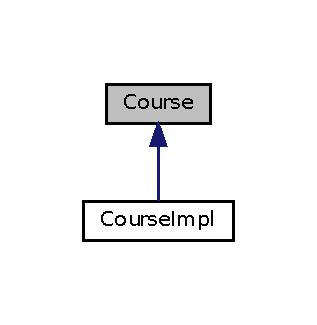
\includegraphics[width=152pt]{classCourse__inherit__graph}
\end{center}
\end{figure}
\subsection*{Public Member Functions}
\begin{DoxyCompactItemize}
\item 
virtual \hyperlink{classCourse_a80fed7c3f708fc4800517140cfbbb024}{$\sim$\+Course} ()
\begin{DoxyCompactList}\small\item\em Destroy the \hyperlink{classCourse}{Course} object. \end{DoxyCompactList}\item 
virtual string \hyperlink{classCourse_aaf464936166f94c89b97671798996088}{get\+Name} () const =0
\begin{DoxyCompactList}\small\item\em Get the Name object. \end{DoxyCompactList}\item 
virtual void \hyperlink{classCourse_abf95977e0ba0285c17cac6845f78c4e8}{set\+Name} (const string \&)=0
\begin{DoxyCompactList}\small\item\em Set the Name object. \end{DoxyCompactList}\item 
virtual string \hyperlink{classCourse_a19bced7786d959ca6110afc6d00bc751}{get\+Description} () const =0
\begin{DoxyCompactList}\small\item\em Get the Description object. \end{DoxyCompactList}\item 
virtual void \hyperlink{classCourse_a67f5badeddc228e5a4e4dde35f794d97}{set\+Description} (const string \&)=0
\begin{DoxyCompactList}\small\item\em Set the Description object. \end{DoxyCompactList}\item 
virtual string \hyperlink{classCourse_a7046438034cb468602eecf2c02013c00}{get\+Price} () const =0
\begin{DoxyCompactList}\small\item\em Get the Price object. \end{DoxyCompactList}\item 
virtual void \hyperlink{classCourse_a0a04b90e278236abbe5dbe40890cb3d0}{set\+Price} (const string \&)=0
\begin{DoxyCompactList}\small\item\em Set the Price object. \end{DoxyCompactList}\item 
virtual \hyperlink{classCourse}{Course} \& \hyperlink{classCourse_a460bb6c7b1acb7ecf6a702a3e890e32e}{operator=} (\hyperlink{classCourse}{Course} \&)=0
\begin{DoxyCompactList}\small\item\em assignment operator \end{DoxyCompactList}\end{DoxyCompactItemize}


\subsection{Detailed Description}
this class represents a course 

\subsection{Constructor \& Destructor Documentation}
\mbox{\Hypertarget{classCourse_a80fed7c3f708fc4800517140cfbbb024}\label{classCourse_a80fed7c3f708fc4800517140cfbbb024}} 
\index{Course@{Course}!````~Course@{$\sim$\+Course}}
\index{````~Course@{$\sim$\+Course}!Course@{Course}}
\subsubsection{\texorpdfstring{$\sim$\+Course()}{~Course()}}
{\footnotesize\ttfamily virtual Course\+::$\sim$\+Course (\begin{DoxyParamCaption}{ }\end{DoxyParamCaption})\hspace{0.3cm}{\ttfamily [inline]}, {\ttfamily [virtual]}}



Destroy the \hyperlink{classCourse}{Course} object. 



\subsection{Member Function Documentation}
\mbox{\Hypertarget{classCourse_a19bced7786d959ca6110afc6d00bc751}\label{classCourse_a19bced7786d959ca6110afc6d00bc751}} 
\index{Course@{Course}!get\+Description@{get\+Description}}
\index{get\+Description@{get\+Description}!Course@{Course}}
\subsubsection{\texorpdfstring{get\+Description()}{getDescription()}}
{\footnotesize\ttfamily virtual string Course\+::get\+Description (\begin{DoxyParamCaption}{ }\end{DoxyParamCaption}) const\hspace{0.3cm}{\ttfamily [pure virtual]}}



Get the Description object. 

\begin{DoxyReturn}{Returns}
string the \hyperlink{classCourse}{Course}\textquotesingle{}s description 
\end{DoxyReturn}


Implemented in \hyperlink{classCourseImpl_adff450841bfdf955061e01088d67f948}{Course\+Impl}.

\mbox{\Hypertarget{classCourse_aaf464936166f94c89b97671798996088}\label{classCourse_aaf464936166f94c89b97671798996088}} 
\index{Course@{Course}!get\+Name@{get\+Name}}
\index{get\+Name@{get\+Name}!Course@{Course}}
\subsubsection{\texorpdfstring{get\+Name()}{getName()}}
{\footnotesize\ttfamily virtual string Course\+::get\+Name (\begin{DoxyParamCaption}{ }\end{DoxyParamCaption}) const\hspace{0.3cm}{\ttfamily [pure virtual]}}



Get the Name object. 

\begin{DoxyReturn}{Returns}
string the \hyperlink{classCourse}{Course}\textquotesingle{}s name 
\end{DoxyReturn}


Implemented in \hyperlink{classCourseImpl_ab1f1244e63d4d2938f1640d7ef308319}{Course\+Impl}.

\mbox{\Hypertarget{classCourse_a7046438034cb468602eecf2c02013c00}\label{classCourse_a7046438034cb468602eecf2c02013c00}} 
\index{Course@{Course}!get\+Price@{get\+Price}}
\index{get\+Price@{get\+Price}!Course@{Course}}
\subsubsection{\texorpdfstring{get\+Price()}{getPrice()}}
{\footnotesize\ttfamily virtual string Course\+::get\+Price (\begin{DoxyParamCaption}{ }\end{DoxyParamCaption}) const\hspace{0.3cm}{\ttfamily [pure virtual]}}



Get the Price object. 

\begin{DoxyReturn}{Returns}
string the \hyperlink{classCourse}{Course}\textquotesingle{}s price 
\end{DoxyReturn}


Implemented in \hyperlink{classCourseImpl_a0b7ff83c24bd1d8e7a6d10b6b89883cd}{Course\+Impl}.

\mbox{\Hypertarget{classCourse_a460bb6c7b1acb7ecf6a702a3e890e32e}\label{classCourse_a460bb6c7b1acb7ecf6a702a3e890e32e}} 
\index{Course@{Course}!operator=@{operator=}}
\index{operator=@{operator=}!Course@{Course}}
\subsubsection{\texorpdfstring{operator=()}{operator=()}}
{\footnotesize\ttfamily virtual \hyperlink{classCourse}{Course}\& Course\+::operator= (\begin{DoxyParamCaption}\item[{\hyperlink{classCourse}{Course} \&}]{ }\end{DoxyParamCaption})\hspace{0.3cm}{\ttfamily [pure virtual]}}



assignment operator 

\begin{DoxyReturn}{Returns}
\hyperlink{classCourse}{Course}\& \hyperlink{classCourse}{Course} reference 
\end{DoxyReturn}


Implemented in \hyperlink{classCourseImpl_a2a35e597103c55fd43b68e78c76952e6}{Course\+Impl}.

\mbox{\Hypertarget{classCourse_a67f5badeddc228e5a4e4dde35f794d97}\label{classCourse_a67f5badeddc228e5a4e4dde35f794d97}} 
\index{Course@{Course}!set\+Description@{set\+Description}}
\index{set\+Description@{set\+Description}!Course@{Course}}
\subsubsection{\texorpdfstring{set\+Description()}{setDescription()}}
{\footnotesize\ttfamily virtual void Course\+::set\+Description (\begin{DoxyParamCaption}\item[{const string \&}]{ }\end{DoxyParamCaption})\hspace{0.3cm}{\ttfamily [pure virtual]}}



Set the Description object. 



Implemented in \hyperlink{classCourseImpl_a38d1a7f80f078828f9f2795aa4219e91}{Course\+Impl}.

\mbox{\Hypertarget{classCourse_abf95977e0ba0285c17cac6845f78c4e8}\label{classCourse_abf95977e0ba0285c17cac6845f78c4e8}} 
\index{Course@{Course}!set\+Name@{set\+Name}}
\index{set\+Name@{set\+Name}!Course@{Course}}
\subsubsection{\texorpdfstring{set\+Name()}{setName()}}
{\footnotesize\ttfamily virtual void Course\+::set\+Name (\begin{DoxyParamCaption}\item[{const string \&}]{ }\end{DoxyParamCaption})\hspace{0.3cm}{\ttfamily [pure virtual]}}



Set the Name object. 



Implemented in \hyperlink{classCourseImpl_af831a30978ba95ab38c90cb82d14ed7b}{Course\+Impl}.

\mbox{\Hypertarget{classCourse_a0a04b90e278236abbe5dbe40890cb3d0}\label{classCourse_a0a04b90e278236abbe5dbe40890cb3d0}} 
\index{Course@{Course}!set\+Price@{set\+Price}}
\index{set\+Price@{set\+Price}!Course@{Course}}
\subsubsection{\texorpdfstring{set\+Price()}{setPrice()}}
{\footnotesize\ttfamily virtual void Course\+::set\+Price (\begin{DoxyParamCaption}\item[{const string \&}]{ }\end{DoxyParamCaption})\hspace{0.3cm}{\ttfamily [pure virtual]}}



Set the Price object. 



Implemented in \hyperlink{classCourseImpl_a83623c7a5eff0d028151e4d2126884de}{Course\+Impl}.



The documentation for this class was generated from the following file\+:\begin{DoxyCompactItemize}
\item 
src/classes/\hyperlink{course_8h}{course.\+h}\end{DoxyCompactItemize}

\hypertarget{classCourseImpl}{}\section{Course\+Impl Class Reference}
\label{classCourseImpl}\index{Course\+Impl@{Course\+Impl}}


this represents a course  




{\ttfamily \#include $<$course\+\_\+impl.\+h$>$}



Inheritance diagram for Course\+Impl\+:
\nopagebreak
\begin{figure}[H]
\begin{center}
\leavevmode
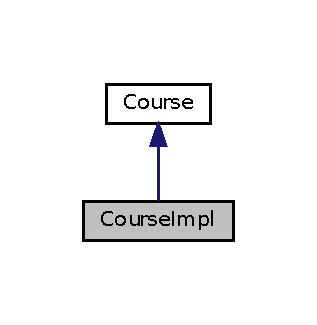
\includegraphics[width=152pt]{classCourseImpl__inherit__graph}
\end{center}
\end{figure}


Collaboration diagram for Course\+Impl\+:
\nopagebreak
\begin{figure}[H]
\begin{center}
\leavevmode
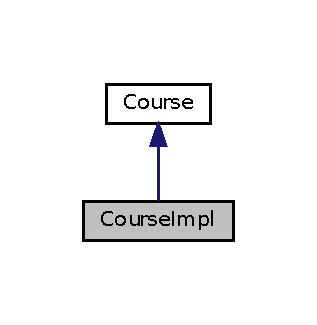
\includegraphics[width=152pt]{classCourseImpl__coll__graph}
\end{center}
\end{figure}
\subsection*{Public Member Functions}
\begin{DoxyCompactItemize}
\item 
\hyperlink{classCourseImpl_a1f90c3b1232d808f1adfd22700ae0c36}{Course\+Impl} ()
\begin{DoxyCompactList}\small\item\em Construct a new \hyperlink{classCourse}{Course} Impl object. \end{DoxyCompactList}\item 
\hyperlink{classCourseImpl_a2d4d21ad889d02d6ad25827fa7d87e59}{Course\+Impl} (\hyperlink{classCourse}{Course} $\ast$)
\begin{DoxyCompactList}\small\item\em Construct a new \hyperlink{classCourse}{Course} Impl object. \end{DoxyCompactList}\item 
\hyperlink{classCourseImpl_ad762665b174957dbdecd37945b52e41d}{Course\+Impl} (string, string, string)
\begin{DoxyCompactList}\small\item\em Construct a new \hyperlink{classCourse}{Course} Impl object. \end{DoxyCompactList}\item 
\hyperlink{classCourseImpl_a113b20eec8d5dbd8ce66e596ff467477}{$\sim$\+Course\+Impl} ()
\begin{DoxyCompactList}\small\item\em Destroy the \hyperlink{classCourse}{Course} Impl object. \end{DoxyCompactList}\item 
string \hyperlink{classCourseImpl_ab1f1244e63d4d2938f1640d7ef308319}{get\+Name} () const
\begin{DoxyCompactList}\small\item\em Get the Name object. \end{DoxyCompactList}\item 
void \hyperlink{classCourseImpl_af831a30978ba95ab38c90cb82d14ed7b}{set\+Name} (const string \&)
\begin{DoxyCompactList}\small\item\em Set the Name object. \end{DoxyCompactList}\item 
string \hyperlink{classCourseImpl_adff450841bfdf955061e01088d67f948}{get\+Description} () const
\begin{DoxyCompactList}\small\item\em Get the Description object. \end{DoxyCompactList}\item 
void \hyperlink{classCourseImpl_a38d1a7f80f078828f9f2795aa4219e91}{set\+Description} (const string \&)
\begin{DoxyCompactList}\small\item\em Set the Description object. \end{DoxyCompactList}\item 
string \hyperlink{classCourseImpl_a0b7ff83c24bd1d8e7a6d10b6b89883cd}{get\+Price} () const
\begin{DoxyCompactList}\small\item\em Get the Price object. \end{DoxyCompactList}\item 
void \hyperlink{classCourseImpl_a83623c7a5eff0d028151e4d2126884de}{set\+Price} (const string \&)
\begin{DoxyCompactList}\small\item\em Set the Price object. \end{DoxyCompactList}\item 
\hyperlink{classCourse}{Course} \& \hyperlink{classCourseImpl_a2a35e597103c55fd43b68e78c76952e6}{operator=} (\hyperlink{classCourse}{Course} \&)
\begin{DoxyCompactList}\small\item\em assignment operator \end{DoxyCompactList}\end{DoxyCompactItemize}
\subsection*{Protected Attributes}
\begin{DoxyCompactItemize}
\item 
string \hyperlink{classCourseImpl_a1889e262381ed6f13aa57ad116f050e7}{name}
\item 
string \hyperlink{classCourseImpl_aaf5d0d4c16bc2d0403f0baae29b7600c}{description}
\item 
string \hyperlink{classCourseImpl_a1599d100a1c5a01277e28e8777c03666}{price}
\end{DoxyCompactItemize}


\subsection{Detailed Description}
this represents a course 

\subsection{Constructor \& Destructor Documentation}
\mbox{\Hypertarget{classCourseImpl_a1f90c3b1232d808f1adfd22700ae0c36}\label{classCourseImpl_a1f90c3b1232d808f1adfd22700ae0c36}} 
\index{Course\+Impl@{Course\+Impl}!Course\+Impl@{Course\+Impl}}
\index{Course\+Impl@{Course\+Impl}!Course\+Impl@{Course\+Impl}}
\subsubsection{\texorpdfstring{Course\+Impl()}{CourseImpl()}\hspace{0.1cm}{\footnotesize\ttfamily [1/3]}}
{\footnotesize\ttfamily Course\+Impl\+::\+Course\+Impl (\begin{DoxyParamCaption}{ }\end{DoxyParamCaption})}



Construct a new \hyperlink{classCourse}{Course} Impl object. 

\mbox{\Hypertarget{classCourseImpl_a2d4d21ad889d02d6ad25827fa7d87e59}\label{classCourseImpl_a2d4d21ad889d02d6ad25827fa7d87e59}} 
\index{Course\+Impl@{Course\+Impl}!Course\+Impl@{Course\+Impl}}
\index{Course\+Impl@{Course\+Impl}!Course\+Impl@{Course\+Impl}}
\subsubsection{\texorpdfstring{Course\+Impl()}{CourseImpl()}\hspace{0.1cm}{\footnotesize\ttfamily [2/3]}}
{\footnotesize\ttfamily Course\+Impl\+::\+Course\+Impl (\begin{DoxyParamCaption}\item[{\hyperlink{classCourse}{Course} $\ast$}]{course }\end{DoxyParamCaption})}



Construct a new \hyperlink{classCourse}{Course} Impl object. 

\mbox{\Hypertarget{classCourseImpl_ad762665b174957dbdecd37945b52e41d}\label{classCourseImpl_ad762665b174957dbdecd37945b52e41d}} 
\index{Course\+Impl@{Course\+Impl}!Course\+Impl@{Course\+Impl}}
\index{Course\+Impl@{Course\+Impl}!Course\+Impl@{Course\+Impl}}
\subsubsection{\texorpdfstring{Course\+Impl()}{CourseImpl()}\hspace{0.1cm}{\footnotesize\ttfamily [3/3]}}
{\footnotesize\ttfamily Course\+Impl\+::\+Course\+Impl (\begin{DoxyParamCaption}\item[{string}]{name,  }\item[{string}]{description,  }\item[{string}]{price }\end{DoxyParamCaption})}



Construct a new \hyperlink{classCourse}{Course} Impl object. 

\mbox{\Hypertarget{classCourseImpl_a113b20eec8d5dbd8ce66e596ff467477}\label{classCourseImpl_a113b20eec8d5dbd8ce66e596ff467477}} 
\index{Course\+Impl@{Course\+Impl}!````~Course\+Impl@{$\sim$\+Course\+Impl}}
\index{````~Course\+Impl@{$\sim$\+Course\+Impl}!Course\+Impl@{Course\+Impl}}
\subsubsection{\texorpdfstring{$\sim$\+Course\+Impl()}{~CourseImpl()}}
{\footnotesize\ttfamily Course\+Impl\+::$\sim$\+Course\+Impl (\begin{DoxyParamCaption}{ }\end{DoxyParamCaption})}



Destroy the \hyperlink{classCourse}{Course} Impl object. 



\subsection{Member Function Documentation}
\mbox{\Hypertarget{classCourseImpl_adff450841bfdf955061e01088d67f948}\label{classCourseImpl_adff450841bfdf955061e01088d67f948}} 
\index{Course\+Impl@{Course\+Impl}!get\+Description@{get\+Description}}
\index{get\+Description@{get\+Description}!Course\+Impl@{Course\+Impl}}
\subsubsection{\texorpdfstring{get\+Description()}{getDescription()}}
{\footnotesize\ttfamily string Course\+Impl\+::get\+Description (\begin{DoxyParamCaption}{ }\end{DoxyParamCaption}) const\hspace{0.3cm}{\ttfamily [virtual]}}



Get the Description object. 

\begin{DoxyReturn}{Returns}
string the \hyperlink{classCourse}{Course}\textquotesingle{}s description 
\end{DoxyReturn}


Implements \hyperlink{classCourse_a19bced7786d959ca6110afc6d00bc751}{Course}.

\mbox{\Hypertarget{classCourseImpl_ab1f1244e63d4d2938f1640d7ef308319}\label{classCourseImpl_ab1f1244e63d4d2938f1640d7ef308319}} 
\index{Course\+Impl@{Course\+Impl}!get\+Name@{get\+Name}}
\index{get\+Name@{get\+Name}!Course\+Impl@{Course\+Impl}}
\subsubsection{\texorpdfstring{get\+Name()}{getName()}}
{\footnotesize\ttfamily string Course\+Impl\+::get\+Name (\begin{DoxyParamCaption}{ }\end{DoxyParamCaption}) const\hspace{0.3cm}{\ttfamily [virtual]}}



Get the Name object. 

\begin{DoxyReturn}{Returns}
string the \hyperlink{classCourse}{Course}\textquotesingle{}s name 
\end{DoxyReturn}


Implements \hyperlink{classCourse_aaf464936166f94c89b97671798996088}{Course}.

\mbox{\Hypertarget{classCourseImpl_a0b7ff83c24bd1d8e7a6d10b6b89883cd}\label{classCourseImpl_a0b7ff83c24bd1d8e7a6d10b6b89883cd}} 
\index{Course\+Impl@{Course\+Impl}!get\+Price@{get\+Price}}
\index{get\+Price@{get\+Price}!Course\+Impl@{Course\+Impl}}
\subsubsection{\texorpdfstring{get\+Price()}{getPrice()}}
{\footnotesize\ttfamily string Course\+Impl\+::get\+Price (\begin{DoxyParamCaption}{ }\end{DoxyParamCaption}) const\hspace{0.3cm}{\ttfamily [virtual]}}



Get the Price object. 

\begin{DoxyReturn}{Returns}
string the \hyperlink{classCourse}{Course}\textquotesingle{}s price 
\end{DoxyReturn}


Implements \hyperlink{classCourse_a7046438034cb468602eecf2c02013c00}{Course}.

\mbox{\Hypertarget{classCourseImpl_a2a35e597103c55fd43b68e78c76952e6}\label{classCourseImpl_a2a35e597103c55fd43b68e78c76952e6}} 
\index{Course\+Impl@{Course\+Impl}!operator=@{operator=}}
\index{operator=@{operator=}!Course\+Impl@{Course\+Impl}}
\subsubsection{\texorpdfstring{operator=()}{operator=()}}
{\footnotesize\ttfamily \hyperlink{classCourse}{Course} \& Course\+Impl\+::operator= (\begin{DoxyParamCaption}\item[{\hyperlink{classCourse}{Course} \&}]{course }\end{DoxyParamCaption})\hspace{0.3cm}{\ttfamily [virtual]}}



assignment operator 

\begin{DoxyReturn}{Returns}
\hyperlink{classCourse}{Course}\& \hyperlink{classCourse}{Course} reference 
\end{DoxyReturn}


Implements \hyperlink{classCourse_a460bb6c7b1acb7ecf6a702a3e890e32e}{Course}.

\mbox{\Hypertarget{classCourseImpl_a38d1a7f80f078828f9f2795aa4219e91}\label{classCourseImpl_a38d1a7f80f078828f9f2795aa4219e91}} 
\index{Course\+Impl@{Course\+Impl}!set\+Description@{set\+Description}}
\index{set\+Description@{set\+Description}!Course\+Impl@{Course\+Impl}}
\subsubsection{\texorpdfstring{set\+Description()}{setDescription()}}
{\footnotesize\ttfamily void Course\+Impl\+::set\+Description (\begin{DoxyParamCaption}\item[{const string \&}]{description }\end{DoxyParamCaption})\hspace{0.3cm}{\ttfamily [virtual]}}



Set the Description object. 



Implements \hyperlink{classCourse_a67f5badeddc228e5a4e4dde35f794d97}{Course}.

\mbox{\Hypertarget{classCourseImpl_af831a30978ba95ab38c90cb82d14ed7b}\label{classCourseImpl_af831a30978ba95ab38c90cb82d14ed7b}} 
\index{Course\+Impl@{Course\+Impl}!set\+Name@{set\+Name}}
\index{set\+Name@{set\+Name}!Course\+Impl@{Course\+Impl}}
\subsubsection{\texorpdfstring{set\+Name()}{setName()}}
{\footnotesize\ttfamily void Course\+Impl\+::set\+Name (\begin{DoxyParamCaption}\item[{const string \&}]{name }\end{DoxyParamCaption})\hspace{0.3cm}{\ttfamily [virtual]}}



Set the Name object. 



Implements \hyperlink{classCourse_abf95977e0ba0285c17cac6845f78c4e8}{Course}.

\mbox{\Hypertarget{classCourseImpl_a83623c7a5eff0d028151e4d2126884de}\label{classCourseImpl_a83623c7a5eff0d028151e4d2126884de}} 
\index{Course\+Impl@{Course\+Impl}!set\+Price@{set\+Price}}
\index{set\+Price@{set\+Price}!Course\+Impl@{Course\+Impl}}
\subsubsection{\texorpdfstring{set\+Price()}{setPrice()}}
{\footnotesize\ttfamily void Course\+Impl\+::set\+Price (\begin{DoxyParamCaption}\item[{const string \&}]{price }\end{DoxyParamCaption})\hspace{0.3cm}{\ttfamily [virtual]}}



Set the Price object. 



Implements \hyperlink{classCourse_a0a04b90e278236abbe5dbe40890cb3d0}{Course}.



\subsection{Member Data Documentation}
\mbox{\Hypertarget{classCourseImpl_aaf5d0d4c16bc2d0403f0baae29b7600c}\label{classCourseImpl_aaf5d0d4c16bc2d0403f0baae29b7600c}} 
\index{Course\+Impl@{Course\+Impl}!description@{description}}
\index{description@{description}!Course\+Impl@{Course\+Impl}}
\subsubsection{\texorpdfstring{description}{description}}
{\footnotesize\ttfamily string Course\+Impl\+::description\hspace{0.3cm}{\ttfamily [protected]}}

\mbox{\Hypertarget{classCourseImpl_a1889e262381ed6f13aa57ad116f050e7}\label{classCourseImpl_a1889e262381ed6f13aa57ad116f050e7}} 
\index{Course\+Impl@{Course\+Impl}!name@{name}}
\index{name@{name}!Course\+Impl@{Course\+Impl}}
\subsubsection{\texorpdfstring{name}{name}}
{\footnotesize\ttfamily string Course\+Impl\+::name\hspace{0.3cm}{\ttfamily [protected]}}

\mbox{\Hypertarget{classCourseImpl_a1599d100a1c5a01277e28e8777c03666}\label{classCourseImpl_a1599d100a1c5a01277e28e8777c03666}} 
\index{Course\+Impl@{Course\+Impl}!price@{price}}
\index{price@{price}!Course\+Impl@{Course\+Impl}}
\subsubsection{\texorpdfstring{price}{price}}
{\footnotesize\ttfamily string Course\+Impl\+::price\hspace{0.3cm}{\ttfamily [protected]}}



The documentation for this class was generated from the following files\+:\begin{DoxyCompactItemize}
\item 
src/classes/\hyperlink{course__impl_8h}{course\+\_\+impl.\+h}\item 
src/classes/\hyperlink{course__impl_8cpp}{course\+\_\+impl.\+cpp}\end{DoxyCompactItemize}

\hypertarget{classeditclient}{}\section{editclient Class Reference}
\label{classeditclient}\index{editclient@{editclient}}


This class represents the page to edit the user\textquotesingle{}s values.  




{\ttfamily \#include $<$editclient.\+h$>$}



Inheritance diagram for editclient\+:\nopagebreak
\begin{figure}[H]
\begin{center}
\leavevmode
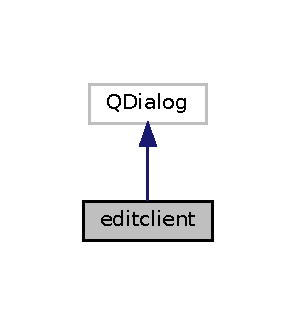
\includegraphics[width=142pt]{classeditclient__inherit__graph}
\end{center}
\end{figure}


Collaboration diagram for editclient\+:\nopagebreak
\begin{figure}[H]
\begin{center}
\leavevmode
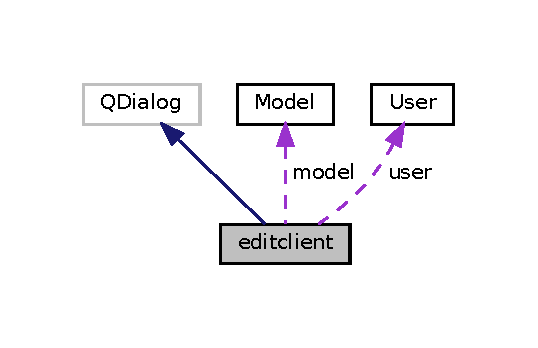
\includegraphics[width=258pt]{classeditclient__coll__graph}
\end{center}
\end{figure}
\subsection*{Public Member Functions}
\begin{DoxyCompactItemize}
\item 
\hyperlink{classeditclient_a5ea13813becddce68bcda899fbf7bad1}{editclient} (Q\+Widget $\ast$parent=nullptr)
\begin{DoxyCompactList}\small\item\em Construct a new editclient object. \end{DoxyCompactList}\item 
\hyperlink{classeditclient_ac881d2dd9b89bfec7632f85efe967d21}{$\sim$editclient} ()
\begin{DoxyCompactList}\small\item\em Destroy the editclient object. \end{DoxyCompactList}\item 
\hyperlink{classUser}{User} $\ast$ \hyperlink{classeditclient_ae9f2a67e859a01828e321ef86631afaf}{get\+User} () const
\begin{DoxyCompactList}\small\item\em Get the \hyperlink{classUser}{User} object. \end{DoxyCompactList}\item 
void \hyperlink{classeditclient_acc61aaf32845af5f061c565e15ee14cc}{set\+User} (\hyperlink{classUser}{User} $\ast$value)
\begin{DoxyCompactList}\small\item\em Set the \hyperlink{classUser}{User} object. \end{DoxyCompactList}\item 
\hyperlink{classModel}{Model} $\ast$ \hyperlink{classeditclient_a134cd4aaa1c6dcef1a1c4455569bf51d}{get\+Model} () const
\begin{DoxyCompactList}\small\item\em Get the \hyperlink{classModel}{Model} object. \end{DoxyCompactList}\item 
void \hyperlink{classeditclient_a70e9ccebb55d8683339c90eb2eef1107}{set\+Model} (\hyperlink{classModel}{Model} $\ast$value)
\begin{DoxyCompactList}\small\item\em Set the \hyperlink{classModel}{Model} object. \end{DoxyCompactList}\end{DoxyCompactItemize}
\subsection*{Private Slots}
\begin{DoxyCompactItemize}
\item 
void \hyperlink{classeditclient_af544394137d9de69e4890e2ecac7fb6a}{on\+\_\+cancel\+\_\+btn\+\_\+edit\+\_\+client\+\_\+clicked} ()
\begin{DoxyCompactList}\small\item\em function to cancel the update \end{DoxyCompactList}\item 
void \hyperlink{classeditclient_ab693a42ef8626fc5c856b69b8dcf4e35}{on\+\_\+update\+\_\+btn\+\_\+clicked} ()
\begin{DoxyCompactList}\small\item\em function to update profile \end{DoxyCompactList}\item 
void \hyperlink{classeditclient_aecd65327aeb31a9bf7ba282ae3d35303}{on\+\_\+remove\+\_\+profile\+\_\+btn\+\_\+clicked} ()
\begin{DoxyCompactList}\small\item\em function to remove profile \end{DoxyCompactList}\end{DoxyCompactItemize}
\subsection*{Private Attributes}
\begin{DoxyCompactItemize}
\item 
Ui\+::editclient $\ast$ \hyperlink{classeditclient_a675352f4a557aec3af37bd4fb5dfea60}{ui}
\item 
\hyperlink{classModel}{Model} $\ast$ \hyperlink{classeditclient_aaaf4f3349486a47f6e3a1ced0d5dcd64}{model}
\item 
\hyperlink{classUser}{User} $\ast$ \hyperlink{classeditclient_a5945bbf29ac9a75c8a680f6623460899}{user}
\end{DoxyCompactItemize}


\subsection{Detailed Description}
This class represents the page to edit the user\textquotesingle{}s values. 

\subsection{Constructor \& Destructor Documentation}
\mbox{\Hypertarget{classeditclient_a5ea13813becddce68bcda899fbf7bad1}\label{classeditclient_a5ea13813becddce68bcda899fbf7bad1}} 
\index{editclient@{editclient}!editclient@{editclient}}
\index{editclient@{editclient}!editclient@{editclient}}
\subsubsection{\texorpdfstring{editclient()}{editclient()}}
{\footnotesize\ttfamily editclient\+::editclient (\begin{DoxyParamCaption}\item[{Q\+Widget $\ast$}]{parent = {\ttfamily nullptr} }\end{DoxyParamCaption})\hspace{0.3cm}{\ttfamily [explicit]}}



Construct a new editclient object. 


\begin{DoxyParams}{Parameters}
{\em parent} & \\
\hline
\end{DoxyParams}
\mbox{\Hypertarget{classeditclient_ac881d2dd9b89bfec7632f85efe967d21}\label{classeditclient_ac881d2dd9b89bfec7632f85efe967d21}} 
\index{editclient@{editclient}!````~editclient@{$\sim$editclient}}
\index{````~editclient@{$\sim$editclient}!editclient@{editclient}}
\subsubsection{\texorpdfstring{$\sim$editclient()}{~editclient()}}
{\footnotesize\ttfamily editclient\+::$\sim$editclient (\begin{DoxyParamCaption}{ }\end{DoxyParamCaption})}



Destroy the editclient object. 



\subsection{Member Function Documentation}
\mbox{\Hypertarget{classeditclient_a134cd4aaa1c6dcef1a1c4455569bf51d}\label{classeditclient_a134cd4aaa1c6dcef1a1c4455569bf51d}} 
\index{editclient@{editclient}!get\+Model@{get\+Model}}
\index{get\+Model@{get\+Model}!editclient@{editclient}}
\subsubsection{\texorpdfstring{get\+Model()}{getModel()}}
{\footnotesize\ttfamily \hyperlink{classModel}{Model} $\ast$ editclient\+::get\+Model (\begin{DoxyParamCaption}{ }\end{DoxyParamCaption}) const}



Get the \hyperlink{classModel}{Model} object. 

\begin{DoxyReturn}{Returns}
Model$\ast$ the Edit Client\textquotesingle{}s model 
\end{DoxyReturn}
\mbox{\Hypertarget{classeditclient_ae9f2a67e859a01828e321ef86631afaf}\label{classeditclient_ae9f2a67e859a01828e321ef86631afaf}} 
\index{editclient@{editclient}!get\+User@{get\+User}}
\index{get\+User@{get\+User}!editclient@{editclient}}
\subsubsection{\texorpdfstring{get\+User()}{getUser()}}
{\footnotesize\ttfamily \hyperlink{classUser}{User} $\ast$ editclient\+::get\+User (\begin{DoxyParamCaption}{ }\end{DoxyParamCaption}) const}



Get the \hyperlink{classUser}{User} object. 

\begin{DoxyReturn}{Returns}
User$\ast$ the \hyperlink{classUser}{User} to be updated 
\end{DoxyReturn}
\mbox{\Hypertarget{classeditclient_af544394137d9de69e4890e2ecac7fb6a}\label{classeditclient_af544394137d9de69e4890e2ecac7fb6a}} 
\index{editclient@{editclient}!on\+\_\+cancel\+\_\+btn\+\_\+edit\+\_\+client\+\_\+clicked@{on\+\_\+cancel\+\_\+btn\+\_\+edit\+\_\+client\+\_\+clicked}}
\index{on\+\_\+cancel\+\_\+btn\+\_\+edit\+\_\+client\+\_\+clicked@{on\+\_\+cancel\+\_\+btn\+\_\+edit\+\_\+client\+\_\+clicked}!editclient@{editclient}}
\subsubsection{\texorpdfstring{on\+\_\+cancel\+\_\+btn\+\_\+edit\+\_\+client\+\_\+clicked}{on\_cancel\_btn\_edit\_client\_clicked}}
{\footnotesize\ttfamily void editclient\+::on\+\_\+cancel\+\_\+btn\+\_\+edit\+\_\+client\+\_\+clicked (\begin{DoxyParamCaption}{ }\end{DoxyParamCaption})\hspace{0.3cm}{\ttfamily [private]}, {\ttfamily [slot]}}



function to cancel the update 

\mbox{\Hypertarget{classeditclient_aecd65327aeb31a9bf7ba282ae3d35303}\label{classeditclient_aecd65327aeb31a9bf7ba282ae3d35303}} 
\index{editclient@{editclient}!on\+\_\+remove\+\_\+profile\+\_\+btn\+\_\+clicked@{on\+\_\+remove\+\_\+profile\+\_\+btn\+\_\+clicked}}
\index{on\+\_\+remove\+\_\+profile\+\_\+btn\+\_\+clicked@{on\+\_\+remove\+\_\+profile\+\_\+btn\+\_\+clicked}!editclient@{editclient}}
\subsubsection{\texorpdfstring{on\+\_\+remove\+\_\+profile\+\_\+btn\+\_\+clicked}{on\_remove\_profile\_btn\_clicked}}
{\footnotesize\ttfamily void editclient\+::on\+\_\+remove\+\_\+profile\+\_\+btn\+\_\+clicked (\begin{DoxyParamCaption}{ }\end{DoxyParamCaption})\hspace{0.3cm}{\ttfamily [private]}, {\ttfamily [slot]}}



function to remove profile 

\mbox{\Hypertarget{classeditclient_ab693a42ef8626fc5c856b69b8dcf4e35}\label{classeditclient_ab693a42ef8626fc5c856b69b8dcf4e35}} 
\index{editclient@{editclient}!on\+\_\+update\+\_\+btn\+\_\+clicked@{on\+\_\+update\+\_\+btn\+\_\+clicked}}
\index{on\+\_\+update\+\_\+btn\+\_\+clicked@{on\+\_\+update\+\_\+btn\+\_\+clicked}!editclient@{editclient}}
\subsubsection{\texorpdfstring{on\+\_\+update\+\_\+btn\+\_\+clicked}{on\_update\_btn\_clicked}}
{\footnotesize\ttfamily void editclient\+::on\+\_\+update\+\_\+btn\+\_\+clicked (\begin{DoxyParamCaption}{ }\end{DoxyParamCaption})\hspace{0.3cm}{\ttfamily [private]}, {\ttfamily [slot]}}



function to update profile 

\mbox{\Hypertarget{classeditclient_a70e9ccebb55d8683339c90eb2eef1107}\label{classeditclient_a70e9ccebb55d8683339c90eb2eef1107}} 
\index{editclient@{editclient}!set\+Model@{set\+Model}}
\index{set\+Model@{set\+Model}!editclient@{editclient}}
\subsubsection{\texorpdfstring{set\+Model()}{setModel()}}
{\footnotesize\ttfamily void editclient\+::set\+Model (\begin{DoxyParamCaption}\item[{\hyperlink{classModel}{Model} $\ast$}]{value }\end{DoxyParamCaption})}



Set the \hyperlink{classModel}{Model} object. 


\begin{DoxyParams}{Parameters}
{\em value} & the new Edit Client\textquotesingle{}s model \\
\hline
\end{DoxyParams}
\mbox{\Hypertarget{classeditclient_acc61aaf32845af5f061c565e15ee14cc}\label{classeditclient_acc61aaf32845af5f061c565e15ee14cc}} 
\index{editclient@{editclient}!set\+User@{set\+User}}
\index{set\+User@{set\+User}!editclient@{editclient}}
\subsubsection{\texorpdfstring{set\+User()}{setUser()}}
{\footnotesize\ttfamily void editclient\+::set\+User (\begin{DoxyParamCaption}\item[{\hyperlink{classUser}{User} $\ast$}]{value }\end{DoxyParamCaption})}



Set the \hyperlink{classUser}{User} object. 


\begin{DoxyParams}{Parameters}
{\em value} & the \hyperlink{classUser}{User} to be updated \\
\hline
\end{DoxyParams}


\subsection{Member Data Documentation}
\mbox{\Hypertarget{classeditclient_aaaf4f3349486a47f6e3a1ced0d5dcd64}\label{classeditclient_aaaf4f3349486a47f6e3a1ced0d5dcd64}} 
\index{editclient@{editclient}!model@{model}}
\index{model@{model}!editclient@{editclient}}
\subsubsection{\texorpdfstring{model}{model}}
{\footnotesize\ttfamily \hyperlink{classModel}{Model}$\ast$ editclient\+::model\hspace{0.3cm}{\ttfamily [private]}}

\mbox{\Hypertarget{classeditclient_a675352f4a557aec3af37bd4fb5dfea60}\label{classeditclient_a675352f4a557aec3af37bd4fb5dfea60}} 
\index{editclient@{editclient}!ui@{ui}}
\index{ui@{ui}!editclient@{editclient}}
\subsubsection{\texorpdfstring{ui}{ui}}
{\footnotesize\ttfamily Ui\+::editclient$\ast$ editclient\+::ui\hspace{0.3cm}{\ttfamily [private]}}

\mbox{\Hypertarget{classeditclient_a5945bbf29ac9a75c8a680f6623460899}\label{classeditclient_a5945bbf29ac9a75c8a680f6623460899}} 
\index{editclient@{editclient}!user@{user}}
\index{user@{user}!editclient@{editclient}}
\subsubsection{\texorpdfstring{user}{user}}
{\footnotesize\ttfamily \hyperlink{classUser}{User}$\ast$ editclient\+::user\hspace{0.3cm}{\ttfamily [private]}}



The documentation for this class was generated from the following files\+:\begin{DoxyCompactItemize}
\item 
views/\hyperlink{editclient_8h}{editclient.\+h}\item 
views/\hyperlink{editclient_8cpp}{editclient.\+cpp}\end{DoxyCompactItemize}

\hypertarget{classEditCourse}{}\section{Edit\+Course Class Reference}
\label{classEditCourse}\index{Edit\+Course@{Edit\+Course}}


This class represents the page to edit the course\textquotesingle{}s values.  




{\ttfamily \#include $<$editcourse.\+h$>$}



Inheritance diagram for Edit\+Course\+:
\nopagebreak
\begin{figure}[H]
\begin{center}
\leavevmode
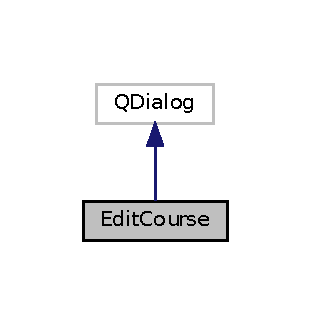
\includegraphics[width=149pt]{classEditCourse__inherit__graph}
\end{center}
\end{figure}


Collaboration diagram for Edit\+Course\+:
\nopagebreak
\begin{figure}[H]
\begin{center}
\leavevmode
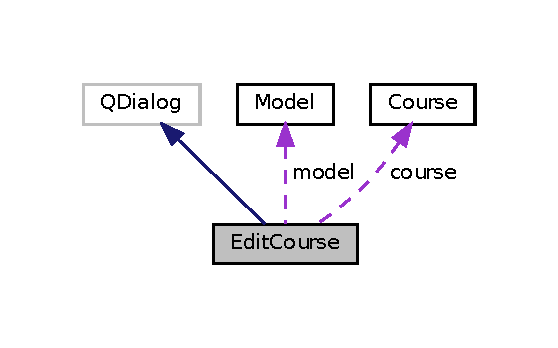
\includegraphics[width=268pt]{classEditCourse__coll__graph}
\end{center}
\end{figure}
\subsection*{Public Member Functions}
\begin{DoxyCompactItemize}
\item 
\hyperlink{classEditCourse_a9ef9057273412ffc11c923812781a817}{Edit\+Course} (Q\+Widget $\ast$parent=nullptr)
\begin{DoxyCompactList}\small\item\em Construct a new Edit \hyperlink{classCourse}{Course} object. \end{DoxyCompactList}\item 
\hyperlink{classEditCourse_a2820ede4b925099e088e288a48825485}{$\sim$\+Edit\+Course} ()
\begin{DoxyCompactList}\small\item\em Destroy the Edit \hyperlink{classCourse}{Course} object. \end{DoxyCompactList}\item 
\hyperlink{classCourse}{Course} $\ast$ \hyperlink{classEditCourse_a7e3f0d830ad339eab414d7fed354b4d9}{get\+Course} () const
\begin{DoxyCompactList}\small\item\em Get the \hyperlink{classCourse}{Course} object. \end{DoxyCompactList}\item 
void \hyperlink{classEditCourse_a263030185cb0d1f790b66be18cef630f}{set\+Course} (\hyperlink{classCourse}{Course} $\ast$value)
\begin{DoxyCompactList}\small\item\em Set the \hyperlink{classCourse}{Course} object. \end{DoxyCompactList}\item 
\hyperlink{classModel}{Model} $\ast$ \hyperlink{classEditCourse_a6c26566b7caaf2f44192bfc47b71212d}{get\+Model} () const
\begin{DoxyCompactList}\small\item\em Get the \hyperlink{classModel}{Model} object. \end{DoxyCompactList}\item 
void \hyperlink{classEditCourse_a055cf5be8cfb3e5af3910876e8285d98}{set\+Model} (\hyperlink{classModel}{Model} $\ast$value)
\begin{DoxyCompactList}\small\item\em Set the \hyperlink{classModel}{Model} object. \end{DoxyCompactList}\end{DoxyCompactItemize}
\subsection*{Private Slots}
\begin{DoxyCompactItemize}
\item 
void \hyperlink{classEditCourse_ae625c52f7558677c52ad62face57d349}{on\+\_\+edit\+\_\+btn\+\_\+clicked} ()
\begin{DoxyCompactList}\small\item\em function to updated the course\textquotesingle{}s values \end{DoxyCompactList}\item 
void \hyperlink{classEditCourse_a8cea0aa3e8f43d6a9aa3260e97e7713e}{on\+\_\+\+C\+A\+N\+C\+E\+L\+\_\+clicked} ()
\begin{DoxyCompactList}\small\item\em function to cancel the update \end{DoxyCompactList}\end{DoxyCompactItemize}
\subsection*{Private Attributes}
\begin{DoxyCompactItemize}
\item 
Ui\+::\+Edit\+Course $\ast$ \hyperlink{classEditCourse_a22a699a4ebce678c8837e9ae4f0aeed2}{ui}
\item 
\hyperlink{classModel}{Model} $\ast$ \hyperlink{classEditCourse_a7dfc909dd668bd50ba3653f7a8d77d34}{model}
\item 
\hyperlink{classCourse}{Course} $\ast$ \hyperlink{classEditCourse_af20120b1d0fe619456bf49b23002c3a1}{course}
\end{DoxyCompactItemize}


\subsection{Detailed Description}
This class represents the page to edit the course\textquotesingle{}s values. 

\subsection{Constructor \& Destructor Documentation}
\mbox{\Hypertarget{classEditCourse_a9ef9057273412ffc11c923812781a817}\label{classEditCourse_a9ef9057273412ffc11c923812781a817}} 
\index{Edit\+Course@{Edit\+Course}!Edit\+Course@{Edit\+Course}}
\index{Edit\+Course@{Edit\+Course}!Edit\+Course@{Edit\+Course}}
\subsubsection{\texorpdfstring{Edit\+Course()}{EditCourse()}}
{\footnotesize\ttfamily Edit\+Course\+::\+Edit\+Course (\begin{DoxyParamCaption}\item[{Q\+Widget $\ast$}]{parent = {\ttfamily nullptr} }\end{DoxyParamCaption})\hspace{0.3cm}{\ttfamily [explicit]}}



Construct a new Edit \hyperlink{classCourse}{Course} object. 


\begin{DoxyParams}{Parameters}
{\em parent} & \\
\hline
\end{DoxyParams}
\mbox{\Hypertarget{classEditCourse_a2820ede4b925099e088e288a48825485}\label{classEditCourse_a2820ede4b925099e088e288a48825485}} 
\index{Edit\+Course@{Edit\+Course}!````~Edit\+Course@{$\sim$\+Edit\+Course}}
\index{````~Edit\+Course@{$\sim$\+Edit\+Course}!Edit\+Course@{Edit\+Course}}
\subsubsection{\texorpdfstring{$\sim$\+Edit\+Course()}{~EditCourse()}}
{\footnotesize\ttfamily Edit\+Course\+::$\sim$\+Edit\+Course (\begin{DoxyParamCaption}{ }\end{DoxyParamCaption})}



Destroy the Edit \hyperlink{classCourse}{Course} object. 



\subsection{Member Function Documentation}
\mbox{\Hypertarget{classEditCourse_a7e3f0d830ad339eab414d7fed354b4d9}\label{classEditCourse_a7e3f0d830ad339eab414d7fed354b4d9}} 
\index{Edit\+Course@{Edit\+Course}!get\+Course@{get\+Course}}
\index{get\+Course@{get\+Course}!Edit\+Course@{Edit\+Course}}
\subsubsection{\texorpdfstring{get\+Course()}{getCourse()}}
{\footnotesize\ttfamily \hyperlink{classCourse}{Course} $\ast$ Edit\+Course\+::get\+Course (\begin{DoxyParamCaption}{ }\end{DoxyParamCaption}) const}



Get the \hyperlink{classCourse}{Course} object. 

\begin{DoxyReturn}{Returns}
Course$\ast$ the \hyperlink{classCourse}{Course} to be updated 
\end{DoxyReturn}
\mbox{\Hypertarget{classEditCourse_a6c26566b7caaf2f44192bfc47b71212d}\label{classEditCourse_a6c26566b7caaf2f44192bfc47b71212d}} 
\index{Edit\+Course@{Edit\+Course}!get\+Model@{get\+Model}}
\index{get\+Model@{get\+Model}!Edit\+Course@{Edit\+Course}}
\subsubsection{\texorpdfstring{get\+Model()}{getModel()}}
{\footnotesize\ttfamily \hyperlink{classModel}{Model} $\ast$ Edit\+Course\+::get\+Model (\begin{DoxyParamCaption}{ }\end{DoxyParamCaption}) const}



Get the \hyperlink{classModel}{Model} object. 

\begin{DoxyReturn}{Returns}
Model$\ast$ the Edit \hyperlink{classCourse}{Course}\textquotesingle{}s model 
\end{DoxyReturn}
\mbox{\Hypertarget{classEditCourse_a8cea0aa3e8f43d6a9aa3260e97e7713e}\label{classEditCourse_a8cea0aa3e8f43d6a9aa3260e97e7713e}} 
\index{Edit\+Course@{Edit\+Course}!on\+\_\+\+C\+A\+N\+C\+E\+L\+\_\+clicked@{on\+\_\+\+C\+A\+N\+C\+E\+L\+\_\+clicked}}
\index{on\+\_\+\+C\+A\+N\+C\+E\+L\+\_\+clicked@{on\+\_\+\+C\+A\+N\+C\+E\+L\+\_\+clicked}!Edit\+Course@{Edit\+Course}}
\subsubsection{\texorpdfstring{on\+\_\+\+C\+A\+N\+C\+E\+L\+\_\+clicked}{on\_CANCEL\_clicked}}
{\footnotesize\ttfamily void Edit\+Course\+::on\+\_\+\+C\+A\+N\+C\+E\+L\+\_\+clicked (\begin{DoxyParamCaption}{ }\end{DoxyParamCaption})\hspace{0.3cm}{\ttfamily [private]}, {\ttfamily [slot]}}



function to cancel the update 

\mbox{\Hypertarget{classEditCourse_ae625c52f7558677c52ad62face57d349}\label{classEditCourse_ae625c52f7558677c52ad62face57d349}} 
\index{Edit\+Course@{Edit\+Course}!on\+\_\+edit\+\_\+btn\+\_\+clicked@{on\+\_\+edit\+\_\+btn\+\_\+clicked}}
\index{on\+\_\+edit\+\_\+btn\+\_\+clicked@{on\+\_\+edit\+\_\+btn\+\_\+clicked}!Edit\+Course@{Edit\+Course}}
\subsubsection{\texorpdfstring{on\+\_\+edit\+\_\+btn\+\_\+clicked}{on\_edit\_btn\_clicked}}
{\footnotesize\ttfamily void Edit\+Course\+::on\+\_\+edit\+\_\+btn\+\_\+clicked (\begin{DoxyParamCaption}{ }\end{DoxyParamCaption})\hspace{0.3cm}{\ttfamily [private]}, {\ttfamily [slot]}}



function to updated the course\textquotesingle{}s values 

\mbox{\Hypertarget{classEditCourse_a263030185cb0d1f790b66be18cef630f}\label{classEditCourse_a263030185cb0d1f790b66be18cef630f}} 
\index{Edit\+Course@{Edit\+Course}!set\+Course@{set\+Course}}
\index{set\+Course@{set\+Course}!Edit\+Course@{Edit\+Course}}
\subsubsection{\texorpdfstring{set\+Course()}{setCourse()}}
{\footnotesize\ttfamily void Edit\+Course\+::set\+Course (\begin{DoxyParamCaption}\item[{\hyperlink{classCourse}{Course} $\ast$}]{value }\end{DoxyParamCaption})}



Set the \hyperlink{classCourse}{Course} object. 


\begin{DoxyParams}{Parameters}
{\em value} & the new \hyperlink{classCourse}{Course} to be updated \\
\hline
\end{DoxyParams}
\mbox{\Hypertarget{classEditCourse_a055cf5be8cfb3e5af3910876e8285d98}\label{classEditCourse_a055cf5be8cfb3e5af3910876e8285d98}} 
\index{Edit\+Course@{Edit\+Course}!set\+Model@{set\+Model}}
\index{set\+Model@{set\+Model}!Edit\+Course@{Edit\+Course}}
\subsubsection{\texorpdfstring{set\+Model()}{setModel()}}
{\footnotesize\ttfamily void Edit\+Course\+::set\+Model (\begin{DoxyParamCaption}\item[{\hyperlink{classModel}{Model} $\ast$}]{value }\end{DoxyParamCaption})}



Set the \hyperlink{classModel}{Model} object. 


\begin{DoxyParams}{Parameters}
{\em value} & the Edit \hyperlink{classCourse}{Course}\textquotesingle{}s new model \\
\hline
\end{DoxyParams}


\subsection{Member Data Documentation}
\mbox{\Hypertarget{classEditCourse_af20120b1d0fe619456bf49b23002c3a1}\label{classEditCourse_af20120b1d0fe619456bf49b23002c3a1}} 
\index{Edit\+Course@{Edit\+Course}!course@{course}}
\index{course@{course}!Edit\+Course@{Edit\+Course}}
\subsubsection{\texorpdfstring{course}{course}}
{\footnotesize\ttfamily \hyperlink{classCourse}{Course}$\ast$ Edit\+Course\+::course\hspace{0.3cm}{\ttfamily [private]}}

\mbox{\Hypertarget{classEditCourse_a7dfc909dd668bd50ba3653f7a8d77d34}\label{classEditCourse_a7dfc909dd668bd50ba3653f7a8d77d34}} 
\index{Edit\+Course@{Edit\+Course}!model@{model}}
\index{model@{model}!Edit\+Course@{Edit\+Course}}
\subsubsection{\texorpdfstring{model}{model}}
{\footnotesize\ttfamily \hyperlink{classModel}{Model}$\ast$ Edit\+Course\+::model\hspace{0.3cm}{\ttfamily [private]}}

\mbox{\Hypertarget{classEditCourse_a22a699a4ebce678c8837e9ae4f0aeed2}\label{classEditCourse_a22a699a4ebce678c8837e9ae4f0aeed2}} 
\index{Edit\+Course@{Edit\+Course}!ui@{ui}}
\index{ui@{ui}!Edit\+Course@{Edit\+Course}}
\subsubsection{\texorpdfstring{ui}{ui}}
{\footnotesize\ttfamily Ui\+::\+Edit\+Course$\ast$ Edit\+Course\+::ui\hspace{0.3cm}{\ttfamily [private]}}



The documentation for this class was generated from the following files\+:\begin{DoxyCompactItemize}
\item 
views/\hyperlink{editcourse_8h}{editcourse.\+h}\item 
views/\hyperlink{editcourse_8cpp}{editcourse.\+cpp}\end{DoxyCompactItemize}

\hypertarget{classlogin}{}\section{login Class Reference}
\label{classlogin}\index{login@{login}}


this class representer a Login UI  




{\ttfamily \#include $<$login.\+h$>$}



Inheritance diagram for login\+:
\nopagebreak
\begin{figure}[H]
\begin{center}
\leavevmode
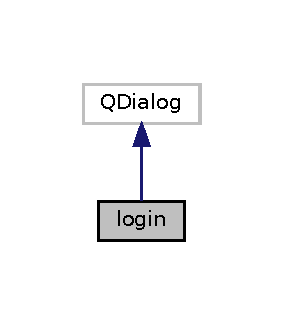
\includegraphics[width=136pt]{classlogin__inherit__graph}
\end{center}
\end{figure}


Collaboration diagram for login\+:
\nopagebreak
\begin{figure}[H]
\begin{center}
\leavevmode
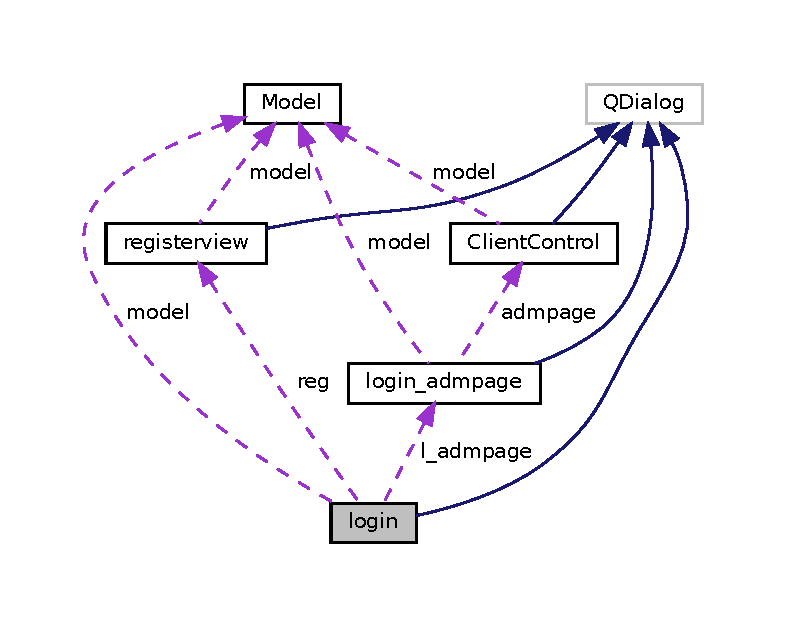
\includegraphics[width=350pt]{classlogin__coll__graph}
\end{center}
\end{figure}
\subsection*{Public Member Functions}
\begin{DoxyCompactItemize}
\item 
\hyperlink{classlogin_ab0ef02ae84a8c877a3da00c9bb600d44}{login} (Q\+Widget $\ast$parent=nullptr)
\begin{DoxyCompactList}\small\item\em Construct a new Login object. \end{DoxyCompactList}\item 
\hyperlink{classlogin_a4086fe44ad1e40447a0bebbc9b8b3c14}{$\sim$login} ()
\begin{DoxyCompactList}\small\item\em Destroy the Login object. \end{DoxyCompactList}\item 
\hyperlink{classregisterview}{registerview} $\ast$ \hyperlink{classlogin_a4a6b52d07ff54425b77eeb2625c413e7}{get\+Reg} () const
\begin{DoxyCompactList}\small\item\em Get the Reg object. \end{DoxyCompactList}\item 
void \hyperlink{classlogin_a139cc269e6d71c7f2650acff4cf1cd77}{set\+Reg} (\hyperlink{classregisterview}{registerview} $\ast$value)
\begin{DoxyCompactList}\small\item\em Set the Reg object. \end{DoxyCompactList}\item 
\hyperlink{classModel}{Model} $\ast$ \hyperlink{classlogin_a39618a46d937fed5e8d29c652a08ba8d}{get\+Model} () const
\begin{DoxyCompactList}\small\item\em Get the \hyperlink{classModel}{Model} object. \end{DoxyCompactList}\item 
void \hyperlink{classlogin_ae5f30c876e40c092ff18b88ea740d528}{set\+Model} (\hyperlink{classModel}{Model} $\ast$value)
\begin{DoxyCompactList}\small\item\em Set the \hyperlink{classModel}{Model} object. \end{DoxyCompactList}\item 
\hyperlink{classlogin__admpage}{login\+\_\+admpage} $\ast$ \hyperlink{classlogin_a4be030346534b2d066c33c0a28f2eb68}{get\+Login\+Adm\+Page} () const
\begin{DoxyCompactList}\small\item\em Get the Login Adm Page object. \end{DoxyCompactList}\item 
void \hyperlink{classlogin_a30d139e6c1e4eeea8c23776e23cc8e47}{set\+Login\+Adm\+Page} (\hyperlink{classlogin__admpage}{login\+\_\+admpage} $\ast$value)
\begin{DoxyCompactList}\small\item\em Set the Login Adm Page object. \end{DoxyCompactList}\end{DoxyCompactItemize}
\subsection*{Private Slots}
\begin{DoxyCompactItemize}
\item 
void \hyperlink{classlogin_afd45d9eb7e10b36d5b40f598de3fa2c8}{on\+\_\+btn\+\_\+adm\+Page\+\_\+clicked} ()
\begin{DoxyCompactList}\small\item\em the function button to redirect to the Admpage \end{DoxyCompactList}\item 
void \hyperlink{classlogin_a443d3a41176756820926a515cbd4cd1f}{on\+\_\+push\+Button\+\_\+clicked} ()
\begin{DoxyCompactList}\small\item\em the function button \end{DoxyCompactList}\item 
void \hyperlink{classlogin_aad5cd482a25f3c951bd5ecf1d12bb1a5}{on\+\_\+btn\+\_\+new\+Client\+\_\+clicked} ()
\begin{DoxyCompactList}\small\item\em the function button to redirect to the register user view \end{DoxyCompactList}\end{DoxyCompactItemize}
\subsection*{Private Attributes}
\begin{DoxyCompactItemize}
\item 
Ui\+::login $\ast$ \hyperlink{classlogin_ab08986017bf8d41e5cbab46dd0492d38}{ui}
\item 
\hyperlink{classModel}{Model} $\ast$ \hyperlink{classlogin_a2e047dc21e76732165598efabd633aa4}{model}
\item 
\hyperlink{classregisterview}{registerview} $\ast$ \hyperlink{classlogin_ae69e30e8855dbf4a08d3080edc6fcde4}{reg}
\item 
\hyperlink{classlogin__admpage}{login\+\_\+admpage} $\ast$ \hyperlink{classlogin_ac0ba28b943ddc71777895e7144ac26a6}{l\+\_\+admpage}
\end{DoxyCompactItemize}


\subsection{Detailed Description}
this class representer a Login UI 

\subsection{Constructor \& Destructor Documentation}
\mbox{\Hypertarget{classlogin_ab0ef02ae84a8c877a3da00c9bb600d44}\label{classlogin_ab0ef02ae84a8c877a3da00c9bb600d44}} 
\index{login@{login}!login@{login}}
\index{login@{login}!login@{login}}
\subsubsection{\texorpdfstring{login()}{login()}}
{\footnotesize\ttfamily login\+::login (\begin{DoxyParamCaption}\item[{Q\+Widget $\ast$}]{parent = {\ttfamily nullptr} }\end{DoxyParamCaption})\hspace{0.3cm}{\ttfamily [explicit]}}



Construct a new Login object. 


\begin{DoxyParams}{Parameters}
{\em parent} & \\
\hline
\end{DoxyParams}
\mbox{\Hypertarget{classlogin_a4086fe44ad1e40447a0bebbc9b8b3c14}\label{classlogin_a4086fe44ad1e40447a0bebbc9b8b3c14}} 
\index{login@{login}!````~login@{$\sim$login}}
\index{````~login@{$\sim$login}!login@{login}}
\subsubsection{\texorpdfstring{$\sim$login()}{~login()}}
{\footnotesize\ttfamily login\+::$\sim$login (\begin{DoxyParamCaption}{ }\end{DoxyParamCaption})}



Destroy the Login object. 



\subsection{Member Function Documentation}
\mbox{\Hypertarget{classlogin_a4be030346534b2d066c33c0a28f2eb68}\label{classlogin_a4be030346534b2d066c33c0a28f2eb68}} 
\index{login@{login}!get\+Login\+Adm\+Page@{get\+Login\+Adm\+Page}}
\index{get\+Login\+Adm\+Page@{get\+Login\+Adm\+Page}!login@{login}}
\subsubsection{\texorpdfstring{get\+Login\+Adm\+Page()}{getLoginAdmPage()}}
{\footnotesize\ttfamily \hyperlink{classlogin__admpage}{login\+\_\+admpage} $\ast$ login\+::get\+Login\+Adm\+Page (\begin{DoxyParamCaption}{ }\end{DoxyParamCaption}) const}



Get the Login Adm Page object. 

\begin{DoxyReturn}{Returns}
login\+\_\+admpage$\ast$ the Login\textquotesingle{}s Admpage 
\end{DoxyReturn}
\mbox{\Hypertarget{classlogin_a39618a46d937fed5e8d29c652a08ba8d}\label{classlogin_a39618a46d937fed5e8d29c652a08ba8d}} 
\index{login@{login}!get\+Model@{get\+Model}}
\index{get\+Model@{get\+Model}!login@{login}}
\subsubsection{\texorpdfstring{get\+Model()}{getModel()}}
{\footnotesize\ttfamily \hyperlink{classModel}{Model} $\ast$ login\+::get\+Model (\begin{DoxyParamCaption}{ }\end{DoxyParamCaption}) const}



Get the \hyperlink{classModel}{Model} object. 

\begin{DoxyReturn}{Returns}
Model$\ast$ the Login\textquotesingle{}s model 
\end{DoxyReturn}
\mbox{\Hypertarget{classlogin_a4a6b52d07ff54425b77eeb2625c413e7}\label{classlogin_a4a6b52d07ff54425b77eeb2625c413e7}} 
\index{login@{login}!get\+Reg@{get\+Reg}}
\index{get\+Reg@{get\+Reg}!login@{login}}
\subsubsection{\texorpdfstring{get\+Reg()}{getReg()}}
{\footnotesize\ttfamily \hyperlink{classregisterview}{registerview} $\ast$ login\+::get\+Reg (\begin{DoxyParamCaption}{ }\end{DoxyParamCaption}) const}



Get the Reg object. 

\begin{DoxyReturn}{Returns}
Register\+View$\ast$ the register\+View pointer 
\end{DoxyReturn}
\mbox{\Hypertarget{classlogin_afd45d9eb7e10b36d5b40f598de3fa2c8}\label{classlogin_afd45d9eb7e10b36d5b40f598de3fa2c8}} 
\index{login@{login}!on\+\_\+btn\+\_\+adm\+Page\+\_\+clicked@{on\+\_\+btn\+\_\+adm\+Page\+\_\+clicked}}
\index{on\+\_\+btn\+\_\+adm\+Page\+\_\+clicked@{on\+\_\+btn\+\_\+adm\+Page\+\_\+clicked}!login@{login}}
\subsubsection{\texorpdfstring{on\+\_\+btn\+\_\+adm\+Page\+\_\+clicked}{on\_btn\_admPage\_clicked}}
{\footnotesize\ttfamily void login\+::on\+\_\+btn\+\_\+adm\+Page\+\_\+clicked (\begin{DoxyParamCaption}{ }\end{DoxyParamCaption})\hspace{0.3cm}{\ttfamily [private]}, {\ttfamily [slot]}}



the function button to redirect to the Admpage 

\mbox{\Hypertarget{classlogin_aad5cd482a25f3c951bd5ecf1d12bb1a5}\label{classlogin_aad5cd482a25f3c951bd5ecf1d12bb1a5}} 
\index{login@{login}!on\+\_\+btn\+\_\+new\+Client\+\_\+clicked@{on\+\_\+btn\+\_\+new\+Client\+\_\+clicked}}
\index{on\+\_\+btn\+\_\+new\+Client\+\_\+clicked@{on\+\_\+btn\+\_\+new\+Client\+\_\+clicked}!login@{login}}
\subsubsection{\texorpdfstring{on\+\_\+btn\+\_\+new\+Client\+\_\+clicked}{on\_btn\_newClient\_clicked}}
{\footnotesize\ttfamily void login\+::on\+\_\+btn\+\_\+new\+Client\+\_\+clicked (\begin{DoxyParamCaption}{ }\end{DoxyParamCaption})\hspace{0.3cm}{\ttfamily [private]}, {\ttfamily [slot]}}



the function button to redirect to the register user view 

\mbox{\Hypertarget{classlogin_a443d3a41176756820926a515cbd4cd1f}\label{classlogin_a443d3a41176756820926a515cbd4cd1f}} 
\index{login@{login}!on\+\_\+push\+Button\+\_\+clicked@{on\+\_\+push\+Button\+\_\+clicked}}
\index{on\+\_\+push\+Button\+\_\+clicked@{on\+\_\+push\+Button\+\_\+clicked}!login@{login}}
\subsubsection{\texorpdfstring{on\+\_\+push\+Button\+\_\+clicked}{on\_pushButton\_clicked}}
{\footnotesize\ttfamily void login\+::on\+\_\+push\+Button\+\_\+clicked (\begin{DoxyParamCaption}{ }\end{DoxyParamCaption})\hspace{0.3cm}{\ttfamily [private]}, {\ttfamily [slot]}}



the function button 

\mbox{\Hypertarget{classlogin_a30d139e6c1e4eeea8c23776e23cc8e47}\label{classlogin_a30d139e6c1e4eeea8c23776e23cc8e47}} 
\index{login@{login}!set\+Login\+Adm\+Page@{set\+Login\+Adm\+Page}}
\index{set\+Login\+Adm\+Page@{set\+Login\+Adm\+Page}!login@{login}}
\subsubsection{\texorpdfstring{set\+Login\+Adm\+Page()}{setLoginAdmPage()}}
{\footnotesize\ttfamily void login\+::set\+Login\+Adm\+Page (\begin{DoxyParamCaption}\item[{\hyperlink{classlogin__admpage}{login\+\_\+admpage} $\ast$}]{value }\end{DoxyParamCaption})}



Set the Login Adm Page object. 


\begin{DoxyParams}{Parameters}
{\em value} & the new Login\textquotesingle{}s Admpage \\
\hline
\end{DoxyParams}
\mbox{\Hypertarget{classlogin_ae5f30c876e40c092ff18b88ea740d528}\label{classlogin_ae5f30c876e40c092ff18b88ea740d528}} 
\index{login@{login}!set\+Model@{set\+Model}}
\index{set\+Model@{set\+Model}!login@{login}}
\subsubsection{\texorpdfstring{set\+Model()}{setModel()}}
{\footnotesize\ttfamily void login\+::set\+Model (\begin{DoxyParamCaption}\item[{\hyperlink{classModel}{Model} $\ast$}]{value }\end{DoxyParamCaption})}



Set the \hyperlink{classModel}{Model} object. 


\begin{DoxyParams}{Parameters}
{\em value} & the Login\textquotesingle{}s new model \\
\hline
\end{DoxyParams}
\mbox{\Hypertarget{classlogin_a139cc269e6d71c7f2650acff4cf1cd77}\label{classlogin_a139cc269e6d71c7f2650acff4cf1cd77}} 
\index{login@{login}!set\+Reg@{set\+Reg}}
\index{set\+Reg@{set\+Reg}!login@{login}}
\subsubsection{\texorpdfstring{set\+Reg()}{setReg()}}
{\footnotesize\ttfamily void login\+::set\+Reg (\begin{DoxyParamCaption}\item[{\hyperlink{classregisterview}{registerview} $\ast$}]{value }\end{DoxyParamCaption})}



Set the Reg object. 


\begin{DoxyParams}{Parameters}
{\em value} & the register\+View pointer \\
\hline
\end{DoxyParams}


\subsection{Member Data Documentation}
\mbox{\Hypertarget{classlogin_ac0ba28b943ddc71777895e7144ac26a6}\label{classlogin_ac0ba28b943ddc71777895e7144ac26a6}} 
\index{login@{login}!l\+\_\+admpage@{l\+\_\+admpage}}
\index{l\+\_\+admpage@{l\+\_\+admpage}!login@{login}}
\subsubsection{\texorpdfstring{l\+\_\+admpage}{l\_admpage}}
{\footnotesize\ttfamily \hyperlink{classlogin__admpage}{login\+\_\+admpage}$\ast$ login\+::l\+\_\+admpage\hspace{0.3cm}{\ttfamily [private]}}

\mbox{\Hypertarget{classlogin_a2e047dc21e76732165598efabd633aa4}\label{classlogin_a2e047dc21e76732165598efabd633aa4}} 
\index{login@{login}!model@{model}}
\index{model@{model}!login@{login}}
\subsubsection{\texorpdfstring{model}{model}}
{\footnotesize\ttfamily \hyperlink{classModel}{Model}$\ast$ login\+::model\hspace{0.3cm}{\ttfamily [private]}}

\mbox{\Hypertarget{classlogin_ae69e30e8855dbf4a08d3080edc6fcde4}\label{classlogin_ae69e30e8855dbf4a08d3080edc6fcde4}} 
\index{login@{login}!reg@{reg}}
\index{reg@{reg}!login@{login}}
\subsubsection{\texorpdfstring{reg}{reg}}
{\footnotesize\ttfamily \hyperlink{classregisterview}{registerview}$\ast$ login\+::reg\hspace{0.3cm}{\ttfamily [private]}}

\mbox{\Hypertarget{classlogin_ab08986017bf8d41e5cbab46dd0492d38}\label{classlogin_ab08986017bf8d41e5cbab46dd0492d38}} 
\index{login@{login}!ui@{ui}}
\index{ui@{ui}!login@{login}}
\subsubsection{\texorpdfstring{ui}{ui}}
{\footnotesize\ttfamily Ui\+::login$\ast$ login\+::ui\hspace{0.3cm}{\ttfamily [private]}}



The documentation for this class was generated from the following files\+:\begin{DoxyCompactItemize}
\item 
views/\hyperlink{login_8h}{login.\+h}\item 
views/\hyperlink{login_8cpp}{login.\+cpp}\end{DoxyCompactItemize}

\hypertarget{classlogin__admpage}{}\section{login\+\_\+admpage Class Reference}
\label{classlogin__admpage}\index{login\+\_\+admpage@{login\+\_\+admpage}}


this class represents the authentication performed by the administrator before being redirected to the administrative page  




{\ttfamily \#include $<$login\+\_\+admpage.\+h$>$}



Inheritance diagram for login\+\_\+admpage\+:
\nopagebreak
\begin{figure}[H]
\begin{center}
\leavevmode
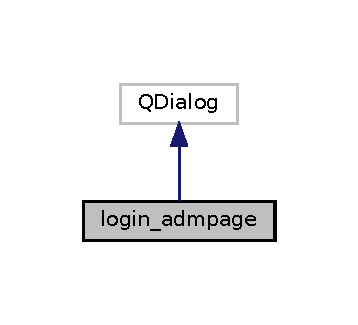
\includegraphics[width=172pt]{classlogin__admpage__inherit__graph}
\end{center}
\end{figure}


Collaboration diagram for login\+\_\+admpage\+:
\nopagebreak
\begin{figure}[H]
\begin{center}
\leavevmode
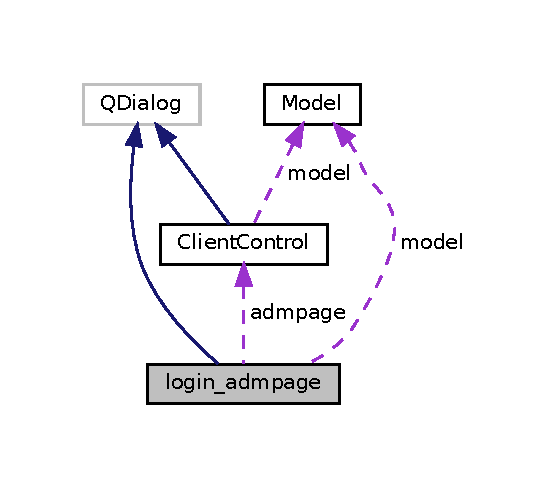
\includegraphics[width=263pt]{classlogin__admpage__coll__graph}
\end{center}
\end{figure}
\subsection*{Public Member Functions}
\begin{DoxyCompactItemize}
\item 
\hyperlink{classlogin__admpage_a36c9365b61928fc1be6387e87be814ba}{login\+\_\+admpage} (Q\+Widget $\ast$parent=nullptr)
\begin{DoxyCompactList}\small\item\em Construct a new login admpage object. \end{DoxyCompactList}\item 
\hyperlink{classlogin__admpage_a48e361ef6611dfa6e16810b53b7a9e13}{$\sim$login\+\_\+admpage} ()
\begin{DoxyCompactList}\small\item\em Destroy the login admpage object. \end{DoxyCompactList}\item 
\hyperlink{classModel}{Model} $\ast$ \hyperlink{classlogin__admpage_a6765491709543f3d887989ce9e76917d}{get\+Model} () const
\begin{DoxyCompactList}\small\item\em Get the \hyperlink{classModel}{Model} object. \end{DoxyCompactList}\item 
void \hyperlink{classlogin__admpage_a352ce22e69379a399169ce1f298a613e}{set\+Model} (\hyperlink{classModel}{Model} $\ast$value)
\begin{DoxyCompactList}\small\item\em Set the \hyperlink{classModel}{Model} object. \end{DoxyCompactList}\item 
\hyperlink{classClientControl}{Client\+Control} $\ast$ \hyperlink{classlogin__admpage_ab56e43d37e9f9944afbcb17f3740b365}{get\+Client\+Control} () const
\begin{DoxyCompactList}\small\item\em Get the Client Control object. \end{DoxyCompactList}\item 
void \hyperlink{classlogin__admpage_ae14083eb7d35e84e666b65124814a9f2}{set\+Client\+Control} (\hyperlink{classClientControl}{Client\+Control} $\ast$value)
\begin{DoxyCompactList}\small\item\em Set the Client Control object. \end{DoxyCompactList}\end{DoxyCompactItemize}
\subsection*{Private Slots}
\begin{DoxyCompactItemize}
\item 
void \hyperlink{classlogin__admpage_a5c5d7211f6efd8808e4af7ac4b935b25}{on\+\_\+push\+Button\+\_\+clicked} ()
\begin{DoxyCompactList}\small\item\em the button to validate the login \end{DoxyCompactList}\end{DoxyCompactItemize}
\subsection*{Private Attributes}
\begin{DoxyCompactItemize}
\item 
Ui\+::login\+\_\+admpage $\ast$ \hyperlink{classlogin__admpage_a2cffa7dd24ff7c387d80bfc8bc8e2e55}{ui}
\item 
\hyperlink{classModel}{Model} $\ast$ \hyperlink{classlogin__admpage_a6bef6e4a441d314925df6759abf81fd4}{model}
\item 
\hyperlink{classClientControl}{Client\+Control} $\ast$ \hyperlink{classlogin__admpage_aff7598c838503fc7bd8cf0754199e278}{admpage}
\end{DoxyCompactItemize}


\subsection{Detailed Description}
this class represents the authentication performed by the administrator before being redirected to the administrative page 

\subsection{Constructor \& Destructor Documentation}
\mbox{\Hypertarget{classlogin__admpage_a36c9365b61928fc1be6387e87be814ba}\label{classlogin__admpage_a36c9365b61928fc1be6387e87be814ba}} 
\index{login\+\_\+admpage@{login\+\_\+admpage}!login\+\_\+admpage@{login\+\_\+admpage}}
\index{login\+\_\+admpage@{login\+\_\+admpage}!login\+\_\+admpage@{login\+\_\+admpage}}
\subsubsection{\texorpdfstring{login\+\_\+admpage()}{login\_admpage()}}
{\footnotesize\ttfamily login\+\_\+admpage\+::login\+\_\+admpage (\begin{DoxyParamCaption}\item[{Q\+Widget $\ast$}]{parent = {\ttfamily nullptr} }\end{DoxyParamCaption})\hspace{0.3cm}{\ttfamily [explicit]}}



Construct a new login admpage object. 


\begin{DoxyParams}{Parameters}
{\em parent} & \\
\hline
\end{DoxyParams}
\mbox{\Hypertarget{classlogin__admpage_a48e361ef6611dfa6e16810b53b7a9e13}\label{classlogin__admpage_a48e361ef6611dfa6e16810b53b7a9e13}} 
\index{login\+\_\+admpage@{login\+\_\+admpage}!````~login\+\_\+admpage@{$\sim$login\+\_\+admpage}}
\index{````~login\+\_\+admpage@{$\sim$login\+\_\+admpage}!login\+\_\+admpage@{login\+\_\+admpage}}
\subsubsection{\texorpdfstring{$\sim$login\+\_\+admpage()}{~login\_admpage()}}
{\footnotesize\ttfamily login\+\_\+admpage\+::$\sim$login\+\_\+admpage (\begin{DoxyParamCaption}{ }\end{DoxyParamCaption})}



Destroy the login admpage object. 



\subsection{Member Function Documentation}
\mbox{\Hypertarget{classlogin__admpage_ab56e43d37e9f9944afbcb17f3740b365}\label{classlogin__admpage_ab56e43d37e9f9944afbcb17f3740b365}} 
\index{login\+\_\+admpage@{login\+\_\+admpage}!get\+Client\+Control@{get\+Client\+Control}}
\index{get\+Client\+Control@{get\+Client\+Control}!login\+\_\+admpage@{login\+\_\+admpage}}
\subsubsection{\texorpdfstring{get\+Client\+Control()}{getClientControl()}}
{\footnotesize\ttfamily \hyperlink{classClientControl}{Client\+Control} $\ast$ login\+\_\+admpage\+::get\+Client\+Control (\begin{DoxyParamCaption}{ }\end{DoxyParamCaption}) const}



Get the Client Control object. 

\begin{DoxyReturn}{Returns}
Client\+Control$\ast$ the Client Control page to be redirected 
\end{DoxyReturn}
\mbox{\Hypertarget{classlogin__admpage_a6765491709543f3d887989ce9e76917d}\label{classlogin__admpage_a6765491709543f3d887989ce9e76917d}} 
\index{login\+\_\+admpage@{login\+\_\+admpage}!get\+Model@{get\+Model}}
\index{get\+Model@{get\+Model}!login\+\_\+admpage@{login\+\_\+admpage}}
\subsubsection{\texorpdfstring{get\+Model()}{getModel()}}
{\footnotesize\ttfamily \hyperlink{classModel}{Model} $\ast$ login\+\_\+admpage\+::get\+Model (\begin{DoxyParamCaption}{ }\end{DoxyParamCaption}) const}



Get the \hyperlink{classModel}{Model} object. 

\begin{DoxyReturn}{Returns}
Model$\ast$ the Login\textquotesingle{}s model 
\end{DoxyReturn}
\mbox{\Hypertarget{classlogin__admpage_a5c5d7211f6efd8808e4af7ac4b935b25}\label{classlogin__admpage_a5c5d7211f6efd8808e4af7ac4b935b25}} 
\index{login\+\_\+admpage@{login\+\_\+admpage}!on\+\_\+push\+Button\+\_\+clicked@{on\+\_\+push\+Button\+\_\+clicked}}
\index{on\+\_\+push\+Button\+\_\+clicked@{on\+\_\+push\+Button\+\_\+clicked}!login\+\_\+admpage@{login\+\_\+admpage}}
\subsubsection{\texorpdfstring{on\+\_\+push\+Button\+\_\+clicked}{on\_pushButton\_clicked}}
{\footnotesize\ttfamily void login\+\_\+admpage\+::on\+\_\+push\+Button\+\_\+clicked (\begin{DoxyParamCaption}{ }\end{DoxyParamCaption})\hspace{0.3cm}{\ttfamily [private]}, {\ttfamily [slot]}}



the button to validate the login 

\mbox{\Hypertarget{classlogin__admpage_ae14083eb7d35e84e666b65124814a9f2}\label{classlogin__admpage_ae14083eb7d35e84e666b65124814a9f2}} 
\index{login\+\_\+admpage@{login\+\_\+admpage}!set\+Client\+Control@{set\+Client\+Control}}
\index{set\+Client\+Control@{set\+Client\+Control}!login\+\_\+admpage@{login\+\_\+admpage}}
\subsubsection{\texorpdfstring{set\+Client\+Control()}{setClientControl()}}
{\footnotesize\ttfamily void login\+\_\+admpage\+::set\+Client\+Control (\begin{DoxyParamCaption}\item[{\hyperlink{classClientControl}{Client\+Control} $\ast$}]{value }\end{DoxyParamCaption})}



Set the Client Control object. 


\begin{DoxyParams}{Parameters}
{\em value} & the new Client Control page \\
\hline
\end{DoxyParams}
\mbox{\Hypertarget{classlogin__admpage_a352ce22e69379a399169ce1f298a613e}\label{classlogin__admpage_a352ce22e69379a399169ce1f298a613e}} 
\index{login\+\_\+admpage@{login\+\_\+admpage}!set\+Model@{set\+Model}}
\index{set\+Model@{set\+Model}!login\+\_\+admpage@{login\+\_\+admpage}}
\subsubsection{\texorpdfstring{set\+Model()}{setModel()}}
{\footnotesize\ttfamily void login\+\_\+admpage\+::set\+Model (\begin{DoxyParamCaption}\item[{\hyperlink{classModel}{Model} $\ast$}]{value }\end{DoxyParamCaption})}



Set the \hyperlink{classModel}{Model} object. 


\begin{DoxyParams}{Parameters}
{\em value} & The new model \\
\hline
\end{DoxyParams}


\subsection{Member Data Documentation}
\mbox{\Hypertarget{classlogin__admpage_aff7598c838503fc7bd8cf0754199e278}\label{classlogin__admpage_aff7598c838503fc7bd8cf0754199e278}} 
\index{login\+\_\+admpage@{login\+\_\+admpage}!admpage@{admpage}}
\index{admpage@{admpage}!login\+\_\+admpage@{login\+\_\+admpage}}
\subsubsection{\texorpdfstring{admpage}{admpage}}
{\footnotesize\ttfamily \hyperlink{classClientControl}{Client\+Control}$\ast$ login\+\_\+admpage\+::admpage\hspace{0.3cm}{\ttfamily [private]}}

\mbox{\Hypertarget{classlogin__admpage_a6bef6e4a441d314925df6759abf81fd4}\label{classlogin__admpage_a6bef6e4a441d314925df6759abf81fd4}} 
\index{login\+\_\+admpage@{login\+\_\+admpage}!model@{model}}
\index{model@{model}!login\+\_\+admpage@{login\+\_\+admpage}}
\subsubsection{\texorpdfstring{model}{model}}
{\footnotesize\ttfamily \hyperlink{classModel}{Model}$\ast$ login\+\_\+admpage\+::model\hspace{0.3cm}{\ttfamily [private]}}

\mbox{\Hypertarget{classlogin__admpage_a2cffa7dd24ff7c387d80bfc8bc8e2e55}\label{classlogin__admpage_a2cffa7dd24ff7c387d80bfc8bc8e2e55}} 
\index{login\+\_\+admpage@{login\+\_\+admpage}!ui@{ui}}
\index{ui@{ui}!login\+\_\+admpage@{login\+\_\+admpage}}
\subsubsection{\texorpdfstring{ui}{ui}}
{\footnotesize\ttfamily Ui\+::login\+\_\+admpage$\ast$ login\+\_\+admpage\+::ui\hspace{0.3cm}{\ttfamily [private]}}



The documentation for this class was generated from the following files\+:\begin{DoxyCompactItemize}
\item 
views/\hyperlink{login__admpage_8h}{login\+\_\+admpage.\+h}\item 
views/\hyperlink{login__admpage_8cpp}{login\+\_\+admpage.\+cpp}\end{DoxyCompactItemize}

\hypertarget{classModel}{}\section{Model Class Reference}
\label{classModel}\index{Model@{Model}}


The \hyperlink{classModel}{Model} class.  




{\ttfamily \#include $<$model.\+h$>$}



Inheritance diagram for Model\+:\nopagebreak
\begin{figure}[H]
\begin{center}
\leavevmode
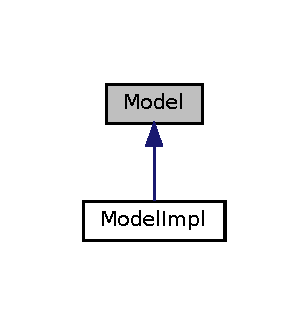
\includegraphics[width=148pt]{classModel__inherit__graph}
\end{center}
\end{figure}
\subsection*{Public Member Functions}
\begin{DoxyCompactItemize}
\item 
virtual \hyperlink{classModel_af032d8433c87a0a3a431faf6563a1f03}{$\sim$\+Model} ()
\begin{DoxyCompactList}\small\item\em Destroy the \hyperlink{classModel}{Model} object. \end{DoxyCompactList}\item 
virtual \hyperlink{classCourse}{Course} $\ast$ \hyperlink{classModel_ab62d035cd5240332e249d39ff9f98f9a}{create\+Course} (string, string, string)=0
\begin{DoxyCompactList}\small\item\em Create a \hyperlink{classCourse}{Course} object. \end{DoxyCompactList}\item 
virtual bool \hyperlink{classModel_acc20a58c9a9c7506b06df890e287433e}{remove\+Course} (\hyperlink{classCourse}{Course} $\ast$)=0
\begin{DoxyCompactList}\small\item\em Remove a \hyperlink{classCourse}{Course} object. \end{DoxyCompactList}\item 
virtual void \hyperlink{classModel_aa3ea9c92f586cec1944e3dcdee8c0672}{update\+Course} (\hyperlink{classCourse}{Course} $\ast$, string, string, string)=0
\begin{DoxyCompactList}\small\item\em Update a \hyperlink{classCourse}{Course} object. \end{DoxyCompactList}\item 
virtual vector$<$ \hyperlink{classCourse}{Course} $\ast$ $>$ \& \hyperlink{classModel_aded51911782e4fa19a79a423482dc561}{get\+Courses} ()=0
\begin{DoxyCompactList}\small\item\em Get the Courses object. \end{DoxyCompactList}\item 
virtual void \hyperlink{classModel_a9a4cc2b97cd97bc987f019dca7aa5d9e}{set\+Courses} (const vector$<$ \hyperlink{classCourse}{Course} $\ast$$>$ \&)=0
\begin{DoxyCompactList}\small\item\em Set the Courses object. \end{DoxyCompactList}\item 
virtual void \hyperlink{classModel_aff2385b433de34af14232ec8f7db126e}{add} (\hyperlink{classCourse}{Course} $\ast$)=0
\begin{DoxyCompactList}\small\item\em Adds a course to the model. \end{DoxyCompactList}\item 
virtual void \hyperlink{classModel_ab6bf3b0428a4b087e8126c4b203bfc45}{add\+User} (\hyperlink{classUser}{User} $\ast$)=0
\begin{DoxyCompactList}\small\item\em Adds a user to the model. \end{DoxyCompactList}\item 
virtual \hyperlink{classUser}{User} $\ast$ \hyperlink{classModel_a8080158d8cd5ff74bb0daae3824c220b}{create\+User} (string, string, string, string, const vector$<$ \hyperlink{classCourse}{Course} $\ast$$>$ \&, int)=0
\begin{DoxyCompactList}\small\item\em Create a \hyperlink{classUser}{User} object. \end{DoxyCompactList}\item 
virtual \hyperlink{classUser}{User} $\ast$ \hyperlink{classModel_a20cb9f90df3f8f235dc14fbc13b64167}{get\+User} () const =0
\begin{DoxyCompactList}\small\item\em Get the \hyperlink{classUser}{User} object. \end{DoxyCompactList}\item 
virtual void \hyperlink{classModel_aae120afc85d42a7bedee5405911986a5}{set\+User} (\hyperlink{classUser}{User} $\ast$)=0
\begin{DoxyCompactList}\small\item\em Set the \hyperlink{classUser}{User} object. \end{DoxyCompactList}\item 
virtual vector$<$ \hyperlink{classUser}{User} $\ast$ $>$ \& \hyperlink{classModel_a3e27c021561cb19ce48d4a456e75d5ab}{get\+User\+List} ()=0
\begin{DoxyCompactList}\small\item\em Get the \hyperlink{classUser}{User} List object. \end{DoxyCompactList}\item 
virtual void \hyperlink{classModel_affa0ad47e9417b52eca3b73105bad9f0}{set\+User\+List} (const vector$<$ \hyperlink{classUser}{User} $\ast$$>$ \&)=0
\begin{DoxyCompactList}\small\item\em Set the \hyperlink{classUser}{User} List object. \end{DoxyCompactList}\item 
virtual bool \hyperlink{classModel_ad217703837ecec908995225f6de1bfca}{remove\+User} (\hyperlink{classUser}{User} $\ast$)=0
\begin{DoxyCompactList}\small\item\em Remove a \hyperlink{classCourse}{Course} object. \end{DoxyCompactList}\item 
virtual void \hyperlink{classModel_a83ebd4a5678c31c8dd46155d34df961d}{update\+User} (\hyperlink{classUser}{User} $\ast$, string, string, string, string)=0
\begin{DoxyCompactList}\small\item\em Update a \hyperlink{classCourse}{Course} object. \end{DoxyCompactList}\item 
virtual bool \hyperlink{classModel_a4e75d78a6dc3ded41a44475c3d59aa57}{write\+Course} (const string \&)=0
\item 
virtual bool \hyperlink{classModel_a6a0784fa1dd4bffcebda8eb3bf38059e}{read\+Course} (const string \&)=0
\item 
virtual bool \hyperlink{classModel_ad2d1b50c1c071ad0b7820cf4343b2463}{write\+User} (const string \&)=0
\begin{DoxyCompactList}\small\item\em Write a file. \end{DoxyCompactList}\item 
virtual bool \hyperlink{classModel_ad3fa273a7dc1397ce748c657e552d6cc}{read\+User} (const string \&)=0
\begin{DoxyCompactList}\small\item\em Read a file. \end{DoxyCompactList}\end{DoxyCompactItemize}
\subsection*{Static Public Member Functions}
\begin{DoxyCompactItemize}
\item 
static \hyperlink{classModel}{Model} $\ast$ \hyperlink{classModel_accd28300871325fce68d551cebf27220}{create\+Model} ()
\begin{DoxyCompactList}\small\item\em Create a \hyperlink{classModel}{Model} object. \end{DoxyCompactList}\end{DoxyCompactItemize}


\subsection{Detailed Description}
The \hyperlink{classModel}{Model} class. 

\subsection{Constructor \& Destructor Documentation}
\mbox{\Hypertarget{classModel_af032d8433c87a0a3a431faf6563a1f03}\label{classModel_af032d8433c87a0a3a431faf6563a1f03}} 
\index{Model@{Model}!````~Model@{$\sim$\+Model}}
\index{````~Model@{$\sim$\+Model}!Model@{Model}}
\subsubsection{\texorpdfstring{$\sim$\+Model()}{~Model()}}
{\footnotesize\ttfamily virtual Model\+::$\sim$\+Model (\begin{DoxyParamCaption}{ }\end{DoxyParamCaption})\hspace{0.3cm}{\ttfamily [inline]}, {\ttfamily [virtual]}}



Destroy the \hyperlink{classModel}{Model} object. 



\subsection{Member Function Documentation}
\mbox{\Hypertarget{classModel_aff2385b433de34af14232ec8f7db126e}\label{classModel_aff2385b433de34af14232ec8f7db126e}} 
\index{Model@{Model}!add@{add}}
\index{add@{add}!Model@{Model}}
\subsubsection{\texorpdfstring{add()}{add()}}
{\footnotesize\ttfamily virtual void Model\+::add (\begin{DoxyParamCaption}\item[{\hyperlink{classCourse}{Course} $\ast$}]{ }\end{DoxyParamCaption})\hspace{0.3cm}{\ttfamily [pure virtual]}}



Adds a course to the model. 



Implemented in \hyperlink{classModelImpl_a1847f819acc9bf909e31ec3438973225}{Model\+Impl}.

\mbox{\Hypertarget{classModel_ab6bf3b0428a4b087e8126c4b203bfc45}\label{classModel_ab6bf3b0428a4b087e8126c4b203bfc45}} 
\index{Model@{Model}!add\+User@{add\+User}}
\index{add\+User@{add\+User}!Model@{Model}}
\subsubsection{\texorpdfstring{add\+User()}{addUser()}}
{\footnotesize\ttfamily virtual void Model\+::add\+User (\begin{DoxyParamCaption}\item[{\hyperlink{classUser}{User} $\ast$}]{ }\end{DoxyParamCaption})\hspace{0.3cm}{\ttfamily [pure virtual]}}



Adds a user to the model. 



Implemented in \hyperlink{classModelImpl_aa0c7acd29ab42d13227e0e85fea044c8}{Model\+Impl}.

\mbox{\Hypertarget{classModel_ab62d035cd5240332e249d39ff9f98f9a}\label{classModel_ab62d035cd5240332e249d39ff9f98f9a}} 
\index{Model@{Model}!create\+Course@{create\+Course}}
\index{create\+Course@{create\+Course}!Model@{Model}}
\subsubsection{\texorpdfstring{create\+Course()}{createCourse()}}
{\footnotesize\ttfamily virtual \hyperlink{classCourse}{Course}$\ast$ Model\+::create\+Course (\begin{DoxyParamCaption}\item[{string}]{,  }\item[{string}]{,  }\item[{string}]{ }\end{DoxyParamCaption})\hspace{0.3cm}{\ttfamily [pure virtual]}}



Create a \hyperlink{classCourse}{Course} object. 

\begin{DoxyReturn}{Returns}
Course$\ast$ \hyperlink{classCourse}{Course} set. 
\end{DoxyReturn}


Implemented in \hyperlink{classModelImpl_a9bcdb7f3c69ac4f86f253a9422ae6ce9}{Model\+Impl}.

\mbox{\Hypertarget{classModel_accd28300871325fce68d551cebf27220}\label{classModel_accd28300871325fce68d551cebf27220}} 
\index{Model@{Model}!create\+Model@{create\+Model}}
\index{create\+Model@{create\+Model}!Model@{Model}}
\subsubsection{\texorpdfstring{create\+Model()}{createModel()}}
{\footnotesize\ttfamily \hyperlink{classModel}{Model} $\ast$ Model\+::create\+Model (\begin{DoxyParamCaption}{ }\end{DoxyParamCaption})\hspace{0.3cm}{\ttfamily [static]}}



Create a \hyperlink{classModel}{Model} object. 

\begin{DoxyReturn}{Returns}
Model$\ast$ \hyperlink{classModel}{Model} set. 
\end{DoxyReturn}
\mbox{\Hypertarget{classModel_a8080158d8cd5ff74bb0daae3824c220b}\label{classModel_a8080158d8cd5ff74bb0daae3824c220b}} 
\index{Model@{Model}!create\+User@{create\+User}}
\index{create\+User@{create\+User}!Model@{Model}}
\subsubsection{\texorpdfstring{create\+User()}{createUser()}}
{\footnotesize\ttfamily virtual \hyperlink{classUser}{User}$\ast$ Model\+::create\+User (\begin{DoxyParamCaption}\item[{string}]{,  }\item[{string}]{,  }\item[{string}]{,  }\item[{string}]{,  }\item[{const vector$<$ \hyperlink{classCourse}{Course} $\ast$$>$ \&}]{,  }\item[{int}]{ }\end{DoxyParamCaption})\hspace{0.3cm}{\ttfamily [pure virtual]}}



Create a \hyperlink{classUser}{User} object. 

\begin{DoxyReturn}{Returns}
User$\ast$ \hyperlink{classUser}{User} set 
\end{DoxyReturn}


Implemented in \hyperlink{classModelImpl_affad955ee2bdbfc58ac049632cd9668b}{Model\+Impl}.

\mbox{\Hypertarget{classModel_aded51911782e4fa19a79a423482dc561}\label{classModel_aded51911782e4fa19a79a423482dc561}} 
\index{Model@{Model}!get\+Courses@{get\+Courses}}
\index{get\+Courses@{get\+Courses}!Model@{Model}}
\subsubsection{\texorpdfstring{get\+Courses()}{getCourses()}}
{\footnotesize\ttfamily virtual vector$<$\hyperlink{classCourse}{Course}$\ast$$>$\& Model\+::get\+Courses (\begin{DoxyParamCaption}{ }\end{DoxyParamCaption})\hspace{0.3cm}{\ttfamily [pure virtual]}}



Get the Courses object. 

\begin{DoxyReturn}{Returns}
vector$<$\+Course$\ast$$>$\& Courses set 
\end{DoxyReturn}


Implemented in \hyperlink{classModelImpl_afc84ed40271afee13778f4e9f9f90e2e}{Model\+Impl}.

\mbox{\Hypertarget{classModel_a20cb9f90df3f8f235dc14fbc13b64167}\label{classModel_a20cb9f90df3f8f235dc14fbc13b64167}} 
\index{Model@{Model}!get\+User@{get\+User}}
\index{get\+User@{get\+User}!Model@{Model}}
\subsubsection{\texorpdfstring{get\+User()}{getUser()}}
{\footnotesize\ttfamily virtual \hyperlink{classUser}{User}$\ast$ Model\+::get\+User (\begin{DoxyParamCaption}{ }\end{DoxyParamCaption}) const\hspace{0.3cm}{\ttfamily [pure virtual]}}



Get the \hyperlink{classUser}{User} object. 

\begin{DoxyReturn}{Returns}
User$\ast$ \hyperlink{classUser}{User} set 
\end{DoxyReturn}


Implemented in \hyperlink{classModelImpl_ac098ad97916ff988d518ded5056dabb0}{Model\+Impl}.

\mbox{\Hypertarget{classModel_a3e27c021561cb19ce48d4a456e75d5ab}\label{classModel_a3e27c021561cb19ce48d4a456e75d5ab}} 
\index{Model@{Model}!get\+User\+List@{get\+User\+List}}
\index{get\+User\+List@{get\+User\+List}!Model@{Model}}
\subsubsection{\texorpdfstring{get\+User\+List()}{getUserList()}}
{\footnotesize\ttfamily virtual vector$<$\hyperlink{classUser}{User}$\ast$$>$\& Model\+::get\+User\+List (\begin{DoxyParamCaption}{ }\end{DoxyParamCaption})\hspace{0.3cm}{\ttfamily [pure virtual]}}



Get the \hyperlink{classUser}{User} List object. 

\begin{DoxyReturn}{Returns}
vector$<$\+User$\ast$$>$\& Users set 
\end{DoxyReturn}


Implemented in \hyperlink{classModelImpl_a46f441c1ba57cc395e6732cab80e78fd}{Model\+Impl}.

\mbox{\Hypertarget{classModel_a6a0784fa1dd4bffcebda8eb3bf38059e}\label{classModel_a6a0784fa1dd4bffcebda8eb3bf38059e}} 
\index{Model@{Model}!read\+Course@{read\+Course}}
\index{read\+Course@{read\+Course}!Model@{Model}}
\subsubsection{\texorpdfstring{read\+Course()}{readCourse()}}
{\footnotesize\ttfamily virtual bool Model\+::read\+Course (\begin{DoxyParamCaption}\item[{const string \&}]{ }\end{DoxyParamCaption})\hspace{0.3cm}{\ttfamily [pure virtual]}}



Implemented in \hyperlink{classModelImpl_aba86d399703fe35c086d6ff5647e48da}{Model\+Impl}.

\mbox{\Hypertarget{classModel_ad3fa273a7dc1397ce748c657e552d6cc}\label{classModel_ad3fa273a7dc1397ce748c657e552d6cc}} 
\index{Model@{Model}!read\+User@{read\+User}}
\index{read\+User@{read\+User}!Model@{Model}}
\subsubsection{\texorpdfstring{read\+User()}{readUser()}}
{\footnotesize\ttfamily virtual bool Model\+::read\+User (\begin{DoxyParamCaption}\item[{const string \&}]{ }\end{DoxyParamCaption})\hspace{0.3cm}{\ttfamily [pure virtual]}}



Read a file. 

\begin{DoxyReturn}{Returns}
true if it was successful 

false if it failed 
\end{DoxyReturn}


Implemented in \hyperlink{classModelImpl_a132c46a2d6ca86c7374a065b3079fe15}{Model\+Impl}.

\mbox{\Hypertarget{classModel_acc20a58c9a9c7506b06df890e287433e}\label{classModel_acc20a58c9a9c7506b06df890e287433e}} 
\index{Model@{Model}!remove\+Course@{remove\+Course}}
\index{remove\+Course@{remove\+Course}!Model@{Model}}
\subsubsection{\texorpdfstring{remove\+Course()}{removeCourse()}}
{\footnotesize\ttfamily virtual bool Model\+::remove\+Course (\begin{DoxyParamCaption}\item[{\hyperlink{classCourse}{Course} $\ast$}]{ }\end{DoxyParamCaption})\hspace{0.3cm}{\ttfamily [pure virtual]}}



Remove a \hyperlink{classCourse}{Course} object. 

\begin{DoxyReturn}{Returns}
true if it was successful 

false if it failed 
\end{DoxyReturn}


Implemented in \hyperlink{classModelImpl_ae46076a7e4b54d24ba15fb2eb8e7f33d}{Model\+Impl}.

\mbox{\Hypertarget{classModel_ad217703837ecec908995225f6de1bfca}\label{classModel_ad217703837ecec908995225f6de1bfca}} 
\index{Model@{Model}!remove\+User@{remove\+User}}
\index{remove\+User@{remove\+User}!Model@{Model}}
\subsubsection{\texorpdfstring{remove\+User()}{removeUser()}}
{\footnotesize\ttfamily virtual bool Model\+::remove\+User (\begin{DoxyParamCaption}\item[{\hyperlink{classUser}{User} $\ast$}]{ }\end{DoxyParamCaption})\hspace{0.3cm}{\ttfamily [pure virtual]}}



Remove a \hyperlink{classCourse}{Course} object. 

\begin{DoxyReturn}{Returns}
true if it was successful 

false if it failed 
\end{DoxyReturn}


Implemented in \hyperlink{classModelImpl_a51130aa538cd27b1cac6919cbbef05ee}{Model\+Impl}.

\mbox{\Hypertarget{classModel_a9a4cc2b97cd97bc987f019dca7aa5d9e}\label{classModel_a9a4cc2b97cd97bc987f019dca7aa5d9e}} 
\index{Model@{Model}!set\+Courses@{set\+Courses}}
\index{set\+Courses@{set\+Courses}!Model@{Model}}
\subsubsection{\texorpdfstring{set\+Courses()}{setCourses()}}
{\footnotesize\ttfamily virtual void Model\+::set\+Courses (\begin{DoxyParamCaption}\item[{const vector$<$ \hyperlink{classCourse}{Course} $\ast$$>$ \&}]{ }\end{DoxyParamCaption})\hspace{0.3cm}{\ttfamily [pure virtual]}}



Set the Courses object. 



Implemented in \hyperlink{classModelImpl_ae90d5e4e7ec786f3752a6551dab39d66}{Model\+Impl}.

\mbox{\Hypertarget{classModel_aae120afc85d42a7bedee5405911986a5}\label{classModel_aae120afc85d42a7bedee5405911986a5}} 
\index{Model@{Model}!set\+User@{set\+User}}
\index{set\+User@{set\+User}!Model@{Model}}
\subsubsection{\texorpdfstring{set\+User()}{setUser()}}
{\footnotesize\ttfamily virtual void Model\+::set\+User (\begin{DoxyParamCaption}\item[{\hyperlink{classUser}{User} $\ast$}]{ }\end{DoxyParamCaption})\hspace{0.3cm}{\ttfamily [pure virtual]}}



Set the \hyperlink{classUser}{User} object. 



Implemented in \hyperlink{classModelImpl_a9e1a1953a4d3355e147515c2a0b3c031}{Model\+Impl}.

\mbox{\Hypertarget{classModel_affa0ad47e9417b52eca3b73105bad9f0}\label{classModel_affa0ad47e9417b52eca3b73105bad9f0}} 
\index{Model@{Model}!set\+User\+List@{set\+User\+List}}
\index{set\+User\+List@{set\+User\+List}!Model@{Model}}
\subsubsection{\texorpdfstring{set\+User\+List()}{setUserList()}}
{\footnotesize\ttfamily virtual void Model\+::set\+User\+List (\begin{DoxyParamCaption}\item[{const vector$<$ \hyperlink{classUser}{User} $\ast$$>$ \&}]{ }\end{DoxyParamCaption})\hspace{0.3cm}{\ttfamily [pure virtual]}}



Set the \hyperlink{classUser}{User} List object. 



Implemented in \hyperlink{classModelImpl_a617c58790e2b2207a3ce7e860a56e3a1}{Model\+Impl}.

\mbox{\Hypertarget{classModel_aa3ea9c92f586cec1944e3dcdee8c0672}\label{classModel_aa3ea9c92f586cec1944e3dcdee8c0672}} 
\index{Model@{Model}!update\+Course@{update\+Course}}
\index{update\+Course@{update\+Course}!Model@{Model}}
\subsubsection{\texorpdfstring{update\+Course()}{updateCourse()}}
{\footnotesize\ttfamily virtual void Model\+::update\+Course (\begin{DoxyParamCaption}\item[{\hyperlink{classCourse}{Course} $\ast$}]{,  }\item[{string}]{,  }\item[{string}]{,  }\item[{string}]{ }\end{DoxyParamCaption})\hspace{0.3cm}{\ttfamily [pure virtual]}}



Update a \hyperlink{classCourse}{Course} object. 



Implemented in \hyperlink{classModelImpl_aec25920972acddf92114b2b3581b9d66}{Model\+Impl}.

\mbox{\Hypertarget{classModel_a83ebd4a5678c31c8dd46155d34df961d}\label{classModel_a83ebd4a5678c31c8dd46155d34df961d}} 
\index{Model@{Model}!update\+User@{update\+User}}
\index{update\+User@{update\+User}!Model@{Model}}
\subsubsection{\texorpdfstring{update\+User()}{updateUser()}}
{\footnotesize\ttfamily virtual void Model\+::update\+User (\begin{DoxyParamCaption}\item[{\hyperlink{classUser}{User} $\ast$}]{,  }\item[{string}]{,  }\item[{string}]{,  }\item[{string}]{,  }\item[{string}]{ }\end{DoxyParamCaption})\hspace{0.3cm}{\ttfamily [pure virtual]}}



Update a \hyperlink{classCourse}{Course} object. 



Implemented in \hyperlink{classModelImpl_a8088106fd8837da688f9334ab143db4c}{Model\+Impl}.

\mbox{\Hypertarget{classModel_a4e75d78a6dc3ded41a44475c3d59aa57}\label{classModel_a4e75d78a6dc3ded41a44475c3d59aa57}} 
\index{Model@{Model}!write\+Course@{write\+Course}}
\index{write\+Course@{write\+Course}!Model@{Model}}
\subsubsection{\texorpdfstring{write\+Course()}{writeCourse()}}
{\footnotesize\ttfamily virtual bool Model\+::write\+Course (\begin{DoxyParamCaption}\item[{const string \&}]{ }\end{DoxyParamCaption})\hspace{0.3cm}{\ttfamily [pure virtual]}}



Implemented in \hyperlink{classModelImpl_a6ce3d79c0b49abe19c034dfb30d023d7}{Model\+Impl}.

\mbox{\Hypertarget{classModel_ad2d1b50c1c071ad0b7820cf4343b2463}\label{classModel_ad2d1b50c1c071ad0b7820cf4343b2463}} 
\index{Model@{Model}!write\+User@{write\+User}}
\index{write\+User@{write\+User}!Model@{Model}}
\subsubsection{\texorpdfstring{write\+User()}{writeUser()}}
{\footnotesize\ttfamily virtual bool Model\+::write\+User (\begin{DoxyParamCaption}\item[{const string \&}]{ }\end{DoxyParamCaption})\hspace{0.3cm}{\ttfamily [pure virtual]}}



Write a file. 

\begin{DoxyReturn}{Returns}
true if it was successful 

false if it failed 
\end{DoxyReturn}


Implemented in \hyperlink{classModelImpl_a42b5948a513af3e20645cdb63fb6be76}{Model\+Impl}.



The documentation for this class was generated from the following files\+:\begin{DoxyCompactItemize}
\item 
src/lib/\hyperlink{model_8h}{model.\+h}\item 
src/lib/\hyperlink{model__impl_8cpp}{model\+\_\+impl.\+cpp}\end{DoxyCompactItemize}

\hypertarget{classModelImpl}{}\section{Model\+Impl Class Reference}
\label{classModelImpl}\index{Model\+Impl@{Model\+Impl}}


Derived class where all methods will be implemented according to the desired modeling.  




{\ttfamily \#include $<$model\+\_\+impl.\+h$>$}



Inheritance diagram for Model\+Impl\+:\nopagebreak
\begin{figure}[H]
\begin{center}
\leavevmode
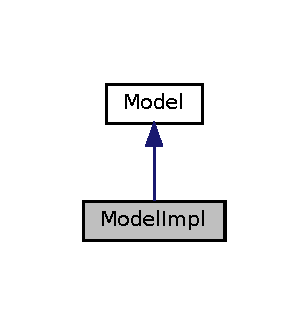
\includegraphics[width=148pt]{classModelImpl__inherit__graph}
\end{center}
\end{figure}


Collaboration diagram for Model\+Impl\+:\nopagebreak
\begin{figure}[H]
\begin{center}
\leavevmode
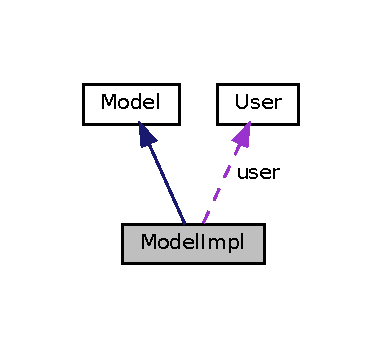
\includegraphics[width=184pt]{classModelImpl__coll__graph}
\end{center}
\end{figure}
\subsection*{Public Member Functions}
\begin{DoxyCompactItemize}
\item 
\hyperlink{classModelImpl_a081505846c37ce9928f2176d77db4bc8}{Model\+Impl} ()
\begin{DoxyCompactList}\small\item\em Construct a new \hyperlink{classModel}{Model} Impl object. \end{DoxyCompactList}\item 
\hyperlink{classModelImpl_a427f422a6d356b94afbe3937d6452a2b}{$\sim$\+Model\+Impl} ()
\begin{DoxyCompactList}\small\item\em Destroy the \hyperlink{classModel}{Model} Impl object. \end{DoxyCompactList}\item 
\hyperlink{classCourse}{Course} $\ast$ \hyperlink{classModelImpl_a9bcdb7f3c69ac4f86f253a9422ae6ce9}{create\+Course} (string, string, string)
\begin{DoxyCompactList}\small\item\em Create a \hyperlink{classCourse}{Course} object. \end{DoxyCompactList}\item 
bool \hyperlink{classModelImpl_ae46076a7e4b54d24ba15fb2eb8e7f33d}{remove\+Course} (\hyperlink{classCourse}{Course} $\ast$)
\begin{DoxyCompactList}\small\item\em Remove a \hyperlink{classCourse}{Course} object. \end{DoxyCompactList}\item 
void \hyperlink{classModelImpl_aec25920972acddf92114b2b3581b9d66}{update\+Course} (\hyperlink{classCourse}{Course} $\ast$, string, string, string)
\begin{DoxyCompactList}\small\item\em Update a \hyperlink{classCourse}{Course} object. \end{DoxyCompactList}\item 
vector$<$ \hyperlink{classCourse}{Course} $\ast$ $>$ \& \hyperlink{classModelImpl_afc84ed40271afee13778f4e9f9f90e2e}{get\+Courses} ()
\begin{DoxyCompactList}\small\item\em Get the Courses object. \end{DoxyCompactList}\item 
void \hyperlink{classModelImpl_ae90d5e4e7ec786f3752a6551dab39d66}{set\+Courses} (const vector$<$ \hyperlink{classCourse}{Course} $\ast$$>$ \&)
\begin{DoxyCompactList}\small\item\em Set the Courses object. \end{DoxyCompactList}\item 
void \hyperlink{classModelImpl_a1847f819acc9bf909e31ec3438973225}{add} (\hyperlink{classCourse}{Course} $\ast$)
\begin{DoxyCompactList}\small\item\em Adds a course to the model. \end{DoxyCompactList}\item 
void \hyperlink{classModelImpl_aa0c7acd29ab42d13227e0e85fea044c8}{add\+User} (\hyperlink{classUser}{User} $\ast$\hyperlink{classModelImpl_a76f8d6f7634f9395c2576a5d11628e13}{user})
\begin{DoxyCompactList}\small\item\em Adds a user to the model. \end{DoxyCompactList}\item 
\hyperlink{classUser}{User} $\ast$ \hyperlink{classModelImpl_affad955ee2bdbfc58ac049632cd9668b}{create\+User} (string, string, string, string, const vector$<$ \hyperlink{classCourse}{Course} $\ast$$>$ \&, int)
\begin{DoxyCompactList}\small\item\em Create a \hyperlink{classUser}{User} object. \end{DoxyCompactList}\item 
\hyperlink{classUser}{User} $\ast$ \hyperlink{classModelImpl_ac098ad97916ff988d518ded5056dabb0}{get\+User} () const
\begin{DoxyCompactList}\small\item\em Get the \hyperlink{classUser}{User} object. \end{DoxyCompactList}\item 
void \hyperlink{classModelImpl_a9e1a1953a4d3355e147515c2a0b3c031}{set\+User} (\hyperlink{classUser}{User} $\ast$)
\begin{DoxyCompactList}\small\item\em Set the \hyperlink{classUser}{User} object. \end{DoxyCompactList}\item 
vector$<$ \hyperlink{classUser}{User} $\ast$ $>$ \& \hyperlink{classModelImpl_a46f441c1ba57cc395e6732cab80e78fd}{get\+User\+List} ()
\begin{DoxyCompactList}\small\item\em Get the \hyperlink{classUser}{User} List object. \end{DoxyCompactList}\item 
void \hyperlink{classModelImpl_a617c58790e2b2207a3ce7e860a56e3a1}{set\+User\+List} (const vector$<$ \hyperlink{classUser}{User} $\ast$$>$ \&)
\begin{DoxyCompactList}\small\item\em Set the \hyperlink{classUser}{User} List object. \end{DoxyCompactList}\item 
bool \hyperlink{classModelImpl_a51130aa538cd27b1cac6919cbbef05ee}{remove\+User} (\hyperlink{classUser}{User} $\ast$)
\begin{DoxyCompactList}\small\item\em Remove a \hyperlink{classCourse}{Course} object. \end{DoxyCompactList}\item 
void \hyperlink{classModelImpl_a8088106fd8837da688f9334ab143db4c}{update\+User} (\hyperlink{classUser}{User} $\ast$, string, string, string, string)
\begin{DoxyCompactList}\small\item\em Update a \hyperlink{classCourse}{Course} object. \end{DoxyCompactList}\item 
bool \hyperlink{classModelImpl_a6ce3d79c0b49abe19c034dfb30d023d7}{write\+Course} (const string \&)
\item 
bool \hyperlink{classModelImpl_aba86d399703fe35c086d6ff5647e48da}{read\+Course} (const string \&)
\item 
bool \hyperlink{classModelImpl_a42b5948a513af3e20645cdb63fb6be76}{write\+User} (const string \&)
\begin{DoxyCompactList}\small\item\em Write a file. \end{DoxyCompactList}\item 
bool \hyperlink{classModelImpl_a132c46a2d6ca86c7374a065b3079fe15}{read\+User} (const string \&)
\begin{DoxyCompactList}\small\item\em Read a file. \end{DoxyCompactList}\end{DoxyCompactItemize}
\subsection*{Static Public Member Functions}
\begin{DoxyCompactItemize}
\item 
static \hyperlink{classModel}{Model} $\ast$ \hyperlink{classModelImpl_a8a9167b35336431e394f0042271620cb}{create\+Model} ()
\begin{DoxyCompactList}\small\item\em Create a \hyperlink{classModel}{Model} object. \end{DoxyCompactList}\end{DoxyCompactItemize}
\subsection*{Protected Attributes}
\begin{DoxyCompactItemize}
\item 
vector$<$ \hyperlink{classCourse}{Course} $\ast$ $>$ \hyperlink{classModelImpl_aa724c97a6f6614f92546e2332a0eb25c}{courses}
\item 
vector$<$ \hyperlink{classUser}{User} $\ast$ $>$ \hyperlink{classModelImpl_ae18f19dcf67479449d5e0684ed89320b}{users}
\item 
\hyperlink{classUser}{User} $\ast$ \hyperlink{classModelImpl_a76f8d6f7634f9395c2576a5d11628e13}{user}
\end{DoxyCompactItemize}


\subsection{Detailed Description}
Derived class where all methods will be implemented according to the desired modeling. 

\subsection{Constructor \& Destructor Documentation}
\mbox{\Hypertarget{classModelImpl_a081505846c37ce9928f2176d77db4bc8}\label{classModelImpl_a081505846c37ce9928f2176d77db4bc8}} 
\index{Model\+Impl@{Model\+Impl}!Model\+Impl@{Model\+Impl}}
\index{Model\+Impl@{Model\+Impl}!Model\+Impl@{Model\+Impl}}
\subsubsection{\texorpdfstring{Model\+Impl()}{ModelImpl()}}
{\footnotesize\ttfamily Model\+Impl\+::\+Model\+Impl (\begin{DoxyParamCaption}{ }\end{DoxyParamCaption})}



Construct a new \hyperlink{classModel}{Model} Impl object. 

\mbox{\Hypertarget{classModelImpl_a427f422a6d356b94afbe3937d6452a2b}\label{classModelImpl_a427f422a6d356b94afbe3937d6452a2b}} 
\index{Model\+Impl@{Model\+Impl}!````~Model\+Impl@{$\sim$\+Model\+Impl}}
\index{````~Model\+Impl@{$\sim$\+Model\+Impl}!Model\+Impl@{Model\+Impl}}
\subsubsection{\texorpdfstring{$\sim$\+Model\+Impl()}{~ModelImpl()}}
{\footnotesize\ttfamily Model\+Impl\+::$\sim$\+Model\+Impl (\begin{DoxyParamCaption}{ }\end{DoxyParamCaption})}



Destroy the \hyperlink{classModel}{Model} Impl object. 



\subsection{Member Function Documentation}
\mbox{\Hypertarget{classModelImpl_a1847f819acc9bf909e31ec3438973225}\label{classModelImpl_a1847f819acc9bf909e31ec3438973225}} 
\index{Model\+Impl@{Model\+Impl}!add@{add}}
\index{add@{add}!Model\+Impl@{Model\+Impl}}
\subsubsection{\texorpdfstring{add()}{add()}}
{\footnotesize\ttfamily void Model\+Impl\+::add (\begin{DoxyParamCaption}\item[{\hyperlink{classCourse}{Course} $\ast$}]{course }\end{DoxyParamCaption})\hspace{0.3cm}{\ttfamily [virtual]}}



Adds a course to the model. 



Implements \hyperlink{classModel_aff2385b433de34af14232ec8f7db126e}{Model}.

\mbox{\Hypertarget{classModelImpl_aa0c7acd29ab42d13227e0e85fea044c8}\label{classModelImpl_aa0c7acd29ab42d13227e0e85fea044c8}} 
\index{Model\+Impl@{Model\+Impl}!add\+User@{add\+User}}
\index{add\+User@{add\+User}!Model\+Impl@{Model\+Impl}}
\subsubsection{\texorpdfstring{add\+User()}{addUser()}}
{\footnotesize\ttfamily void Model\+Impl\+::add\+User (\begin{DoxyParamCaption}\item[{\hyperlink{classUser}{User} $\ast$}]{ }\end{DoxyParamCaption})\hspace{0.3cm}{\ttfamily [virtual]}}



Adds a user to the model. 



Implements \hyperlink{classModel_ab6bf3b0428a4b087e8126c4b203bfc45}{Model}.

\mbox{\Hypertarget{classModelImpl_a9bcdb7f3c69ac4f86f253a9422ae6ce9}\label{classModelImpl_a9bcdb7f3c69ac4f86f253a9422ae6ce9}} 
\index{Model\+Impl@{Model\+Impl}!create\+Course@{create\+Course}}
\index{create\+Course@{create\+Course}!Model\+Impl@{Model\+Impl}}
\subsubsection{\texorpdfstring{create\+Course()}{createCourse()}}
{\footnotesize\ttfamily \hyperlink{classCourse}{Course} $\ast$ Model\+Impl\+::create\+Course (\begin{DoxyParamCaption}\item[{string}]{name,  }\item[{string}]{description,  }\item[{string}]{price }\end{DoxyParamCaption})\hspace{0.3cm}{\ttfamily [virtual]}}



Create a \hyperlink{classCourse}{Course} object. 

\begin{DoxyReturn}{Returns}
Course$\ast$ \hyperlink{classCourse}{Course} set 
\end{DoxyReturn}


Implements \hyperlink{classModel_ab62d035cd5240332e249d39ff9f98f9a}{Model}.

\mbox{\Hypertarget{classModelImpl_a8a9167b35336431e394f0042271620cb}\label{classModelImpl_a8a9167b35336431e394f0042271620cb}} 
\index{Model\+Impl@{Model\+Impl}!create\+Model@{create\+Model}}
\index{create\+Model@{create\+Model}!Model\+Impl@{Model\+Impl}}
\subsubsection{\texorpdfstring{create\+Model()}{createModel()}}
{\footnotesize\ttfamily \hyperlink{classModel}{Model} $\ast$ Model\+Impl\+::create\+Model (\begin{DoxyParamCaption}{ }\end{DoxyParamCaption})\hspace{0.3cm}{\ttfamily [static]}}



Create a \hyperlink{classModel}{Model} object. 

\begin{DoxyReturn}{Returns}
Model$\ast$ \hyperlink{classModel}{Model} set 
\end{DoxyReturn}
\mbox{\Hypertarget{classModelImpl_affad955ee2bdbfc58ac049632cd9668b}\label{classModelImpl_affad955ee2bdbfc58ac049632cd9668b}} 
\index{Model\+Impl@{Model\+Impl}!create\+User@{create\+User}}
\index{create\+User@{create\+User}!Model\+Impl@{Model\+Impl}}
\subsubsection{\texorpdfstring{create\+User()}{createUser()}}
{\footnotesize\ttfamily \hyperlink{classUser}{User} $\ast$ Model\+Impl\+::create\+User (\begin{DoxyParamCaption}\item[{string}]{name,  }\item[{string}]{email,  }\item[{string}]{cpf,  }\item[{string}]{password,  }\item[{const vector$<$ \hyperlink{classCourse}{Course} $\ast$$>$ \&}]{courses,  }\item[{int}]{permission }\end{DoxyParamCaption})\hspace{0.3cm}{\ttfamily [virtual]}}



Create a \hyperlink{classUser}{User} object. 

\begin{DoxyReturn}{Returns}
User$\ast$ \hyperlink{classUser}{User} set 
\end{DoxyReturn}


Implements \hyperlink{classModel_a8080158d8cd5ff74bb0daae3824c220b}{Model}.

\mbox{\Hypertarget{classModelImpl_afc84ed40271afee13778f4e9f9f90e2e}\label{classModelImpl_afc84ed40271afee13778f4e9f9f90e2e}} 
\index{Model\+Impl@{Model\+Impl}!get\+Courses@{get\+Courses}}
\index{get\+Courses@{get\+Courses}!Model\+Impl@{Model\+Impl}}
\subsubsection{\texorpdfstring{get\+Courses()}{getCourses()}}
{\footnotesize\ttfamily vector$<$ \hyperlink{classCourse}{Course} $\ast$ $>$ \& Model\+Impl\+::get\+Courses (\begin{DoxyParamCaption}{ }\end{DoxyParamCaption})\hspace{0.3cm}{\ttfamily [virtual]}}



Get the Courses object. 

\begin{DoxyReturn}{Returns}
vector$<$\+Course$\ast$$>$\& Courses set 
\end{DoxyReturn}


Implements \hyperlink{classModel_aded51911782e4fa19a79a423482dc561}{Model}.

\mbox{\Hypertarget{classModelImpl_ac098ad97916ff988d518ded5056dabb0}\label{classModelImpl_ac098ad97916ff988d518ded5056dabb0}} 
\index{Model\+Impl@{Model\+Impl}!get\+User@{get\+User}}
\index{get\+User@{get\+User}!Model\+Impl@{Model\+Impl}}
\subsubsection{\texorpdfstring{get\+User()}{getUser()}}
{\footnotesize\ttfamily \hyperlink{classUser}{User} $\ast$ Model\+Impl\+::get\+User (\begin{DoxyParamCaption}{ }\end{DoxyParamCaption}) const\hspace{0.3cm}{\ttfamily [virtual]}}



Get the \hyperlink{classUser}{User} object. 

\begin{DoxyReturn}{Returns}
User$\ast$ \hyperlink{classUser}{User} set 
\end{DoxyReturn}


Implements \hyperlink{classModel_a20cb9f90df3f8f235dc14fbc13b64167}{Model}.

\mbox{\Hypertarget{classModelImpl_a46f441c1ba57cc395e6732cab80e78fd}\label{classModelImpl_a46f441c1ba57cc395e6732cab80e78fd}} 
\index{Model\+Impl@{Model\+Impl}!get\+User\+List@{get\+User\+List}}
\index{get\+User\+List@{get\+User\+List}!Model\+Impl@{Model\+Impl}}
\subsubsection{\texorpdfstring{get\+User\+List()}{getUserList()}}
{\footnotesize\ttfamily vector$<$ \hyperlink{classUser}{User} $\ast$ $>$ \& Model\+Impl\+::get\+User\+List (\begin{DoxyParamCaption}{ }\end{DoxyParamCaption})\hspace{0.3cm}{\ttfamily [virtual]}}



Get the \hyperlink{classUser}{User} List object. 

\begin{DoxyReturn}{Returns}
vector$<$\+User$\ast$$>$\& Users set 
\end{DoxyReturn}


Implements \hyperlink{classModel_a3e27c021561cb19ce48d4a456e75d5ab}{Model}.

\mbox{\Hypertarget{classModelImpl_aba86d399703fe35c086d6ff5647e48da}\label{classModelImpl_aba86d399703fe35c086d6ff5647e48da}} 
\index{Model\+Impl@{Model\+Impl}!read\+Course@{read\+Course}}
\index{read\+Course@{read\+Course}!Model\+Impl@{Model\+Impl}}
\subsubsection{\texorpdfstring{read\+Course()}{readCourse()}}
{\footnotesize\ttfamily bool Model\+Impl\+::read\+Course (\begin{DoxyParamCaption}\item[{const string \&}]{file }\end{DoxyParamCaption})\hspace{0.3cm}{\ttfamily [virtual]}}



Implements \hyperlink{classModel_a6a0784fa1dd4bffcebda8eb3bf38059e}{Model}.

\mbox{\Hypertarget{classModelImpl_a132c46a2d6ca86c7374a065b3079fe15}\label{classModelImpl_a132c46a2d6ca86c7374a065b3079fe15}} 
\index{Model\+Impl@{Model\+Impl}!read\+User@{read\+User}}
\index{read\+User@{read\+User}!Model\+Impl@{Model\+Impl}}
\subsubsection{\texorpdfstring{read\+User()}{readUser()}}
{\footnotesize\ttfamily bool Model\+Impl\+::read\+User (\begin{DoxyParamCaption}\item[{const string \&}]{file }\end{DoxyParamCaption})\hspace{0.3cm}{\ttfamily [virtual]}}



Read a file. 

\begin{DoxyReturn}{Returns}
true if it was successful 

false if it failed 
\end{DoxyReturn}


Implements \hyperlink{classModel_ad3fa273a7dc1397ce748c657e552d6cc}{Model}.

\mbox{\Hypertarget{classModelImpl_ae46076a7e4b54d24ba15fb2eb8e7f33d}\label{classModelImpl_ae46076a7e4b54d24ba15fb2eb8e7f33d}} 
\index{Model\+Impl@{Model\+Impl}!remove\+Course@{remove\+Course}}
\index{remove\+Course@{remove\+Course}!Model\+Impl@{Model\+Impl}}
\subsubsection{\texorpdfstring{remove\+Course()}{removeCourse()}}
{\footnotesize\ttfamily bool Model\+Impl\+::remove\+Course (\begin{DoxyParamCaption}\item[{\hyperlink{classCourse}{Course} $\ast$}]{course }\end{DoxyParamCaption})\hspace{0.3cm}{\ttfamily [virtual]}}



Remove a \hyperlink{classCourse}{Course} object. 

\begin{DoxyReturn}{Returns}
true if it was successful 

false if it failed 
\end{DoxyReturn}


Implements \hyperlink{classModel_acc20a58c9a9c7506b06df890e287433e}{Model}.

\mbox{\Hypertarget{classModelImpl_a51130aa538cd27b1cac6919cbbef05ee}\label{classModelImpl_a51130aa538cd27b1cac6919cbbef05ee}} 
\index{Model\+Impl@{Model\+Impl}!remove\+User@{remove\+User}}
\index{remove\+User@{remove\+User}!Model\+Impl@{Model\+Impl}}
\subsubsection{\texorpdfstring{remove\+User()}{removeUser()}}
{\footnotesize\ttfamily bool Model\+Impl\+::remove\+User (\begin{DoxyParamCaption}\item[{\hyperlink{classUser}{User} $\ast$}]{user }\end{DoxyParamCaption})\hspace{0.3cm}{\ttfamily [virtual]}}



Remove a \hyperlink{classCourse}{Course} object. 

\begin{DoxyReturn}{Returns}
true if it was successful 

false if it failed 
\end{DoxyReturn}


Implements \hyperlink{classModel_ad217703837ecec908995225f6de1bfca}{Model}.

\mbox{\Hypertarget{classModelImpl_ae90d5e4e7ec786f3752a6551dab39d66}\label{classModelImpl_ae90d5e4e7ec786f3752a6551dab39d66}} 
\index{Model\+Impl@{Model\+Impl}!set\+Courses@{set\+Courses}}
\index{set\+Courses@{set\+Courses}!Model\+Impl@{Model\+Impl}}
\subsubsection{\texorpdfstring{set\+Courses()}{setCourses()}}
{\footnotesize\ttfamily void Model\+Impl\+::set\+Courses (\begin{DoxyParamCaption}\item[{const vector$<$ \hyperlink{classCourse}{Course} $\ast$$>$ \&}]{courses }\end{DoxyParamCaption})\hspace{0.3cm}{\ttfamily [virtual]}}



Set the Courses object. 



Implements \hyperlink{classModel_a9a4cc2b97cd97bc987f019dca7aa5d9e}{Model}.

\mbox{\Hypertarget{classModelImpl_a9e1a1953a4d3355e147515c2a0b3c031}\label{classModelImpl_a9e1a1953a4d3355e147515c2a0b3c031}} 
\index{Model\+Impl@{Model\+Impl}!set\+User@{set\+User}}
\index{set\+User@{set\+User}!Model\+Impl@{Model\+Impl}}
\subsubsection{\texorpdfstring{set\+User()}{setUser()}}
{\footnotesize\ttfamily void Model\+Impl\+::set\+User (\begin{DoxyParamCaption}\item[{\hyperlink{classUser}{User} $\ast$}]{value }\end{DoxyParamCaption})\hspace{0.3cm}{\ttfamily [virtual]}}



Set the \hyperlink{classUser}{User} object. 



Implements \hyperlink{classModel_aae120afc85d42a7bedee5405911986a5}{Model}.

\mbox{\Hypertarget{classModelImpl_a617c58790e2b2207a3ce7e860a56e3a1}\label{classModelImpl_a617c58790e2b2207a3ce7e860a56e3a1}} 
\index{Model\+Impl@{Model\+Impl}!set\+User\+List@{set\+User\+List}}
\index{set\+User\+List@{set\+User\+List}!Model\+Impl@{Model\+Impl}}
\subsubsection{\texorpdfstring{set\+User\+List()}{setUserList()}}
{\footnotesize\ttfamily void Model\+Impl\+::set\+User\+List (\begin{DoxyParamCaption}\item[{const vector$<$ \hyperlink{classUser}{User} $\ast$$>$ \&}]{value }\end{DoxyParamCaption})\hspace{0.3cm}{\ttfamily [virtual]}}



Set the \hyperlink{classUser}{User} List object. 



Implements \hyperlink{classModel_affa0ad47e9417b52eca3b73105bad9f0}{Model}.

\mbox{\Hypertarget{classModelImpl_aec25920972acddf92114b2b3581b9d66}\label{classModelImpl_aec25920972acddf92114b2b3581b9d66}} 
\index{Model\+Impl@{Model\+Impl}!update\+Course@{update\+Course}}
\index{update\+Course@{update\+Course}!Model\+Impl@{Model\+Impl}}
\subsubsection{\texorpdfstring{update\+Course()}{updateCourse()}}
{\footnotesize\ttfamily void Model\+Impl\+::update\+Course (\begin{DoxyParamCaption}\item[{\hyperlink{classCourse}{Course} $\ast$}]{course,  }\item[{string}]{name,  }\item[{string}]{description,  }\item[{string}]{price }\end{DoxyParamCaption})\hspace{0.3cm}{\ttfamily [virtual]}}



Update a \hyperlink{classCourse}{Course} object. 



Implements \hyperlink{classModel_aa3ea9c92f586cec1944e3dcdee8c0672}{Model}.

\mbox{\Hypertarget{classModelImpl_a8088106fd8837da688f9334ab143db4c}\label{classModelImpl_a8088106fd8837da688f9334ab143db4c}} 
\index{Model\+Impl@{Model\+Impl}!update\+User@{update\+User}}
\index{update\+User@{update\+User}!Model\+Impl@{Model\+Impl}}
\subsubsection{\texorpdfstring{update\+User()}{updateUser()}}
{\footnotesize\ttfamily void Model\+Impl\+::update\+User (\begin{DoxyParamCaption}\item[{\hyperlink{classUser}{User} $\ast$}]{user,  }\item[{string}]{name,  }\item[{string}]{email,  }\item[{string}]{cpf,  }\item[{string}]{password }\end{DoxyParamCaption})\hspace{0.3cm}{\ttfamily [virtual]}}



Update a \hyperlink{classCourse}{Course} object. 



Implements \hyperlink{classModel_a83ebd4a5678c31c8dd46155d34df961d}{Model}.

\mbox{\Hypertarget{classModelImpl_a6ce3d79c0b49abe19c034dfb30d023d7}\label{classModelImpl_a6ce3d79c0b49abe19c034dfb30d023d7}} 
\index{Model\+Impl@{Model\+Impl}!write\+Course@{write\+Course}}
\index{write\+Course@{write\+Course}!Model\+Impl@{Model\+Impl}}
\subsubsection{\texorpdfstring{write\+Course()}{writeCourse()}}
{\footnotesize\ttfamily bool Model\+Impl\+::write\+Course (\begin{DoxyParamCaption}\item[{const string \&}]{file }\end{DoxyParamCaption})\hspace{0.3cm}{\ttfamily [virtual]}}



Implements \hyperlink{classModel_a4e75d78a6dc3ded41a44475c3d59aa57}{Model}.

\mbox{\Hypertarget{classModelImpl_a42b5948a513af3e20645cdb63fb6be76}\label{classModelImpl_a42b5948a513af3e20645cdb63fb6be76}} 
\index{Model\+Impl@{Model\+Impl}!write\+User@{write\+User}}
\index{write\+User@{write\+User}!Model\+Impl@{Model\+Impl}}
\subsubsection{\texorpdfstring{write\+User()}{writeUser()}}
{\footnotesize\ttfamily bool Model\+Impl\+::write\+User (\begin{DoxyParamCaption}\item[{const string \&}]{file }\end{DoxyParamCaption})\hspace{0.3cm}{\ttfamily [virtual]}}



Write a file. 

\begin{DoxyReturn}{Returns}
true if it was successful 

false if it failed 
\end{DoxyReturn}


Implements \hyperlink{classModel_ad2d1b50c1c071ad0b7820cf4343b2463}{Model}.



\subsection{Member Data Documentation}
\mbox{\Hypertarget{classModelImpl_aa724c97a6f6614f92546e2332a0eb25c}\label{classModelImpl_aa724c97a6f6614f92546e2332a0eb25c}} 
\index{Model\+Impl@{Model\+Impl}!courses@{courses}}
\index{courses@{courses}!Model\+Impl@{Model\+Impl}}
\subsubsection{\texorpdfstring{courses}{courses}}
{\footnotesize\ttfamily vector$<$\hyperlink{classCourse}{Course}$\ast$$>$ Model\+Impl\+::courses\hspace{0.3cm}{\ttfamily [protected]}}

\hyperlink{classModel}{Model}\textquotesingle{}s course sets. \mbox{\Hypertarget{classModelImpl_a76f8d6f7634f9395c2576a5d11628e13}\label{classModelImpl_a76f8d6f7634f9395c2576a5d11628e13}} 
\index{Model\+Impl@{Model\+Impl}!user@{user}}
\index{user@{user}!Model\+Impl@{Model\+Impl}}
\subsubsection{\texorpdfstring{user}{user}}
{\footnotesize\ttfamily \hyperlink{classUser}{User}$\ast$ Model\+Impl\+::user\hspace{0.3cm}{\ttfamily [protected]}}

\hyperlink{classModel}{Model}\textquotesingle{}s logged user. \mbox{\Hypertarget{classModelImpl_ae18f19dcf67479449d5e0684ed89320b}\label{classModelImpl_ae18f19dcf67479449d5e0684ed89320b}} 
\index{Model\+Impl@{Model\+Impl}!users@{users}}
\index{users@{users}!Model\+Impl@{Model\+Impl}}
\subsubsection{\texorpdfstring{users}{users}}
{\footnotesize\ttfamily vector$<$\hyperlink{classUser}{User}$\ast$$>$ Model\+Impl\+::users\hspace{0.3cm}{\ttfamily [protected]}}

\hyperlink{classModel}{Model}\textquotesingle{}s stored users. 

The documentation for this class was generated from the following files\+:\begin{DoxyCompactItemize}
\item 
src/lib/\hyperlink{model__impl_8h}{model\+\_\+impl.\+h}\item 
src/lib/\hyperlink{model__impl_8cpp}{model\+\_\+impl.\+cpp}\end{DoxyCompactItemize}

\hypertarget{classRegister}{}\section{Register Class Reference}
\label{classRegister}\index{Register@{Register}}


this class represents a register  




{\ttfamily \#include $<$register.\+h$>$}



Inheritance diagram for Register\+:\nopagebreak
\begin{figure}[H]
\begin{center}
\leavevmode
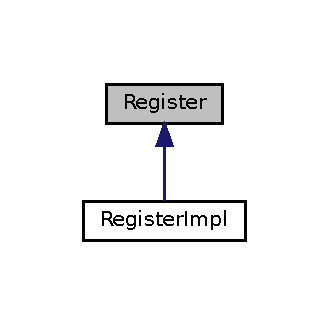
\includegraphics[width=158pt]{classRegister__inherit__graph}
\end{center}
\end{figure}
\subsection*{Public Member Functions}
\begin{DoxyCompactItemize}
\item 
virtual \hyperlink{classRegister_ab0464bc35e0902e33d35fff772548e74}{$\sim$\+Register} ()
\begin{DoxyCompactList}\small\item\em Destroy the \hyperlink{classRegister}{Register} object. \end{DoxyCompactList}\item 
virtual bool \hyperlink{classRegister_acfb8b5ecf7181faff5584765d78ab671}{create} (\hyperlink{classModel}{Model} $\ast$, string, string, string, string, const vector$<$ \hyperlink{classCourse}{Course} $\ast$$>$ \&, int)=0
\begin{DoxyCompactList}\small\item\em register an user \end{DoxyCompactList}\item 
virtual bool \hyperlink{classRegister_a09d7d6c24f7c07e97f7ef2d24a057f73}{remove} (\hyperlink{classModel}{Model} $\ast$, \hyperlink{classUser}{User} $\ast$)=0
\begin{DoxyCompactList}\small\item\em remove an user \end{DoxyCompactList}\item 
virtual void \hyperlink{classRegister_ae1ca8b9044dff27a840a3d26fd5ea323}{update} (\hyperlink{classModel}{Model} $\ast$, \hyperlink{classUser}{User} $\ast$, string, string, string, string, const vector$<$ \hyperlink{classCourse}{Course} $\ast$$>$ \&, int)=0
\begin{DoxyCompactList}\small\item\em update an user \end{DoxyCompactList}\item 
virtual bool \hyperlink{classRegister_a243b58e5f1747437bab5175927cce26f}{search} (\hyperlink{classModel}{Model} $\ast$, const string \&) const =0
\begin{DoxyCompactList}\small\item\em search an user \end{DoxyCompactList}\item 
virtual \hyperlink{classUser}{User} $\ast$ \hyperlink{classRegister_ae1cb0de5f04828c81d2dbad9650e1d6f}{consult} (\hyperlink{classModel}{Model} $\ast$, const string \&) const =0
\begin{DoxyCompactList}\small\item\em consult an user \end{DoxyCompactList}\item 
virtual bool \hyperlink{classRegister_aeeb9ead57f749601459240fc68cfe7b4}{Validate\+Email} (string)=0
\begin{DoxyCompactList}\small\item\em validate the user email \end{DoxyCompactList}\end{DoxyCompactItemize}
\subsection*{Static Public Member Functions}
\begin{DoxyCompactItemize}
\item 
static \hyperlink{classRegister}{Register} $\ast$ \hyperlink{classRegister_ae94e883032b0a13d28e1fba375894fb6}{create\+Register} ()
\begin{DoxyCompactList}\small\item\em Create a \hyperlink{classRegister}{Register} object. \end{DoxyCompactList}\end{DoxyCompactItemize}


\subsection{Detailed Description}
this class represents a register 

\subsection{Constructor \& Destructor Documentation}
\mbox{\Hypertarget{classRegister_ab0464bc35e0902e33d35fff772548e74}\label{classRegister_ab0464bc35e0902e33d35fff772548e74}} 
\index{Register@{Register}!````~Register@{$\sim$\+Register}}
\index{````~Register@{$\sim$\+Register}!Register@{Register}}
\subsubsection{\texorpdfstring{$\sim$\+Register()}{~Register()}}
{\footnotesize\ttfamily virtual Register\+::$\sim$\+Register (\begin{DoxyParamCaption}{ }\end{DoxyParamCaption})\hspace{0.3cm}{\ttfamily [inline]}, {\ttfamily [virtual]}}



Destroy the \hyperlink{classRegister}{Register} object. 



\subsection{Member Function Documentation}
\mbox{\Hypertarget{classRegister_ae1cb0de5f04828c81d2dbad9650e1d6f}\label{classRegister_ae1cb0de5f04828c81d2dbad9650e1d6f}} 
\index{Register@{Register}!consult@{consult}}
\index{consult@{consult}!Register@{Register}}
\subsubsection{\texorpdfstring{consult()}{consult()}}
{\footnotesize\ttfamily virtual \hyperlink{classUser}{User}$\ast$ Register\+::consult (\begin{DoxyParamCaption}\item[{\hyperlink{classModel}{Model} $\ast$}]{,  }\item[{const string \&}]{ }\end{DoxyParamCaption}) const\hspace{0.3cm}{\ttfamily [pure virtual]}}



consult an user 

\begin{DoxyReturn}{Returns}
User$\ast$ the user pointer 
\end{DoxyReturn}


Implemented in \hyperlink{classRegisterImpl_afe762d2896bb50b551e7b317c4936ac3}{Register\+Impl}.

\mbox{\Hypertarget{classRegister_acfb8b5ecf7181faff5584765d78ab671}\label{classRegister_acfb8b5ecf7181faff5584765d78ab671}} 
\index{Register@{Register}!create@{create}}
\index{create@{create}!Register@{Register}}
\subsubsection{\texorpdfstring{create()}{create()}}
{\footnotesize\ttfamily virtual bool Register\+::create (\begin{DoxyParamCaption}\item[{\hyperlink{classModel}{Model} $\ast$}]{,  }\item[{string}]{,  }\item[{string}]{,  }\item[{string}]{,  }\item[{string}]{,  }\item[{const vector$<$ \hyperlink{classCourse}{Course} $\ast$$>$ \&}]{,  }\item[{int}]{ }\end{DoxyParamCaption})\hspace{0.3cm}{\ttfamily [pure virtual]}}



register an user 

\begin{DoxyReturn}{Returns}
true if it was successful 

false if it failed 
\end{DoxyReturn}


Implemented in \hyperlink{classRegisterImpl_af0463a5627b02b797a4a9d5d90f55a46}{Register\+Impl}.

\mbox{\Hypertarget{classRegister_ae94e883032b0a13d28e1fba375894fb6}\label{classRegister_ae94e883032b0a13d28e1fba375894fb6}} 
\index{Register@{Register}!create\+Register@{create\+Register}}
\index{create\+Register@{create\+Register}!Register@{Register}}
\subsubsection{\texorpdfstring{create\+Register()}{createRegister()}}
{\footnotesize\ttfamily \hyperlink{classRegister}{Register} $\ast$ Register\+::create\+Register (\begin{DoxyParamCaption}{ }\end{DoxyParamCaption})\hspace{0.3cm}{\ttfamily [static]}}



Create a \hyperlink{classRegister}{Register} object. 

\begin{DoxyReturn}{Returns}
Register$\ast$ the register pointer 
\end{DoxyReturn}
\mbox{\Hypertarget{classRegister_a09d7d6c24f7c07e97f7ef2d24a057f73}\label{classRegister_a09d7d6c24f7c07e97f7ef2d24a057f73}} 
\index{Register@{Register}!remove@{remove}}
\index{remove@{remove}!Register@{Register}}
\subsubsection{\texorpdfstring{remove()}{remove()}}
{\footnotesize\ttfamily virtual bool Register\+::remove (\begin{DoxyParamCaption}\item[{\hyperlink{classModel}{Model} $\ast$}]{,  }\item[{\hyperlink{classUser}{User} $\ast$}]{ }\end{DoxyParamCaption})\hspace{0.3cm}{\ttfamily [pure virtual]}}



remove an user 

\begin{DoxyReturn}{Returns}
true if it was successful 

false if it failed 
\end{DoxyReturn}


Implemented in \hyperlink{classRegisterImpl_a528ea874f5607abfea9fea4b8cab1628}{Register\+Impl}.

\mbox{\Hypertarget{classRegister_a243b58e5f1747437bab5175927cce26f}\label{classRegister_a243b58e5f1747437bab5175927cce26f}} 
\index{Register@{Register}!search@{search}}
\index{search@{search}!Register@{Register}}
\subsubsection{\texorpdfstring{search()}{search()}}
{\footnotesize\ttfamily virtual bool Register\+::search (\begin{DoxyParamCaption}\item[{\hyperlink{classModel}{Model} $\ast$}]{,  }\item[{const string \&}]{ }\end{DoxyParamCaption}) const\hspace{0.3cm}{\ttfamily [pure virtual]}}



search an user 

\begin{DoxyReturn}{Returns}
true if it was successful 

false if it failed 
\end{DoxyReturn}


Implemented in \hyperlink{classRegisterImpl_ad60a7330160adae90443acb547398bd9}{Register\+Impl}.

\mbox{\Hypertarget{classRegister_ae1ca8b9044dff27a840a3d26fd5ea323}\label{classRegister_ae1ca8b9044dff27a840a3d26fd5ea323}} 
\index{Register@{Register}!update@{update}}
\index{update@{update}!Register@{Register}}
\subsubsection{\texorpdfstring{update()}{update()}}
{\footnotesize\ttfamily virtual void Register\+::update (\begin{DoxyParamCaption}\item[{\hyperlink{classModel}{Model} $\ast$}]{,  }\item[{\hyperlink{classUser}{User} $\ast$}]{,  }\item[{string}]{,  }\item[{string}]{,  }\item[{string}]{,  }\item[{string}]{,  }\item[{const vector$<$ \hyperlink{classCourse}{Course} $\ast$$>$ \&}]{,  }\item[{int}]{ }\end{DoxyParamCaption})\hspace{0.3cm}{\ttfamily [pure virtual]}}



update an user 



Implemented in \hyperlink{classRegisterImpl_a5ae0846ac09fe620501b94f5e05bcd9d}{Register\+Impl}.

\mbox{\Hypertarget{classRegister_aeeb9ead57f749601459240fc68cfe7b4}\label{classRegister_aeeb9ead57f749601459240fc68cfe7b4}} 
\index{Register@{Register}!Validate\+Email@{Validate\+Email}}
\index{Validate\+Email@{Validate\+Email}!Register@{Register}}
\subsubsection{\texorpdfstring{Validate\+Email()}{ValidateEmail()}}
{\footnotesize\ttfamily virtual bool Register\+::\+Validate\+Email (\begin{DoxyParamCaption}\item[{string}]{ }\end{DoxyParamCaption})\hspace{0.3cm}{\ttfamily [pure virtual]}}



validate the user email 

\begin{DoxyReturn}{Returns}
true if it was successful 

false if it failed 
\end{DoxyReturn}


Implemented in \hyperlink{classRegisterImpl_a3c0a7f6df3b0be5ce7fe8d7a78214304}{Register\+Impl}.



The documentation for this class was generated from the following files\+:\begin{DoxyCompactItemize}
\item 
src/lib/\hyperlink{register_8h}{register.\+h}\item 
src/lib/\hyperlink{register__impl_8cpp}{register\+\_\+impl.\+cpp}\end{DoxyCompactItemize}

\hypertarget{classRegisterImpl}{}\section{Register\+Impl Class Reference}
\label{classRegisterImpl}\index{Register\+Impl@{Register\+Impl}}


this class represents a register  




{\ttfamily \#include $<$register\+\_\+impl.\+h$>$}



Inheritance diagram for Register\+Impl\+:\nopagebreak
\begin{figure}[H]
\begin{center}
\leavevmode
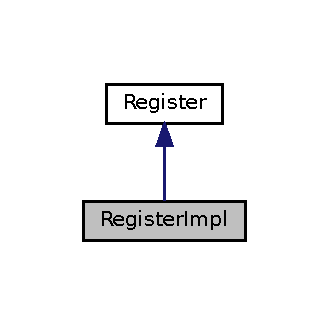
\includegraphics[width=158pt]{classRegisterImpl__inherit__graph}
\end{center}
\end{figure}


Collaboration diagram for Register\+Impl\+:\nopagebreak
\begin{figure}[H]
\begin{center}
\leavevmode
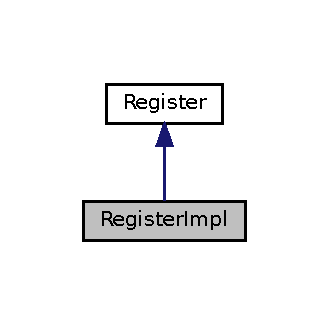
\includegraphics[width=158pt]{classRegisterImpl__coll__graph}
\end{center}
\end{figure}
\subsection*{Public Member Functions}
\begin{DoxyCompactItemize}
\item 
\hyperlink{classRegisterImpl_a601b77faf4f07f51170821a189fed94f}{Register\+Impl} ()
\begin{DoxyCompactList}\small\item\em Construct a new \hyperlink{classRegister}{Register} Impl object. \end{DoxyCompactList}\item 
\hyperlink{classRegisterImpl_ab227f612d7fdd113cab53c9559b0c8f9}{$\sim$\+Register\+Impl} ()
\begin{DoxyCompactList}\small\item\em Destroy the \hyperlink{classRegister}{Register} Impl object. \end{DoxyCompactList}\item 
bool \hyperlink{classRegisterImpl_af0463a5627b02b797a4a9d5d90f55a46}{create} (\hyperlink{classModel}{Model} $\ast$, string, string, string, string, const vector$<$ \hyperlink{classCourse}{Course} $\ast$$>$ \&, int)
\begin{DoxyCompactList}\small\item\em register an user \end{DoxyCompactList}\item 
bool \hyperlink{classRegisterImpl_a528ea874f5607abfea9fea4b8cab1628}{remove} (\hyperlink{classModel}{Model} $\ast$, \hyperlink{classUser}{User} $\ast$)
\begin{DoxyCompactList}\small\item\em remove an user \end{DoxyCompactList}\item 
void \hyperlink{classRegisterImpl_a5ae0846ac09fe620501b94f5e05bcd9d}{update} (\hyperlink{classModel}{Model} $\ast$, \hyperlink{classUser}{User} $\ast$, string, string, string, string, const vector$<$ \hyperlink{classCourse}{Course} $\ast$$>$ \&, int)
\begin{DoxyCompactList}\small\item\em update an user \end{DoxyCompactList}\item 
bool \hyperlink{classRegisterImpl_ad60a7330160adae90443acb547398bd9}{search} (\hyperlink{classModel}{Model} $\ast$, const string \&) const
\begin{DoxyCompactList}\small\item\em search an user \end{DoxyCompactList}\item 
\hyperlink{classUser}{User} $\ast$ \hyperlink{classRegisterImpl_afe762d2896bb50b551e7b317c4936ac3}{consult} (\hyperlink{classModel}{Model} $\ast$, const string \&) const
\begin{DoxyCompactList}\small\item\em consult an user \end{DoxyCompactList}\item 
bool \hyperlink{classRegisterImpl_a3c0a7f6df3b0be5ce7fe8d7a78214304}{Validate\+Email} (string)
\begin{DoxyCompactList}\small\item\em validate the user email \end{DoxyCompactList}\end{DoxyCompactItemize}
\subsection*{Static Public Member Functions}
\begin{DoxyCompactItemize}
\item 
static \hyperlink{classRegister}{Register} $\ast$ \hyperlink{classRegisterImpl_a505a9051efb8758a31da6ce97241741c}{create\+Register} ()
\begin{DoxyCompactList}\small\item\em Create a \hyperlink{classRegister}{Register} object. \end{DoxyCompactList}\end{DoxyCompactItemize}


\subsection{Detailed Description}
this class represents a register 

\subsection{Constructor \& Destructor Documentation}
\mbox{\Hypertarget{classRegisterImpl_a601b77faf4f07f51170821a189fed94f}\label{classRegisterImpl_a601b77faf4f07f51170821a189fed94f}} 
\index{Register\+Impl@{Register\+Impl}!Register\+Impl@{Register\+Impl}}
\index{Register\+Impl@{Register\+Impl}!Register\+Impl@{Register\+Impl}}
\subsubsection{\texorpdfstring{Register\+Impl()}{RegisterImpl()}}
{\footnotesize\ttfamily Register\+Impl\+::\+Register\+Impl (\begin{DoxyParamCaption}{ }\end{DoxyParamCaption})}



Construct a new \hyperlink{classRegister}{Register} Impl object. 

\mbox{\Hypertarget{classRegisterImpl_ab227f612d7fdd113cab53c9559b0c8f9}\label{classRegisterImpl_ab227f612d7fdd113cab53c9559b0c8f9}} 
\index{Register\+Impl@{Register\+Impl}!````~Register\+Impl@{$\sim$\+Register\+Impl}}
\index{````~Register\+Impl@{$\sim$\+Register\+Impl}!Register\+Impl@{Register\+Impl}}
\subsubsection{\texorpdfstring{$\sim$\+Register\+Impl()}{~RegisterImpl()}}
{\footnotesize\ttfamily Register\+Impl\+::$\sim$\+Register\+Impl (\begin{DoxyParamCaption}{ }\end{DoxyParamCaption})}



Destroy the \hyperlink{classRegister}{Register} Impl object. 



\subsection{Member Function Documentation}
\mbox{\Hypertarget{classRegisterImpl_afe762d2896bb50b551e7b317c4936ac3}\label{classRegisterImpl_afe762d2896bb50b551e7b317c4936ac3}} 
\index{Register\+Impl@{Register\+Impl}!consult@{consult}}
\index{consult@{consult}!Register\+Impl@{Register\+Impl}}
\subsubsection{\texorpdfstring{consult()}{consult()}}
{\footnotesize\ttfamily \hyperlink{classUser}{User} $\ast$ Register\+Impl\+::consult (\begin{DoxyParamCaption}\item[{\hyperlink{classModel}{Model} $\ast$}]{model,  }\item[{const string \&}]{name }\end{DoxyParamCaption}) const\hspace{0.3cm}{\ttfamily [virtual]}}



consult an user 

\begin{DoxyReturn}{Returns}
User$\ast$ the user pointer 
\end{DoxyReturn}


Implements \hyperlink{classRegister_ae1cb0de5f04828c81d2dbad9650e1d6f}{Register}.

\mbox{\Hypertarget{classRegisterImpl_af0463a5627b02b797a4a9d5d90f55a46}\label{classRegisterImpl_af0463a5627b02b797a4a9d5d90f55a46}} 
\index{Register\+Impl@{Register\+Impl}!create@{create}}
\index{create@{create}!Register\+Impl@{Register\+Impl}}
\subsubsection{\texorpdfstring{create()}{create()}}
{\footnotesize\ttfamily bool Register\+Impl\+::create (\begin{DoxyParamCaption}\item[{\hyperlink{classModel}{Model} $\ast$}]{model,  }\item[{string}]{name,  }\item[{string}]{email,  }\item[{string}]{cpf,  }\item[{string}]{password,  }\item[{const vector$<$ \hyperlink{classCourse}{Course} $\ast$$>$ \&}]{courses,  }\item[{int}]{permission }\end{DoxyParamCaption})\hspace{0.3cm}{\ttfamily [virtual]}}



register an user 

\begin{DoxyReturn}{Returns}
true if it was successful 

false if it failed 
\end{DoxyReturn}


Implements \hyperlink{classRegister_acfb8b5ecf7181faff5584765d78ab671}{Register}.

\mbox{\Hypertarget{classRegisterImpl_a505a9051efb8758a31da6ce97241741c}\label{classRegisterImpl_a505a9051efb8758a31da6ce97241741c}} 
\index{Register\+Impl@{Register\+Impl}!create\+Register@{create\+Register}}
\index{create\+Register@{create\+Register}!Register\+Impl@{Register\+Impl}}
\subsubsection{\texorpdfstring{create\+Register()}{createRegister()}}
{\footnotesize\ttfamily \hyperlink{classRegister}{Register} $\ast$ Register\+Impl\+::create\+Register (\begin{DoxyParamCaption}{ }\end{DoxyParamCaption})\hspace{0.3cm}{\ttfamily [static]}}



Create a \hyperlink{classRegister}{Register} object. 

\begin{DoxyReturn}{Returns}
Register$\ast$ the register pointer 
\end{DoxyReturn}
\mbox{\Hypertarget{classRegisterImpl_a528ea874f5607abfea9fea4b8cab1628}\label{classRegisterImpl_a528ea874f5607abfea9fea4b8cab1628}} 
\index{Register\+Impl@{Register\+Impl}!remove@{remove}}
\index{remove@{remove}!Register\+Impl@{Register\+Impl}}
\subsubsection{\texorpdfstring{remove()}{remove()}}
{\footnotesize\ttfamily bool Register\+Impl\+::remove (\begin{DoxyParamCaption}\item[{\hyperlink{classModel}{Model} $\ast$}]{model,  }\item[{\hyperlink{classUser}{User} $\ast$}]{user }\end{DoxyParamCaption})\hspace{0.3cm}{\ttfamily [virtual]}}



remove an user 

\begin{DoxyReturn}{Returns}
true if it was successful 

false if it failed 
\end{DoxyReturn}


Implements \hyperlink{classRegister_a09d7d6c24f7c07e97f7ef2d24a057f73}{Register}.

\mbox{\Hypertarget{classRegisterImpl_ad60a7330160adae90443acb547398bd9}\label{classRegisterImpl_ad60a7330160adae90443acb547398bd9}} 
\index{Register\+Impl@{Register\+Impl}!search@{search}}
\index{search@{search}!Register\+Impl@{Register\+Impl}}
\subsubsection{\texorpdfstring{search()}{search()}}
{\footnotesize\ttfamily bool Register\+Impl\+::search (\begin{DoxyParamCaption}\item[{\hyperlink{classModel}{Model} $\ast$}]{model,  }\item[{const string \&}]{name }\end{DoxyParamCaption}) const\hspace{0.3cm}{\ttfamily [virtual]}}



search an user 

\begin{DoxyReturn}{Returns}
true if it was successful 

false if it failed 
\end{DoxyReturn}


Implements \hyperlink{classRegister_a243b58e5f1747437bab5175927cce26f}{Register}.

\mbox{\Hypertarget{classRegisterImpl_a5ae0846ac09fe620501b94f5e05bcd9d}\label{classRegisterImpl_a5ae0846ac09fe620501b94f5e05bcd9d}} 
\index{Register\+Impl@{Register\+Impl}!update@{update}}
\index{update@{update}!Register\+Impl@{Register\+Impl}}
\subsubsection{\texorpdfstring{update()}{update()}}
{\footnotesize\ttfamily void Register\+Impl\+::update (\begin{DoxyParamCaption}\item[{\hyperlink{classModel}{Model} $\ast$}]{model,  }\item[{\hyperlink{classUser}{User} $\ast$}]{user,  }\item[{string}]{name,  }\item[{string}]{email,  }\item[{string}]{cpf,  }\item[{string}]{password,  }\item[{const vector$<$ \hyperlink{classCourse}{Course} $\ast$$>$ \&}]{courses,  }\item[{int}]{permission }\end{DoxyParamCaption})\hspace{0.3cm}{\ttfamily [virtual]}}



update an user 



Implements \hyperlink{classRegister_ae1ca8b9044dff27a840a3d26fd5ea323}{Register}.

\mbox{\Hypertarget{classRegisterImpl_a3c0a7f6df3b0be5ce7fe8d7a78214304}\label{classRegisterImpl_a3c0a7f6df3b0be5ce7fe8d7a78214304}} 
\index{Register\+Impl@{Register\+Impl}!Validate\+Email@{Validate\+Email}}
\index{Validate\+Email@{Validate\+Email}!Register\+Impl@{Register\+Impl}}
\subsubsection{\texorpdfstring{Validate\+Email()}{ValidateEmail()}}
{\footnotesize\ttfamily bool Register\+Impl\+::\+Validate\+Email (\begin{DoxyParamCaption}\item[{string}]{email }\end{DoxyParamCaption})\hspace{0.3cm}{\ttfamily [virtual]}}



validate the user email 

\begin{DoxyReturn}{Returns}
true if it was successful 

false if it failed 
\end{DoxyReturn}


Implements \hyperlink{classRegister_aeeb9ead57f749601459240fc68cfe7b4}{Register}.



The documentation for this class was generated from the following files\+:\begin{DoxyCompactItemize}
\item 
src/lib/\hyperlink{register__impl_8h}{register\+\_\+impl.\+h}\item 
src/lib/\hyperlink{register__impl_8cpp}{register\+\_\+impl.\+cpp}\end{DoxyCompactItemize}

\hypertarget{classregisterview}{}\section{registerview Class Reference}
\label{classregisterview}\index{registerview@{registerview}}


this class representer a Register\+View UI  




{\ttfamily \#include $<$registerview.\+h$>$}



Inheritance diagram for registerview\+:
\nopagebreak
\begin{figure}[H]
\begin{center}
\leavevmode
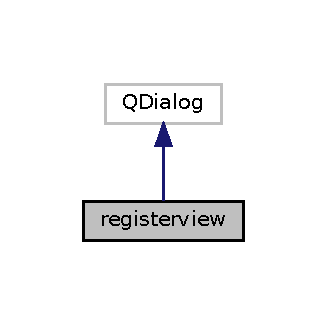
\includegraphics[width=157pt]{classregisterview__inherit__graph}
\end{center}
\end{figure}


Collaboration diagram for registerview\+:
\nopagebreak
\begin{figure}[H]
\begin{center}
\leavevmode
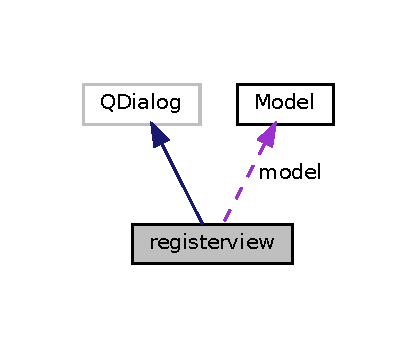
\includegraphics[width=200pt]{classregisterview__coll__graph}
\end{center}
\end{figure}
\subsection*{Public Member Functions}
\begin{DoxyCompactItemize}
\item 
\hyperlink{classregisterview_ad900dd927edcbdf6a134da28df5a83c6}{registerview} (Q\+Widget $\ast$parent=nullptr)
\begin{DoxyCompactList}\small\item\em Construct a new \hyperlink{classRegister}{Register} View object. \end{DoxyCompactList}\item 
\hyperlink{classregisterview_a824fc1c7f2c9a8e62aad92be80d381c6}{$\sim$registerview} ()
\begin{DoxyCompactList}\small\item\em Destroy the \hyperlink{classRegister}{Register} View object. \end{DoxyCompactList}\item 
\hyperlink{classModel}{Model} $\ast$ \hyperlink{classregisterview_a765c4046d743e6f3908615535c16eef1}{get\+Model} () const
\begin{DoxyCompactList}\small\item\em Get the \hyperlink{classModel}{Model} object. \end{DoxyCompactList}\item 
void \hyperlink{classregisterview_ae6d6efee19c05f34f6e1c778f2a76ec7}{set\+Model} (\hyperlink{classModel}{Model} $\ast$)
\begin{DoxyCompactList}\small\item\em Set the \hyperlink{classModel}{Model} object. \end{DoxyCompactList}\end{DoxyCompactItemize}
\subsection*{Private Slots}
\begin{DoxyCompactItemize}
\item 
void \hyperlink{classregisterview_a5541faebc6701e8e2da6a4c107cd4b0e}{on\+\_\+btn\+\_\+cancel\+\_\+clicked} ()
\begin{DoxyCompactList}\small\item\em the button function to cancel the operation \end{DoxyCompactList}\item 
void \hyperlink{classregisterview_adafbe9fb4f180f8badc6dd9788bbcf15}{on\+\_\+btn\+\_\+register\+\_\+clicked} ()
\begin{DoxyCompactList}\small\item\em the button function to register a user \end{DoxyCompactList}\end{DoxyCompactItemize}
\subsection*{Private Attributes}
\begin{DoxyCompactItemize}
\item 
Ui\+::registerview $\ast$ \hyperlink{classregisterview_ac8bc2dae39fb31c3bfe66f3c1ca07e59}{ui}
\item 
\hyperlink{classModel}{Model} $\ast$ \hyperlink{classregisterview_a1c8d39e08edad26afdfd16182189ee6c}{model}
\end{DoxyCompactItemize}


\subsection{Detailed Description}
this class representer a Register\+View UI 

\subsection{Constructor \& Destructor Documentation}
\mbox{\Hypertarget{classregisterview_ad900dd927edcbdf6a134da28df5a83c6}\label{classregisterview_ad900dd927edcbdf6a134da28df5a83c6}} 
\index{registerview@{registerview}!registerview@{registerview}}
\index{registerview@{registerview}!registerview@{registerview}}
\subsubsection{\texorpdfstring{registerview()}{registerview()}}
{\footnotesize\ttfamily registerview\+::registerview (\begin{DoxyParamCaption}\item[{Q\+Widget $\ast$}]{parent = {\ttfamily nullptr} }\end{DoxyParamCaption})\hspace{0.3cm}{\ttfamily [explicit]}}



Construct a new \hyperlink{classRegister}{Register} View object. 


\begin{DoxyParams}{Parameters}
{\em parent} & \\
\hline
\end{DoxyParams}
\mbox{\Hypertarget{classregisterview_a824fc1c7f2c9a8e62aad92be80d381c6}\label{classregisterview_a824fc1c7f2c9a8e62aad92be80d381c6}} 
\index{registerview@{registerview}!````~registerview@{$\sim$registerview}}
\index{````~registerview@{$\sim$registerview}!registerview@{registerview}}
\subsubsection{\texorpdfstring{$\sim$registerview()}{~registerview()}}
{\footnotesize\ttfamily registerview\+::$\sim$registerview (\begin{DoxyParamCaption}{ }\end{DoxyParamCaption})}



Destroy the \hyperlink{classRegister}{Register} View object. 



\subsection{Member Function Documentation}
\mbox{\Hypertarget{classregisterview_a765c4046d743e6f3908615535c16eef1}\label{classregisterview_a765c4046d743e6f3908615535c16eef1}} 
\index{registerview@{registerview}!get\+Model@{get\+Model}}
\index{get\+Model@{get\+Model}!registerview@{registerview}}
\subsubsection{\texorpdfstring{get\+Model()}{getModel()}}
{\footnotesize\ttfamily \hyperlink{classModel}{Model} $\ast$ registerview\+::get\+Model (\begin{DoxyParamCaption}{ }\end{DoxyParamCaption}) const}



Get the \hyperlink{classModel}{Model} object. 

\begin{DoxyReturn}{Returns}
Model$\ast$ the model pointer 
\end{DoxyReturn}
\mbox{\Hypertarget{classregisterview_a5541faebc6701e8e2da6a4c107cd4b0e}\label{classregisterview_a5541faebc6701e8e2da6a4c107cd4b0e}} 
\index{registerview@{registerview}!on\+\_\+btn\+\_\+cancel\+\_\+clicked@{on\+\_\+btn\+\_\+cancel\+\_\+clicked}}
\index{on\+\_\+btn\+\_\+cancel\+\_\+clicked@{on\+\_\+btn\+\_\+cancel\+\_\+clicked}!registerview@{registerview}}
\subsubsection{\texorpdfstring{on\+\_\+btn\+\_\+cancel\+\_\+clicked}{on\_btn\_cancel\_clicked}}
{\footnotesize\ttfamily void registerview\+::on\+\_\+btn\+\_\+cancel\+\_\+clicked (\begin{DoxyParamCaption}{ }\end{DoxyParamCaption})\hspace{0.3cm}{\ttfamily [private]}, {\ttfamily [slot]}}



the button function to cancel the operation 

\mbox{\Hypertarget{classregisterview_adafbe9fb4f180f8badc6dd9788bbcf15}\label{classregisterview_adafbe9fb4f180f8badc6dd9788bbcf15}} 
\index{registerview@{registerview}!on\+\_\+btn\+\_\+register\+\_\+clicked@{on\+\_\+btn\+\_\+register\+\_\+clicked}}
\index{on\+\_\+btn\+\_\+register\+\_\+clicked@{on\+\_\+btn\+\_\+register\+\_\+clicked}!registerview@{registerview}}
\subsubsection{\texorpdfstring{on\+\_\+btn\+\_\+register\+\_\+clicked}{on\_btn\_register\_clicked}}
{\footnotesize\ttfamily void registerview\+::on\+\_\+btn\+\_\+register\+\_\+clicked (\begin{DoxyParamCaption}{ }\end{DoxyParamCaption})\hspace{0.3cm}{\ttfamily [private]}, {\ttfamily [slot]}}



the button function to register a user 

\mbox{\Hypertarget{classregisterview_ae6d6efee19c05f34f6e1c778f2a76ec7}\label{classregisterview_ae6d6efee19c05f34f6e1c778f2a76ec7}} 
\index{registerview@{registerview}!set\+Model@{set\+Model}}
\index{set\+Model@{set\+Model}!registerview@{registerview}}
\subsubsection{\texorpdfstring{set\+Model()}{setModel()}}
{\footnotesize\ttfamily void registerview\+::set\+Model (\begin{DoxyParamCaption}\item[{\hyperlink{classModel}{Model} $\ast$}]{value }\end{DoxyParamCaption})}



Set the \hyperlink{classModel}{Model} object. 



\subsection{Member Data Documentation}
\mbox{\Hypertarget{classregisterview_a1c8d39e08edad26afdfd16182189ee6c}\label{classregisterview_a1c8d39e08edad26afdfd16182189ee6c}} 
\index{registerview@{registerview}!model@{model}}
\index{model@{model}!registerview@{registerview}}
\subsubsection{\texorpdfstring{model}{model}}
{\footnotesize\ttfamily \hyperlink{classModel}{Model}$\ast$ registerview\+::model\hspace{0.3cm}{\ttfamily [private]}}

\mbox{\Hypertarget{classregisterview_ac8bc2dae39fb31c3bfe66f3c1ca07e59}\label{classregisterview_ac8bc2dae39fb31c3bfe66f3c1ca07e59}} 
\index{registerview@{registerview}!ui@{ui}}
\index{ui@{ui}!registerview@{registerview}}
\subsubsection{\texorpdfstring{ui}{ui}}
{\footnotesize\ttfamily Ui\+::registerview$\ast$ registerview\+::ui\hspace{0.3cm}{\ttfamily [private]}}



The documentation for this class was generated from the following files\+:\begin{DoxyCompactItemize}
\item 
views/\hyperlink{registerview_8h}{registerview.\+h}\item 
views/\hyperlink{registerview_8cpp}{registerview.\+cpp}\end{DoxyCompactItemize}

\hypertarget{classUser}{}\section{User Class Reference}
\label{classUser}\index{User@{User}}


this class represents an user  




{\ttfamily \#include $<$user.\+h$>$}



Inheritance diagram for User\+:\nopagebreak
\begin{figure}[H]
\begin{center}
\leavevmode
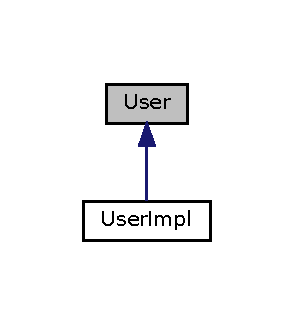
\includegraphics[width=141pt]{classUser__inherit__graph}
\end{center}
\end{figure}
\subsection*{Public Member Functions}
\begin{DoxyCompactItemize}
\item 
virtual \hyperlink{classUser_a7d1cf7c22ba031caec015ec427419513}{$\sim$\+User} ()
\begin{DoxyCompactList}\small\item\em Destroy the \hyperlink{classUser}{User} object. \end{DoxyCompactList}\item 
virtual string \hyperlink{classUser_a10b64aca04c37b66fcb5a112e87f97ac}{get\+Name} () const =0
\begin{DoxyCompactList}\small\item\em Get the Name fobject. \end{DoxyCompactList}\item 
virtual void \hyperlink{classUser_a47339f4f166d9baa023fdd59e81c965d}{set\+Name} (const string \&)=0
\begin{DoxyCompactList}\small\item\em Set the Name object. \end{DoxyCompactList}\item 
virtual string \hyperlink{classUser_a58eae5ae9bc079ca5ee31c41326b229e}{get\+Email} () const =0
\begin{DoxyCompactList}\small\item\em Get the Email object. \end{DoxyCompactList}\item 
virtual void \hyperlink{classUser_ac72e220fdcbb3decc392d2729f27e6b5}{set\+Email} (const string \&)=0
\begin{DoxyCompactList}\small\item\em Set the Email object. \end{DoxyCompactList}\item 
virtual string \hyperlink{classUser_a2a23ddf63962cdb3d8cef2054a0a27a0}{get\+C\+PF} () const =0
\begin{DoxyCompactList}\small\item\em Get the Birth object. \end{DoxyCompactList}\item 
virtual void \hyperlink{classUser_ac10d34adddaa80cb544eab7c5b1227f5}{set\+C\+PF} (const string \&)=0
\begin{DoxyCompactList}\small\item\em Set the Birth object. \end{DoxyCompactList}\item 
virtual string \hyperlink{classUser_a29d4b884ba9f2a3f28a77368c86239fd}{get\+Password} () const =0
\begin{DoxyCompactList}\small\item\em Get the Password object. \end{DoxyCompactList}\item 
virtual void \hyperlink{classUser_a809c17ec3427917ae2e641d171cb99d2}{set\+Password} (const string \&)=0
\begin{DoxyCompactList}\small\item\em Set the Password object. \end{DoxyCompactList}\item 
virtual vector$<$ \hyperlink{classCourse}{Course} $\ast$ $>$ \& \hyperlink{classUser_a72be855a1f58cc705591413a72a8e346}{get\+Courses} ()=0
\begin{DoxyCompactList}\small\item\em Get the Courses object. \end{DoxyCompactList}\item 
virtual void \hyperlink{classUser_a1b97c41fca71b2839d8acc57e9d006b2}{set\+Courses} (const vector$<$ \hyperlink{classCourse}{Course} $\ast$$>$ \&)=0
\begin{DoxyCompactList}\small\item\em Set the Courses object. \end{DoxyCompactList}\item 
virtual int \hyperlink{classUser_ae326f0c51a673f749ed57b9f0d0b723a}{get\+Permission} () const =0
\begin{DoxyCompactList}\small\item\em Get the Permission object. \end{DoxyCompactList}\item 
virtual void \hyperlink{classUser_ab6a6689e3581c70af166b2eb537df6fb}{set\+Permission} (int)=0
\begin{DoxyCompactList}\small\item\em Set the Permission object. \end{DoxyCompactList}\item 
virtual \hyperlink{classUser}{User} \& \hyperlink{classUser_afd7134b455781d42362cf5fd0d5d2e68}{operator=} (\hyperlink{classUser}{User} \&)=0
\begin{DoxyCompactList}\small\item\em assignment operator \end{DoxyCompactList}\item 
virtual bool \hyperlink{classUser_a461783a03e5a694a2cdd80fba7b18459}{operator==} (\hyperlink{classUser}{User} \&)=0
\begin{DoxyCompactList}\small\item\em association operator \end{DoxyCompactList}\end{DoxyCompactItemize}


\subsection{Detailed Description}
this class represents an user 

\subsection{Constructor \& Destructor Documentation}
\mbox{\Hypertarget{classUser_a7d1cf7c22ba031caec015ec427419513}\label{classUser_a7d1cf7c22ba031caec015ec427419513}} 
\index{User@{User}!````~User@{$\sim$\+User}}
\index{````~User@{$\sim$\+User}!User@{User}}
\subsubsection{\texorpdfstring{$\sim$\+User()}{~User()}}
{\footnotesize\ttfamily virtual User\+::$\sim$\+User (\begin{DoxyParamCaption}{ }\end{DoxyParamCaption})\hspace{0.3cm}{\ttfamily [inline]}, {\ttfamily [virtual]}}



Destroy the \hyperlink{classUser}{User} object. 



\subsection{Member Function Documentation}
\mbox{\Hypertarget{classUser_a72be855a1f58cc705591413a72a8e346}\label{classUser_a72be855a1f58cc705591413a72a8e346}} 
\index{User@{User}!get\+Courses@{get\+Courses}}
\index{get\+Courses@{get\+Courses}!User@{User}}
\subsubsection{\texorpdfstring{get\+Courses()}{getCourses()}}
{\footnotesize\ttfamily virtual vector$<$\hyperlink{classCourse}{Course}$\ast$$>$\& User\+::get\+Courses (\begin{DoxyParamCaption}{ }\end{DoxyParamCaption})\hspace{0.3cm}{\ttfamily [pure virtual]}}



Get the Courses object. 

\begin{DoxyReturn}{Returns}
vector$<$\+Course$\ast$$>$\& the user courses 
\end{DoxyReturn}


Implemented in \hyperlink{classUserImpl_aaac79e7ca4bf050cf0c180fb5ec2d751}{User\+Impl}.

\mbox{\Hypertarget{classUser_a2a23ddf63962cdb3d8cef2054a0a27a0}\label{classUser_a2a23ddf63962cdb3d8cef2054a0a27a0}} 
\index{User@{User}!get\+C\+PF@{get\+C\+PF}}
\index{get\+C\+PF@{get\+C\+PF}!User@{User}}
\subsubsection{\texorpdfstring{get\+C\+P\+F()}{getCPF()}}
{\footnotesize\ttfamily virtual string User\+::get\+C\+PF (\begin{DoxyParamCaption}{ }\end{DoxyParamCaption}) const\hspace{0.3cm}{\ttfamily [pure virtual]}}



Get the Birth object. 

\begin{DoxyReturn}{Returns}
string the user birthday 
\end{DoxyReturn}


Implemented in \hyperlink{classUserImpl_aa20a69738aa1b1ee2e04a6aa65833440}{User\+Impl}.

\mbox{\Hypertarget{classUser_a58eae5ae9bc079ca5ee31c41326b229e}\label{classUser_a58eae5ae9bc079ca5ee31c41326b229e}} 
\index{User@{User}!get\+Email@{get\+Email}}
\index{get\+Email@{get\+Email}!User@{User}}
\subsubsection{\texorpdfstring{get\+Email()}{getEmail()}}
{\footnotesize\ttfamily virtual string User\+::get\+Email (\begin{DoxyParamCaption}{ }\end{DoxyParamCaption}) const\hspace{0.3cm}{\ttfamily [pure virtual]}}



Get the Email object. 

\begin{DoxyReturn}{Returns}
string the user email 
\end{DoxyReturn}


Implemented in \hyperlink{classUserImpl_add6a78d438f5dc401b220c39c7d40a61}{User\+Impl}.

\mbox{\Hypertarget{classUser_a10b64aca04c37b66fcb5a112e87f97ac}\label{classUser_a10b64aca04c37b66fcb5a112e87f97ac}} 
\index{User@{User}!get\+Name@{get\+Name}}
\index{get\+Name@{get\+Name}!User@{User}}
\subsubsection{\texorpdfstring{get\+Name()}{getName()}}
{\footnotesize\ttfamily virtual string User\+::get\+Name (\begin{DoxyParamCaption}{ }\end{DoxyParamCaption}) const\hspace{0.3cm}{\ttfamily [pure virtual]}}



Get the Name fobject. 

\begin{DoxyReturn}{Returns}
string the user name 
\end{DoxyReturn}


Implemented in \hyperlink{classUserImpl_afb305ca89d0de723270de3433e3b5fc1}{User\+Impl}.

\mbox{\Hypertarget{classUser_a29d4b884ba9f2a3f28a77368c86239fd}\label{classUser_a29d4b884ba9f2a3f28a77368c86239fd}} 
\index{User@{User}!get\+Password@{get\+Password}}
\index{get\+Password@{get\+Password}!User@{User}}
\subsubsection{\texorpdfstring{get\+Password()}{getPassword()}}
{\footnotesize\ttfamily virtual string User\+::get\+Password (\begin{DoxyParamCaption}{ }\end{DoxyParamCaption}) const\hspace{0.3cm}{\ttfamily [pure virtual]}}



Get the Password object. 

\begin{DoxyReturn}{Returns}
string the user password 
\end{DoxyReturn}


Implemented in \hyperlink{classUserImpl_a984ad7c34f6893ad4c06bb7d31b0afb0}{User\+Impl}.

\mbox{\Hypertarget{classUser_ae326f0c51a673f749ed57b9f0d0b723a}\label{classUser_ae326f0c51a673f749ed57b9f0d0b723a}} 
\index{User@{User}!get\+Permission@{get\+Permission}}
\index{get\+Permission@{get\+Permission}!User@{User}}
\subsubsection{\texorpdfstring{get\+Permission()}{getPermission()}}
{\footnotesize\ttfamily virtual int User\+::get\+Permission (\begin{DoxyParamCaption}{ }\end{DoxyParamCaption}) const\hspace{0.3cm}{\ttfamily [pure virtual]}}



Get the Permission object. 

\begin{DoxyReturn}{Returns}
int the user permission level 
\end{DoxyReturn}


Implemented in \hyperlink{classUserImpl_ac2233b5f85222b2db6a1877083374973}{User\+Impl}.

\mbox{\Hypertarget{classUser_afd7134b455781d42362cf5fd0d5d2e68}\label{classUser_afd7134b455781d42362cf5fd0d5d2e68}} 
\index{User@{User}!operator=@{operator=}}
\index{operator=@{operator=}!User@{User}}
\subsubsection{\texorpdfstring{operator=()}{operator=()}}
{\footnotesize\ttfamily virtual \hyperlink{classUser}{User}\& User\+::operator= (\begin{DoxyParamCaption}\item[{\hyperlink{classUser}{User} \&}]{ }\end{DoxyParamCaption})\hspace{0.3cm}{\ttfamily [pure virtual]}}



assignment operator 

\begin{DoxyReturn}{Returns}
\hyperlink{classUser}{User}\& the user reference 
\end{DoxyReturn}


Implemented in \hyperlink{classUserImpl_aa89ed62b1dbd34811cf7e32137009b6d}{User\+Impl}.

\mbox{\Hypertarget{classUser_a461783a03e5a694a2cdd80fba7b18459}\label{classUser_a461783a03e5a694a2cdd80fba7b18459}} 
\index{User@{User}!operator==@{operator==}}
\index{operator==@{operator==}!User@{User}}
\subsubsection{\texorpdfstring{operator==()}{operator==()}}
{\footnotesize\ttfamily virtual bool User\+::operator== (\begin{DoxyParamCaption}\item[{\hyperlink{classUser}{User} \&}]{ }\end{DoxyParamCaption})\hspace{0.3cm}{\ttfamily [pure virtual]}}



association operator 

\begin{DoxyReturn}{Returns}
true if it was successful 

false if it failed 
\end{DoxyReturn}


Implemented in \hyperlink{classUserImpl_a1b79e70d839345e3ea0b05637183c1e1}{User\+Impl}.

\mbox{\Hypertarget{classUser_a1b97c41fca71b2839d8acc57e9d006b2}\label{classUser_a1b97c41fca71b2839d8acc57e9d006b2}} 
\index{User@{User}!set\+Courses@{set\+Courses}}
\index{set\+Courses@{set\+Courses}!User@{User}}
\subsubsection{\texorpdfstring{set\+Courses()}{setCourses()}}
{\footnotesize\ttfamily virtual void User\+::set\+Courses (\begin{DoxyParamCaption}\item[{const vector$<$ \hyperlink{classCourse}{Course} $\ast$$>$ \&}]{ }\end{DoxyParamCaption})\hspace{0.3cm}{\ttfamily [pure virtual]}}



Set the Courses object. 



Implemented in \hyperlink{classUserImpl_a0b01431638678ab1f7e39202c2374e4e}{User\+Impl}.

\mbox{\Hypertarget{classUser_ac10d34adddaa80cb544eab7c5b1227f5}\label{classUser_ac10d34adddaa80cb544eab7c5b1227f5}} 
\index{User@{User}!set\+C\+PF@{set\+C\+PF}}
\index{set\+C\+PF@{set\+C\+PF}!User@{User}}
\subsubsection{\texorpdfstring{set\+C\+P\+F()}{setCPF()}}
{\footnotesize\ttfamily virtual void User\+::set\+C\+PF (\begin{DoxyParamCaption}\item[{const string \&}]{ }\end{DoxyParamCaption})\hspace{0.3cm}{\ttfamily [pure virtual]}}



Set the Birth object. 



Implemented in \hyperlink{classUserImpl_a9964fc4ed651ce945f663cb4df8e042b}{User\+Impl}.

\mbox{\Hypertarget{classUser_ac72e220fdcbb3decc392d2729f27e6b5}\label{classUser_ac72e220fdcbb3decc392d2729f27e6b5}} 
\index{User@{User}!set\+Email@{set\+Email}}
\index{set\+Email@{set\+Email}!User@{User}}
\subsubsection{\texorpdfstring{set\+Email()}{setEmail()}}
{\footnotesize\ttfamily virtual void User\+::set\+Email (\begin{DoxyParamCaption}\item[{const string \&}]{ }\end{DoxyParamCaption})\hspace{0.3cm}{\ttfamily [pure virtual]}}



Set the Email object. 



Implemented in \hyperlink{classUserImpl_abbd8347c11bd2ea93d37ec123b42dc6b}{User\+Impl}.

\mbox{\Hypertarget{classUser_a47339f4f166d9baa023fdd59e81c965d}\label{classUser_a47339f4f166d9baa023fdd59e81c965d}} 
\index{User@{User}!set\+Name@{set\+Name}}
\index{set\+Name@{set\+Name}!User@{User}}
\subsubsection{\texorpdfstring{set\+Name()}{setName()}}
{\footnotesize\ttfamily virtual void User\+::set\+Name (\begin{DoxyParamCaption}\item[{const string \&}]{ }\end{DoxyParamCaption})\hspace{0.3cm}{\ttfamily [pure virtual]}}



Set the Name object. 



Implemented in \hyperlink{classUserImpl_a30507ad79190a2ad7d896b6c4a55fab4}{User\+Impl}.

\mbox{\Hypertarget{classUser_a809c17ec3427917ae2e641d171cb99d2}\label{classUser_a809c17ec3427917ae2e641d171cb99d2}} 
\index{User@{User}!set\+Password@{set\+Password}}
\index{set\+Password@{set\+Password}!User@{User}}
\subsubsection{\texorpdfstring{set\+Password()}{setPassword()}}
{\footnotesize\ttfamily virtual void User\+::set\+Password (\begin{DoxyParamCaption}\item[{const string \&}]{ }\end{DoxyParamCaption})\hspace{0.3cm}{\ttfamily [pure virtual]}}



Set the Password object. 



Implemented in \hyperlink{classUserImpl_a85b0f1b2faebc315a2f5e4a128137101}{User\+Impl}.

\mbox{\Hypertarget{classUser_ab6a6689e3581c70af166b2eb537df6fb}\label{classUser_ab6a6689e3581c70af166b2eb537df6fb}} 
\index{User@{User}!set\+Permission@{set\+Permission}}
\index{set\+Permission@{set\+Permission}!User@{User}}
\subsubsection{\texorpdfstring{set\+Permission()}{setPermission()}}
{\footnotesize\ttfamily virtual void User\+::set\+Permission (\begin{DoxyParamCaption}\item[{int}]{ }\end{DoxyParamCaption})\hspace{0.3cm}{\ttfamily [pure virtual]}}



Set the Permission object. 



Implemented in \hyperlink{classUserImpl_ac273d611344f59bf69e6eabb412e84ee}{User\+Impl}.



The documentation for this class was generated from the following file\+:\begin{DoxyCompactItemize}
\item 
src/classes/\hyperlink{user_8h}{user.\+h}\end{DoxyCompactItemize}

\hypertarget{classUserImpl}{}\section{User\+Impl Class Reference}
\label{classUserImpl}\index{User\+Impl@{User\+Impl}}


this class represents an user  




{\ttfamily \#include $<$user\+\_\+impl.\+h$>$}



Inheritance diagram for User\+Impl\+:
\nopagebreak
\begin{figure}[H]
\begin{center}
\leavevmode
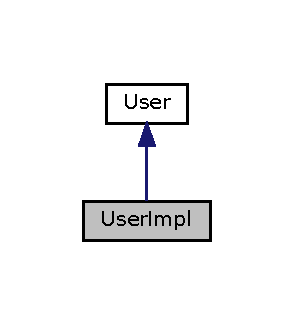
\includegraphics[width=141pt]{classUserImpl__inherit__graph}
\end{center}
\end{figure}


Collaboration diagram for User\+Impl\+:
\nopagebreak
\begin{figure}[H]
\begin{center}
\leavevmode
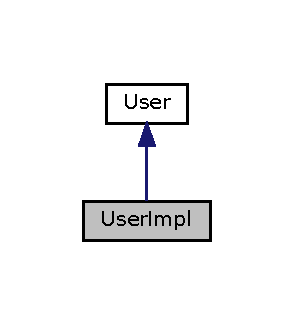
\includegraphics[width=141pt]{classUserImpl__coll__graph}
\end{center}
\end{figure}
\subsection*{Public Member Functions}
\begin{DoxyCompactItemize}
\item 
\hyperlink{classUserImpl_a247633b3d3fb9449719bd9c12873b4cb}{User\+Impl} ()
\begin{DoxyCompactList}\small\item\em Construct a new \hyperlink{classUser}{User} Impl object. \end{DoxyCompactList}\item 
\hyperlink{classUserImpl_a5c9de4c05578de165fe9c7b8d2138831}{User\+Impl} (\hyperlink{classUser}{User} $\ast$)
\begin{DoxyCompactList}\small\item\em Construct a new \hyperlink{classUser}{User} Impl object. \end{DoxyCompactList}\item 
\hyperlink{classUserImpl_a54977619bd2174542f04de58ec932fb5}{User\+Impl} (string, string, string, string, const vector$<$ \hyperlink{classCourse}{Course} $\ast$$>$ \&, int)
\begin{DoxyCompactList}\small\item\em Construct a new \hyperlink{classUser}{User} Impl object. \end{DoxyCompactList}\item 
\hyperlink{classUserImpl_ad138e8fe61218dbbe61a13ce9b17decc}{$\sim$\+User\+Impl} ()
\begin{DoxyCompactList}\small\item\em Destroy the \hyperlink{classUser}{User} Impl object. \end{DoxyCompactList}\item 
string \hyperlink{classUserImpl_afb305ca89d0de723270de3433e3b5fc1}{get\+Name} () const
\begin{DoxyCompactList}\small\item\em Get the Name object. \end{DoxyCompactList}\item 
void \hyperlink{classUserImpl_a30507ad79190a2ad7d896b6c4a55fab4}{set\+Name} (const string \&)
\begin{DoxyCompactList}\small\item\em Set the Name object. \end{DoxyCompactList}\item 
string \hyperlink{classUserImpl_add6a78d438f5dc401b220c39c7d40a61}{get\+Email} () const
\begin{DoxyCompactList}\small\item\em Get the Email object. \end{DoxyCompactList}\item 
void \hyperlink{classUserImpl_abbd8347c11bd2ea93d37ec123b42dc6b}{set\+Email} (const string \&)
\begin{DoxyCompactList}\small\item\em Set the Email object. \end{DoxyCompactList}\item 
string \hyperlink{classUserImpl_aa20a69738aa1b1ee2e04a6aa65833440}{get\+C\+PF} () const
\begin{DoxyCompactList}\small\item\em Get the C\+PF object. \end{DoxyCompactList}\item 
void \hyperlink{classUserImpl_a9964fc4ed651ce945f663cb4df8e042b}{set\+C\+PF} (const string \&)
\begin{DoxyCompactList}\small\item\em Set the C\+PF object. \end{DoxyCompactList}\item 
string \hyperlink{classUserImpl_a984ad7c34f6893ad4c06bb7d31b0afb0}{get\+Password} () const
\begin{DoxyCompactList}\small\item\em Get the Password object. \end{DoxyCompactList}\item 
void \hyperlink{classUserImpl_a85b0f1b2faebc315a2f5e4a128137101}{set\+Password} (const string \&)
\begin{DoxyCompactList}\small\item\em Set the Password object. \end{DoxyCompactList}\item 
vector$<$ \hyperlink{classCourse}{Course} $\ast$ $>$ \& \hyperlink{classUserImpl_aaac79e7ca4bf050cf0c180fb5ec2d751}{get\+Courses} ()
\begin{DoxyCompactList}\small\item\em Get the Courses object. \end{DoxyCompactList}\item 
void \hyperlink{classUserImpl_a0b01431638678ab1f7e39202c2374e4e}{set\+Courses} (const vector$<$ \hyperlink{classCourse}{Course} $\ast$$>$ \&)
\begin{DoxyCompactList}\small\item\em Set the Courses object. \end{DoxyCompactList}\item 
int \hyperlink{classUserImpl_ac2233b5f85222b2db6a1877083374973}{get\+Permission} () const
\begin{DoxyCompactList}\small\item\em Get the Permission object. \end{DoxyCompactList}\item 
void \hyperlink{classUserImpl_ac273d611344f59bf69e6eabb412e84ee}{set\+Permission} (int)
\begin{DoxyCompactList}\small\item\em Set the Permission object. \end{DoxyCompactList}\item 
\hyperlink{classUser}{User} \& \hyperlink{classUserImpl_aa89ed62b1dbd34811cf7e32137009b6d}{operator=} (\hyperlink{classUser}{User} \&)
\begin{DoxyCompactList}\small\item\em assignment operator \end{DoxyCompactList}\item 
bool \hyperlink{classUserImpl_a1b79e70d839345e3ea0b05637183c1e1}{operator==} (\hyperlink{classUser}{User} \&)
\begin{DoxyCompactList}\small\item\em association operator \end{DoxyCompactList}\end{DoxyCompactItemize}
\subsection*{Protected Attributes}
\begin{DoxyCompactItemize}
\item 
string \hyperlink{classUserImpl_abdfed2d2311d220d014cc1a9e620a3cd}{name}
\item 
string \hyperlink{classUserImpl_ad22267401b7861aab1a9ae11968adada}{email}
\item 
string \hyperlink{classUserImpl_a02392facb44ec294182bd5db2008ca19}{cpf}
\item 
string \hyperlink{classUserImpl_a43fad715265a41dfd46beebe6df25f9c}{password}
\item 
vector$<$ \hyperlink{classCourse}{Course} $\ast$ $>$ \hyperlink{classUserImpl_a26aab39f0c044fce5ac016bfdbaa0ae6}{courses}
\item 
int \hyperlink{classUserImpl_aa5291056890b6c1a6c92df0c168b219d}{permission}
\end{DoxyCompactItemize}


\subsection{Detailed Description}
this class represents an user 

\subsection{Constructor \& Destructor Documentation}
\mbox{\Hypertarget{classUserImpl_a247633b3d3fb9449719bd9c12873b4cb}\label{classUserImpl_a247633b3d3fb9449719bd9c12873b4cb}} 
\index{User\+Impl@{User\+Impl}!User\+Impl@{User\+Impl}}
\index{User\+Impl@{User\+Impl}!User\+Impl@{User\+Impl}}
\subsubsection{\texorpdfstring{User\+Impl()}{UserImpl()}\hspace{0.1cm}{\footnotesize\ttfamily [1/3]}}
{\footnotesize\ttfamily User\+Impl\+::\+User\+Impl (\begin{DoxyParamCaption}{ }\end{DoxyParamCaption})}



Construct a new \hyperlink{classUser}{User} Impl object. 

\mbox{\Hypertarget{classUserImpl_a5c9de4c05578de165fe9c7b8d2138831}\label{classUserImpl_a5c9de4c05578de165fe9c7b8d2138831}} 
\index{User\+Impl@{User\+Impl}!User\+Impl@{User\+Impl}}
\index{User\+Impl@{User\+Impl}!User\+Impl@{User\+Impl}}
\subsubsection{\texorpdfstring{User\+Impl()}{UserImpl()}\hspace{0.1cm}{\footnotesize\ttfamily [2/3]}}
{\footnotesize\ttfamily User\+Impl\+::\+User\+Impl (\begin{DoxyParamCaption}\item[{\hyperlink{classUser}{User} $\ast$}]{user }\end{DoxyParamCaption})}



Construct a new \hyperlink{classUser}{User} Impl object. 

\mbox{\Hypertarget{classUserImpl_a54977619bd2174542f04de58ec932fb5}\label{classUserImpl_a54977619bd2174542f04de58ec932fb5}} 
\index{User\+Impl@{User\+Impl}!User\+Impl@{User\+Impl}}
\index{User\+Impl@{User\+Impl}!User\+Impl@{User\+Impl}}
\subsubsection{\texorpdfstring{User\+Impl()}{UserImpl()}\hspace{0.1cm}{\footnotesize\ttfamily [3/3]}}
{\footnotesize\ttfamily User\+Impl\+::\+User\+Impl (\begin{DoxyParamCaption}\item[{string}]{name,  }\item[{string}]{email,  }\item[{string}]{cpf,  }\item[{string}]{password,  }\item[{const vector$<$ \hyperlink{classCourse}{Course} $\ast$$>$ \&}]{courses,  }\item[{int}]{permission }\end{DoxyParamCaption})}



Construct a new \hyperlink{classUser}{User} Impl object. 

\mbox{\Hypertarget{classUserImpl_ad138e8fe61218dbbe61a13ce9b17decc}\label{classUserImpl_ad138e8fe61218dbbe61a13ce9b17decc}} 
\index{User\+Impl@{User\+Impl}!````~User\+Impl@{$\sim$\+User\+Impl}}
\index{````~User\+Impl@{$\sim$\+User\+Impl}!User\+Impl@{User\+Impl}}
\subsubsection{\texorpdfstring{$\sim$\+User\+Impl()}{~UserImpl()}}
{\footnotesize\ttfamily User\+Impl\+::$\sim$\+User\+Impl (\begin{DoxyParamCaption}{ }\end{DoxyParamCaption})}



Destroy the \hyperlink{classUser}{User} Impl object. 



\subsection{Member Function Documentation}
\mbox{\Hypertarget{classUserImpl_aaac79e7ca4bf050cf0c180fb5ec2d751}\label{classUserImpl_aaac79e7ca4bf050cf0c180fb5ec2d751}} 
\index{User\+Impl@{User\+Impl}!get\+Courses@{get\+Courses}}
\index{get\+Courses@{get\+Courses}!User\+Impl@{User\+Impl}}
\subsubsection{\texorpdfstring{get\+Courses()}{getCourses()}}
{\footnotesize\ttfamily vector$<$ \hyperlink{classCourse}{Course} $\ast$ $>$ \& User\+Impl\+::get\+Courses (\begin{DoxyParamCaption}{ }\end{DoxyParamCaption})\hspace{0.3cm}{\ttfamily [virtual]}}



Get the Courses object. 

\begin{DoxyReturn}{Returns}
vector$<$bool$>$\& the user courses 
\end{DoxyReturn}


Implements \hyperlink{classUser_a72be855a1f58cc705591413a72a8e346}{User}.

\mbox{\Hypertarget{classUserImpl_aa20a69738aa1b1ee2e04a6aa65833440}\label{classUserImpl_aa20a69738aa1b1ee2e04a6aa65833440}} 
\index{User\+Impl@{User\+Impl}!get\+C\+PF@{get\+C\+PF}}
\index{get\+C\+PF@{get\+C\+PF}!User\+Impl@{User\+Impl}}
\subsubsection{\texorpdfstring{get\+C\+P\+F()}{getCPF()}}
{\footnotesize\ttfamily string User\+Impl\+::get\+C\+PF (\begin{DoxyParamCaption}{ }\end{DoxyParamCaption}) const\hspace{0.3cm}{\ttfamily [virtual]}}



Get the C\+PF object. 

\begin{DoxyReturn}{Returns}
string the user C\+PF 
\end{DoxyReturn}


Implements \hyperlink{classUser_a2a23ddf63962cdb3d8cef2054a0a27a0}{User}.

\mbox{\Hypertarget{classUserImpl_add6a78d438f5dc401b220c39c7d40a61}\label{classUserImpl_add6a78d438f5dc401b220c39c7d40a61}} 
\index{User\+Impl@{User\+Impl}!get\+Email@{get\+Email}}
\index{get\+Email@{get\+Email}!User\+Impl@{User\+Impl}}
\subsubsection{\texorpdfstring{get\+Email()}{getEmail()}}
{\footnotesize\ttfamily string User\+Impl\+::get\+Email (\begin{DoxyParamCaption}{ }\end{DoxyParamCaption}) const\hspace{0.3cm}{\ttfamily [virtual]}}



Get the Email object. 

\begin{DoxyReturn}{Returns}
string the user email 
\end{DoxyReturn}


Implements \hyperlink{classUser_a58eae5ae9bc079ca5ee31c41326b229e}{User}.

\mbox{\Hypertarget{classUserImpl_afb305ca89d0de723270de3433e3b5fc1}\label{classUserImpl_afb305ca89d0de723270de3433e3b5fc1}} 
\index{User\+Impl@{User\+Impl}!get\+Name@{get\+Name}}
\index{get\+Name@{get\+Name}!User\+Impl@{User\+Impl}}
\subsubsection{\texorpdfstring{get\+Name()}{getName()}}
{\footnotesize\ttfamily string User\+Impl\+::get\+Name (\begin{DoxyParamCaption}{ }\end{DoxyParamCaption}) const\hspace{0.3cm}{\ttfamily [virtual]}}



Get the Name object. 

\begin{DoxyReturn}{Returns}
string the user name 
\end{DoxyReturn}


Implements \hyperlink{classUser_a10b64aca04c37b66fcb5a112e87f97ac}{User}.

\mbox{\Hypertarget{classUserImpl_a984ad7c34f6893ad4c06bb7d31b0afb0}\label{classUserImpl_a984ad7c34f6893ad4c06bb7d31b0afb0}} 
\index{User\+Impl@{User\+Impl}!get\+Password@{get\+Password}}
\index{get\+Password@{get\+Password}!User\+Impl@{User\+Impl}}
\subsubsection{\texorpdfstring{get\+Password()}{getPassword()}}
{\footnotesize\ttfamily string User\+Impl\+::get\+Password (\begin{DoxyParamCaption}{ }\end{DoxyParamCaption}) const\hspace{0.3cm}{\ttfamily [virtual]}}



Get the Password object. 

\begin{DoxyReturn}{Returns}
string the user password 
\end{DoxyReturn}


Implements \hyperlink{classUser_a29d4b884ba9f2a3f28a77368c86239fd}{User}.

\mbox{\Hypertarget{classUserImpl_ac2233b5f85222b2db6a1877083374973}\label{classUserImpl_ac2233b5f85222b2db6a1877083374973}} 
\index{User\+Impl@{User\+Impl}!get\+Permission@{get\+Permission}}
\index{get\+Permission@{get\+Permission}!User\+Impl@{User\+Impl}}
\subsubsection{\texorpdfstring{get\+Permission()}{getPermission()}}
{\footnotesize\ttfamily int User\+Impl\+::get\+Permission (\begin{DoxyParamCaption}{ }\end{DoxyParamCaption}) const\hspace{0.3cm}{\ttfamily [virtual]}}



Get the Permission object. 

\begin{DoxyReturn}{Returns}
int the user permission level 
\end{DoxyReturn}


Implements \hyperlink{classUser_ae326f0c51a673f749ed57b9f0d0b723a}{User}.

\mbox{\Hypertarget{classUserImpl_aa89ed62b1dbd34811cf7e32137009b6d}\label{classUserImpl_aa89ed62b1dbd34811cf7e32137009b6d}} 
\index{User\+Impl@{User\+Impl}!operator=@{operator=}}
\index{operator=@{operator=}!User\+Impl@{User\+Impl}}
\subsubsection{\texorpdfstring{operator=()}{operator=()}}
{\footnotesize\ttfamily \hyperlink{classUser}{User} \& User\+Impl\+::operator= (\begin{DoxyParamCaption}\item[{\hyperlink{classUser}{User} \&}]{user }\end{DoxyParamCaption})\hspace{0.3cm}{\ttfamily [virtual]}}



assignment operator 

\begin{DoxyReturn}{Returns}
\hyperlink{classUser}{User}\& \hyperlink{classUser}{User} reference 
\end{DoxyReturn}


Implements \hyperlink{classUser_afd7134b455781d42362cf5fd0d5d2e68}{User}.

\mbox{\Hypertarget{classUserImpl_a1b79e70d839345e3ea0b05637183c1e1}\label{classUserImpl_a1b79e70d839345e3ea0b05637183c1e1}} 
\index{User\+Impl@{User\+Impl}!operator==@{operator==}}
\index{operator==@{operator==}!User\+Impl@{User\+Impl}}
\subsubsection{\texorpdfstring{operator==()}{operator==()}}
{\footnotesize\ttfamily bool User\+Impl\+::operator== (\begin{DoxyParamCaption}\item[{\hyperlink{classUser}{User} \&}]{rhs }\end{DoxyParamCaption})\hspace{0.3cm}{\ttfamily [virtual]}}



association operator 

\begin{DoxyReturn}{Returns}
true if it was successful 

false if it failed 
\end{DoxyReturn}


Implements \hyperlink{classUser_a461783a03e5a694a2cdd80fba7b18459}{User}.

\mbox{\Hypertarget{classUserImpl_a0b01431638678ab1f7e39202c2374e4e}\label{classUserImpl_a0b01431638678ab1f7e39202c2374e4e}} 
\index{User\+Impl@{User\+Impl}!set\+Courses@{set\+Courses}}
\index{set\+Courses@{set\+Courses}!User\+Impl@{User\+Impl}}
\subsubsection{\texorpdfstring{set\+Courses()}{setCourses()}}
{\footnotesize\ttfamily void User\+Impl\+::set\+Courses (\begin{DoxyParamCaption}\item[{const vector$<$ \hyperlink{classCourse}{Course} $\ast$$>$ \&}]{value }\end{DoxyParamCaption})\hspace{0.3cm}{\ttfamily [virtual]}}



Set the Courses object. 



Implements \hyperlink{classUser_a1b97c41fca71b2839d8acc57e9d006b2}{User}.

\mbox{\Hypertarget{classUserImpl_a9964fc4ed651ce945f663cb4df8e042b}\label{classUserImpl_a9964fc4ed651ce945f663cb4df8e042b}} 
\index{User\+Impl@{User\+Impl}!set\+C\+PF@{set\+C\+PF}}
\index{set\+C\+PF@{set\+C\+PF}!User\+Impl@{User\+Impl}}
\subsubsection{\texorpdfstring{set\+C\+P\+F()}{setCPF()}}
{\footnotesize\ttfamily void User\+Impl\+::set\+C\+PF (\begin{DoxyParamCaption}\item[{const string \&}]{value }\end{DoxyParamCaption})\hspace{0.3cm}{\ttfamily [virtual]}}



Set the C\+PF object. 



Implements \hyperlink{classUser_ac10d34adddaa80cb544eab7c5b1227f5}{User}.

\mbox{\Hypertarget{classUserImpl_abbd8347c11bd2ea93d37ec123b42dc6b}\label{classUserImpl_abbd8347c11bd2ea93d37ec123b42dc6b}} 
\index{User\+Impl@{User\+Impl}!set\+Email@{set\+Email}}
\index{set\+Email@{set\+Email}!User\+Impl@{User\+Impl}}
\subsubsection{\texorpdfstring{set\+Email()}{setEmail()}}
{\footnotesize\ttfamily void User\+Impl\+::set\+Email (\begin{DoxyParamCaption}\item[{const string \&}]{value }\end{DoxyParamCaption})\hspace{0.3cm}{\ttfamily [virtual]}}



Set the Email object. 



Implements \hyperlink{classUser_ac72e220fdcbb3decc392d2729f27e6b5}{User}.

\mbox{\Hypertarget{classUserImpl_a30507ad79190a2ad7d896b6c4a55fab4}\label{classUserImpl_a30507ad79190a2ad7d896b6c4a55fab4}} 
\index{User\+Impl@{User\+Impl}!set\+Name@{set\+Name}}
\index{set\+Name@{set\+Name}!User\+Impl@{User\+Impl}}
\subsubsection{\texorpdfstring{set\+Name()}{setName()}}
{\footnotesize\ttfamily void User\+Impl\+::set\+Name (\begin{DoxyParamCaption}\item[{const string \&}]{value }\end{DoxyParamCaption})\hspace{0.3cm}{\ttfamily [virtual]}}



Set the Name object. 



Implements \hyperlink{classUser_a47339f4f166d9baa023fdd59e81c965d}{User}.

\mbox{\Hypertarget{classUserImpl_a85b0f1b2faebc315a2f5e4a128137101}\label{classUserImpl_a85b0f1b2faebc315a2f5e4a128137101}} 
\index{User\+Impl@{User\+Impl}!set\+Password@{set\+Password}}
\index{set\+Password@{set\+Password}!User\+Impl@{User\+Impl}}
\subsubsection{\texorpdfstring{set\+Password()}{setPassword()}}
{\footnotesize\ttfamily void User\+Impl\+::set\+Password (\begin{DoxyParamCaption}\item[{const string \&}]{value }\end{DoxyParamCaption})\hspace{0.3cm}{\ttfamily [virtual]}}



Set the Password object. 



Implements \hyperlink{classUser_a809c17ec3427917ae2e641d171cb99d2}{User}.

\mbox{\Hypertarget{classUserImpl_ac273d611344f59bf69e6eabb412e84ee}\label{classUserImpl_ac273d611344f59bf69e6eabb412e84ee}} 
\index{User\+Impl@{User\+Impl}!set\+Permission@{set\+Permission}}
\index{set\+Permission@{set\+Permission}!User\+Impl@{User\+Impl}}
\subsubsection{\texorpdfstring{set\+Permission()}{setPermission()}}
{\footnotesize\ttfamily void User\+Impl\+::set\+Permission (\begin{DoxyParamCaption}\item[{int}]{value }\end{DoxyParamCaption})\hspace{0.3cm}{\ttfamily [virtual]}}



Set the Permission object. 



Implements \hyperlink{classUser_ab6a6689e3581c70af166b2eb537df6fb}{User}.



\subsection{Member Data Documentation}
\mbox{\Hypertarget{classUserImpl_a26aab39f0c044fce5ac016bfdbaa0ae6}\label{classUserImpl_a26aab39f0c044fce5ac016bfdbaa0ae6}} 
\index{User\+Impl@{User\+Impl}!courses@{courses}}
\index{courses@{courses}!User\+Impl@{User\+Impl}}
\subsubsection{\texorpdfstring{courses}{courses}}
{\footnotesize\ttfamily vector$<$\hyperlink{classCourse}{Course}$\ast$$>$ User\+Impl\+::courses\hspace{0.3cm}{\ttfamily [protected]}}

the user courses. \mbox{\Hypertarget{classUserImpl_a02392facb44ec294182bd5db2008ca19}\label{classUserImpl_a02392facb44ec294182bd5db2008ca19}} 
\index{User\+Impl@{User\+Impl}!cpf@{cpf}}
\index{cpf@{cpf}!User\+Impl@{User\+Impl}}
\subsubsection{\texorpdfstring{cpf}{cpf}}
{\footnotesize\ttfamily string User\+Impl\+::cpf\hspace{0.3cm}{\ttfamily [protected]}}

the user cpf. \mbox{\Hypertarget{classUserImpl_ad22267401b7861aab1a9ae11968adada}\label{classUserImpl_ad22267401b7861aab1a9ae11968adada}} 
\index{User\+Impl@{User\+Impl}!email@{email}}
\index{email@{email}!User\+Impl@{User\+Impl}}
\subsubsection{\texorpdfstring{email}{email}}
{\footnotesize\ttfamily string User\+Impl\+::email\hspace{0.3cm}{\ttfamily [protected]}}

the user email. \mbox{\Hypertarget{classUserImpl_abdfed2d2311d220d014cc1a9e620a3cd}\label{classUserImpl_abdfed2d2311d220d014cc1a9e620a3cd}} 
\index{User\+Impl@{User\+Impl}!name@{name}}
\index{name@{name}!User\+Impl@{User\+Impl}}
\subsubsection{\texorpdfstring{name}{name}}
{\footnotesize\ttfamily string User\+Impl\+::name\hspace{0.3cm}{\ttfamily [protected]}}

the user name. \mbox{\Hypertarget{classUserImpl_a43fad715265a41dfd46beebe6df25f9c}\label{classUserImpl_a43fad715265a41dfd46beebe6df25f9c}} 
\index{User\+Impl@{User\+Impl}!password@{password}}
\index{password@{password}!User\+Impl@{User\+Impl}}
\subsubsection{\texorpdfstring{password}{password}}
{\footnotesize\ttfamily string User\+Impl\+::password\hspace{0.3cm}{\ttfamily [protected]}}

the user password. \mbox{\Hypertarget{classUserImpl_aa5291056890b6c1a6c92df0c168b219d}\label{classUserImpl_aa5291056890b6c1a6c92df0c168b219d}} 
\index{User\+Impl@{User\+Impl}!permission@{permission}}
\index{permission@{permission}!User\+Impl@{User\+Impl}}
\subsubsection{\texorpdfstring{permission}{permission}}
{\footnotesize\ttfamily int User\+Impl\+::permission\hspace{0.3cm}{\ttfamily [protected]}}

the user permission. 

The documentation for this class was generated from the following files\+:\begin{DoxyCompactItemize}
\item 
src/classes/\hyperlink{user__impl_8h}{user\+\_\+impl.\+h}\item 
src/classes/\hyperlink{user__impl_8cpp}{user\+\_\+impl.\+cpp}\end{DoxyCompactItemize}

\chapter{File Documentation}
\hypertarget{course_8h}{}\section{src/classes/course.h File Reference}
\label{course_8h}\index{src/classes/course.\+h@{src/classes/course.\+h}}
{\ttfamily \#include $<$string$>$}\newline
{\ttfamily \#include $<$iostream$>$}\newline
{\ttfamily \#include $<$vector$>$}\newline
{\ttfamily \#include $<$algorithm$>$}\newline
Include dependency graph for course.\+h\+:\nopagebreak
\begin{figure}[H]
\begin{center}
\leavevmode
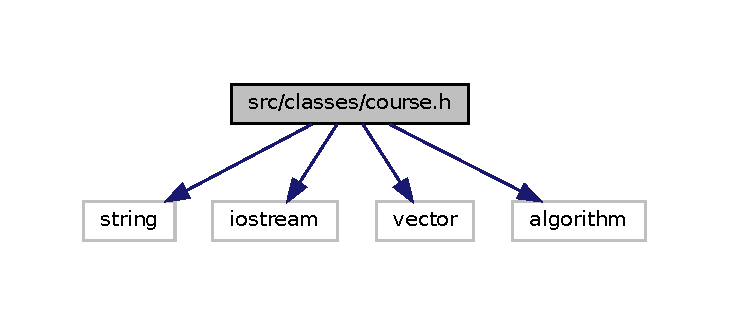
\includegraphics[width=350pt]{course_8h__incl}
\end{center}
\end{figure}
This graph shows which files directly or indirectly include this file\+:\nopagebreak
\begin{figure}[H]
\begin{center}
\leavevmode
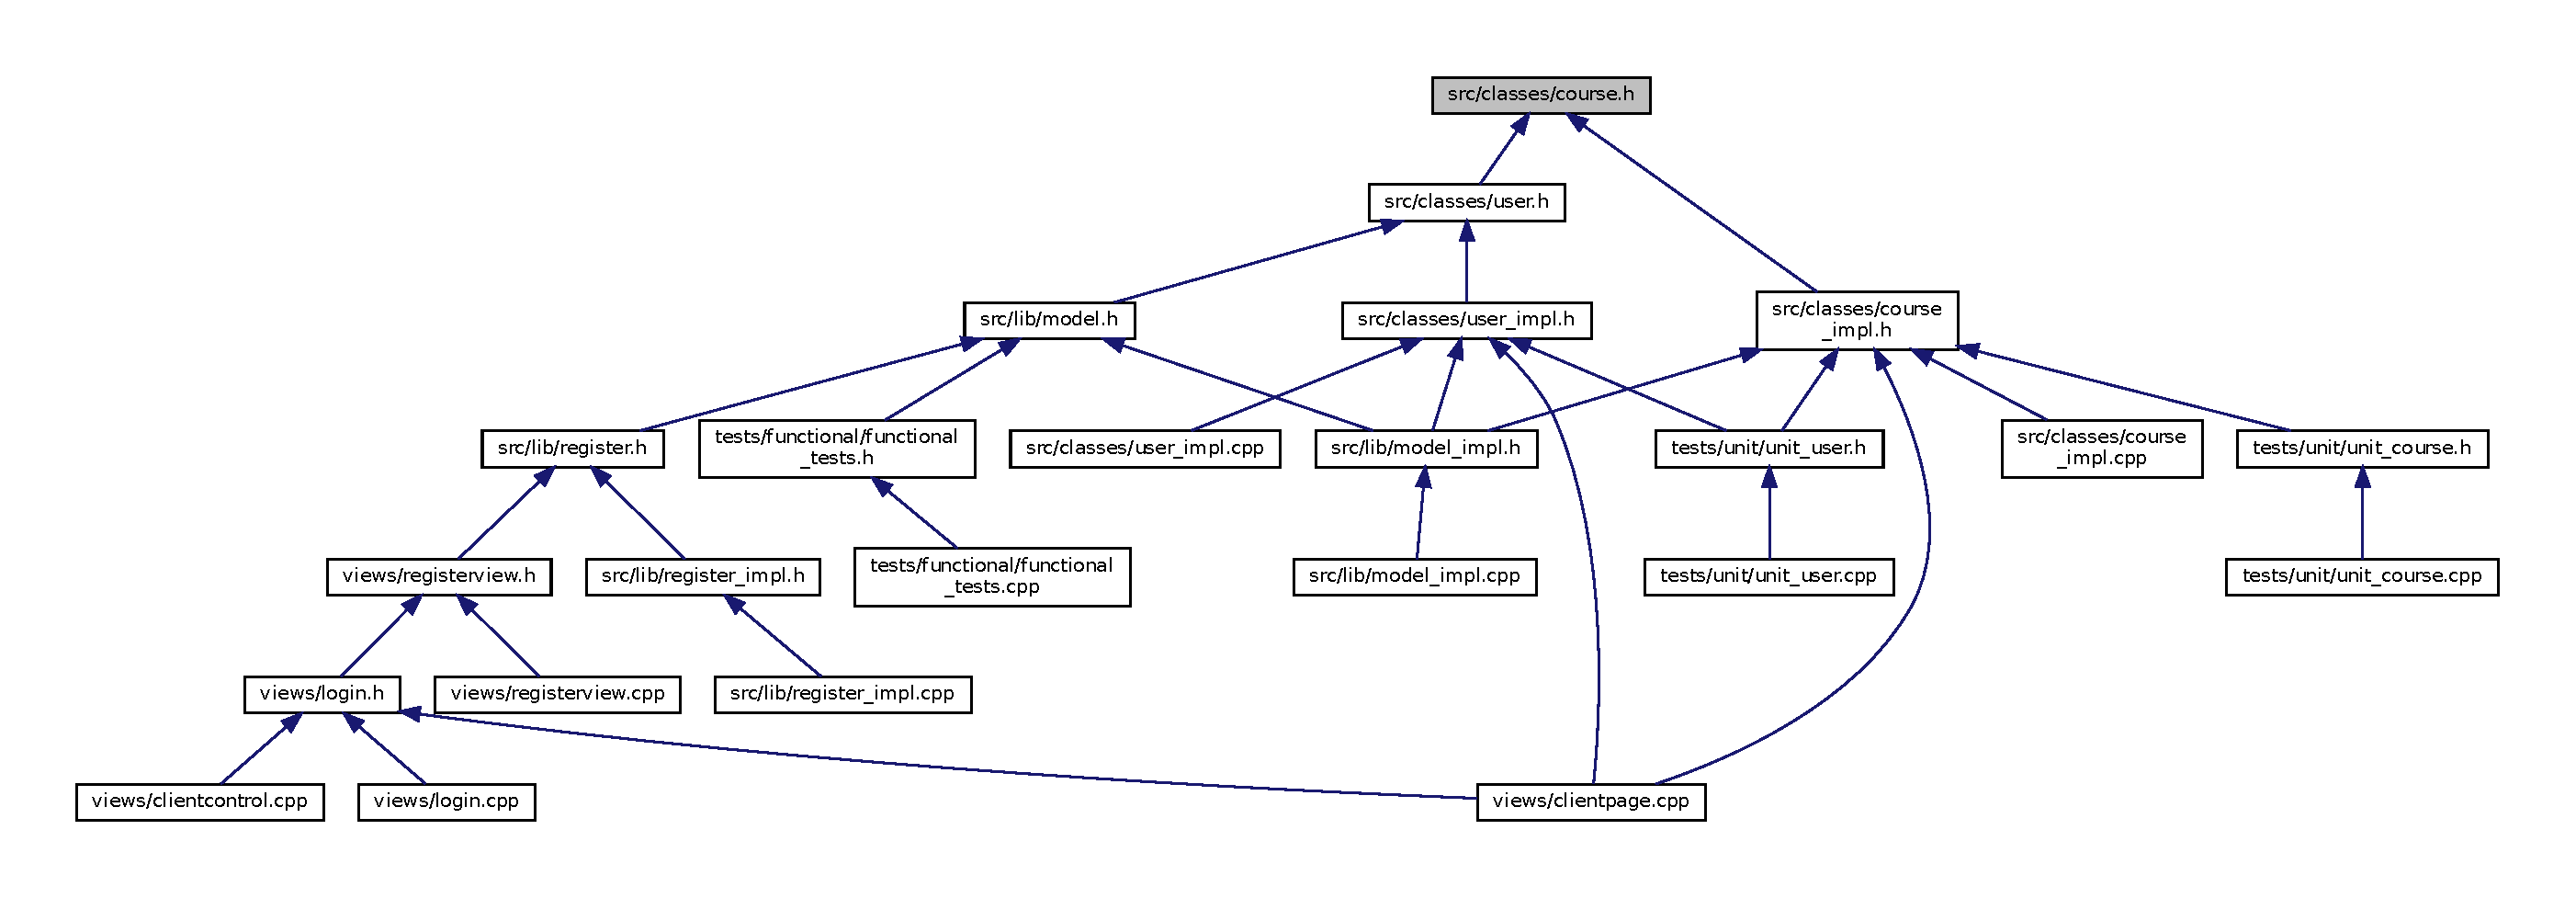
\includegraphics[width=350pt]{course_8h__dep__incl}
\end{center}
\end{figure}
\subsection*{Classes}
\begin{DoxyCompactItemize}
\item 
class \hyperlink{classCourse}{Course}
\begin{DoxyCompactList}\small\item\em this class represents a course \end{DoxyCompactList}\end{DoxyCompactItemize}

\hypertarget{course__impl_8cpp}{}\section{src/classes/course\+\_\+impl.cpp File Reference}
\label{course__impl_8cpp}\index{src/classes/course\+\_\+impl.\+cpp@{src/classes/course\+\_\+impl.\+cpp}}
{\ttfamily \#include \char`\"{}course\+\_\+impl.\+h\char`\"{}}\newline
Include dependency graph for course\+\_\+impl.\+cpp\+:
\nopagebreak
\begin{figure}[H]
\begin{center}
\leavevmode
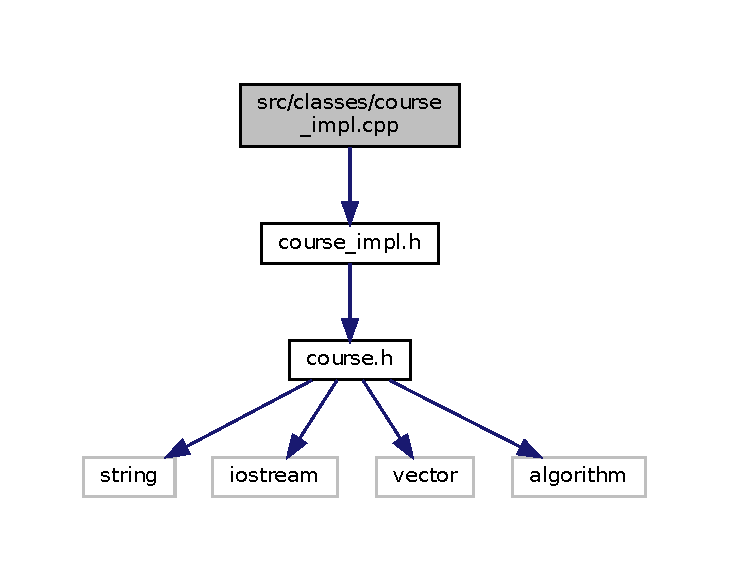
\includegraphics[width=350pt]{course__impl_8cpp__incl}
\end{center}
\end{figure}

\hypertarget{course__impl_8h}{}\section{src/classes/course\+\_\+impl.h File Reference}
\label{course__impl_8h}\index{src/classes/course\+\_\+impl.\+h@{src/classes/course\+\_\+impl.\+h}}
{\ttfamily \#include \char`\"{}course.\+h\char`\"{}}\newline
Include dependency graph for course\+\_\+impl.\+h\+:
\nopagebreak
\begin{figure}[H]
\begin{center}
\leavevmode
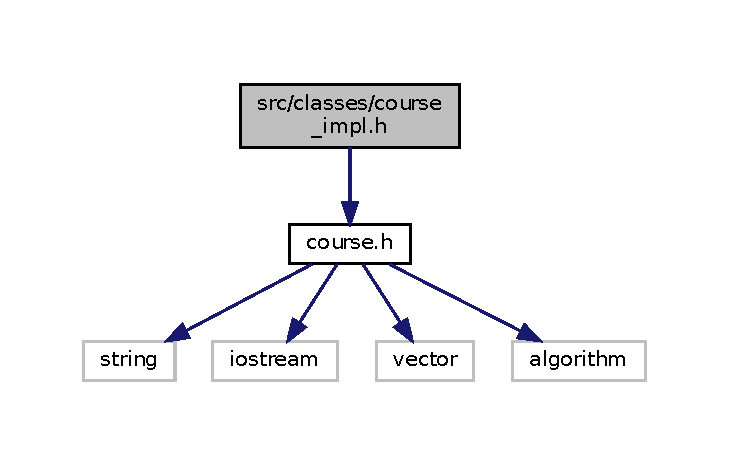
\includegraphics[width=350pt]{course__impl_8h__incl}
\end{center}
\end{figure}
This graph shows which files directly or indirectly include this file\+:
\nopagebreak
\begin{figure}[H]
\begin{center}
\leavevmode
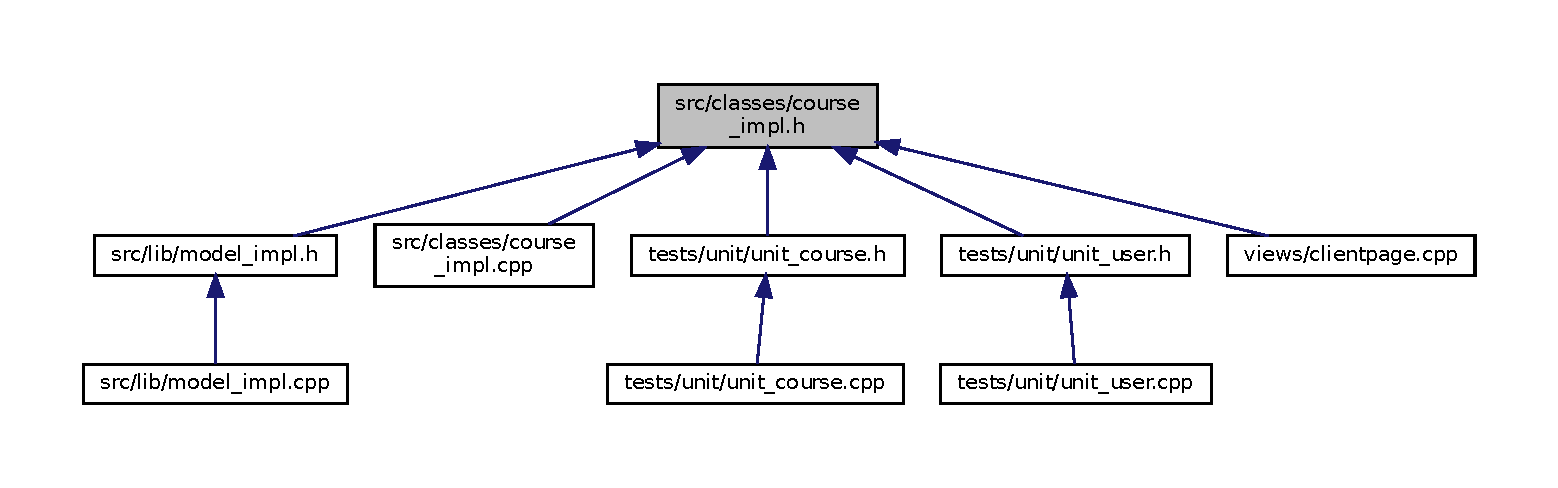
\includegraphics[width=350pt]{course__impl_8h__dep__incl}
\end{center}
\end{figure}
\subsection*{Classes}
\begin{DoxyCompactItemize}
\item 
class \hyperlink{classCourseImpl}{Course\+Impl}
\begin{DoxyCompactList}\small\item\em this represents a course \end{DoxyCompactList}\end{DoxyCompactItemize}

\hypertarget{user_8h}{}\section{src/classes/user.h File Reference}
\label{user_8h}\index{src/classes/user.\+h@{src/classes/user.\+h}}
{\ttfamily \#include \char`\"{}course.\+h\char`\"{}}\newline
{\ttfamily \#include $<$string$>$}\newline
{\ttfamily \#include $<$vector$>$}\newline
Include dependency graph for user.\+h\+:
\nopagebreak
\begin{figure}[H]
\begin{center}
\leavevmode
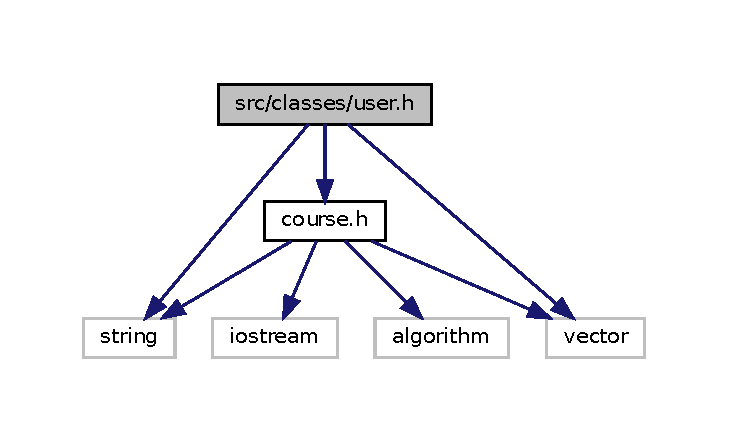
\includegraphics[width=350pt]{user_8h__incl}
\end{center}
\end{figure}
This graph shows which files directly or indirectly include this file\+:
\nopagebreak
\begin{figure}[H]
\begin{center}
\leavevmode
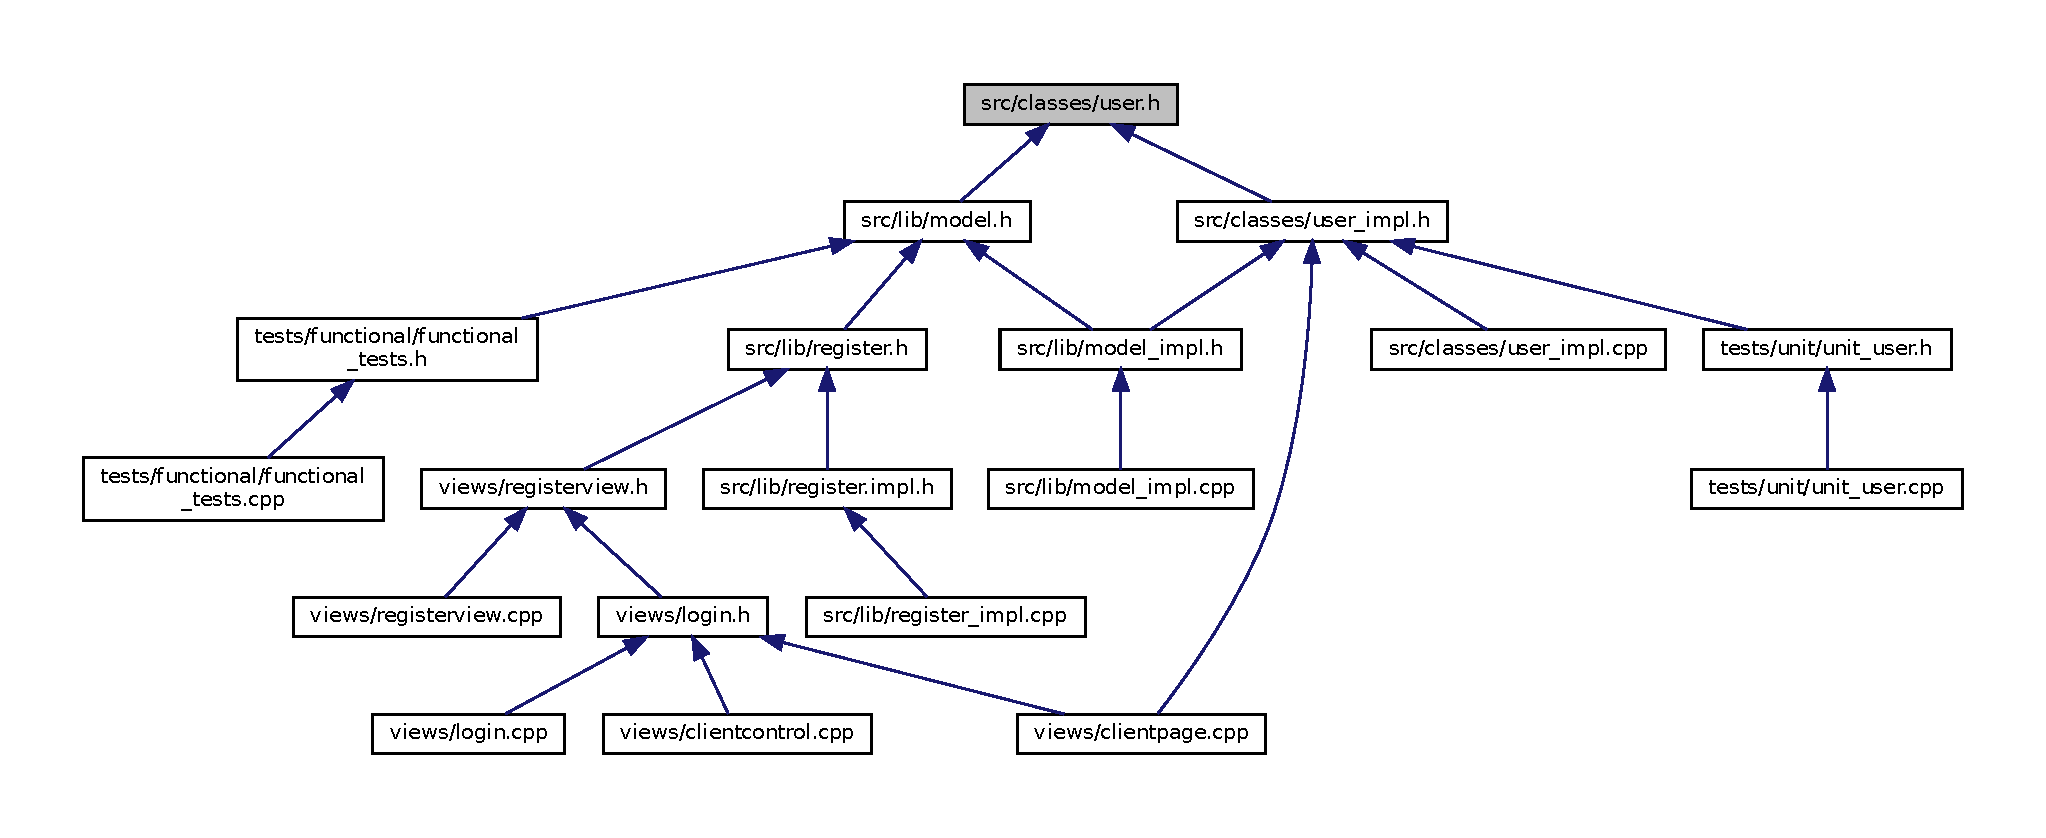
\includegraphics[width=350pt]{user_8h__dep__incl}
\end{center}
\end{figure}
\subsection*{Classes}
\begin{DoxyCompactItemize}
\item 
class \hyperlink{classUser}{User}
\begin{DoxyCompactList}\small\item\em this class represents an user \end{DoxyCompactList}\end{DoxyCompactItemize}

\hypertarget{user__impl_8cpp}{}\section{src/classes/user\+\_\+impl.cpp File Reference}
\label{user__impl_8cpp}\index{src/classes/user\+\_\+impl.\+cpp@{src/classes/user\+\_\+impl.\+cpp}}
{\ttfamily \#include \char`\"{}user\+\_\+impl.\+h\char`\"{}}\newline
Include dependency graph for user\+\_\+impl.\+cpp\+:
\nopagebreak
\begin{figure}[H]
\begin{center}
\leavevmode
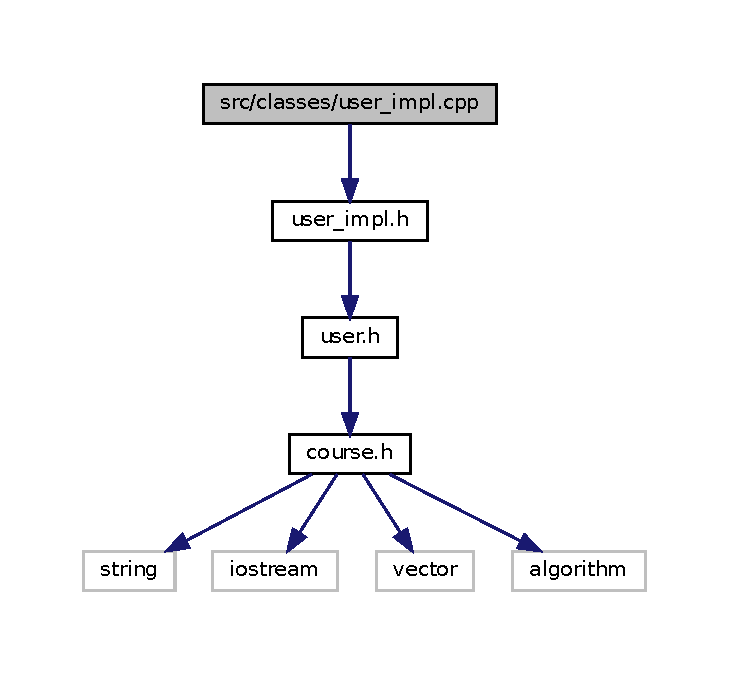
\includegraphics[width=350pt]{user__impl_8cpp__incl}
\end{center}
\end{figure}

\hypertarget{user__impl_8h}{}\section{src/classes/user\+\_\+impl.h File Reference}
\label{user__impl_8h}\index{src/classes/user\+\_\+impl.\+h@{src/classes/user\+\_\+impl.\+h}}
{\ttfamily \#include \char`\"{}user.\+h\char`\"{}}\newline
Include dependency graph for user\+\_\+impl.\+h\+:\nopagebreak
\begin{figure}[H]
\begin{center}
\leavevmode
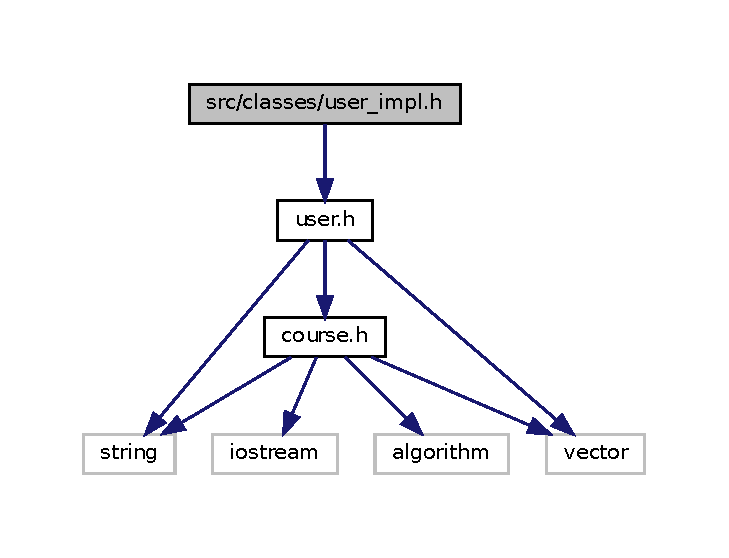
\includegraphics[width=350pt]{user__impl_8h__incl}
\end{center}
\end{figure}
This graph shows which files directly or indirectly include this file\+:\nopagebreak
\begin{figure}[H]
\begin{center}
\leavevmode
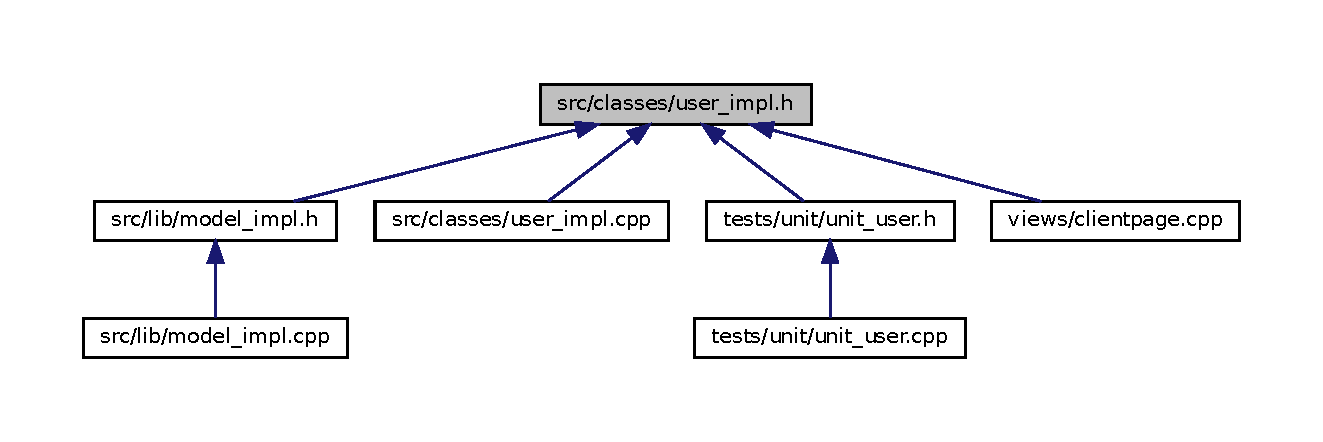
\includegraphics[width=350pt]{user__impl_8h__dep__incl}
\end{center}
\end{figure}
\subsection*{Classes}
\begin{DoxyCompactItemize}
\item 
class \hyperlink{classUserImpl}{User\+Impl}
\begin{DoxyCompactList}\small\item\em this class represents an user \end{DoxyCompactList}\end{DoxyCompactItemize}

\hypertarget{model_8h}{}\section{src/lib/model.h File Reference}
\label{model_8h}\index{src/lib/model.\+h@{src/lib/model.\+h}}
{\ttfamily \#include \char`\"{}../classes/course.\+h\char`\"{}}\newline
{\ttfamily \#include \char`\"{}../classes/user.\+h\char`\"{}}\newline
Include dependency graph for model.\+h\+:
\nopagebreak
\begin{figure}[H]
\begin{center}
\leavevmode
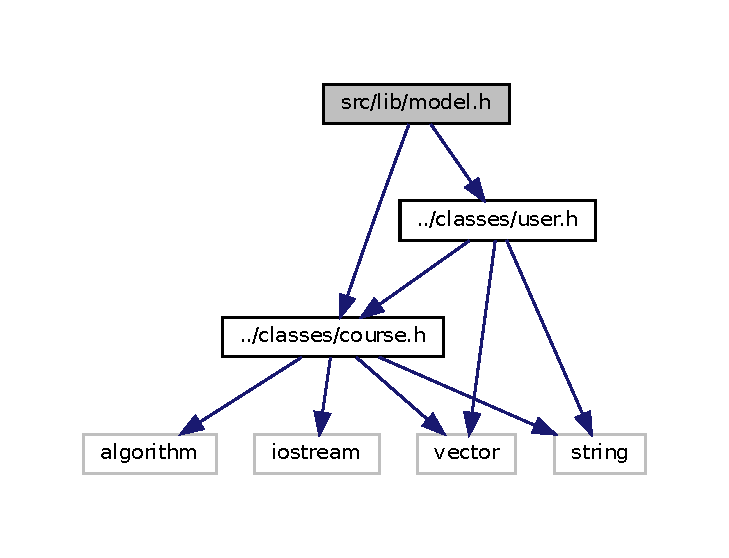
\includegraphics[width=350pt]{model_8h__incl}
\end{center}
\end{figure}
This graph shows which files directly or indirectly include this file\+:
\nopagebreak
\begin{figure}[H]
\begin{center}
\leavevmode
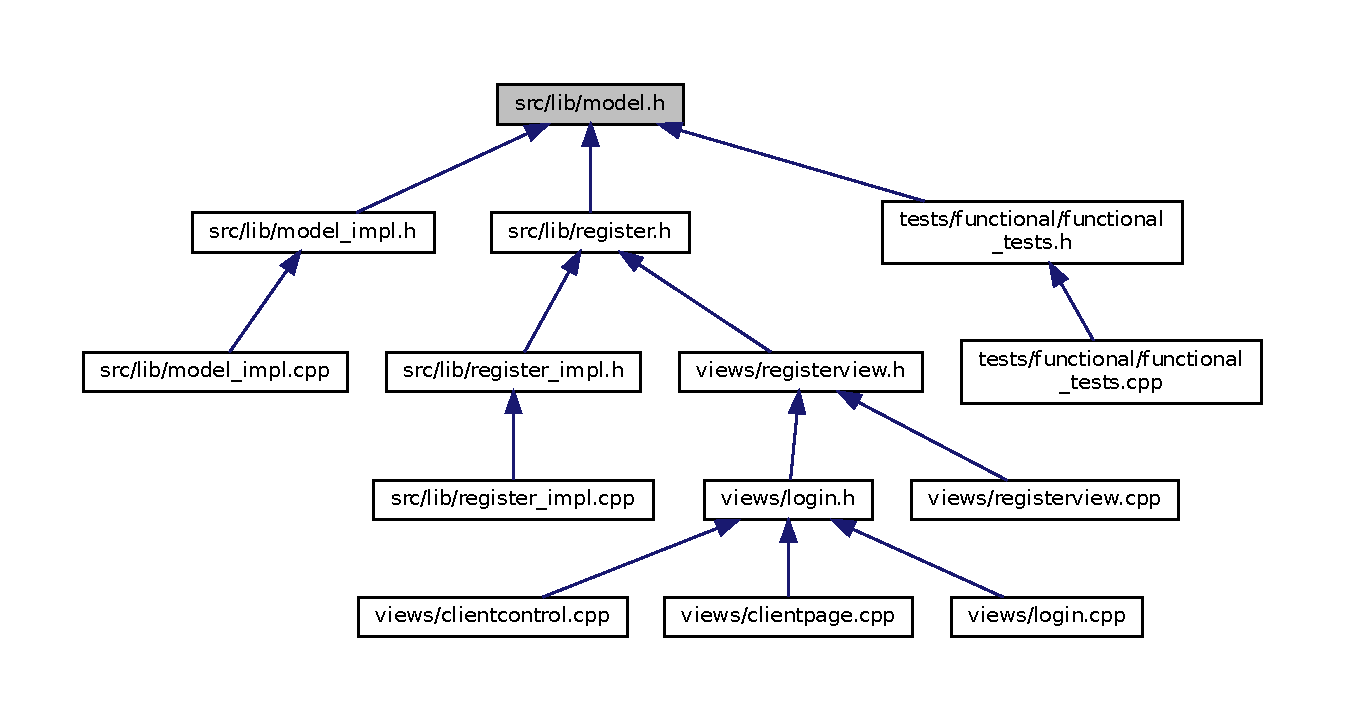
\includegraphics[width=350pt]{model_8h__dep__incl}
\end{center}
\end{figure}
\subsection*{Classes}
\begin{DoxyCompactItemize}
\item 
class \hyperlink{classModel}{Model}
\begin{DoxyCompactList}\small\item\em The \hyperlink{classModel}{Model} class. \end{DoxyCompactList}\end{DoxyCompactItemize}

\hypertarget{model__impl_8cpp}{}\section{src/lib/model\+\_\+impl.cpp File Reference}
\label{model__impl_8cpp}\index{src/lib/model\+\_\+impl.\+cpp@{src/lib/model\+\_\+impl.\+cpp}}
{\ttfamily \#include \char`\"{}model\+\_\+impl.\+h\char`\"{}}\newline
Include dependency graph for model\+\_\+impl.\+cpp\+:
\nopagebreak
\begin{figure}[H]
\begin{center}
\leavevmode
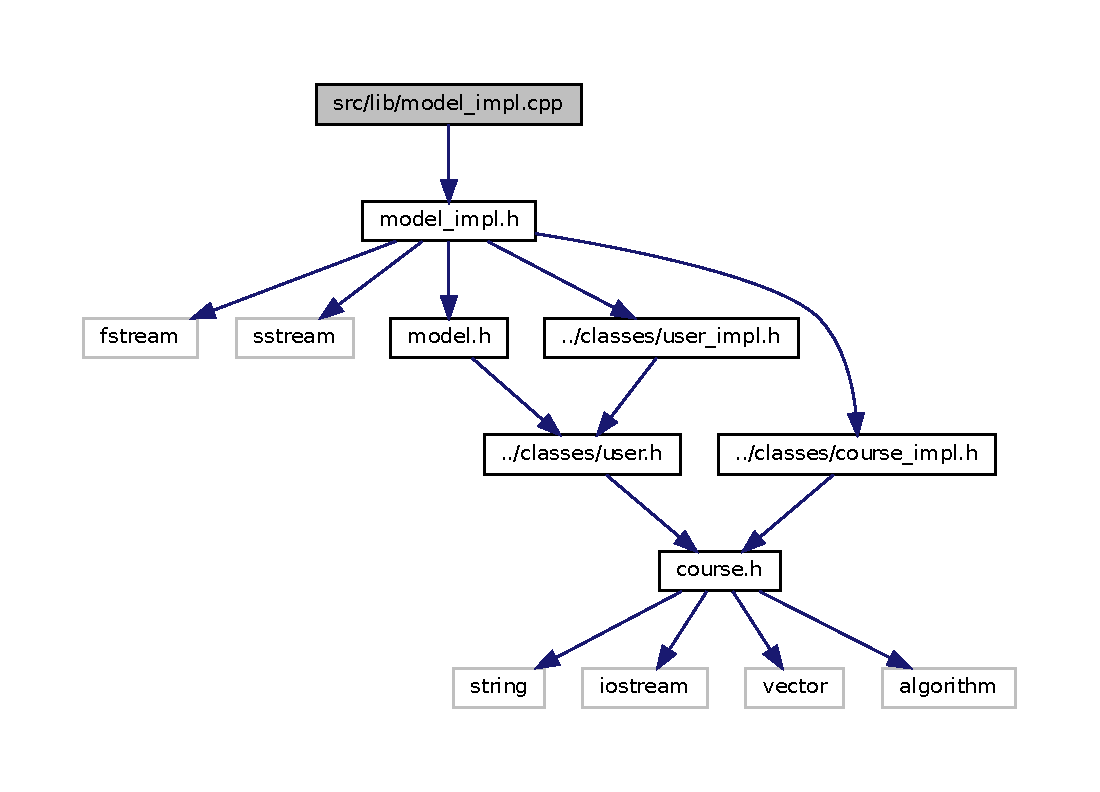
\includegraphics[width=350pt]{model__impl_8cpp__incl}
\end{center}
\end{figure}

\hypertarget{model__impl_8h}{}\section{src/lib/model\+\_\+impl.h File Reference}
\label{model__impl_8h}\index{src/lib/model\+\_\+impl.\+h@{src/lib/model\+\_\+impl.\+h}}
{\ttfamily \#include $<$fstream$>$}\newline
{\ttfamily \#include $<$sstream$>$}\newline
{\ttfamily \#include \char`\"{}model.\+h\char`\"{}}\newline
{\ttfamily \#include \char`\"{}../classes/course\+\_\+impl.\+h\char`\"{}}\newline
{\ttfamily \#include \char`\"{}../classes/user\+\_\+impl.\+h\char`\"{}}\newline
Include dependency graph for model\+\_\+impl.\+h\+:\nopagebreak
\begin{figure}[H]
\begin{center}
\leavevmode
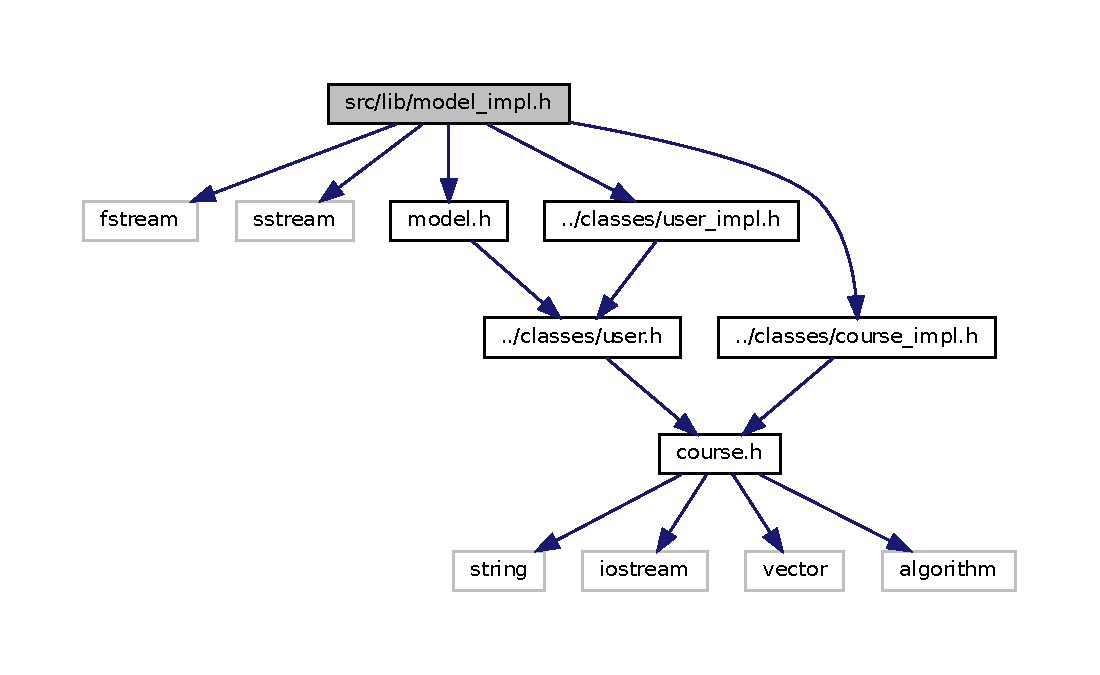
\includegraphics[width=350pt]{model__impl_8h__incl}
\end{center}
\end{figure}
This graph shows which files directly or indirectly include this file\+:\nopagebreak
\begin{figure}[H]
\begin{center}
\leavevmode
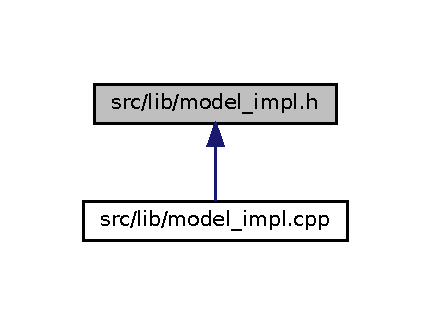
\includegraphics[width=207pt]{model__impl_8h__dep__incl}
\end{center}
\end{figure}
\subsection*{Classes}
\begin{DoxyCompactItemize}
\item 
class \hyperlink{classModelImpl}{Model\+Impl}
\begin{DoxyCompactList}\small\item\em Derived class where all methods will be implemented according to the desired modeling. \end{DoxyCompactList}\end{DoxyCompactItemize}

\hypertarget{register_8h}{}\section{src/lib/register.h File Reference}
\label{register_8h}\index{src/lib/register.\+h@{src/lib/register.\+h}}
{\ttfamily \#include \char`\"{}model.\+h\char`\"{}}\newline
{\ttfamily \#include $<$Q\+Message\+Box$>$}\newline
Include dependency graph for register.\+h\+:
\nopagebreak
\begin{figure}[H]
\begin{center}
\leavevmode
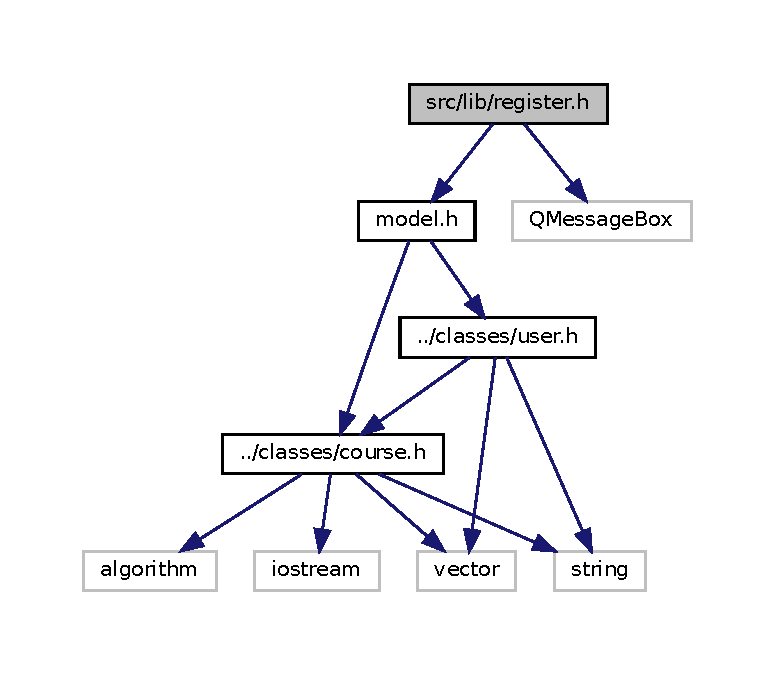
\includegraphics[width=350pt]{register_8h__incl}
\end{center}
\end{figure}
This graph shows which files directly or indirectly include this file\+:
\nopagebreak
\begin{figure}[H]
\begin{center}
\leavevmode
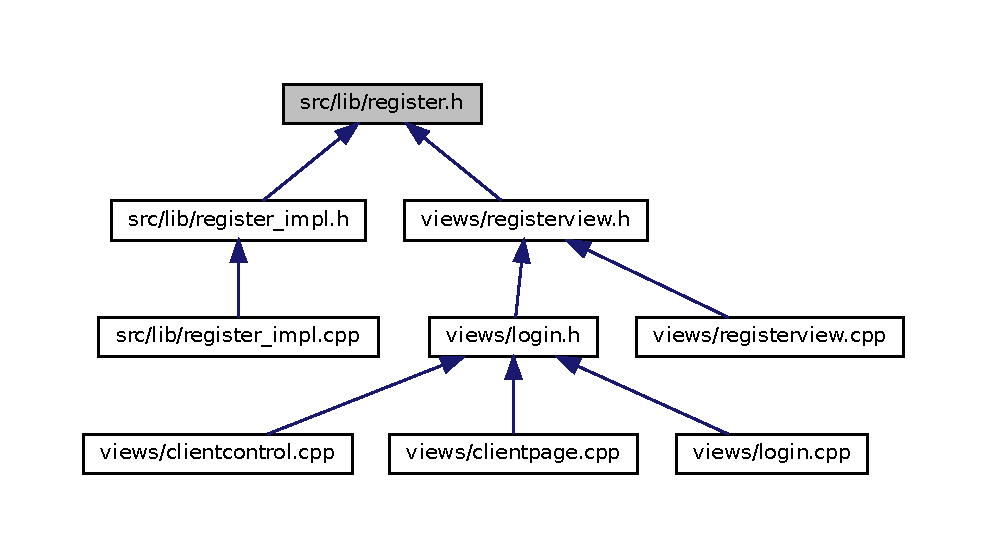
\includegraphics[width=350pt]{register_8h__dep__incl}
\end{center}
\end{figure}
\subsection*{Classes}
\begin{DoxyCompactItemize}
\item 
class \hyperlink{classRegister}{Register}
\begin{DoxyCompactList}\small\item\em this class represents a register \end{DoxyCompactList}\end{DoxyCompactItemize}

\hypertarget{register__impl_8cpp}{}\section{src/lib/register\+\_\+impl.cpp File Reference}
\label{register__impl_8cpp}\index{src/lib/register\+\_\+impl.\+cpp@{src/lib/register\+\_\+impl.\+cpp}}
{\ttfamily \#include \char`\"{}register.\+impl.\+h\char`\"{}}\newline
{\ttfamily \#include \char`\"{}ui\+\_\+registerview.\+h\char`\"{}}\newline
{\ttfamily \#include $<$Q\+H\+Box\+Layout$>$}\newline
{\ttfamily \#include $<$iostream$>$}\newline
Include dependency graph for register\+\_\+impl.\+cpp\+:
\nopagebreak
\begin{figure}[H]
\begin{center}
\leavevmode
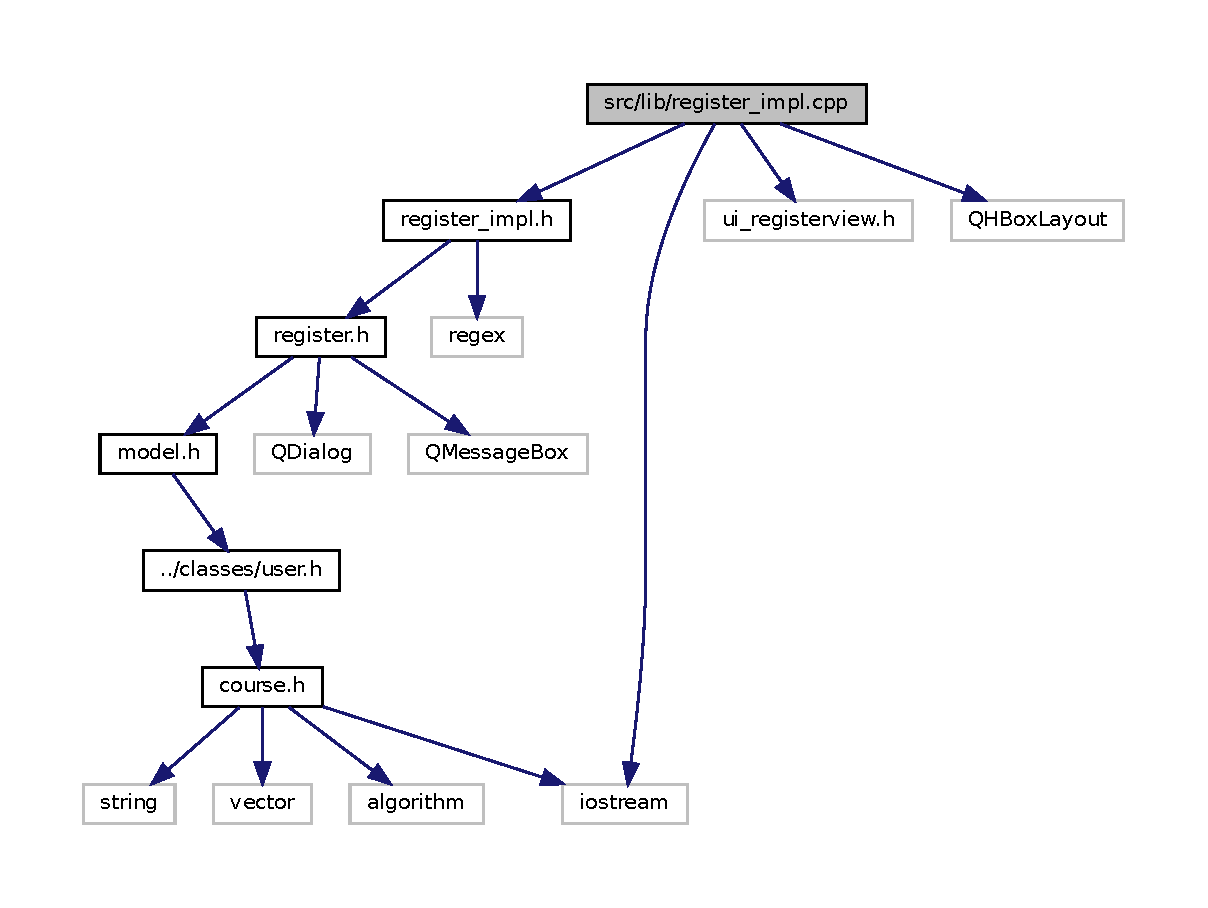
\includegraphics[width=350pt]{register__impl_8cpp__incl}
\end{center}
\end{figure}

\hypertarget{register__impl_8h}{}\section{src/lib/register\+\_\+impl.h File Reference}
\label{register__impl_8h}\index{src/lib/register\+\_\+impl.\+h@{src/lib/register\+\_\+impl.\+h}}
{\ttfamily \#include \char`\"{}register.\+h\char`\"{}}\newline
{\ttfamily \#include $<$regex$>$}\newline
Include dependency graph for register\+\_\+impl.\+h\+:
\nopagebreak
\begin{figure}[H]
\begin{center}
\leavevmode
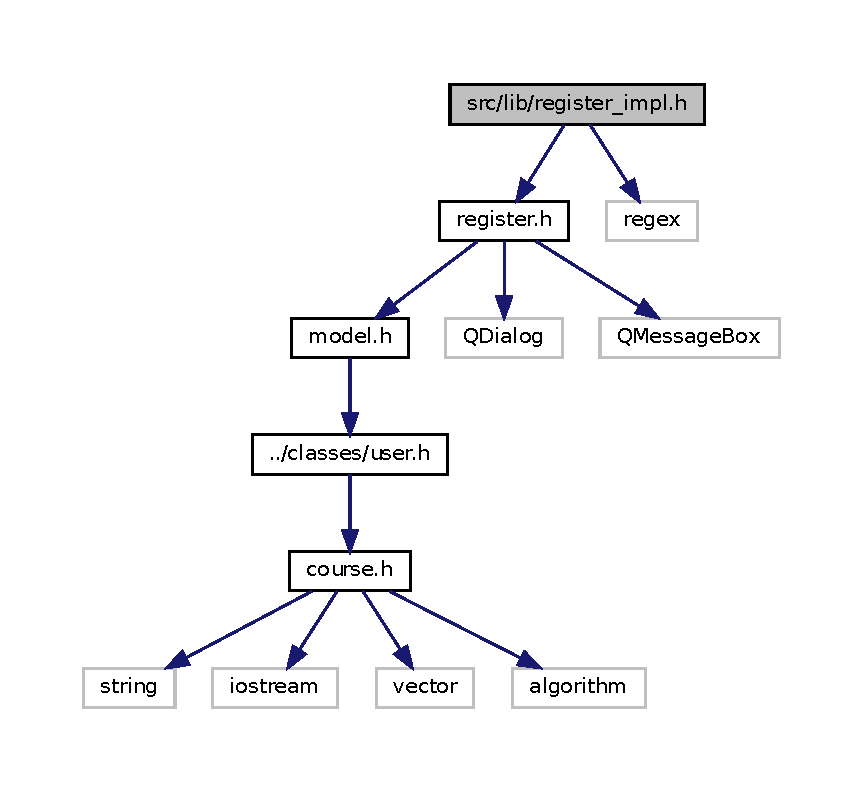
\includegraphics[width=350pt]{register__impl_8h__incl}
\end{center}
\end{figure}
This graph shows which files directly or indirectly include this file\+:
\nopagebreak
\begin{figure}[H]
\begin{center}
\leavevmode
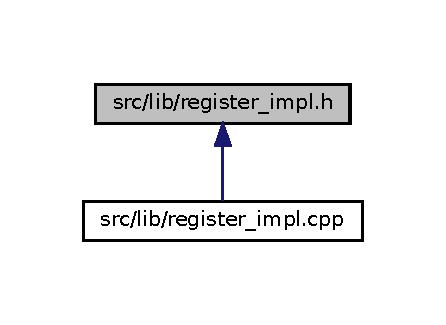
\includegraphics[width=214pt]{register__impl_8h__dep__incl}
\end{center}
\end{figure}
\subsection*{Classes}
\begin{DoxyCompactItemize}
\item 
class \hyperlink{classRegisterImpl}{Register\+Impl}
\begin{DoxyCompactList}\small\item\em this class represents a register \end{DoxyCompactList}\end{DoxyCompactItemize}

\hypertarget{functional__tests_8cpp}{}\section{tests/functional/functional\+\_\+tests.cpp File Reference}
\label{functional__tests_8cpp}\index{tests/functional/functional\+\_\+tests.\+cpp@{tests/functional/functional\+\_\+tests.\+cpp}}
{\ttfamily \#include \char`\"{}functional\+\_\+tests.\+h\char`\"{}}\newline
Include dependency graph for functional\+\_\+tests.\+cpp\+:\nopagebreak
\begin{figure}[H]
\begin{center}
\leavevmode
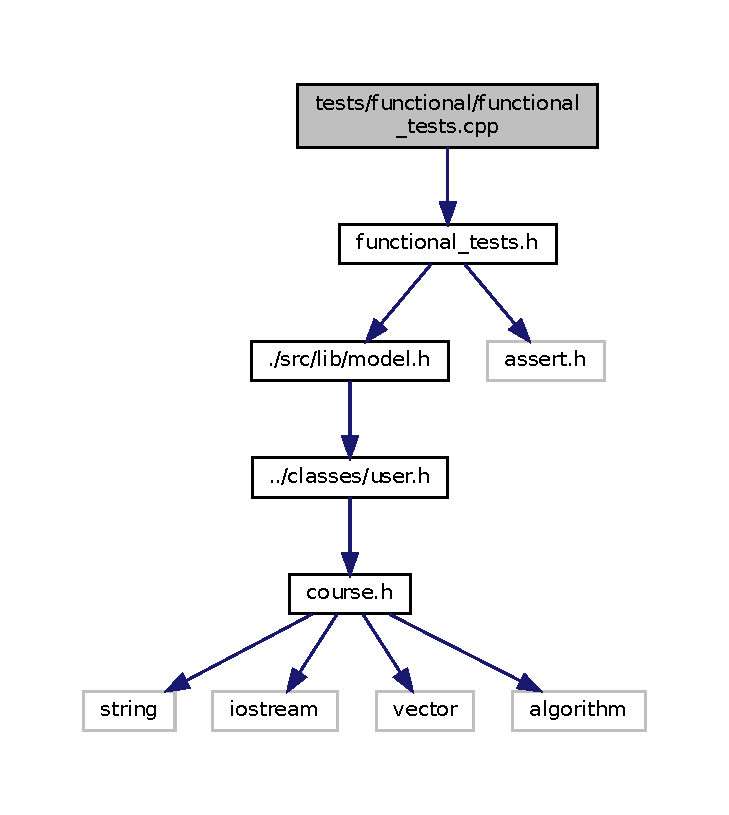
\includegraphics[width=350pt]{functional__tests_8cpp__incl}
\end{center}
\end{figure}
\subsection*{Functions}
\begin{DoxyCompactItemize}
\item 
void \hyperlink{functional__tests_8cpp_ac66c0c95899deebf8facb8a3b93eb06e}{functional\+\_\+tests} ()
\begin{DoxyCompactList}\small\item\em Tests functional. \end{DoxyCompactList}\end{DoxyCompactItemize}


\subsection{Function Documentation}
\mbox{\Hypertarget{functional__tests_8cpp_ac66c0c95899deebf8facb8a3b93eb06e}\label{functional__tests_8cpp_ac66c0c95899deebf8facb8a3b93eb06e}} 
\index{functional\+\_\+tests.\+cpp@{functional\+\_\+tests.\+cpp}!functional\+\_\+tests@{functional\+\_\+tests}}
\index{functional\+\_\+tests@{functional\+\_\+tests}!functional\+\_\+tests.\+cpp@{functional\+\_\+tests.\+cpp}}
\subsubsection{\texorpdfstring{functional\+\_\+tests()}{functional\_tests()}}
{\footnotesize\ttfamily void functional\+\_\+tests (\begin{DoxyParamCaption}{ }\end{DoxyParamCaption})}



Tests functional. 


\hypertarget{functional__tests_8h}{}\section{tests/functional/functional\+\_\+tests.h File Reference}
\label{functional__tests_8h}\index{tests/functional/functional\+\_\+tests.\+h@{tests/functional/functional\+\_\+tests.\+h}}
{\ttfamily \#include \char`\"{}./src/lib/model.\+h\char`\"{}}\newline
{\ttfamily \#include $<$assert.\+h$>$}\newline
Include dependency graph for functional\+\_\+tests.\+h\+:\nopagebreak
\begin{figure}[H]
\begin{center}
\leavevmode
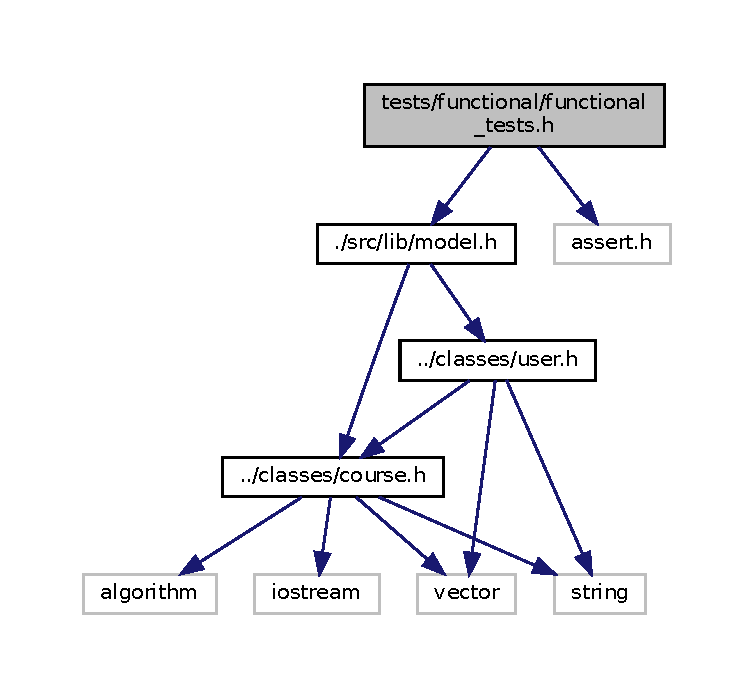
\includegraphics[width=350pt]{functional__tests_8h__incl}
\end{center}
\end{figure}
This graph shows which files directly or indirectly include this file\+:\nopagebreak
\begin{figure}[H]
\begin{center}
\leavevmode
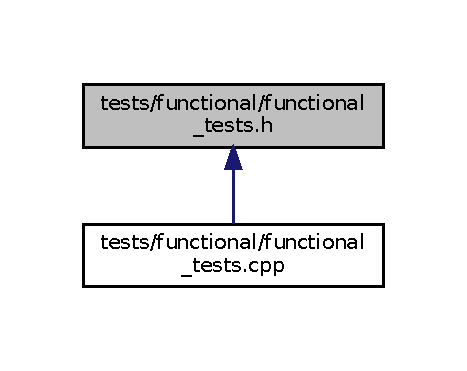
\includegraphics[width=224pt]{functional__tests_8h__dep__incl}
\end{center}
\end{figure}
\subsection*{Functions}
\begin{DoxyCompactItemize}
\item 
void \hyperlink{functional__tests_8h_ac66c0c95899deebf8facb8a3b93eb06e}{functional\+\_\+tests} ()
\begin{DoxyCompactList}\small\item\em Tests functional. \end{DoxyCompactList}\end{DoxyCompactItemize}


\subsection{Function Documentation}
\mbox{\Hypertarget{functional__tests_8h_ac66c0c95899deebf8facb8a3b93eb06e}\label{functional__tests_8h_ac66c0c95899deebf8facb8a3b93eb06e}} 
\index{functional\+\_\+tests.\+h@{functional\+\_\+tests.\+h}!functional\+\_\+tests@{functional\+\_\+tests}}
\index{functional\+\_\+tests@{functional\+\_\+tests}!functional\+\_\+tests.\+h@{functional\+\_\+tests.\+h}}
\subsubsection{\texorpdfstring{functional\+\_\+tests()}{functional\_tests()}}
{\footnotesize\ttfamily void functional\+\_\+tests (\begin{DoxyParamCaption}{ }\end{DoxyParamCaption})}



Tests functional. 


\hypertarget{unit__course_8cpp}{}\section{tests/unit/unit\+\_\+course.cpp File Reference}
\label{unit__course_8cpp}\index{tests/unit/unit\+\_\+course.\+cpp@{tests/unit/unit\+\_\+course.\+cpp}}
{\ttfamily \#include \char`\"{}unit\+\_\+course.\+h\char`\"{}}\newline
{\ttfamily \#include $<$iostream$>$}\newline
Include dependency graph for unit\+\_\+course.\+cpp\+:
\nopagebreak
\begin{figure}[H]
\begin{center}
\leavevmode
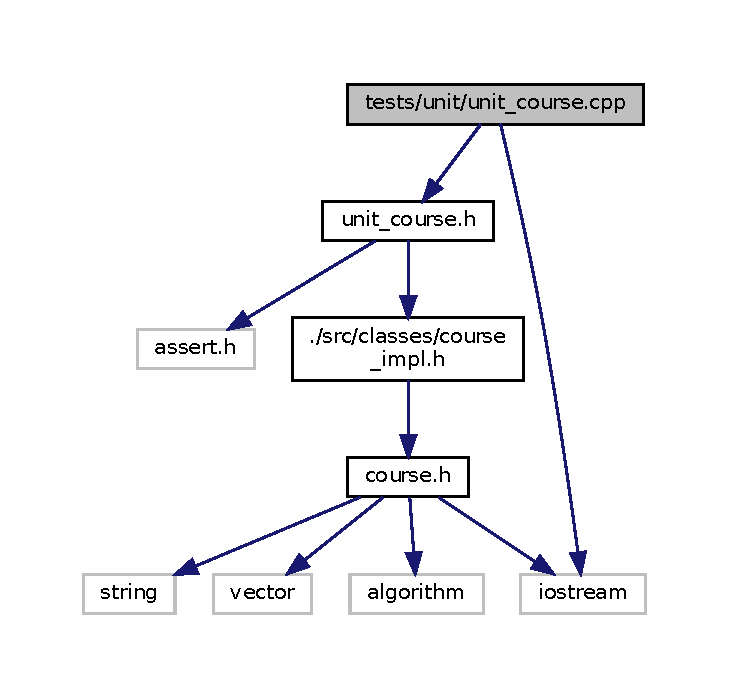
\includegraphics[width=350pt]{unit__course_8cpp__incl}
\end{center}
\end{figure}
\subsection*{Functions}
\begin{DoxyCompactItemize}
\item 
void \hyperlink{unit__course_8cpp_adec5bf19c872e2ae9f750d802fe574aa}{unit\+\_\+course\+\_\+constructor} ()
\begin{DoxyCompactList}\small\item\em Tests class constructors. \end{DoxyCompactList}\item 
void \hyperlink{unit__course_8cpp_a8c65b7fbb1fedbd6814bebfd04fbaa9c}{unit\+\_\+course\+\_\+destructor} ()
\begin{DoxyCompactList}\small\item\em Tests class destructors. \end{DoxyCompactList}\item 
void \hyperlink{unit__course_8cpp_acabdbc2225ea8a478abb2fca14755953}{unit\+\_\+course\+\_\+get\+Name} ()
\begin{DoxyCompactList}\small\item\em Tests get\+Name method. \end{DoxyCompactList}\item 
void \hyperlink{unit__course_8cpp_a8dd3f90e5ec3eb47f3b3a638c485f8ac}{unit\+\_\+course\+\_\+set\+Name} ()
\begin{DoxyCompactList}\small\item\em Tests set\+Name method. \end{DoxyCompactList}\item 
void \hyperlink{unit__course_8cpp_a41ae3d30fb03b6d50d422090f070ef66}{unit\+\_\+course\+\_\+get\+Description} ()
\begin{DoxyCompactList}\small\item\em Tests get\+Description method. \end{DoxyCompactList}\item 
void \hyperlink{unit__course_8cpp_a0cc66fb03dd51e8ccae1abe65c921a2e}{unit\+\_\+course\+\_\+set\+Description} ()
\begin{DoxyCompactList}\small\item\em Tests set\+Description method. \end{DoxyCompactList}\item 
void \hyperlink{unit__course_8cpp_a66cb19343268715b0b9ff66d6e1da205}{unit\+\_\+course\+\_\+get\+Price} ()
\begin{DoxyCompactList}\small\item\em Tests get\+Price method. \end{DoxyCompactList}\item 
void \hyperlink{unit__course_8cpp_a6cca31a484b282f2c55932516207867a}{unit\+\_\+course\+\_\+set\+Price} ()
\begin{DoxyCompactList}\small\item\em Tests set\+Price method. \end{DoxyCompactList}\item 
void \hyperlink{unit__course_8cpp_a72d485245f31ea71af771f0b1ff90aca}{unit\+\_\+course\+\_\+assignment} ()
\begin{DoxyCompactList}\small\item\em Tests the assignment operator overload. \end{DoxyCompactList}\item 
void \hyperlink{unit__course_8cpp_ac1cac74acf8a743480369a340ddd4383}{run\+\_\+unit\+\_\+tests\+\_\+course} ()
\begin{DoxyCompactList}\small\item\em Runs all unit tests of the \hyperlink{classCourse}{Course} class. \end{DoxyCompactList}\end{DoxyCompactItemize}


\subsection{Function Documentation}
\mbox{\Hypertarget{unit__course_8cpp_ac1cac74acf8a743480369a340ddd4383}\label{unit__course_8cpp_ac1cac74acf8a743480369a340ddd4383}} 
\index{unit\+\_\+course.\+cpp@{unit\+\_\+course.\+cpp}!run\+\_\+unit\+\_\+tests\+\_\+course@{run\+\_\+unit\+\_\+tests\+\_\+course}}
\index{run\+\_\+unit\+\_\+tests\+\_\+course@{run\+\_\+unit\+\_\+tests\+\_\+course}!unit\+\_\+course.\+cpp@{unit\+\_\+course.\+cpp}}
\subsubsection{\texorpdfstring{run\+\_\+unit\+\_\+tests\+\_\+course()}{run\_unit\_tests\_course()}}
{\footnotesize\ttfamily void run\+\_\+unit\+\_\+tests\+\_\+course (\begin{DoxyParamCaption}{ }\end{DoxyParamCaption})}



Runs all unit tests of the \hyperlink{classCourse}{Course} class. 

\mbox{\Hypertarget{unit__course_8cpp_a72d485245f31ea71af771f0b1ff90aca}\label{unit__course_8cpp_a72d485245f31ea71af771f0b1ff90aca}} 
\index{unit\+\_\+course.\+cpp@{unit\+\_\+course.\+cpp}!unit\+\_\+course\+\_\+assignment@{unit\+\_\+course\+\_\+assignment}}
\index{unit\+\_\+course\+\_\+assignment@{unit\+\_\+course\+\_\+assignment}!unit\+\_\+course.\+cpp@{unit\+\_\+course.\+cpp}}
\subsubsection{\texorpdfstring{unit\+\_\+course\+\_\+assignment()}{unit\_course\_assignment()}}
{\footnotesize\ttfamily void unit\+\_\+course\+\_\+assignment (\begin{DoxyParamCaption}{ }\end{DoxyParamCaption})}



Tests the assignment operator overload. 

\mbox{\Hypertarget{unit__course_8cpp_adec5bf19c872e2ae9f750d802fe574aa}\label{unit__course_8cpp_adec5bf19c872e2ae9f750d802fe574aa}} 
\index{unit\+\_\+course.\+cpp@{unit\+\_\+course.\+cpp}!unit\+\_\+course\+\_\+constructor@{unit\+\_\+course\+\_\+constructor}}
\index{unit\+\_\+course\+\_\+constructor@{unit\+\_\+course\+\_\+constructor}!unit\+\_\+course.\+cpp@{unit\+\_\+course.\+cpp}}
\subsubsection{\texorpdfstring{unit\+\_\+course\+\_\+constructor()}{unit\_course\_constructor()}}
{\footnotesize\ttfamily void unit\+\_\+course\+\_\+constructor (\begin{DoxyParamCaption}{ }\end{DoxyParamCaption})}



Tests class constructors. 

\mbox{\Hypertarget{unit__course_8cpp_a8c65b7fbb1fedbd6814bebfd04fbaa9c}\label{unit__course_8cpp_a8c65b7fbb1fedbd6814bebfd04fbaa9c}} 
\index{unit\+\_\+course.\+cpp@{unit\+\_\+course.\+cpp}!unit\+\_\+course\+\_\+destructor@{unit\+\_\+course\+\_\+destructor}}
\index{unit\+\_\+course\+\_\+destructor@{unit\+\_\+course\+\_\+destructor}!unit\+\_\+course.\+cpp@{unit\+\_\+course.\+cpp}}
\subsubsection{\texorpdfstring{unit\+\_\+course\+\_\+destructor()}{unit\_course\_destructor()}}
{\footnotesize\ttfamily void unit\+\_\+course\+\_\+destructor (\begin{DoxyParamCaption}{ }\end{DoxyParamCaption})}



Tests class destructors. 

\mbox{\Hypertarget{unit__course_8cpp_a41ae3d30fb03b6d50d422090f070ef66}\label{unit__course_8cpp_a41ae3d30fb03b6d50d422090f070ef66}} 
\index{unit\+\_\+course.\+cpp@{unit\+\_\+course.\+cpp}!unit\+\_\+course\+\_\+get\+Description@{unit\+\_\+course\+\_\+get\+Description}}
\index{unit\+\_\+course\+\_\+get\+Description@{unit\+\_\+course\+\_\+get\+Description}!unit\+\_\+course.\+cpp@{unit\+\_\+course.\+cpp}}
\subsubsection{\texorpdfstring{unit\+\_\+course\+\_\+get\+Description()}{unit\_course\_getDescription()}}
{\footnotesize\ttfamily void unit\+\_\+course\+\_\+get\+Description (\begin{DoxyParamCaption}{ }\end{DoxyParamCaption})}



Tests get\+Description method. 

\mbox{\Hypertarget{unit__course_8cpp_acabdbc2225ea8a478abb2fca14755953}\label{unit__course_8cpp_acabdbc2225ea8a478abb2fca14755953}} 
\index{unit\+\_\+course.\+cpp@{unit\+\_\+course.\+cpp}!unit\+\_\+course\+\_\+get\+Name@{unit\+\_\+course\+\_\+get\+Name}}
\index{unit\+\_\+course\+\_\+get\+Name@{unit\+\_\+course\+\_\+get\+Name}!unit\+\_\+course.\+cpp@{unit\+\_\+course.\+cpp}}
\subsubsection{\texorpdfstring{unit\+\_\+course\+\_\+get\+Name()}{unit\_course\_getName()}}
{\footnotesize\ttfamily void unit\+\_\+course\+\_\+get\+Name (\begin{DoxyParamCaption}{ }\end{DoxyParamCaption})}



Tests get\+Name method. 

\mbox{\Hypertarget{unit__course_8cpp_a66cb19343268715b0b9ff66d6e1da205}\label{unit__course_8cpp_a66cb19343268715b0b9ff66d6e1da205}} 
\index{unit\+\_\+course.\+cpp@{unit\+\_\+course.\+cpp}!unit\+\_\+course\+\_\+get\+Price@{unit\+\_\+course\+\_\+get\+Price}}
\index{unit\+\_\+course\+\_\+get\+Price@{unit\+\_\+course\+\_\+get\+Price}!unit\+\_\+course.\+cpp@{unit\+\_\+course.\+cpp}}
\subsubsection{\texorpdfstring{unit\+\_\+course\+\_\+get\+Price()}{unit\_course\_getPrice()}}
{\footnotesize\ttfamily void unit\+\_\+course\+\_\+get\+Price (\begin{DoxyParamCaption}{ }\end{DoxyParamCaption})}



Tests get\+Price method. 

\mbox{\Hypertarget{unit__course_8cpp_a0cc66fb03dd51e8ccae1abe65c921a2e}\label{unit__course_8cpp_a0cc66fb03dd51e8ccae1abe65c921a2e}} 
\index{unit\+\_\+course.\+cpp@{unit\+\_\+course.\+cpp}!unit\+\_\+course\+\_\+set\+Description@{unit\+\_\+course\+\_\+set\+Description}}
\index{unit\+\_\+course\+\_\+set\+Description@{unit\+\_\+course\+\_\+set\+Description}!unit\+\_\+course.\+cpp@{unit\+\_\+course.\+cpp}}
\subsubsection{\texorpdfstring{unit\+\_\+course\+\_\+set\+Description()}{unit\_course\_setDescription()}}
{\footnotesize\ttfamily void unit\+\_\+course\+\_\+set\+Description (\begin{DoxyParamCaption}{ }\end{DoxyParamCaption})}



Tests set\+Description method. 

\mbox{\Hypertarget{unit__course_8cpp_a8dd3f90e5ec3eb47f3b3a638c485f8ac}\label{unit__course_8cpp_a8dd3f90e5ec3eb47f3b3a638c485f8ac}} 
\index{unit\+\_\+course.\+cpp@{unit\+\_\+course.\+cpp}!unit\+\_\+course\+\_\+set\+Name@{unit\+\_\+course\+\_\+set\+Name}}
\index{unit\+\_\+course\+\_\+set\+Name@{unit\+\_\+course\+\_\+set\+Name}!unit\+\_\+course.\+cpp@{unit\+\_\+course.\+cpp}}
\subsubsection{\texorpdfstring{unit\+\_\+course\+\_\+set\+Name()}{unit\_course\_setName()}}
{\footnotesize\ttfamily void unit\+\_\+course\+\_\+set\+Name (\begin{DoxyParamCaption}{ }\end{DoxyParamCaption})}



Tests set\+Name method. 

\mbox{\Hypertarget{unit__course_8cpp_a6cca31a484b282f2c55932516207867a}\label{unit__course_8cpp_a6cca31a484b282f2c55932516207867a}} 
\index{unit\+\_\+course.\+cpp@{unit\+\_\+course.\+cpp}!unit\+\_\+course\+\_\+set\+Price@{unit\+\_\+course\+\_\+set\+Price}}
\index{unit\+\_\+course\+\_\+set\+Price@{unit\+\_\+course\+\_\+set\+Price}!unit\+\_\+course.\+cpp@{unit\+\_\+course.\+cpp}}
\subsubsection{\texorpdfstring{unit\+\_\+course\+\_\+set\+Price()}{unit\_course\_setPrice()}}
{\footnotesize\ttfamily void unit\+\_\+course\+\_\+set\+Price (\begin{DoxyParamCaption}{ }\end{DoxyParamCaption})}



Tests set\+Price method. 


\hypertarget{unit__course_8h}{}\section{tests/unit/unit\+\_\+course.h File Reference}
\label{unit__course_8h}\index{tests/unit/unit\+\_\+course.\+h@{tests/unit/unit\+\_\+course.\+h}}
{\ttfamily \#include $<$assert.\+h$>$}\newline
{\ttfamily \#include \char`\"{}./src/classes/course\+\_\+impl.\+h\char`\"{}}\newline
Include dependency graph for unit\+\_\+course.\+h\+:
\nopagebreak
\begin{figure}[H]
\begin{center}
\leavevmode
\includegraphics[width=350pt]{unit__course_8h__incl}
\end{center}
\end{figure}
This graph shows which files directly or indirectly include this file\+:
\nopagebreak
\begin{figure}[H]
\begin{center}
\leavevmode
\includegraphics[width=222pt]{unit__course_8h__dep__incl}
\end{center}
\end{figure}
\subsection*{Functions}
\begin{DoxyCompactItemize}
\item 
void \hyperlink{unit__course_8h_adec5bf19c872e2ae9f750d802fe574aa}{unit\+\_\+course\+\_\+constructor} ()
\begin{DoxyCompactList}\small\item\em Tests class constructors. \end{DoxyCompactList}\item 
void \hyperlink{unit__course_8h_a8c65b7fbb1fedbd6814bebfd04fbaa9c}{unit\+\_\+course\+\_\+destructor} ()
\begin{DoxyCompactList}\small\item\em Tests class destructors. \end{DoxyCompactList}\item 
void \hyperlink{unit__course_8h_acabdbc2225ea8a478abb2fca14755953}{unit\+\_\+course\+\_\+get\+Name} ()
\begin{DoxyCompactList}\small\item\em Tests get\+Name method. \end{DoxyCompactList}\item 
void \hyperlink{unit__course_8h_a8dd3f90e5ec3eb47f3b3a638c485f8ac}{unit\+\_\+course\+\_\+set\+Name} ()
\begin{DoxyCompactList}\small\item\em Tests set\+Name method. \end{DoxyCompactList}\item 
void \hyperlink{unit__course_8h_a41ae3d30fb03b6d50d422090f070ef66}{unit\+\_\+course\+\_\+get\+Description} ()
\begin{DoxyCompactList}\small\item\em Tests get\+Description method. \end{DoxyCompactList}\item 
void \hyperlink{unit__course_8h_a0cc66fb03dd51e8ccae1abe65c921a2e}{unit\+\_\+course\+\_\+set\+Description} ()
\begin{DoxyCompactList}\small\item\em Tests set\+Description method. \end{DoxyCompactList}\item 
void \hyperlink{unit__course_8h_a66cb19343268715b0b9ff66d6e1da205}{unit\+\_\+course\+\_\+get\+Price} ()
\begin{DoxyCompactList}\small\item\em Tests get\+Price method. \end{DoxyCompactList}\item 
void \hyperlink{unit__course_8h_a6cca31a484b282f2c55932516207867a}{unit\+\_\+course\+\_\+set\+Price} ()
\begin{DoxyCompactList}\small\item\em Tests set\+Price method. \end{DoxyCompactList}\item 
void \hyperlink{unit__course_8h_a72d485245f31ea71af771f0b1ff90aca}{unit\+\_\+course\+\_\+assignment} ()
\begin{DoxyCompactList}\small\item\em Tests the assignment operator overload. \end{DoxyCompactList}\item 
void \hyperlink{unit__course_8h_ac1cac74acf8a743480369a340ddd4383}{run\+\_\+unit\+\_\+tests\+\_\+course} ()
\begin{DoxyCompactList}\small\item\em Runs all unit tests of the \hyperlink{classCourse}{Course} class. \end{DoxyCompactList}\end{DoxyCompactItemize}


\subsection{Function Documentation}
\mbox{\Hypertarget{unit__course_8h_ac1cac74acf8a743480369a340ddd4383}\label{unit__course_8h_ac1cac74acf8a743480369a340ddd4383}} 
\index{unit\+\_\+course.\+h@{unit\+\_\+course.\+h}!run\+\_\+unit\+\_\+tests\+\_\+course@{run\+\_\+unit\+\_\+tests\+\_\+course}}
\index{run\+\_\+unit\+\_\+tests\+\_\+course@{run\+\_\+unit\+\_\+tests\+\_\+course}!unit\+\_\+course.\+h@{unit\+\_\+course.\+h}}
\subsubsection{\texorpdfstring{run\+\_\+unit\+\_\+tests\+\_\+course()}{run\_unit\_tests\_course()}}
{\footnotesize\ttfamily void run\+\_\+unit\+\_\+tests\+\_\+course (\begin{DoxyParamCaption}{ }\end{DoxyParamCaption})}



Runs all unit tests of the \hyperlink{classCourse}{Course} class. 

\mbox{\Hypertarget{unit__course_8h_a72d485245f31ea71af771f0b1ff90aca}\label{unit__course_8h_a72d485245f31ea71af771f0b1ff90aca}} 
\index{unit\+\_\+course.\+h@{unit\+\_\+course.\+h}!unit\+\_\+course\+\_\+assignment@{unit\+\_\+course\+\_\+assignment}}
\index{unit\+\_\+course\+\_\+assignment@{unit\+\_\+course\+\_\+assignment}!unit\+\_\+course.\+h@{unit\+\_\+course.\+h}}
\subsubsection{\texorpdfstring{unit\+\_\+course\+\_\+assignment()}{unit\_course\_assignment()}}
{\footnotesize\ttfamily void unit\+\_\+course\+\_\+assignment (\begin{DoxyParamCaption}{ }\end{DoxyParamCaption})}



Tests the assignment operator overload. 

\mbox{\Hypertarget{unit__course_8h_adec5bf19c872e2ae9f750d802fe574aa}\label{unit__course_8h_adec5bf19c872e2ae9f750d802fe574aa}} 
\index{unit\+\_\+course.\+h@{unit\+\_\+course.\+h}!unit\+\_\+course\+\_\+constructor@{unit\+\_\+course\+\_\+constructor}}
\index{unit\+\_\+course\+\_\+constructor@{unit\+\_\+course\+\_\+constructor}!unit\+\_\+course.\+h@{unit\+\_\+course.\+h}}
\subsubsection{\texorpdfstring{unit\+\_\+course\+\_\+constructor()}{unit\_course\_constructor()}}
{\footnotesize\ttfamily void unit\+\_\+course\+\_\+constructor (\begin{DoxyParamCaption}{ }\end{DoxyParamCaption})}



Tests class constructors. 

\mbox{\Hypertarget{unit__course_8h_a8c65b7fbb1fedbd6814bebfd04fbaa9c}\label{unit__course_8h_a8c65b7fbb1fedbd6814bebfd04fbaa9c}} 
\index{unit\+\_\+course.\+h@{unit\+\_\+course.\+h}!unit\+\_\+course\+\_\+destructor@{unit\+\_\+course\+\_\+destructor}}
\index{unit\+\_\+course\+\_\+destructor@{unit\+\_\+course\+\_\+destructor}!unit\+\_\+course.\+h@{unit\+\_\+course.\+h}}
\subsubsection{\texorpdfstring{unit\+\_\+course\+\_\+destructor()}{unit\_course\_destructor()}}
{\footnotesize\ttfamily void unit\+\_\+course\+\_\+destructor (\begin{DoxyParamCaption}{ }\end{DoxyParamCaption})}



Tests class destructors. 

\mbox{\Hypertarget{unit__course_8h_a41ae3d30fb03b6d50d422090f070ef66}\label{unit__course_8h_a41ae3d30fb03b6d50d422090f070ef66}} 
\index{unit\+\_\+course.\+h@{unit\+\_\+course.\+h}!unit\+\_\+course\+\_\+get\+Description@{unit\+\_\+course\+\_\+get\+Description}}
\index{unit\+\_\+course\+\_\+get\+Description@{unit\+\_\+course\+\_\+get\+Description}!unit\+\_\+course.\+h@{unit\+\_\+course.\+h}}
\subsubsection{\texorpdfstring{unit\+\_\+course\+\_\+get\+Description()}{unit\_course\_getDescription()}}
{\footnotesize\ttfamily void unit\+\_\+course\+\_\+get\+Description (\begin{DoxyParamCaption}{ }\end{DoxyParamCaption})}



Tests get\+Description method. 

\mbox{\Hypertarget{unit__course_8h_acabdbc2225ea8a478abb2fca14755953}\label{unit__course_8h_acabdbc2225ea8a478abb2fca14755953}} 
\index{unit\+\_\+course.\+h@{unit\+\_\+course.\+h}!unit\+\_\+course\+\_\+get\+Name@{unit\+\_\+course\+\_\+get\+Name}}
\index{unit\+\_\+course\+\_\+get\+Name@{unit\+\_\+course\+\_\+get\+Name}!unit\+\_\+course.\+h@{unit\+\_\+course.\+h}}
\subsubsection{\texorpdfstring{unit\+\_\+course\+\_\+get\+Name()}{unit\_course\_getName()}}
{\footnotesize\ttfamily void unit\+\_\+course\+\_\+get\+Name (\begin{DoxyParamCaption}{ }\end{DoxyParamCaption})}



Tests get\+Name method. 

\mbox{\Hypertarget{unit__course_8h_a66cb19343268715b0b9ff66d6e1da205}\label{unit__course_8h_a66cb19343268715b0b9ff66d6e1da205}} 
\index{unit\+\_\+course.\+h@{unit\+\_\+course.\+h}!unit\+\_\+course\+\_\+get\+Price@{unit\+\_\+course\+\_\+get\+Price}}
\index{unit\+\_\+course\+\_\+get\+Price@{unit\+\_\+course\+\_\+get\+Price}!unit\+\_\+course.\+h@{unit\+\_\+course.\+h}}
\subsubsection{\texorpdfstring{unit\+\_\+course\+\_\+get\+Price()}{unit\_course\_getPrice()}}
{\footnotesize\ttfamily void unit\+\_\+course\+\_\+get\+Price (\begin{DoxyParamCaption}{ }\end{DoxyParamCaption})}



Tests get\+Price method. 

\mbox{\Hypertarget{unit__course_8h_a0cc66fb03dd51e8ccae1abe65c921a2e}\label{unit__course_8h_a0cc66fb03dd51e8ccae1abe65c921a2e}} 
\index{unit\+\_\+course.\+h@{unit\+\_\+course.\+h}!unit\+\_\+course\+\_\+set\+Description@{unit\+\_\+course\+\_\+set\+Description}}
\index{unit\+\_\+course\+\_\+set\+Description@{unit\+\_\+course\+\_\+set\+Description}!unit\+\_\+course.\+h@{unit\+\_\+course.\+h}}
\subsubsection{\texorpdfstring{unit\+\_\+course\+\_\+set\+Description()}{unit\_course\_setDescription()}}
{\footnotesize\ttfamily void unit\+\_\+course\+\_\+set\+Description (\begin{DoxyParamCaption}{ }\end{DoxyParamCaption})}



Tests set\+Description method. 

\mbox{\Hypertarget{unit__course_8h_a8dd3f90e5ec3eb47f3b3a638c485f8ac}\label{unit__course_8h_a8dd3f90e5ec3eb47f3b3a638c485f8ac}} 
\index{unit\+\_\+course.\+h@{unit\+\_\+course.\+h}!unit\+\_\+course\+\_\+set\+Name@{unit\+\_\+course\+\_\+set\+Name}}
\index{unit\+\_\+course\+\_\+set\+Name@{unit\+\_\+course\+\_\+set\+Name}!unit\+\_\+course.\+h@{unit\+\_\+course.\+h}}
\subsubsection{\texorpdfstring{unit\+\_\+course\+\_\+set\+Name()}{unit\_course\_setName()}}
{\footnotesize\ttfamily void unit\+\_\+course\+\_\+set\+Name (\begin{DoxyParamCaption}{ }\end{DoxyParamCaption})}



Tests set\+Name method. 

\mbox{\Hypertarget{unit__course_8h_a6cca31a484b282f2c55932516207867a}\label{unit__course_8h_a6cca31a484b282f2c55932516207867a}} 
\index{unit\+\_\+course.\+h@{unit\+\_\+course.\+h}!unit\+\_\+course\+\_\+set\+Price@{unit\+\_\+course\+\_\+set\+Price}}
\index{unit\+\_\+course\+\_\+set\+Price@{unit\+\_\+course\+\_\+set\+Price}!unit\+\_\+course.\+h@{unit\+\_\+course.\+h}}
\subsubsection{\texorpdfstring{unit\+\_\+course\+\_\+set\+Price()}{unit\_course\_setPrice()}}
{\footnotesize\ttfamily void unit\+\_\+course\+\_\+set\+Price (\begin{DoxyParamCaption}{ }\end{DoxyParamCaption})}



Tests set\+Price method. 


\hypertarget{unit__user_8cpp}{}\section{tests/unit/unit\+\_\+user.cpp File Reference}
\label{unit__user_8cpp}\index{tests/unit/unit\+\_\+user.\+cpp@{tests/unit/unit\+\_\+user.\+cpp}}
{\ttfamily \#include \char`\"{}unit\+\_\+user.\+h\char`\"{}}\newline
{\ttfamily \#include $<$iostream$>$}\newline
Include dependency graph for unit\+\_\+user.\+cpp\+:\nopagebreak
\begin{figure}[H]
\begin{center}
\leavevmode
\includegraphics[width=350pt]{unit__user_8cpp__incl}
\end{center}
\end{figure}
\subsection*{Functions}
\begin{DoxyCompactItemize}
\item 
void \hyperlink{unit__user_8cpp_ad9cc7f50f01401efb0429bbd527fa117}{unit\+\_\+user\+\_\+constructor} ()
\begin{DoxyCompactList}\small\item\em Tests class constructors. \end{DoxyCompactList}\item 
void \hyperlink{unit__user_8cpp_a6d68bc40f86f2f72cc190d409ff4a90b}{unit\+\_\+user\+\_\+destructor} ()
\begin{DoxyCompactList}\small\item\em Tests class destructors. \end{DoxyCompactList}\item 
void \hyperlink{unit__user_8cpp_a1ec048bdf1285c3cf8329b913ab4b6a8}{unit\+\_\+user\+\_\+get\+Name} ()
\begin{DoxyCompactList}\small\item\em Tests get\+Name method. \end{DoxyCompactList}\item 
void \hyperlink{unit__user_8cpp_a7185f77cabe4ceffa1e71997ccc37b33}{unit\+\_\+user\+\_\+set\+Name} ()
\begin{DoxyCompactList}\small\item\em Tests set\+Name method. \end{DoxyCompactList}\item 
void \hyperlink{unit__user_8cpp_a5d855c90f834eb1ce3378bd25d4cd09e}{unit\+\_\+user\+\_\+get\+Email} ()
\begin{DoxyCompactList}\small\item\em Tests get\+Email method. \end{DoxyCompactList}\item 
void \hyperlink{unit__user_8cpp_aa5a53ab4cddcb21c500ecae0b451a6b8}{unit\+\_\+user\+\_\+set\+Email} ()
\begin{DoxyCompactList}\small\item\em Tests set\+Email method. \end{DoxyCompactList}\item 
void \hyperlink{unit__user_8cpp_a7915be9cd3006ca65fd4ea54eab239b9}{unit\+\_\+user\+\_\+get\+C\+PF} ()
\begin{DoxyCompactList}\small\item\em Tests get\+C\+PF method. \end{DoxyCompactList}\item 
void \hyperlink{unit__user_8cpp_a9899a078347097916486b839f38e4510}{unit\+\_\+user\+\_\+set\+C\+PF} ()
\begin{DoxyCompactList}\small\item\em Tests set\+C\+PF method. \end{DoxyCompactList}\item 
void \hyperlink{unit__user_8cpp_ac9f7dad30cf4e484c2fd9366e4d2f094}{unit\+\_\+user\+\_\+get\+Password} ()
\begin{DoxyCompactList}\small\item\em Tests get\+Password method. \end{DoxyCompactList}\item 
void \hyperlink{unit__user_8cpp_a9be1781739594b1034434619038e3aae}{unit\+\_\+user\+\_\+set\+Password} ()
\begin{DoxyCompactList}\small\item\em Tests set\+Password method. \end{DoxyCompactList}\item 
void \hyperlink{unit__user_8cpp_ac19f0c423c2ab8d7d3e5ad4202897590}{unit\+\_\+user\+\_\+get\+Permission} ()
\begin{DoxyCompactList}\small\item\em Tests get\+Permission method. \end{DoxyCompactList}\item 
void \hyperlink{unit__user_8cpp_afff52b2537c9b87dc324b47229f8cfc7}{unit\+\_\+user\+\_\+set\+Permission} ()
\begin{DoxyCompactList}\small\item\em Tests set\+Permission method. \end{DoxyCompactList}\item 
void \hyperlink{unit__user_8cpp_af371b85e4781e08144b4f31f13982500}{unit\+\_\+user\+\_\+assignment} ()
\begin{DoxyCompactList}\small\item\em Tests the assignment operator overload. \end{DoxyCompactList}\item 
void \hyperlink{unit__user_8cpp_a0989c81b996ae7c3b091f73aa0a55f26}{run\+\_\+unit\+\_\+tests\+\_\+user} ()
\begin{DoxyCompactList}\small\item\em Runs all unit tests of the \hyperlink{classUser}{User} class. \end{DoxyCompactList}\end{DoxyCompactItemize}


\subsection{Function Documentation}
\mbox{\Hypertarget{unit__user_8cpp_a0989c81b996ae7c3b091f73aa0a55f26}\label{unit__user_8cpp_a0989c81b996ae7c3b091f73aa0a55f26}} 
\index{unit\+\_\+user.\+cpp@{unit\+\_\+user.\+cpp}!run\+\_\+unit\+\_\+tests\+\_\+user@{run\+\_\+unit\+\_\+tests\+\_\+user}}
\index{run\+\_\+unit\+\_\+tests\+\_\+user@{run\+\_\+unit\+\_\+tests\+\_\+user}!unit\+\_\+user.\+cpp@{unit\+\_\+user.\+cpp}}
\subsubsection{\texorpdfstring{run\+\_\+unit\+\_\+tests\+\_\+user()}{run\_unit\_tests\_user()}}
{\footnotesize\ttfamily void run\+\_\+unit\+\_\+tests\+\_\+user (\begin{DoxyParamCaption}{ }\end{DoxyParamCaption})}



Runs all unit tests of the \hyperlink{classUser}{User} class. 

\mbox{\Hypertarget{unit__user_8cpp_af371b85e4781e08144b4f31f13982500}\label{unit__user_8cpp_af371b85e4781e08144b4f31f13982500}} 
\index{unit\+\_\+user.\+cpp@{unit\+\_\+user.\+cpp}!unit\+\_\+user\+\_\+assignment@{unit\+\_\+user\+\_\+assignment}}
\index{unit\+\_\+user\+\_\+assignment@{unit\+\_\+user\+\_\+assignment}!unit\+\_\+user.\+cpp@{unit\+\_\+user.\+cpp}}
\subsubsection{\texorpdfstring{unit\+\_\+user\+\_\+assignment()}{unit\_user\_assignment()}}
{\footnotesize\ttfamily void unit\+\_\+user\+\_\+assignment (\begin{DoxyParamCaption}{ }\end{DoxyParamCaption})}



Tests the assignment operator overload. 

\mbox{\Hypertarget{unit__user_8cpp_ad9cc7f50f01401efb0429bbd527fa117}\label{unit__user_8cpp_ad9cc7f50f01401efb0429bbd527fa117}} 
\index{unit\+\_\+user.\+cpp@{unit\+\_\+user.\+cpp}!unit\+\_\+user\+\_\+constructor@{unit\+\_\+user\+\_\+constructor}}
\index{unit\+\_\+user\+\_\+constructor@{unit\+\_\+user\+\_\+constructor}!unit\+\_\+user.\+cpp@{unit\+\_\+user.\+cpp}}
\subsubsection{\texorpdfstring{unit\+\_\+user\+\_\+constructor()}{unit\_user\_constructor()}}
{\footnotesize\ttfamily void unit\+\_\+user\+\_\+constructor (\begin{DoxyParamCaption}{ }\end{DoxyParamCaption})}



Tests class constructors. 

\mbox{\Hypertarget{unit__user_8cpp_a6d68bc40f86f2f72cc190d409ff4a90b}\label{unit__user_8cpp_a6d68bc40f86f2f72cc190d409ff4a90b}} 
\index{unit\+\_\+user.\+cpp@{unit\+\_\+user.\+cpp}!unit\+\_\+user\+\_\+destructor@{unit\+\_\+user\+\_\+destructor}}
\index{unit\+\_\+user\+\_\+destructor@{unit\+\_\+user\+\_\+destructor}!unit\+\_\+user.\+cpp@{unit\+\_\+user.\+cpp}}
\subsubsection{\texorpdfstring{unit\+\_\+user\+\_\+destructor()}{unit\_user\_destructor()}}
{\footnotesize\ttfamily void unit\+\_\+user\+\_\+destructor (\begin{DoxyParamCaption}{ }\end{DoxyParamCaption})}



Tests class destructors. 

\mbox{\Hypertarget{unit__user_8cpp_a7915be9cd3006ca65fd4ea54eab239b9}\label{unit__user_8cpp_a7915be9cd3006ca65fd4ea54eab239b9}} 
\index{unit\+\_\+user.\+cpp@{unit\+\_\+user.\+cpp}!unit\+\_\+user\+\_\+get\+C\+PF@{unit\+\_\+user\+\_\+get\+C\+PF}}
\index{unit\+\_\+user\+\_\+get\+C\+PF@{unit\+\_\+user\+\_\+get\+C\+PF}!unit\+\_\+user.\+cpp@{unit\+\_\+user.\+cpp}}
\subsubsection{\texorpdfstring{unit\+\_\+user\+\_\+get\+C\+P\+F()}{unit\_user\_getCPF()}}
{\footnotesize\ttfamily void unit\+\_\+user\+\_\+get\+C\+PF (\begin{DoxyParamCaption}{ }\end{DoxyParamCaption})}



Tests get\+C\+PF method. 

\mbox{\Hypertarget{unit__user_8cpp_a5d855c90f834eb1ce3378bd25d4cd09e}\label{unit__user_8cpp_a5d855c90f834eb1ce3378bd25d4cd09e}} 
\index{unit\+\_\+user.\+cpp@{unit\+\_\+user.\+cpp}!unit\+\_\+user\+\_\+get\+Email@{unit\+\_\+user\+\_\+get\+Email}}
\index{unit\+\_\+user\+\_\+get\+Email@{unit\+\_\+user\+\_\+get\+Email}!unit\+\_\+user.\+cpp@{unit\+\_\+user.\+cpp}}
\subsubsection{\texorpdfstring{unit\+\_\+user\+\_\+get\+Email()}{unit\_user\_getEmail()}}
{\footnotesize\ttfamily void unit\+\_\+user\+\_\+get\+Email (\begin{DoxyParamCaption}{ }\end{DoxyParamCaption})}



Tests get\+Email method. 

\mbox{\Hypertarget{unit__user_8cpp_a1ec048bdf1285c3cf8329b913ab4b6a8}\label{unit__user_8cpp_a1ec048bdf1285c3cf8329b913ab4b6a8}} 
\index{unit\+\_\+user.\+cpp@{unit\+\_\+user.\+cpp}!unit\+\_\+user\+\_\+get\+Name@{unit\+\_\+user\+\_\+get\+Name}}
\index{unit\+\_\+user\+\_\+get\+Name@{unit\+\_\+user\+\_\+get\+Name}!unit\+\_\+user.\+cpp@{unit\+\_\+user.\+cpp}}
\subsubsection{\texorpdfstring{unit\+\_\+user\+\_\+get\+Name()}{unit\_user\_getName()}}
{\footnotesize\ttfamily void unit\+\_\+user\+\_\+get\+Name (\begin{DoxyParamCaption}{ }\end{DoxyParamCaption})}



Tests get\+Name method. 

\mbox{\Hypertarget{unit__user_8cpp_ac9f7dad30cf4e484c2fd9366e4d2f094}\label{unit__user_8cpp_ac9f7dad30cf4e484c2fd9366e4d2f094}} 
\index{unit\+\_\+user.\+cpp@{unit\+\_\+user.\+cpp}!unit\+\_\+user\+\_\+get\+Password@{unit\+\_\+user\+\_\+get\+Password}}
\index{unit\+\_\+user\+\_\+get\+Password@{unit\+\_\+user\+\_\+get\+Password}!unit\+\_\+user.\+cpp@{unit\+\_\+user.\+cpp}}
\subsubsection{\texorpdfstring{unit\+\_\+user\+\_\+get\+Password()}{unit\_user\_getPassword()}}
{\footnotesize\ttfamily void unit\+\_\+user\+\_\+get\+Password (\begin{DoxyParamCaption}{ }\end{DoxyParamCaption})}



Tests get\+Password method. 

\mbox{\Hypertarget{unit__user_8cpp_ac19f0c423c2ab8d7d3e5ad4202897590}\label{unit__user_8cpp_ac19f0c423c2ab8d7d3e5ad4202897590}} 
\index{unit\+\_\+user.\+cpp@{unit\+\_\+user.\+cpp}!unit\+\_\+user\+\_\+get\+Permission@{unit\+\_\+user\+\_\+get\+Permission}}
\index{unit\+\_\+user\+\_\+get\+Permission@{unit\+\_\+user\+\_\+get\+Permission}!unit\+\_\+user.\+cpp@{unit\+\_\+user.\+cpp}}
\subsubsection{\texorpdfstring{unit\+\_\+user\+\_\+get\+Permission()}{unit\_user\_getPermission()}}
{\footnotesize\ttfamily void unit\+\_\+user\+\_\+get\+Permission (\begin{DoxyParamCaption}{ }\end{DoxyParamCaption})}



Tests get\+Permission method. 

\mbox{\Hypertarget{unit__user_8cpp_a9899a078347097916486b839f38e4510}\label{unit__user_8cpp_a9899a078347097916486b839f38e4510}} 
\index{unit\+\_\+user.\+cpp@{unit\+\_\+user.\+cpp}!unit\+\_\+user\+\_\+set\+C\+PF@{unit\+\_\+user\+\_\+set\+C\+PF}}
\index{unit\+\_\+user\+\_\+set\+C\+PF@{unit\+\_\+user\+\_\+set\+C\+PF}!unit\+\_\+user.\+cpp@{unit\+\_\+user.\+cpp}}
\subsubsection{\texorpdfstring{unit\+\_\+user\+\_\+set\+C\+P\+F()}{unit\_user\_setCPF()}}
{\footnotesize\ttfamily void unit\+\_\+user\+\_\+set\+C\+PF (\begin{DoxyParamCaption}{ }\end{DoxyParamCaption})}



Tests set\+C\+PF method. 

\mbox{\Hypertarget{unit__user_8cpp_aa5a53ab4cddcb21c500ecae0b451a6b8}\label{unit__user_8cpp_aa5a53ab4cddcb21c500ecae0b451a6b8}} 
\index{unit\+\_\+user.\+cpp@{unit\+\_\+user.\+cpp}!unit\+\_\+user\+\_\+set\+Email@{unit\+\_\+user\+\_\+set\+Email}}
\index{unit\+\_\+user\+\_\+set\+Email@{unit\+\_\+user\+\_\+set\+Email}!unit\+\_\+user.\+cpp@{unit\+\_\+user.\+cpp}}
\subsubsection{\texorpdfstring{unit\+\_\+user\+\_\+set\+Email()}{unit\_user\_setEmail()}}
{\footnotesize\ttfamily void unit\+\_\+user\+\_\+set\+Email (\begin{DoxyParamCaption}{ }\end{DoxyParamCaption})}



Tests set\+Email method. 

\mbox{\Hypertarget{unit__user_8cpp_a7185f77cabe4ceffa1e71997ccc37b33}\label{unit__user_8cpp_a7185f77cabe4ceffa1e71997ccc37b33}} 
\index{unit\+\_\+user.\+cpp@{unit\+\_\+user.\+cpp}!unit\+\_\+user\+\_\+set\+Name@{unit\+\_\+user\+\_\+set\+Name}}
\index{unit\+\_\+user\+\_\+set\+Name@{unit\+\_\+user\+\_\+set\+Name}!unit\+\_\+user.\+cpp@{unit\+\_\+user.\+cpp}}
\subsubsection{\texorpdfstring{unit\+\_\+user\+\_\+set\+Name()}{unit\_user\_setName()}}
{\footnotesize\ttfamily void unit\+\_\+user\+\_\+set\+Name (\begin{DoxyParamCaption}{ }\end{DoxyParamCaption})}



Tests set\+Name method. 

\mbox{\Hypertarget{unit__user_8cpp_a9be1781739594b1034434619038e3aae}\label{unit__user_8cpp_a9be1781739594b1034434619038e3aae}} 
\index{unit\+\_\+user.\+cpp@{unit\+\_\+user.\+cpp}!unit\+\_\+user\+\_\+set\+Password@{unit\+\_\+user\+\_\+set\+Password}}
\index{unit\+\_\+user\+\_\+set\+Password@{unit\+\_\+user\+\_\+set\+Password}!unit\+\_\+user.\+cpp@{unit\+\_\+user.\+cpp}}
\subsubsection{\texorpdfstring{unit\+\_\+user\+\_\+set\+Password()}{unit\_user\_setPassword()}}
{\footnotesize\ttfamily void unit\+\_\+user\+\_\+set\+Password (\begin{DoxyParamCaption}{ }\end{DoxyParamCaption})}



Tests set\+Password method. 

\mbox{\Hypertarget{unit__user_8cpp_afff52b2537c9b87dc324b47229f8cfc7}\label{unit__user_8cpp_afff52b2537c9b87dc324b47229f8cfc7}} 
\index{unit\+\_\+user.\+cpp@{unit\+\_\+user.\+cpp}!unit\+\_\+user\+\_\+set\+Permission@{unit\+\_\+user\+\_\+set\+Permission}}
\index{unit\+\_\+user\+\_\+set\+Permission@{unit\+\_\+user\+\_\+set\+Permission}!unit\+\_\+user.\+cpp@{unit\+\_\+user.\+cpp}}
\subsubsection{\texorpdfstring{unit\+\_\+user\+\_\+set\+Permission()}{unit\_user\_setPermission()}}
{\footnotesize\ttfamily void unit\+\_\+user\+\_\+set\+Permission (\begin{DoxyParamCaption}{ }\end{DoxyParamCaption})}



Tests set\+Permission method. 


\hypertarget{unit__user_8h}{}\section{tests/unit/unit\+\_\+user.h File Reference}
\label{unit__user_8h}\index{tests/unit/unit\+\_\+user.\+h@{tests/unit/unit\+\_\+user.\+h}}
{\ttfamily \#include $<$assert.\+h$>$}\newline
{\ttfamily \#include \char`\"{}./src/classes/user\+\_\+impl.\+h\char`\"{}}\newline
{\ttfamily \#include \char`\"{}./src/classes/course\+\_\+impl.\+h\char`\"{}}\newline
Include dependency graph for unit\+\_\+user.\+h\+:
\nopagebreak
\begin{figure}[H]
\begin{center}
\leavevmode
\includegraphics[width=350pt]{unit__user_8h__incl}
\end{center}
\end{figure}
This graph shows which files directly or indirectly include this file\+:
\nopagebreak
\begin{figure}[H]
\begin{center}
\leavevmode
\includegraphics[width=210pt]{unit__user_8h__dep__incl}
\end{center}
\end{figure}
\subsection*{Functions}
\begin{DoxyCompactItemize}
\item 
void \hyperlink{unit__user_8h_ad9cc7f50f01401efb0429bbd527fa117}{unit\+\_\+user\+\_\+constructor} ()
\begin{DoxyCompactList}\small\item\em Tests class constructors. \end{DoxyCompactList}\item 
void \hyperlink{unit__user_8h_a6d68bc40f86f2f72cc190d409ff4a90b}{unit\+\_\+user\+\_\+destructor} ()
\begin{DoxyCompactList}\small\item\em Tests class destructors. \end{DoxyCompactList}\item 
void \hyperlink{unit__user_8h_a1ec048bdf1285c3cf8329b913ab4b6a8}{unit\+\_\+user\+\_\+get\+Name} ()
\begin{DoxyCompactList}\small\item\em Tests get\+Name method. \end{DoxyCompactList}\item 
void \hyperlink{unit__user_8h_a7185f77cabe4ceffa1e71997ccc37b33}{unit\+\_\+user\+\_\+set\+Name} ()
\begin{DoxyCompactList}\small\item\em Tests set\+Name method. \end{DoxyCompactList}\item 
void \hyperlink{unit__user_8h_a5d855c90f834eb1ce3378bd25d4cd09e}{unit\+\_\+user\+\_\+get\+Email} ()
\begin{DoxyCompactList}\small\item\em Tests get\+Email method. \end{DoxyCompactList}\item 
void \hyperlink{unit__user_8h_aa5a53ab4cddcb21c500ecae0b451a6b8}{unit\+\_\+user\+\_\+set\+Email} ()
\begin{DoxyCompactList}\small\item\em Tests set\+Email method. \end{DoxyCompactList}\item 
void \hyperlink{unit__user_8h_a7915be9cd3006ca65fd4ea54eab239b9}{unit\+\_\+user\+\_\+get\+C\+PF} ()
\begin{DoxyCompactList}\small\item\em Tests get\+C\+PF method. \end{DoxyCompactList}\item 
void \hyperlink{unit__user_8h_a9899a078347097916486b839f38e4510}{unit\+\_\+user\+\_\+set\+C\+PF} ()
\begin{DoxyCompactList}\small\item\em Tests set\+C\+PF method. \end{DoxyCompactList}\item 
void \hyperlink{unit__user_8h_ac9f7dad30cf4e484c2fd9366e4d2f094}{unit\+\_\+user\+\_\+get\+Password} ()
\begin{DoxyCompactList}\small\item\em Tests get\+Password method. \end{DoxyCompactList}\item 
void \hyperlink{unit__user_8h_a9be1781739594b1034434619038e3aae}{unit\+\_\+user\+\_\+set\+Password} ()
\begin{DoxyCompactList}\small\item\em Tests set\+Password method. \end{DoxyCompactList}\item 
void \hyperlink{unit__user_8h_ac19f0c423c2ab8d7d3e5ad4202897590}{unit\+\_\+user\+\_\+get\+Permission} ()
\begin{DoxyCompactList}\small\item\em Tests get\+Permission method. \end{DoxyCompactList}\item 
void \hyperlink{unit__user_8h_afff52b2537c9b87dc324b47229f8cfc7}{unit\+\_\+user\+\_\+set\+Permission} ()
\begin{DoxyCompactList}\small\item\em Tests set\+Permission method. \end{DoxyCompactList}\item 
void \hyperlink{unit__user_8h_af371b85e4781e08144b4f31f13982500}{unit\+\_\+user\+\_\+assignment} ()
\begin{DoxyCompactList}\small\item\em Tests the assignment operator overload. \end{DoxyCompactList}\item 
void \hyperlink{unit__user_8h_a0989c81b996ae7c3b091f73aa0a55f26}{run\+\_\+unit\+\_\+tests\+\_\+user} ()
\begin{DoxyCompactList}\small\item\em Runs all unit tests of the \hyperlink{classUser}{User} class. \end{DoxyCompactList}\end{DoxyCompactItemize}


\subsection{Function Documentation}
\mbox{\Hypertarget{unit__user_8h_a0989c81b996ae7c3b091f73aa0a55f26}\label{unit__user_8h_a0989c81b996ae7c3b091f73aa0a55f26}} 
\index{unit\+\_\+user.\+h@{unit\+\_\+user.\+h}!run\+\_\+unit\+\_\+tests\+\_\+user@{run\+\_\+unit\+\_\+tests\+\_\+user}}
\index{run\+\_\+unit\+\_\+tests\+\_\+user@{run\+\_\+unit\+\_\+tests\+\_\+user}!unit\+\_\+user.\+h@{unit\+\_\+user.\+h}}
\subsubsection{\texorpdfstring{run\+\_\+unit\+\_\+tests\+\_\+user()}{run\_unit\_tests\_user()}}
{\footnotesize\ttfamily void run\+\_\+unit\+\_\+tests\+\_\+user (\begin{DoxyParamCaption}{ }\end{DoxyParamCaption})}



Runs all unit tests of the \hyperlink{classUser}{User} class. 

\mbox{\Hypertarget{unit__user_8h_af371b85e4781e08144b4f31f13982500}\label{unit__user_8h_af371b85e4781e08144b4f31f13982500}} 
\index{unit\+\_\+user.\+h@{unit\+\_\+user.\+h}!unit\+\_\+user\+\_\+assignment@{unit\+\_\+user\+\_\+assignment}}
\index{unit\+\_\+user\+\_\+assignment@{unit\+\_\+user\+\_\+assignment}!unit\+\_\+user.\+h@{unit\+\_\+user.\+h}}
\subsubsection{\texorpdfstring{unit\+\_\+user\+\_\+assignment()}{unit\_user\_assignment()}}
{\footnotesize\ttfamily void unit\+\_\+user\+\_\+assignment (\begin{DoxyParamCaption}{ }\end{DoxyParamCaption})}



Tests the assignment operator overload. 

\mbox{\Hypertarget{unit__user_8h_ad9cc7f50f01401efb0429bbd527fa117}\label{unit__user_8h_ad9cc7f50f01401efb0429bbd527fa117}} 
\index{unit\+\_\+user.\+h@{unit\+\_\+user.\+h}!unit\+\_\+user\+\_\+constructor@{unit\+\_\+user\+\_\+constructor}}
\index{unit\+\_\+user\+\_\+constructor@{unit\+\_\+user\+\_\+constructor}!unit\+\_\+user.\+h@{unit\+\_\+user.\+h}}
\subsubsection{\texorpdfstring{unit\+\_\+user\+\_\+constructor()}{unit\_user\_constructor()}}
{\footnotesize\ttfamily void unit\+\_\+user\+\_\+constructor (\begin{DoxyParamCaption}{ }\end{DoxyParamCaption})}



Tests class constructors. 

\mbox{\Hypertarget{unit__user_8h_a6d68bc40f86f2f72cc190d409ff4a90b}\label{unit__user_8h_a6d68bc40f86f2f72cc190d409ff4a90b}} 
\index{unit\+\_\+user.\+h@{unit\+\_\+user.\+h}!unit\+\_\+user\+\_\+destructor@{unit\+\_\+user\+\_\+destructor}}
\index{unit\+\_\+user\+\_\+destructor@{unit\+\_\+user\+\_\+destructor}!unit\+\_\+user.\+h@{unit\+\_\+user.\+h}}
\subsubsection{\texorpdfstring{unit\+\_\+user\+\_\+destructor()}{unit\_user\_destructor()}}
{\footnotesize\ttfamily void unit\+\_\+user\+\_\+destructor (\begin{DoxyParamCaption}{ }\end{DoxyParamCaption})}



Tests class destructors. 

\mbox{\Hypertarget{unit__user_8h_a7915be9cd3006ca65fd4ea54eab239b9}\label{unit__user_8h_a7915be9cd3006ca65fd4ea54eab239b9}} 
\index{unit\+\_\+user.\+h@{unit\+\_\+user.\+h}!unit\+\_\+user\+\_\+get\+C\+PF@{unit\+\_\+user\+\_\+get\+C\+PF}}
\index{unit\+\_\+user\+\_\+get\+C\+PF@{unit\+\_\+user\+\_\+get\+C\+PF}!unit\+\_\+user.\+h@{unit\+\_\+user.\+h}}
\subsubsection{\texorpdfstring{unit\+\_\+user\+\_\+get\+C\+P\+F()}{unit\_user\_getCPF()}}
{\footnotesize\ttfamily void unit\+\_\+user\+\_\+get\+C\+PF (\begin{DoxyParamCaption}{ }\end{DoxyParamCaption})}



Tests get\+C\+PF method. 

\mbox{\Hypertarget{unit__user_8h_a5d855c90f834eb1ce3378bd25d4cd09e}\label{unit__user_8h_a5d855c90f834eb1ce3378bd25d4cd09e}} 
\index{unit\+\_\+user.\+h@{unit\+\_\+user.\+h}!unit\+\_\+user\+\_\+get\+Email@{unit\+\_\+user\+\_\+get\+Email}}
\index{unit\+\_\+user\+\_\+get\+Email@{unit\+\_\+user\+\_\+get\+Email}!unit\+\_\+user.\+h@{unit\+\_\+user.\+h}}
\subsubsection{\texorpdfstring{unit\+\_\+user\+\_\+get\+Email()}{unit\_user\_getEmail()}}
{\footnotesize\ttfamily void unit\+\_\+user\+\_\+get\+Email (\begin{DoxyParamCaption}{ }\end{DoxyParamCaption})}



Tests get\+Email method. 

\mbox{\Hypertarget{unit__user_8h_a1ec048bdf1285c3cf8329b913ab4b6a8}\label{unit__user_8h_a1ec048bdf1285c3cf8329b913ab4b6a8}} 
\index{unit\+\_\+user.\+h@{unit\+\_\+user.\+h}!unit\+\_\+user\+\_\+get\+Name@{unit\+\_\+user\+\_\+get\+Name}}
\index{unit\+\_\+user\+\_\+get\+Name@{unit\+\_\+user\+\_\+get\+Name}!unit\+\_\+user.\+h@{unit\+\_\+user.\+h}}
\subsubsection{\texorpdfstring{unit\+\_\+user\+\_\+get\+Name()}{unit\_user\_getName()}}
{\footnotesize\ttfamily void unit\+\_\+user\+\_\+get\+Name (\begin{DoxyParamCaption}{ }\end{DoxyParamCaption})}



Tests get\+Name method. 

\mbox{\Hypertarget{unit__user_8h_ac9f7dad30cf4e484c2fd9366e4d2f094}\label{unit__user_8h_ac9f7dad30cf4e484c2fd9366e4d2f094}} 
\index{unit\+\_\+user.\+h@{unit\+\_\+user.\+h}!unit\+\_\+user\+\_\+get\+Password@{unit\+\_\+user\+\_\+get\+Password}}
\index{unit\+\_\+user\+\_\+get\+Password@{unit\+\_\+user\+\_\+get\+Password}!unit\+\_\+user.\+h@{unit\+\_\+user.\+h}}
\subsubsection{\texorpdfstring{unit\+\_\+user\+\_\+get\+Password()}{unit\_user\_getPassword()}}
{\footnotesize\ttfamily void unit\+\_\+user\+\_\+get\+Password (\begin{DoxyParamCaption}{ }\end{DoxyParamCaption})}



Tests get\+Password method. 

\mbox{\Hypertarget{unit__user_8h_ac19f0c423c2ab8d7d3e5ad4202897590}\label{unit__user_8h_ac19f0c423c2ab8d7d3e5ad4202897590}} 
\index{unit\+\_\+user.\+h@{unit\+\_\+user.\+h}!unit\+\_\+user\+\_\+get\+Permission@{unit\+\_\+user\+\_\+get\+Permission}}
\index{unit\+\_\+user\+\_\+get\+Permission@{unit\+\_\+user\+\_\+get\+Permission}!unit\+\_\+user.\+h@{unit\+\_\+user.\+h}}
\subsubsection{\texorpdfstring{unit\+\_\+user\+\_\+get\+Permission()}{unit\_user\_getPermission()}}
{\footnotesize\ttfamily void unit\+\_\+user\+\_\+get\+Permission (\begin{DoxyParamCaption}{ }\end{DoxyParamCaption})}



Tests get\+Permission method. 

\mbox{\Hypertarget{unit__user_8h_a9899a078347097916486b839f38e4510}\label{unit__user_8h_a9899a078347097916486b839f38e4510}} 
\index{unit\+\_\+user.\+h@{unit\+\_\+user.\+h}!unit\+\_\+user\+\_\+set\+C\+PF@{unit\+\_\+user\+\_\+set\+C\+PF}}
\index{unit\+\_\+user\+\_\+set\+C\+PF@{unit\+\_\+user\+\_\+set\+C\+PF}!unit\+\_\+user.\+h@{unit\+\_\+user.\+h}}
\subsubsection{\texorpdfstring{unit\+\_\+user\+\_\+set\+C\+P\+F()}{unit\_user\_setCPF()}}
{\footnotesize\ttfamily void unit\+\_\+user\+\_\+set\+C\+PF (\begin{DoxyParamCaption}{ }\end{DoxyParamCaption})}



Tests set\+C\+PF method. 

\mbox{\Hypertarget{unit__user_8h_aa5a53ab4cddcb21c500ecae0b451a6b8}\label{unit__user_8h_aa5a53ab4cddcb21c500ecae0b451a6b8}} 
\index{unit\+\_\+user.\+h@{unit\+\_\+user.\+h}!unit\+\_\+user\+\_\+set\+Email@{unit\+\_\+user\+\_\+set\+Email}}
\index{unit\+\_\+user\+\_\+set\+Email@{unit\+\_\+user\+\_\+set\+Email}!unit\+\_\+user.\+h@{unit\+\_\+user.\+h}}
\subsubsection{\texorpdfstring{unit\+\_\+user\+\_\+set\+Email()}{unit\_user\_setEmail()}}
{\footnotesize\ttfamily void unit\+\_\+user\+\_\+set\+Email (\begin{DoxyParamCaption}{ }\end{DoxyParamCaption})}



Tests set\+Email method. 

\mbox{\Hypertarget{unit__user_8h_a7185f77cabe4ceffa1e71997ccc37b33}\label{unit__user_8h_a7185f77cabe4ceffa1e71997ccc37b33}} 
\index{unit\+\_\+user.\+h@{unit\+\_\+user.\+h}!unit\+\_\+user\+\_\+set\+Name@{unit\+\_\+user\+\_\+set\+Name}}
\index{unit\+\_\+user\+\_\+set\+Name@{unit\+\_\+user\+\_\+set\+Name}!unit\+\_\+user.\+h@{unit\+\_\+user.\+h}}
\subsubsection{\texorpdfstring{unit\+\_\+user\+\_\+set\+Name()}{unit\_user\_setName()}}
{\footnotesize\ttfamily void unit\+\_\+user\+\_\+set\+Name (\begin{DoxyParamCaption}{ }\end{DoxyParamCaption})}



Tests set\+Name method. 

\mbox{\Hypertarget{unit__user_8h_a9be1781739594b1034434619038e3aae}\label{unit__user_8h_a9be1781739594b1034434619038e3aae}} 
\index{unit\+\_\+user.\+h@{unit\+\_\+user.\+h}!unit\+\_\+user\+\_\+set\+Password@{unit\+\_\+user\+\_\+set\+Password}}
\index{unit\+\_\+user\+\_\+set\+Password@{unit\+\_\+user\+\_\+set\+Password}!unit\+\_\+user.\+h@{unit\+\_\+user.\+h}}
\subsubsection{\texorpdfstring{unit\+\_\+user\+\_\+set\+Password()}{unit\_user\_setPassword()}}
{\footnotesize\ttfamily void unit\+\_\+user\+\_\+set\+Password (\begin{DoxyParamCaption}{ }\end{DoxyParamCaption})}



Tests set\+Password method. 

\mbox{\Hypertarget{unit__user_8h_afff52b2537c9b87dc324b47229f8cfc7}\label{unit__user_8h_afff52b2537c9b87dc324b47229f8cfc7}} 
\index{unit\+\_\+user.\+h@{unit\+\_\+user.\+h}!unit\+\_\+user\+\_\+set\+Permission@{unit\+\_\+user\+\_\+set\+Permission}}
\index{unit\+\_\+user\+\_\+set\+Permission@{unit\+\_\+user\+\_\+set\+Permission}!unit\+\_\+user.\+h@{unit\+\_\+user.\+h}}
\subsubsection{\texorpdfstring{unit\+\_\+user\+\_\+set\+Permission()}{unit\_user\_setPermission()}}
{\footnotesize\ttfamily void unit\+\_\+user\+\_\+set\+Permission (\begin{DoxyParamCaption}{ }\end{DoxyParamCaption})}



Tests set\+Permission method. 


\hypertarget{clientcontrol_8cpp}{}\section{views/clientcontrol.cpp File Reference}
\label{clientcontrol_8cpp}\index{views/clientcontrol.\+cpp@{views/clientcontrol.\+cpp}}
{\ttfamily \#include \char`\"{}clientcontrol.\+h\char`\"{}}\newline
{\ttfamily \#include \char`\"{}ui\+\_\+clientcontrol.\+h\char`\"{}}\newline
{\ttfamily \#include \char`\"{}../cursos-\/ja/src/classes/course\+\_\+impl.\+h\char`\"{}}\newline
{\ttfamily \#include \char`\"{}../cursos-\/ja/src/classes/user\+\_\+impl.\+h\char`\"{}}\newline
{\ttfamily \#include \char`\"{}../cursos-\/ja/views/login.\+h\char`\"{}}\newline
{\ttfamily \#include \char`\"{}../cursos-\/ja/views/editclient.\+h\char`\"{}}\newline
{\ttfamily \#include \char`\"{}editcourse.\+h\char`\"{}}\newline
{\ttfamily \#include $<$regex$>$}\newline
Include dependency graph for clientcontrol.\+cpp\+:
\nopagebreak
\begin{figure}[H]
\begin{center}
\leavevmode
\includegraphics[width=350pt]{clientcontrol_8cpp__incl}
\end{center}
\end{figure}

\hypertarget{clientcontrol_8h}{}\section{views/clientcontrol.h File Reference}
\label{clientcontrol_8h}\index{views/clientcontrol.\+h@{views/clientcontrol.\+h}}
{\ttfamily \#include $<$Q\+Dialog$>$}\newline
{\ttfamily \#include $<$Q\+Message\+Box$>$}\newline
{\ttfamily \#include \char`\"{}../cursos-\/ja/src/lib/model.\+h\char`\"{}}\newline
Include dependency graph for clientcontrol.\+h\+:\nopagebreak
\begin{figure}[H]
\begin{center}
\leavevmode
\includegraphics[width=350pt]{clientcontrol_8h__incl}
\end{center}
\end{figure}
This graph shows which files directly or indirectly include this file\+:\nopagebreak
\begin{figure}[H]
\begin{center}
\leavevmode
\includegraphics[width=350pt]{clientcontrol_8h__dep__incl}
\end{center}
\end{figure}
\subsection*{Classes}
\begin{DoxyCompactItemize}
\item 
class \hyperlink{classClientControl}{Client\+Control}
\begin{DoxyCompactList}\small\item\em this class represents the Adm Page \end{DoxyCompactList}\end{DoxyCompactItemize}
\subsection*{Namespaces}
\begin{DoxyCompactItemize}
\item 
 \hyperlink{namespaceUi}{Ui}
\begin{DoxyCompactList}\small\item\em this class represents the client page \end{DoxyCompactList}\end{DoxyCompactItemize}

\hypertarget{clientpage_8cpp}{}\section{views/clientpage.cpp File Reference}
\label{clientpage_8cpp}\index{views/clientpage.\+cpp@{views/clientpage.\+cpp}}
{\ttfamily \#include \char`\"{}clientpage.\+h\char`\"{}}\newline
{\ttfamily \#include \char`\"{}ui\+\_\+clientpage.\+h\char`\"{}}\newline
{\ttfamily \#include \char`\"{}../src/classes/course\+\_\+impl.\+h\char`\"{}}\newline
{\ttfamily \#include \char`\"{}../src/classes/user\+\_\+impl.\+h\char`\"{}}\newline
{\ttfamily \#include \char`\"{}../views/login.\+h\char`\"{}}\newline
Include dependency graph for clientpage.\+cpp\+:
\nopagebreak
\begin{figure}[H]
\begin{center}
\leavevmode
\includegraphics[width=350pt]{clientpage_8cpp__incl}
\end{center}
\end{figure}

\hypertarget{clientpage_8h}{}\section{views/clientpage.h File Reference}
\label{clientpage_8h}\index{views/clientpage.\+h@{views/clientpage.\+h}}
{\ttfamily \#include $<$vector$>$}\newline
{\ttfamily \#include \char`\"{}editclient.\+h\char`\"{}}\newline
Include dependency graph for clientpage.\+h\+:\nopagebreak
\begin{figure}[H]
\begin{center}
\leavevmode
\includegraphics[width=350pt]{clientpage_8h__incl}
\end{center}
\end{figure}
This graph shows which files directly or indirectly include this file\+:\nopagebreak
\begin{figure}[H]
\begin{center}
\leavevmode
\includegraphics[width=310pt]{clientpage_8h__dep__incl}
\end{center}
\end{figure}
\subsection*{Classes}
\begin{DoxyCompactItemize}
\item 
class \hyperlink{classclientPage}{client\+Page}
\end{DoxyCompactItemize}
\subsection*{Namespaces}
\begin{DoxyCompactItemize}
\item 
 \hyperlink{namespaceUi}{Ui}
\begin{DoxyCompactList}\small\item\em this class represents the client page \end{DoxyCompactList}\end{DoxyCompactItemize}

\hypertarget{editclient_8cpp}{}\section{views/editclient.cpp File Reference}
\label{editclient_8cpp}\index{views/editclient.\+cpp@{views/editclient.\+cpp}}
{\ttfamily \#include \char`\"{}editclient.\+h\char`\"{}}\newline
{\ttfamily \#include \char`\"{}ui\+\_\+editclient.\+h\char`\"{}}\newline
{\ttfamily \#include \char`\"{}../cursos-\/ja/src/classes/user\+\_\+impl.\+h\char`\"{}}\newline
{\ttfamily \#include \char`\"{}../cursos-\/ja/src/lib/model\+\_\+impl.\+h\char`\"{}}\newline
Include dependency graph for editclient.\+cpp\+:
\nopagebreak
\begin{figure}[H]
\begin{center}
\leavevmode
\includegraphics[width=350pt]{editclient_8cpp__incl}
\end{center}
\end{figure}

\hypertarget{editclient_8h}{}\section{views/editclient.h File Reference}
\label{editclient_8h}\index{views/editclient.\+h@{views/editclient.\+h}}
{\ttfamily \#include $<$Q\+Dialog$>$}\newline
{\ttfamily \#include $<$Q\+Message\+Box$>$}\newline
{\ttfamily \#include \char`\"{}../cursos-\/ja/src/lib/model.\+h\char`\"{}}\newline
{\ttfamily \#include \char`\"{}../cursos-\/ja/src/classes/user.\+h\char`\"{}}\newline
Include dependency graph for editclient.\+h\+:\nopagebreak
\begin{figure}[H]
\begin{center}
\leavevmode
\includegraphics[width=350pt]{editclient_8h__incl}
\end{center}
\end{figure}
This graph shows which files directly or indirectly include this file\+:\nopagebreak
\begin{figure}[H]
\begin{center}
\leavevmode
\includegraphics[width=350pt]{editclient_8h__dep__incl}
\end{center}
\end{figure}
\subsection*{Classes}
\begin{DoxyCompactItemize}
\item 
class \hyperlink{classeditclient}{editclient}
\begin{DoxyCompactList}\small\item\em This class represents the page to edit the user\textquotesingle{}s values. \end{DoxyCompactList}\end{DoxyCompactItemize}
\subsection*{Namespaces}
\begin{DoxyCompactItemize}
\item 
 \hyperlink{namespaceUi}{Ui}
\begin{DoxyCompactList}\small\item\em this class represents the client page \end{DoxyCompactList}\end{DoxyCompactItemize}

\hypertarget{editcourse_8cpp}{}\section{views/editcourse.cpp File Reference}
\label{editcourse_8cpp}\index{views/editcourse.\+cpp@{views/editcourse.\+cpp}}
{\ttfamily \#include \char`\"{}editcourse.\+h\char`\"{}}\newline
{\ttfamily \#include \char`\"{}ui\+\_\+editcourse.\+h\char`\"{}}\newline
{\ttfamily \#include $<$Q\+Message\+Box$>$}\newline
Include dependency graph for editcourse.\+cpp\+:\nopagebreak
\begin{figure}[H]
\begin{center}
\leavevmode
\includegraphics[width=350pt]{editcourse_8cpp__incl}
\end{center}
\end{figure}

\hypertarget{editcourse_8h}{}\section{views/editcourse.h File Reference}
\label{editcourse_8h}\index{views/editcourse.\+h@{views/editcourse.\+h}}
{\ttfamily \#include $<$Q\+Dialog$>$}\newline
{\ttfamily \#include \char`\"{}../cursos-\/ja/src/classes/course.\+h\char`\"{}}\newline
{\ttfamily \#include \char`\"{}../cursos-\/ja/src/lib/model.\+h\char`\"{}}\newline
Include dependency graph for editcourse.\+h\+:
\nopagebreak
\begin{figure}[H]
\begin{center}
\leavevmode
\includegraphics[width=350pt]{editcourse_8h__incl}
\end{center}
\end{figure}
This graph shows which files directly or indirectly include this file\+:
\nopagebreak
\begin{figure}[H]
\begin{center}
\leavevmode
\includegraphics[width=350pt]{editcourse_8h__dep__incl}
\end{center}
\end{figure}
\subsection*{Classes}
\begin{DoxyCompactItemize}
\item 
class \hyperlink{classEditCourse}{Edit\+Course}
\begin{DoxyCompactList}\small\item\em This class represents the page to edit the course\textquotesingle{}s values. \end{DoxyCompactList}\end{DoxyCompactItemize}
\subsection*{Namespaces}
\begin{DoxyCompactItemize}
\item 
 \hyperlink{namespaceUi}{Ui}
\begin{DoxyCompactList}\small\item\em this class represents the client page \end{DoxyCompactList}\end{DoxyCompactItemize}

\hypertarget{login_8cpp}{}\section{views/login.cpp File Reference}
\label{login_8cpp}\index{views/login.\+cpp@{views/login.\+cpp}}
{\ttfamily \#include \char`\"{}login.\+h\char`\"{}}\newline
{\ttfamily \#include \char`\"{}ui\+\_\+login.\+h\char`\"{}}\newline
{\ttfamily \#include \char`\"{}clientpage.\+h\char`\"{}}\newline
Include dependency graph for login.\+cpp\+:
\nopagebreak
\begin{figure}[H]
\begin{center}
\leavevmode
\includegraphics[width=350pt]{login_8cpp__incl}
\end{center}
\end{figure}

\hypertarget{login_8h}{}\section{views/login.h File Reference}
\label{login_8h}\index{views/login.\+h@{views/login.\+h}}
{\ttfamily \#include $<$Q\+Main\+Window$>$}\newline
{\ttfamily \#include $<$Q\+Debug$>$}\newline
{\ttfamily \#include $<$Q\+File\+Info$>$}\newline
{\ttfamily \#include \char`\"{}login\+\_\+admpage.\+h\char`\"{}}\newline
{\ttfamily \#include \char`\"{}registerview.\+h\char`\"{}}\newline
Include dependency graph for login.\+h\+:
\nopagebreak
\begin{figure}[H]
\begin{center}
\leavevmode
\includegraphics[width=350pt]{login_8h__incl}
\end{center}
\end{figure}
This graph shows which files directly or indirectly include this file\+:\nopagebreak
\begin{figure}[H]
\begin{center}
\leavevmode
\includegraphics[width=350pt]{login_8h__dep__incl}
\end{center}
\end{figure}
\subsection*{Classes}
\begin{DoxyCompactItemize}
\item 
class \hyperlink{classlogin}{login}
\begin{DoxyCompactList}\small\item\em this class representer a Login UI \end{DoxyCompactList}\end{DoxyCompactItemize}
\subsection*{Namespaces}
\begin{DoxyCompactItemize}
\item 
 \hyperlink{namespaceUi}{Ui}
\begin{DoxyCompactList}\small\item\em this class represents the client page \end{DoxyCompactList}\end{DoxyCompactItemize}

\hypertarget{login__admpage_8cpp}{}\section{views/login\+\_\+admpage.cpp File Reference}
\label{login__admpage_8cpp}\index{views/login\+\_\+admpage.\+cpp@{views/login\+\_\+admpage.\+cpp}}
{\ttfamily \#include \char`\"{}login\+\_\+admpage.\+h\char`\"{}}\newline
{\ttfamily \#include \char`\"{}ui\+\_\+login\+\_\+admpage.\+h\char`\"{}}\newline
Include dependency graph for login\+\_\+admpage.\+cpp\+:\nopagebreak
\begin{figure}[H]
\begin{center}
\leavevmode
\includegraphics[width=350pt]{login__admpage_8cpp__incl}
\end{center}
\end{figure}

\hypertarget{login__admpage_8h}{}\section{views/login\+\_\+admpage.h File Reference}
\label{login__admpage_8h}\index{views/login\+\_\+admpage.\+h@{views/login\+\_\+admpage.\+h}}
{\ttfamily \#include $<$Q\+Dialog$>$}\newline
{\ttfamily \#include $<$Q\+Message\+Box$>$}\newline
{\ttfamily \#include \char`\"{}clientcontrol.\+h\char`\"{}}\newline
Include dependency graph for login\+\_\+admpage.\+h\+:
\nopagebreak
\begin{figure}[H]
\begin{center}
\leavevmode
\includegraphics[width=350pt]{login__admpage_8h__incl}
\end{center}
\end{figure}
This graph shows which files directly or indirectly include this file\+:
\nopagebreak
\begin{figure}[H]
\begin{center}
\leavevmode
\includegraphics[width=350pt]{login__admpage_8h__dep__incl}
\end{center}
\end{figure}
\subsection*{Classes}
\begin{DoxyCompactItemize}
\item 
class \hyperlink{classlogin__admpage}{login\+\_\+admpage}
\begin{DoxyCompactList}\small\item\em this class represents the authentication performed by the administrator before being redirected to the administrative page \end{DoxyCompactList}\end{DoxyCompactItemize}
\subsection*{Namespaces}
\begin{DoxyCompactItemize}
\item 
 \hyperlink{namespaceUi}{Ui}
\begin{DoxyCompactList}\small\item\em this class represents the client page \end{DoxyCompactList}\end{DoxyCompactItemize}

\hypertarget{main_8cpp}{}\section{views/main.cpp File Reference}
\label{main_8cpp}\index{views/main.\+cpp@{views/main.\+cpp}}
{\ttfamily \#include \char`\"{}add\+\_\+course.\+h\char`\"{}}\newline
{\ttfamily \#include $<$Q\+Application$>$}\newline
Include dependency graph for main.\+cpp\+:
\nopagebreak
\begin{figure}[H]
\begin{center}
\leavevmode
\includegraphics[width=258pt]{main_8cpp__incl}
\end{center}
\end{figure}
\subsection*{Functions}
\begin{DoxyCompactItemize}
\item 
int \hyperlink{main_8cpp_a0ddf1224851353fc92bfbff6f499fa97}{main} (int argc, char $\ast$argv\mbox{[}$\,$\mbox{]})
\end{DoxyCompactItemize}


\subsection{Function Documentation}
\mbox{\Hypertarget{main_8cpp_a0ddf1224851353fc92bfbff6f499fa97}\label{main_8cpp_a0ddf1224851353fc92bfbff6f499fa97}} 
\index{main.\+cpp@{main.\+cpp}!main@{main}}
\index{main@{main}!main.\+cpp@{main.\+cpp}}
\subsubsection{\texorpdfstring{main()}{main()}}
{\footnotesize\ttfamily int main (\begin{DoxyParamCaption}\item[{int}]{argc,  }\item[{char $\ast$}]{argv\mbox{[}$\,$\mbox{]} }\end{DoxyParamCaption})}


\hypertarget{registerview_8cpp}{}\section{views/registerview.cpp File Reference}
\label{registerview_8cpp}\index{views/registerview.\+cpp@{views/registerview.\+cpp}}
{\ttfamily \#include \char`\"{}registerview.\+h\char`\"{}}\newline
{\ttfamily \#include \char`\"{}ui\+\_\+registerview.\+h\char`\"{}}\newline
{\ttfamily \#include \char`\"{}../cursos-\/ja/src/classes/user\+\_\+impl.\+h\char`\"{}}\newline
{\ttfamily \#include $<$Q\+H\+Box\+Layout$>$}\newline
{\ttfamily \#include $<$vector$>$}\newline
{\ttfamily \#include \char`\"{}editcourse.\+h\char`\"{}}\newline
{\ttfamily \#include $<$regex$>$}\newline
Include dependency graph for registerview.\+cpp\+:
\nopagebreak
\begin{figure}[H]
\begin{center}
\leavevmode
\includegraphics[width=350pt]{registerview_8cpp__incl}
\end{center}
\end{figure}

\hypertarget{registerview_8h}{}\section{views/registerview.h File Reference}
\label{registerview_8h}\index{views/registerview.\+h@{views/registerview.\+h}}
{\ttfamily \#include $<$Q\+Dialog$>$}\newline
{\ttfamily \#include $<$Q\+Message\+Box$>$}\newline
{\ttfamily \#include \char`\"{}src/lib/register.\+h\char`\"{}}\newline
Include dependency graph for registerview.\+h\+:
\nopagebreak
\begin{figure}[H]
\begin{center}
\leavevmode
\includegraphics[width=350pt]{registerview_8h__incl}
\end{center}
\end{figure}
This graph shows which files directly or indirectly include this file\+:
\nopagebreak
\begin{figure}[H]
\begin{center}
\leavevmode
\includegraphics[width=350pt]{registerview_8h__dep__incl}
\end{center}
\end{figure}
\subsection*{Classes}
\begin{DoxyCompactItemize}
\item 
class \hyperlink{classregisterview}{registerview}
\begin{DoxyCompactList}\small\item\em this class representer a Register\+View UI \end{DoxyCompactList}\end{DoxyCompactItemize}
\subsection*{Namespaces}
\begin{DoxyCompactItemize}
\item 
 \hyperlink{namespaceUi}{Ui}
\begin{DoxyCompactList}\small\item\em this class represents the client page \end{DoxyCompactList}\end{DoxyCompactItemize}

%--- End generated contents ---

% Index
\backmatter
\newpage
\phantomsection
\clearemptydoublepage
\addcontentsline{toc}{chapter}{Index}
\printindex

\end{document}
